\documentclass[twoside]{book}

% Packages required by doxygen
\usepackage{fixltx2e}
\usepackage{calc}
\usepackage{doxygen}
\usepackage[export]{adjustbox} % also loads graphicx
\usepackage{graphicx}
\usepackage[utf8]{inputenc}
\usepackage{makeidx}
\usepackage{multicol}
\usepackage{multirow}
\PassOptionsToPackage{warn}{textcomp}
\usepackage{textcomp}
\usepackage[nointegrals]{wasysym}
\usepackage[table]{xcolor}

% Font selection
\usepackage[T1]{fontenc}
\usepackage[scaled=.90]{helvet}
\usepackage{courier}
\usepackage{amssymb}
\usepackage{sectsty}
\renewcommand{\familydefault}{\sfdefault}
\allsectionsfont{%
  \fontseries{bc}\selectfont%
  \color{darkgray}%
}
\renewcommand{\DoxyLabelFont}{%
  \fontseries{bc}\selectfont%
  \color{darkgray}%
}
\newcommand{\+}{\discretionary{\mbox{\scriptsize$\hookleftarrow$}}{}{}}

% Page & text layout
\usepackage{geometry}
\geometry{%
  a4paper,%
  top=2.5cm,%
  bottom=2.5cm,%
  left=2.5cm,%
  right=2.5cm%
}
\tolerance=750
\hfuzz=15pt
\hbadness=750
\setlength{\emergencystretch}{15pt}
\setlength{\parindent}{0cm}
\setlength{\parskip}{3ex plus 2ex minus 2ex}
\makeatletter
\renewcommand{\paragraph}{%
  \@startsection{paragraph}{4}{0ex}{-1.0ex}{1.0ex}{%
    \normalfont\normalsize\bfseries\SS@parafont%
  }%
}
\renewcommand{\subparagraph}{%
  \@startsection{subparagraph}{5}{0ex}{-1.0ex}{1.0ex}{%
    \normalfont\normalsize\bfseries\SS@subparafont%
  }%
}
\makeatother

% Headers & footers
\usepackage{fancyhdr}
\pagestyle{fancyplain}
\fancyhead[LE]{\fancyplain{}{\bfseries\thepage}}
\fancyhead[CE]{\fancyplain{}{}}
\fancyhead[RE]{\fancyplain{}{\bfseries\leftmark}}
\fancyhead[LO]{\fancyplain{}{\bfseries\rightmark}}
\fancyhead[CO]{\fancyplain{}{}}
\fancyhead[RO]{\fancyplain{}{\bfseries\thepage}}
\fancyfoot[LE]{\fancyplain{}{}}
\fancyfoot[CE]{\fancyplain{}{}}
\fancyfoot[RE]{\fancyplain{}{\bfseries\scriptsize Generated by Doxygen }}
\fancyfoot[LO]{\fancyplain{}{\bfseries\scriptsize Generated by Doxygen }}
\fancyfoot[CO]{\fancyplain{}{}}
\fancyfoot[RO]{\fancyplain{}{}}
\renewcommand{\footrulewidth}{0.4pt}
\renewcommand{\chaptermark}[1]{%
  \markboth{#1}{}%
}
\renewcommand{\sectionmark}[1]{%
  \markright{\thesection\ #1}%
}

% Indices & bibliography
\usepackage{natbib}
\usepackage[titles]{tocloft}
\setcounter{tocdepth}{3}
\setcounter{secnumdepth}{5}
\makeindex

% Hyperlinks (required, but should be loaded last)
\usepackage{ifpdf}
\ifpdf
  \usepackage[pdftex,pagebackref=true]{hyperref}
\else
  \usepackage[ps2pdf,pagebackref=true]{hyperref}
\fi
\hypersetup{%
  colorlinks=true,%
  linkcolor=blue,%
  citecolor=blue,%
  unicode%
}

% Custom commands
\newcommand{\clearemptydoublepage}{%
  \newpage{\pagestyle{empty}\cleardoublepage}%
}

\usepackage{caption}
\captionsetup{labelsep=space,justification=centering,font={bf},singlelinecheck=off,skip=4pt,position=top}

%===== C O N T E N T S =====

\begin{document}

% Titlepage & ToC
\hypersetup{pageanchor=false,
             bookmarksnumbered=true,
             pdfencoding=unicode
            }
\pagenumbering{roman}
\begin{titlepage}
\vspace*{7cm}
\begin{center}%
{\Large Flex Network Architecture \\[1ex]\large 1.\+0.\+0 }\\
\vspace*{1cm}
{\large Generated by Doxygen 1.8.11}\\
\end{center}
\end{titlepage}
\clearemptydoublepage
\tableofcontents
\clearemptydoublepage
\pagenumbering{arabic}
\hypersetup{pageanchor=true}

%--- Begin generated contents ---
\chapter{versatile}
\label{md_README}
\hypertarget{md_README}{}
wireshark\+: the dissector files for the flex ID

resolver\+: resolver code \begin{DoxyVerb}- 2016/resolver_per.py: socketIO version

-     /resolver.py: non socketIO version

- 2017/resolver.py: pub/sub version
\end{DoxyVerb}


compile and install
\begin{DoxyItemize}
\item source code\+: flex-\/1.\+0.\+tar.\+gz tar xvzf flex-\/1.\+0.\+tar.\+gz cd flex-\/1.\+0 make \&\& sudo make install
\item github\+: git clone \href{https://github.com/hw5773/versatile.git}{\tt https\+://github.\+com/hw5773/versatile.\+git} cd versatile make \&\& sudo make uninstall
\end{DoxyItemize}

uninstall and clean
\begin{DoxyItemize}
\item in the source code directory sudo make uninstall \&\& make clean 
\end{DoxyItemize}
\chapter{R\+E\+A\+D\+ME}
\label{md_socket_README}
\hypertarget{md_socket_README}{}
Note that the signature of sendmsg in proto\+\_\+ops in Linux 2.\+6 is different from that in Linux version above 3.\+0

In Linux 2.\+6\+: int ($\ast$sendmsg) (struct socket $\ast$sock, struct msghdr $\ast$m, size\+\_\+t total\+\_\+len); int ($\ast$recvmsg) (struct socket $\ast$sock, struct msghdr $\ast$m, size\+\_\+t total\+\_\+len, int flags);

In Linux above 3\+: int ($\ast$sendmsg) (struct kiocb $\ast$iocb, struct socket $\ast$sock, struct msghdr $\ast$m, size\+\_\+t total\+\_\+len); int ($\ast$recvmsg) (struct kiocb $\ast$iocb, struct socket $\ast$sock, struct msghdr $\ast$m, size\+\_\+t total\+\_\+len, int flags);

Description of Socket operations connect\+:
\begin{DoxyItemize}
\item binds the target id with the socket 
\end{DoxyItemize}
\chapter{Namespace Index}
\section{Namespace List}
Here is a list of all documented namespaces with brief descriptions\-:\begin{DoxyCompactList}
\item\contentsline{section}{\hyperlink{namespaceflexIDMnger}{flex\-I\-D\-Mnger} }{\pageref{namespaceflexIDMnger}}{}
\end{DoxyCompactList}

\chapter{Class Index}
\section{Class List}
Here are the classes, structs, unions and interfaces with brief descriptions\+:\begin{DoxyCompactList}
\item\contentsline{section}{\hyperlink{structflex__sock}{flex\+\_\+sock} \\*The data structure for the Flex specified socket }{\pageref{structflex__sock}}{}
\item\contentsline{section}{\hyperlink{structflexhdr}{flexhdr} }{\pageref{structflexhdr}}{}
\item\contentsline{section}{\hyperlink{structflexid}{flexid} }{\pageref{structflexid}}{}
\item\contentsline{section}{\hyperlink{structflexidhdr}{flexidhdr} }{\pageref{structflexidhdr}}{}
\item\contentsline{section}{\hyperlink{structhash__entry}{hash\+\_\+entry} }{\pageref{structhash__entry}}{}
\item\contentsline{section}{\hyperlink{structhash__table}{hash\+\_\+table} }{\pageref{structhash__table}}{}
\item\contentsline{section}{\hyperlink{structid__manage__ops}{id\+\_\+manage\+\_\+ops} }{\pageref{structid__manage__ops}}{}
\item\contentsline{section}{\hyperlink{structlist__head}{list\+\_\+head} }{\pageref{structlist__head}}{}
\item\contentsline{section}{\hyperlink{structquery__list}{query\+\_\+list} }{\pageref{structquery__list}}{}
\item\contentsline{section}{\hyperlink{structreply__list}{reply\+\_\+list} }{\pageref{structreply__list}}{}
\item\contentsline{section}{\hyperlink{structrepo}{repo} }{\pageref{structrepo}}{}
\item\contentsline{section}{\hyperlink{structresponse}{response} }{\pageref{structresponse}}{}
\item\contentsline{section}{\hyperlink{structrflexhdr}{rflexhdr} }{\pageref{structrflexhdr}}{}
\item\contentsline{section}{\hyperlink{structrflexhdr__ext}{rflexhdr\+\_\+ext} }{\pageref{structrflexhdr__ext}}{}
\item\contentsline{section}{\hyperlink{structsockaddr__flex}{sockaddr\+\_\+flex} }{\pageref{structsockaddr__flex}}{}
\item\contentsline{section}{\hyperlink{structu__hslot}{u\+\_\+hslot} }{\pageref{structu__hslot}}{}
\item\contentsline{section}{\hyperlink{structu__table}{u\+\_\+table} }{\pageref{structu__table}}{}
\item\contentsline{section}{\hyperlink{structuflexhdr}{uflexhdr} }{\pageref{structuflexhdr}}{}
\item\contentsline{section}{\hyperlink{structuflexhdr__ext}{uflexhdr\+\_\+ext} }{\pageref{structuflexhdr__ext}}{}
\end{DoxyCompactList}

\chapter{File Index}
\section{File List}
Here is a list of all documented files with brief descriptions\+:\begin{DoxyCompactList}
\item\contentsline{section}{apps/ipv4/{\bfseries proto\+\_\+flex.\+h} }{\pageref{proto__flex_8h}}{}
\item\contentsline{section}{flexid/{\bfseries flex\+\_\+id.\+h} }{\pageref{flexid_2flex__id_8h}}{}
\item\contentsline{section}{include/flex/{\bfseries flex.\+h} }{\pageref{flex_8h}}{}
\item\contentsline{section}{include/flex/{\bfseries flex\+\_\+addr.\+h} }{\pageref{flex__addr_8h}}{}
\item\contentsline{section}{include/flex/{\bfseries flex\+\_\+const.\+h} }{\pageref{flex__const_8h}}{}
\item\contentsline{section}{include/flex/{\bfseries flex\+\_\+err.\+h} }{\pageref{flex__err_8h}}{}
\item\contentsline{section}{include/flex/{\bfseries flex\+\_\+hdr.\+h} }{\pageref{flex__hdr_8h}}{}
\item\contentsline{section}{include/flex/{\bfseries flex\+\_\+id.\+h} }{\pageref{include_2flex_2flex__id_8h}}{}
\item\contentsline{section}{include/flex/{\bfseries flex\+\_\+log.\+h} }{\pageref{flex__log_8h}}{}
\item\contentsline{section}{include/flex/{\bfseries flex\+\_\+query.\+h} }{\pageref{flex__query_8h}}{}
\item\contentsline{section}{include/flex/{\bfseries flex\+\_\+repo.\+h} }{\pageref{flex__repo_8h}}{}
\item\contentsline{section}{include/flex/{\bfseries flex\+\_\+request.\+h} }{\pageref{flex__request_8h}}{}
\item\contentsline{section}{include/flex/{\bfseries flex\+\_\+socket.\+h} }{\pageref{flex__socket_8h}}{}
\item\contentsline{section}{include/flex/{\bfseries flex\+\_\+types.\+h} }{\pageref{flex__types_8h}}{}
\item\contentsline{section}{include/flex/{\bfseries hash\+\_\+function.\+h} }{\pageref{include_2flex_2hash__function_8h}}{}
\item\contentsline{section}{include/flex/{\bfseries hash\+\_\+table.\+h} }{\pageref{include_2flex_2hash__table_8h}}{}
\item\contentsline{section}{include/flex/{\bfseries id\+\_\+manage.\+h} }{\pageref{id__manage_8h}}{}
\item\contentsline{section}{include/flex/{\bfseries list.\+h} }{\pageref{include_2flex_2list_8h}}{}
\item\contentsline{section}{socket/{\bfseries flex\+\_\+dev\+\_\+types.\+h} }{\pageref{flex__dev__types_8h}}{}
\item\contentsline{section}{socket/\hyperlink{flex__sock_8h}{flex\+\_\+sock.\+h} \\*This file contains the data structures and the signature of functions for Flex socket }{\pageref{flex__sock_8h}}{}
\item\contentsline{section}{socket/{\bfseries flex\+\_\+unreliable.\+h} }{\pageref{flex__unreliable_8h}}{}
\item\contentsline{section}{util/{\bfseries hash\+\_\+function.\+h} }{\pageref{util_2hash__function_8h}}{}
\item\contentsline{section}{util/{\bfseries hash\+\_\+table.\+h} }{\pageref{util_2hash__table_8h}}{}
\item\contentsline{section}{util/{\bfseries list.\+h} }{\pageref{util_2list_8h}}{}
\item\contentsline{section}{wireshark/{\bfseries moduleinfo.\+h} }{\pageref{moduleinfo_8h}}{}
\item\contentsline{section}{wireshark/{\bfseries packet-\/flex.\+h} }{\pageref{packet-flex_8h}}{}
\end{DoxyCompactList}

\chapter{Namespace Documentation}
\hypertarget{namespaceflexIDMnger}{\section{flex\-I\-D\-Mnger Namespace Reference}
\label{namespaceflexIDMnger}\index{flex\-I\-D\-Mnger@{flex\-I\-D\-Mnger}}
}
\subsection*{Functions}
\begin{DoxyCompactItemize}
\item 
def \hyperlink{namespaceflexIDMnger_a2a7c7e9bf32f6eb60a156d39cae2b83e}{send\-\_\-\-D\-Bquery}
\item 
def \hyperlink{namespaceflexIDMnger_aac6ecfc0a2fe51bdd01b61ccd58eb91f}{gen\-\_\-flag}
\item 
def \hyperlink{namespaceflexIDMnger_a0d83ec0ab91ef22408468b11538747d9}{join\-\_\-gen\-I\-D}
\item 
def \hyperlink{namespaceflexIDMnger_a7d48306b9aecbe1ad4aef8c58c6a1690}{join}
\item 
def \hyperlink{namespaceflexIDMnger_a52817e4c22e96db951b167be5d1f2bc5}{leave}
\item 
def \hyperlink{namespaceflexIDMnger_a8da198b7fa1207a7122130fb50adb675}{register\-\_\-gen\-I\-D}
\item 
def \hyperlink{namespaceflexIDMnger_ac74ae56a6ac7c8ce2adc5a2b4da7087d}{register}
\item 
def \hyperlink{namespaceflexIDMnger_adedec16e54018954285353ecad9197db}{update}
\item 
def \hyperlink{namespaceflexIDMnger_adba086fec54959047cafe9f3fefc2bbd}{query}
\item 
def \hyperlink{namespaceflexIDMnger_a8af259aaa589de654cdbe1e50258ff4d}{on\-\_\-connect}
\item 
def \hyperlink{namespaceflexIDMnger_a54882f09152f63c4ca3daa9493e8c6c3}{on\-\_\-db\-\_\-connect}
\item 
def \hyperlink{namespaceflexIDMnger_acafc247773f5ae3f709e0901c753ca9b}{on\-\_\-message}
\item 
def \hyperlink{namespaceflexIDMnger_aaaca9b99b5b33134f1f68152199a34ef}{on\-\_\-db\-\_\-message}
\item 
def \hyperlink{namespaceflexIDMnger_ac3c6578e808a66b6cc9c93a89f7cc590}{on\-\_\-publish}
\item 
def \hyperlink{namespaceflexIDMnger_aabffe64484502208d5e35783b11e2db4}{on\-\_\-subscribe}
\item 
def \hyperlink{namespaceflexIDMnger_a076e57c60c391727cf64ed753fcf73ee}{on\-\_\-db\-\_\-publish}
\item 
def \hyperlink{namespaceflexIDMnger_a3864cbf7d033d1ab035d03390ce3a0ae}{on\-\_\-db\-\_\-subscribe}
\end{DoxyCompactItemize}
\subsection*{Variables}
\begin{DoxyCompactItemize}
\item 
\hypertarget{namespaceflexIDMnger_a7921a1547a604812b8598511ec7510b1}{string {\bfseries broker} = \char`\"{}202.\-30.\-19.\-96\char`\"{}}\label{namespaceflexIDMnger_a7921a1547a604812b8598511ec7510b1}

\item 
\hypertarget{namespaceflexIDMnger_a25d68df4dd27bd82ff34da80173196b8}{string {\bfseries db\-\_\-broker} = \char`\"{}202.\-30.\-19.\-96\char`\"{}}\label{namespaceflexIDMnger_a25d68df4dd27bd82ff34da80173196b8}

\item 
\hypertarget{namespaceflexIDMnger_a410887fb1e5741855597352a40e77a16}{dictionary {\bfseries device\-I\-D\-\_\-cache} = \{\}}\label{namespaceflexIDMnger_a410887fb1e5741855597352a40e77a16}

\item 
\hypertarget{namespaceflexIDMnger_a5cbd9153a4dcde4ba9c238730f139570}{dictionary {\bfseries db\-Query\-\_\-cache} = \{\}}\label{namespaceflexIDMnger_a5cbd9153a4dcde4ba9c238730f139570}

\item 
\hypertarget{namespaceflexIDMnger_a5f94c1426e81cb817d657b1ae5837d8c}{int {\bfseries collision\-\_\-inc} = 4}\label{namespaceflexIDMnger_a5f94c1426e81cb817d657b1ae5837d8c}

\item 
\hypertarget{namespaceflexIDMnger_a1981fc00829b540f8d58471de23e3acd}{string {\bfseries db\-\_\-insert} = \char`\"{}/dbquery/insert/flex\-Mnger\char`\"{}}\label{namespaceflexIDMnger_a1981fc00829b540f8d58471de23e3acd}

\item 
\hypertarget{namespaceflexIDMnger_a423e288f8377fcad63137ba3798070e3}{string {\bfseries db\-\_\-select} = \char`\"{}/dbquery/select/flex\-Mnger\char`\"{}}\label{namespaceflexIDMnger_a423e288f8377fcad63137ba3798070e3}

\item 
\hypertarget{namespaceflexIDMnger_a386574d9419f6dfafb0b9110c8523bbd}{string {\bfseries db\-\_\-delete} = \char`\"{}/dbquery/delete/flex\-Mnger\char`\"{}}\label{namespaceflexIDMnger_a386574d9419f6dfafb0b9110c8523bbd}

\item 
\hypertarget{namespaceflexIDMnger_a3cc825d50191d10077c31adec3a44cbe}{string {\bfseries db\-\_\-update} = \char`\"{}/dbquery/\hyperlink{namespaceflexIDMnger_adedec16e54018954285353ecad9197db}{update}/flex\-Mnger\char`\"{}}\label{namespaceflexIDMnger_a3cc825d50191d10077c31adec3a44cbe}

\item 
\hypertarget{namespaceflexIDMnger_ae8dbf691e3f727b2d0710958a1f989db}{tuple {\bfseries client} = mqtt.\-Client()}\label{namespaceflexIDMnger_ae8dbf691e3f727b2d0710958a1f989db}

\item 
\hypertarget{namespaceflexIDMnger_a1bc18fe7ec1b8161813483087052108b}{tuple {\bfseries db\-\_\-client} = mqtt.\-Client()}\label{namespaceflexIDMnger_a1bc18fe7ec1b8161813483087052108b}

\end{DoxyCompactItemize}


\subsection{Detailed Description}
\begin{DoxyVerb}@file flexIDMnger.py is an implementation of flex ID Manager
\end{DoxyVerb}
 

\subsection{Function Documentation}
\hypertarget{namespaceflexIDMnger_aac6ecfc0a2fe51bdd01b61ccd58eb91f}{\index{flex\-I\-D\-Mnger@{flex\-I\-D\-Mnger}!gen\-\_\-flag@{gen\-\_\-flag}}
\index{gen\-\_\-flag@{gen\-\_\-flag}!flexIDMnger@{flex\-I\-D\-Mnger}}
\subsubsection[{gen\-\_\-flag}]{\setlength{\rightskip}{0pt plus 5cm}def flex\-I\-D\-Mnger.\-gen\-\_\-flag (
\begin{DoxyParamCaption}
\item[{}]{cache\-\_\-bit, }
\item[{}]{segment\-\_\-bit, }
\item[{}]{collision\-\_\-mngt}
\end{DoxyParamCaption}
)}}\label{namespaceflexIDMnger_aac6ecfc0a2fe51bdd01b61ccd58eb91f}
\begin{DoxyVerb}Generate a flag for FlexID.

@param cache_bit        Cache bit
@param segment_bit      Segment bit
@param collision_mngt   Collision management bit
\end{DoxyVerb}
 \hypertarget{namespaceflexIDMnger_a7d48306b9aecbe1ad4aef8c58c6a1690}{\index{flex\-I\-D\-Mnger@{flex\-I\-D\-Mnger}!join@{join}}
\index{join@{join}!flexIDMnger@{flex\-I\-D\-Mnger}}
\subsubsection[{join}]{\setlength{\rightskip}{0pt plus 5cm}def flex\-I\-D\-Mnger.\-join (
\begin{DoxyParamCaption}
\item[{}]{temp\-I\-D, }
\item[{}]{payload}
\end{DoxyParamCaption}
)}}\label{namespaceflexIDMnger_a7d48306b9aecbe1ad4aef8c58c6a1690}
\begin{DoxyVerb}Register a device.

@param tempID   Temproray ID that a user sets
#param payload  Message payload
\end{DoxyVerb}
 \hypertarget{namespaceflexIDMnger_a0d83ec0ab91ef22408468b11538747d9}{\index{flex\-I\-D\-Mnger@{flex\-I\-D\-Mnger}!join\-\_\-gen\-I\-D@{join\-\_\-gen\-I\-D}}
\index{join\-\_\-gen\-I\-D@{join\-\_\-gen\-I\-D}!flexIDMnger@{flex\-I\-D\-Mnger}}
\subsubsection[{join\-\_\-gen\-I\-D}]{\setlength{\rightskip}{0pt plus 5cm}def flex\-I\-D\-Mnger.\-join\-\_\-gen\-I\-D (
\begin{DoxyParamCaption}
\item[{}]{device\-I\-D, }
\item[{}]{flag}
\end{DoxyParamCaption}
)}}\label{namespaceflexIDMnger_a0d83ec0ab91ef22408468b11538747d9}
\begin{DoxyVerb}Generate new Device ID using given temporary ID.

@param deviceID Temporary device ID
@param flag     If a collision is detected, add the flag to the ID
\end{DoxyVerb}
 \hypertarget{namespaceflexIDMnger_a52817e4c22e96db951b167be5d1f2bc5}{\index{flex\-I\-D\-Mnger@{flex\-I\-D\-Mnger}!leave@{leave}}
\index{leave@{leave}!flexIDMnger@{flex\-I\-D\-Mnger}}
\subsubsection[{leave}]{\setlength{\rightskip}{0pt plus 5cm}def flex\-I\-D\-Mnger.\-leave (
\begin{DoxyParamCaption}
\item[{}]{temp\-I\-D, }
\item[{}]{payload}
\end{DoxyParamCaption}
)}}\label{namespaceflexIDMnger_a52817e4c22e96db951b167be5d1f2bc5}
\begin{DoxyVerb}Remove a device from the network (also related information).

@param tempID   Flex ID of a device who sent the leave message
@param payload  Message payload
\end{DoxyVerb}
 \hypertarget{namespaceflexIDMnger_a8af259aaa589de654cdbe1e50258ff4d}{\index{flex\-I\-D\-Mnger@{flex\-I\-D\-Mnger}!on\-\_\-connect@{on\-\_\-connect}}
\index{on\-\_\-connect@{on\-\_\-connect}!flexIDMnger@{flex\-I\-D\-Mnger}}
\subsubsection[{on\-\_\-connect}]{\setlength{\rightskip}{0pt plus 5cm}def flex\-I\-D\-Mnger.\-on\-\_\-connect (
\begin{DoxyParamCaption}
\item[{}]{client, }
\item[{}]{userdata, }
\item[{}]{flags, }
\item[{}]{rc}
\end{DoxyParamCaption}
)}}\label{namespaceflexIDMnger_a8af259aaa589de654cdbe1e50258ff4d}
\begin{DoxyVerb}Make a connection with the Message Bus. This connection is used to communicate with a client.
\end{DoxyVerb}
 \hypertarget{namespaceflexIDMnger_a54882f09152f63c4ca3daa9493e8c6c3}{\index{flex\-I\-D\-Mnger@{flex\-I\-D\-Mnger}!on\-\_\-db\-\_\-connect@{on\-\_\-db\-\_\-connect}}
\index{on\-\_\-db\-\_\-connect@{on\-\_\-db\-\_\-connect}!flexIDMnger@{flex\-I\-D\-Mnger}}
\subsubsection[{on\-\_\-db\-\_\-connect}]{\setlength{\rightskip}{0pt plus 5cm}def flex\-I\-D\-Mnger.\-on\-\_\-db\-\_\-connect (
\begin{DoxyParamCaption}
\item[{}]{client, }
\item[{}]{userdata, }
\item[{}]{flags, }
\item[{}]{rc}
\end{DoxyParamCaption}
)}}\label{namespaceflexIDMnger_a54882f09152f63c4ca3daa9493e8c6c3}
\begin{DoxyVerb}Make a connection with the Message Bus. This connection is used to communicate with the DB.
\end{DoxyVerb}
 \hypertarget{namespaceflexIDMnger_aaaca9b99b5b33134f1f68152199a34ef}{\index{flex\-I\-D\-Mnger@{flex\-I\-D\-Mnger}!on\-\_\-db\-\_\-message@{on\-\_\-db\-\_\-message}}
\index{on\-\_\-db\-\_\-message@{on\-\_\-db\-\_\-message}!flexIDMnger@{flex\-I\-D\-Mnger}}
\subsubsection[{on\-\_\-db\-\_\-message}]{\setlength{\rightskip}{0pt plus 5cm}def flex\-I\-D\-Mnger.\-on\-\_\-db\-\_\-message (
\begin{DoxyParamCaption}
\item[{}]{client, }
\item[{}]{userdata, }
\item[{}]{msg}
\end{DoxyParamCaption}
)}}\label{namespaceflexIDMnger_aaaca9b99b5b33134f1f68152199a34ef}
\begin{DoxyVerb}Receive messages from the DB. And pre-process messages.
\end{DoxyVerb}
 \hypertarget{namespaceflexIDMnger_a076e57c60c391727cf64ed753fcf73ee}{\index{flex\-I\-D\-Mnger@{flex\-I\-D\-Mnger}!on\-\_\-db\-\_\-publish@{on\-\_\-db\-\_\-publish}}
\index{on\-\_\-db\-\_\-publish@{on\-\_\-db\-\_\-publish}!flexIDMnger@{flex\-I\-D\-Mnger}}
\subsubsection[{on\-\_\-db\-\_\-publish}]{\setlength{\rightskip}{0pt plus 5cm}def flex\-I\-D\-Mnger.\-on\-\_\-db\-\_\-publish (
\begin{DoxyParamCaption}
\item[{}]{client, }
\item[{}]{userdata, }
\item[{}]{mid}
\end{DoxyParamCaption}
)}}\label{namespaceflexIDMnger_a076e57c60c391727cf64ed753fcf73ee}
\begin{DoxyVerb}Publish messages to the DB.
\end{DoxyVerb}
 \hypertarget{namespaceflexIDMnger_a3864cbf7d033d1ab035d03390ce3a0ae}{\index{flex\-I\-D\-Mnger@{flex\-I\-D\-Mnger}!on\-\_\-db\-\_\-subscribe@{on\-\_\-db\-\_\-subscribe}}
\index{on\-\_\-db\-\_\-subscribe@{on\-\_\-db\-\_\-subscribe}!flexIDMnger@{flex\-I\-D\-Mnger}}
\subsubsection[{on\-\_\-db\-\_\-subscribe}]{\setlength{\rightskip}{0pt plus 5cm}def flex\-I\-D\-Mnger.\-on\-\_\-db\-\_\-subscribe (
\begin{DoxyParamCaption}
\item[{}]{client, }
\item[{}]{userdata, }
\item[{}]{mid, }
\item[{}]{granted\-\_\-qos}
\end{DoxyParamCaption}
)}}\label{namespaceflexIDMnger_a3864cbf7d033d1ab035d03390ce3a0ae}
\begin{DoxyVerb}Subscribe messages from the DB.
\end{DoxyVerb}
 \hypertarget{namespaceflexIDMnger_acafc247773f5ae3f709e0901c753ca9b}{\index{flex\-I\-D\-Mnger@{flex\-I\-D\-Mnger}!on\-\_\-message@{on\-\_\-message}}
\index{on\-\_\-message@{on\-\_\-message}!flexIDMnger@{flex\-I\-D\-Mnger}}
\subsubsection[{on\-\_\-message}]{\setlength{\rightskip}{0pt plus 5cm}def flex\-I\-D\-Mnger.\-on\-\_\-message (
\begin{DoxyParamCaption}
\item[{}]{client, }
\item[{}]{userdata, }
\item[{}]{msg}
\end{DoxyParamCaption}
)}}\label{namespaceflexIDMnger_acafc247773f5ae3f709e0901c753ca9b}
\begin{DoxyVerb}Receive messages from a client. And pre-process messages.
\end{DoxyVerb}
 \hypertarget{namespaceflexIDMnger_ac3c6578e808a66b6cc9c93a89f7cc590}{\index{flex\-I\-D\-Mnger@{flex\-I\-D\-Mnger}!on\-\_\-publish@{on\-\_\-publish}}
\index{on\-\_\-publish@{on\-\_\-publish}!flexIDMnger@{flex\-I\-D\-Mnger}}
\subsubsection[{on\-\_\-publish}]{\setlength{\rightskip}{0pt plus 5cm}def flex\-I\-D\-Mnger.\-on\-\_\-publish (
\begin{DoxyParamCaption}
\item[{}]{client, }
\item[{}]{userdata, }
\item[{}]{mid}
\end{DoxyParamCaption}
)}}\label{namespaceflexIDMnger_ac3c6578e808a66b6cc9c93a89f7cc590}
\begin{DoxyVerb}Publish messages to a client.
\end{DoxyVerb}
 \hypertarget{namespaceflexIDMnger_aabffe64484502208d5e35783b11e2db4}{\index{flex\-I\-D\-Mnger@{flex\-I\-D\-Mnger}!on\-\_\-subscribe@{on\-\_\-subscribe}}
\index{on\-\_\-subscribe@{on\-\_\-subscribe}!flexIDMnger@{flex\-I\-D\-Mnger}}
\subsubsection[{on\-\_\-subscribe}]{\setlength{\rightskip}{0pt plus 5cm}def flex\-I\-D\-Mnger.\-on\-\_\-subscribe (
\begin{DoxyParamCaption}
\item[{}]{client, }
\item[{}]{userdata, }
\item[{}]{mid, }
\item[{}]{granted\-\_\-qos}
\end{DoxyParamCaption}
)}}\label{namespaceflexIDMnger_aabffe64484502208d5e35783b11e2db4}
\begin{DoxyVerb}Subscribe messages from a client.
\end{DoxyVerb}
 \hypertarget{namespaceflexIDMnger_adba086fec54959047cafe9f3fefc2bbd}{\index{flex\-I\-D\-Mnger@{flex\-I\-D\-Mnger}!query@{query}}
\index{query@{query}!flexIDMnger@{flex\-I\-D\-Mnger}}
\subsubsection[{query}]{\setlength{\rightskip}{0pt plus 5cm}def flex\-I\-D\-Mnger.\-query (
\begin{DoxyParamCaption}
\item[{}]{temp\-I\-D, }
\item[{}]{payload}
\end{DoxyParamCaption}
)}}\label{namespaceflexIDMnger_adba086fec54959047cafe9f3fefc2bbd}
\begin{DoxyVerb}Process a query and send a reply which contains a list of Flex ID.

@param tempID   Flex ID of a device who sent the query message
@param payload  Message payload
\end{DoxyVerb}
 \hypertarget{namespaceflexIDMnger_ac74ae56a6ac7c8ce2adc5a2b4da7087d}{\index{flex\-I\-D\-Mnger@{flex\-I\-D\-Mnger}!register@{register}}
\index{register@{register}!flexIDMnger@{flex\-I\-D\-Mnger}}
\subsubsection[{register}]{\setlength{\rightskip}{0pt plus 5cm}def flex\-I\-D\-Mnger.\-register (
\begin{DoxyParamCaption}
\item[{}]{temp\-I\-D, }
\item[{}]{payload}
\end{DoxyParamCaption}
)}}\label{namespaceflexIDMnger_ac74ae56a6ac7c8ce2adc5a2b4da7087d}
\begin{DoxyVerb}Register a content or service to the network.

@param tempID   Flex ID of a device who sent the register message
@param payload  Message payload
\end{DoxyVerb}
 \hypertarget{namespaceflexIDMnger_a8da198b7fa1207a7122130fb50adb675}{\index{flex\-I\-D\-Mnger@{flex\-I\-D\-Mnger}!register\-\_\-gen\-I\-D@{register\-\_\-gen\-I\-D}}
\index{register\-\_\-gen\-I\-D@{register\-\_\-gen\-I\-D}!flexIDMnger@{flex\-I\-D\-Mnger}}
\subsubsection[{register\-\_\-gen\-I\-D}]{\setlength{\rightskip}{0pt plus 5cm}def flex\-I\-D\-Mnger.\-register\-\_\-gen\-I\-D (
\begin{DoxyParamCaption}
\item[{}]{hash\-\_\-val, }
\item[{}]{flag}
\end{DoxyParamCaption}
)}}\label{namespaceflexIDMnger_a8da198b7fa1207a7122130fb50adb675}
\begin{DoxyVerb}Generate a Flex ID of content or service for which needs collision avoidance.

@param hash_val Hash value of a service/contnet
@param flag     If a collision is detected, add the flag to the ID 
\end{DoxyVerb}
 \hypertarget{namespaceflexIDMnger_a2a7c7e9bf32f6eb60a156d39cae2b83e}{\index{flex\-I\-D\-Mnger@{flex\-I\-D\-Mnger}!send\-\_\-\-D\-Bquery@{send\-\_\-\-D\-Bquery}}
\index{send\-\_\-\-D\-Bquery@{send\-\_\-\-D\-Bquery}!flexIDMnger@{flex\-I\-D\-Mnger}}
\subsubsection[{send\-\_\-\-D\-Bquery}]{\setlength{\rightskip}{0pt plus 5cm}def flex\-I\-D\-Mnger.\-send\-\_\-\-D\-Bquery (
\begin{DoxyParamCaption}
\item[{}]{query, }
\item[{}]{topic, }
\item[{}]{wait}
\end{DoxyParamCaption}
)}}\label{namespaceflexIDMnger_a2a7c7e9bf32f6eb60a156d39cae2b83e}
\begin{DoxyVerb}Send query to a DB (and wait a response if it is necessary).

@param query    Payload of a message
@param topic    SQL statement ex) insert
@param wait     If this param is set, should wait a response
\end{DoxyVerb}
 \hypertarget{namespaceflexIDMnger_adedec16e54018954285353ecad9197db}{\index{flex\-I\-D\-Mnger@{flex\-I\-D\-Mnger}!update@{update}}
\index{update@{update}!flexIDMnger@{flex\-I\-D\-Mnger}}
\subsubsection[{update}]{\setlength{\rightskip}{0pt plus 5cm}def flex\-I\-D\-Mnger.\-update (
\begin{DoxyParamCaption}
\item[{}]{temp\-I\-D, }
\item[{}]{payload}
\end{DoxyParamCaption}
)}}\label{namespaceflexIDMnger_adedec16e54018954285353ecad9197db}
\begin{DoxyVerb}Update attributes of a content or service.

@param tempID   Flex ID of a device who sent the update message
@param payload  Message payload
\end{DoxyVerb}
 
\hypertarget{namespacepublisher}{}\section{publisher Namespace Reference}
\label{namespacepublisher}\index{publisher@{publisher}}
\subsection*{Variables}
\begin{DoxyCompactItemize}
\item 
string \hyperlink{namespacepublisher_a5a81478dc61c38b6b361de3f645df5a9}{broker} = \char`\"{}iot.\+eclipse.\+org\char`\"{}
\item 
\hyperlink{namespacepublisher_a0662dc05382e563e2bb114b9938e4710}{client} = mqtt.\+Client(\char`\"{}python\+\_\+pub\char`\"{})
\end{DoxyCompactItemize}


\subsection{Variable Documentation}
\index{publisher@{publisher}!broker@{broker}}
\index{broker@{broker}!publisher@{publisher}}
\subsubsection[{\texorpdfstring{broker}{broker}}]{\setlength{\rightskip}{0pt plus 5cm}string publisher.\+broker = \char`\"{}iot.\+eclipse.\+org\char`\"{}}\hypertarget{namespacepublisher_a5a81478dc61c38b6b361de3f645df5a9}{}\label{namespacepublisher_a5a81478dc61c38b6b361de3f645df5a9}
\index{publisher@{publisher}!client@{client}}
\index{client@{client}!publisher@{publisher}}
\subsubsection[{\texorpdfstring{client}{client}}]{\setlength{\rightskip}{0pt plus 5cm}publisher.\+client = mqtt.\+Client(\char`\"{}python\+\_\+pub\char`\"{})}\hypertarget{namespacepublisher_a0662dc05382e563e2bb114b9938e4710}{}\label{namespacepublisher_a0662dc05382e563e2bb114b9938e4710}

\hypertarget{namespaceresolver}{}\section{resolver Namespace Reference}
\label{namespaceresolver}\index{resolver@{resolver}}
\subsection*{Functions}
\begin{DoxyCompactItemize}
\item 
def \hyperlink{namespaceresolver_a1140d278a5c35789882373da0b92a70f}{hello} ()
\item 
def \hyperlink{namespaceresolver_ae73717d746c6caacbafe7321b15dda9b}{Join} ()
\item 
def \hyperlink{namespaceresolver_a957fa297a9097320b9cd8937dadbf652}{gen\+Service\+ID} (service)
\item 
def \hyperlink{namespaceresolver_a45170bdd8d316402bbe613ff1b8c51ab}{Update} ()
\item 
def \hyperlink{namespaceresolver_aa4780fe1bbe4c9d81a5d6b0a8da80c67}{Leave} ()
\item 
def \hyperlink{namespaceresolver_ab5959a2deb7f2a47b7989869f51cc195}{Request} ()
\end{DoxyCompactItemize}
\subsection*{Variables}
\begin{DoxyCompactItemize}
\item 
\hyperlink{namespaceresolver_adb1e83207a6480acc50fa5fa48a18f1f}{app} = Flask(\+\_\+\+\_\+name\+\_\+\+\_\+)
\item 
\hyperlink{namespaceresolver_a10ef240d2a54598eb117583eb988d7a0}{mysql} = My\+S\+QL()
\item 
int \hyperlink{namespaceresolver_abbd2d893972ece6f8217fa2024fef452}{manage\+Num} = 0
\item 
\hyperlink{namespaceresolver_ac1fce85dfd75742653eeab4c331251df}{debug}
\item 
\hyperlink{namespaceresolver_acca8a77f0c74712e5a2bb27dbd5301cd}{True}
\item 
\hyperlink{namespaceresolver_a0bafee2c5718d0808d281116fd40f3f6}{host}
\item 
\hyperlink{namespaceresolver_a65e246f56606051159492a0dcbc33ab4}{port}
\end{DoxyCompactItemize}


\subsection{Function Documentation}
\index{resolver@{resolver}!gen\+Service\+ID@{gen\+Service\+ID}}
\index{gen\+Service\+ID@{gen\+Service\+ID}!resolver@{resolver}}
\subsubsection[{\texorpdfstring{gen\+Service\+I\+D(service)}{genServiceID(service)}}]{\setlength{\rightskip}{0pt plus 5cm}def resolver.\+gen\+Service\+ID (
\begin{DoxyParamCaption}
\item[{}]{service}
\end{DoxyParamCaption}
)}\hypertarget{namespaceresolver_a957fa297a9097320b9cd8937dadbf652}{}\label{namespaceresolver_a957fa297a9097320b9cd8937dadbf652}
\index{resolver@{resolver}!hello@{hello}}
\index{hello@{hello}!resolver@{resolver}}
\subsubsection[{\texorpdfstring{hello()}{hello()}}]{\setlength{\rightskip}{0pt plus 5cm}def resolver.\+hello (
\begin{DoxyParamCaption}
{}
\end{DoxyParamCaption}
)}\hypertarget{namespaceresolver_a1140d278a5c35789882373da0b92a70f}{}\label{namespaceresolver_a1140d278a5c35789882373da0b92a70f}
\index{resolver@{resolver}!Join@{Join}}
\index{Join@{Join}!resolver@{resolver}}
\subsubsection[{\texorpdfstring{Join()}{Join()}}]{\setlength{\rightskip}{0pt plus 5cm}def resolver.\+Join (
\begin{DoxyParamCaption}
{}
\end{DoxyParamCaption}
)}\hypertarget{namespaceresolver_ae73717d746c6caacbafe7321b15dda9b}{}\label{namespaceresolver_ae73717d746c6caacbafe7321b15dda9b}
\index{resolver@{resolver}!Leave@{Leave}}
\index{Leave@{Leave}!resolver@{resolver}}
\subsubsection[{\texorpdfstring{Leave()}{Leave()}}]{\setlength{\rightskip}{0pt plus 5cm}def resolver.\+Leave (
\begin{DoxyParamCaption}
{}
\end{DoxyParamCaption}
)}\hypertarget{namespaceresolver_aa4780fe1bbe4c9d81a5d6b0a8da80c67}{}\label{namespaceresolver_aa4780fe1bbe4c9d81a5d6b0a8da80c67}
\index{resolver@{resolver}!Request@{Request}}
\index{Request@{Request}!resolver@{resolver}}
\subsubsection[{\texorpdfstring{Request()}{Request()}}]{\setlength{\rightskip}{0pt plus 5cm}def resolver.\+Request (
\begin{DoxyParamCaption}
{}
\end{DoxyParamCaption}
)}\hypertarget{namespaceresolver_ab5959a2deb7f2a47b7989869f51cc195}{}\label{namespaceresolver_ab5959a2deb7f2a47b7989869f51cc195}
\index{resolver@{resolver}!Update@{Update}}
\index{Update@{Update}!resolver@{resolver}}
\subsubsection[{\texorpdfstring{Update()}{Update()}}]{\setlength{\rightskip}{0pt plus 5cm}def resolver.\+Update (
\begin{DoxyParamCaption}
{}
\end{DoxyParamCaption}
)}\hypertarget{namespaceresolver_a45170bdd8d316402bbe613ff1b8c51ab}{}\label{namespaceresolver_a45170bdd8d316402bbe613ff1b8c51ab}


\subsection{Variable Documentation}
\index{resolver@{resolver}!app@{app}}
\index{app@{app}!resolver@{resolver}}
\subsubsection[{\texorpdfstring{app}{app}}]{\setlength{\rightskip}{0pt plus 5cm}resolver.\+app = Flask(\+\_\+\+\_\+name\+\_\+\+\_\+)}\hypertarget{namespaceresolver_adb1e83207a6480acc50fa5fa48a18f1f}{}\label{namespaceresolver_adb1e83207a6480acc50fa5fa48a18f1f}
\index{resolver@{resolver}!debug@{debug}}
\index{debug@{debug}!resolver@{resolver}}
\subsubsection[{\texorpdfstring{debug}{debug}}]{\setlength{\rightskip}{0pt plus 5cm}resolver.\+debug}\hypertarget{namespaceresolver_ac1fce85dfd75742653eeab4c331251df}{}\label{namespaceresolver_ac1fce85dfd75742653eeab4c331251df}
\index{resolver@{resolver}!host@{host}}
\index{host@{host}!resolver@{resolver}}
\subsubsection[{\texorpdfstring{host}{host}}]{\setlength{\rightskip}{0pt plus 5cm}resolver.\+host}\hypertarget{namespaceresolver_a0bafee2c5718d0808d281116fd40f3f6}{}\label{namespaceresolver_a0bafee2c5718d0808d281116fd40f3f6}
\index{resolver@{resolver}!manage\+Num@{manage\+Num}}
\index{manage\+Num@{manage\+Num}!resolver@{resolver}}
\subsubsection[{\texorpdfstring{manage\+Num}{manageNum}}]{\setlength{\rightskip}{0pt plus 5cm}int resolver.\+manage\+Num = 0}\hypertarget{namespaceresolver_abbd2d893972ece6f8217fa2024fef452}{}\label{namespaceresolver_abbd2d893972ece6f8217fa2024fef452}
\index{resolver@{resolver}!mysql@{mysql}}
\index{mysql@{mysql}!resolver@{resolver}}
\subsubsection[{\texorpdfstring{mysql}{mysql}}]{\setlength{\rightskip}{0pt plus 5cm}resolver.\+mysql = My\+S\+QL()}\hypertarget{namespaceresolver_a10ef240d2a54598eb117583eb988d7a0}{}\label{namespaceresolver_a10ef240d2a54598eb117583eb988d7a0}
\index{resolver@{resolver}!port@{port}}
\index{port@{port}!resolver@{resolver}}
\subsubsection[{\texorpdfstring{port}{port}}]{\setlength{\rightskip}{0pt plus 5cm}resolver.\+port}\hypertarget{namespaceresolver_a65e246f56606051159492a0dcbc33ab4}{}\label{namespaceresolver_a65e246f56606051159492a0dcbc33ab4}
\index{resolver@{resolver}!True@{True}}
\index{True@{True}!resolver@{resolver}}
\subsubsection[{\texorpdfstring{True}{True}}]{\setlength{\rightskip}{0pt plus 5cm}resolver.\+True}\hypertarget{namespaceresolver_acca8a77f0c74712e5a2bb27dbd5301cd}{}\label{namespaceresolver_acca8a77f0c74712e5a2bb27dbd5301cd}

\hypertarget{namespaceresolver__per}{}\section{resolver\+\_\+per Namespace Reference}
\label{namespaceresolver__per}\index{resolver\+\_\+per@{resolver\+\_\+per}}
\subsection*{Functions}
\begin{DoxyCompactItemize}
\item 
def \hyperlink{namespaceresolver__per_adf7687b96bf366860aaddd6e085c798d}{index} ()
\item 
def \hyperlink{namespaceresolver__per_aafc33fa1663febb11a28e1fef278584e}{Join} (js)
\item 
def \hyperlink{namespaceresolver__per_ad7acec5b23e59f2be4c2c3bbd9160de0}{gen\+Service\+ID} (service)
\item 
def \hyperlink{namespaceresolver__per_a067b32d5eafe3f4d33bffd0615f8c3ae}{Update} (js)
\item 
def \hyperlink{namespaceresolver__per_a4d7dc2f5f8d84108435ffa64513814ff}{Leave} (js)
\item 
def \hyperlink{namespaceresolver__per_a29c3ee72f27193ecacec7671427e8367}{Request} (js)
\item 
def \hyperlink{namespaceresolver__per_a7fd69725f008b767637feb6d99a4728b}{Test\+Service\+Request} ()
\item 
def \hyperlink{namespaceresolver__per_a1f8dbdabd97d965265d2672c0f620115}{Service\+Request} (request\+ID)
\end{DoxyCompactItemize}
\subsection*{Variables}
\begin{DoxyCompactItemize}
\item 
\hyperlink{namespaceresolver__per_a935a52010c287b6f5a4133476cca735d}{app} = Flask(\+\_\+\+\_\+name\+\_\+\+\_\+)
\item 
\hyperlink{namespaceresolver__per_a02391c09145731e1b228981b89257ebc}{mysql} = My\+S\+QL()
\item 
\hyperlink{namespaceresolver__per_a11c977c9f7bf603f65e9e2258f724c14}{secret\+\_\+key}
\item 
\hyperlink{namespaceresolver__per_ab483cc1c4f674be3c07d93c64feb3b6d}{socketio} = Socket\+IO(\hyperlink{namespaceresolver__per_a935a52010c287b6f5a4133476cca735d}{app})
\item 
int \hyperlink{namespaceresolver__per_ab2a86a37929b5b79739f5287af715959}{manage\+Num} = 0
\item 
\hyperlink{namespaceresolver__per_a3ed78c58e0622d2f75a22407ecf907bd}{host}
\item 
\hyperlink{namespaceresolver__per_ae5892abe15432d9fd990a19ce26de1f3}{port}
\item 
\hyperlink{namespaceresolver__per_a6279d1ec0660c5d906a9f87a3e81c7f4}{debug}
\end{DoxyCompactItemize}


\subsection{Function Documentation}
\index{resolver\+\_\+per@{resolver\+\_\+per}!gen\+Service\+ID@{gen\+Service\+ID}}
\index{gen\+Service\+ID@{gen\+Service\+ID}!resolver\+\_\+per@{resolver\+\_\+per}}
\subsubsection[{\texorpdfstring{gen\+Service\+I\+D(service)}{genServiceID(service)}}]{\setlength{\rightskip}{0pt plus 5cm}def resolver\+\_\+per.\+gen\+Service\+ID (
\begin{DoxyParamCaption}
\item[{}]{service}
\end{DoxyParamCaption}
)}\hypertarget{namespaceresolver__per_ad7acec5b23e59f2be4c2c3bbd9160de0}{}\label{namespaceresolver__per_ad7acec5b23e59f2be4c2c3bbd9160de0}
\index{resolver\+\_\+per@{resolver\+\_\+per}!index@{index}}
\index{index@{index}!resolver\+\_\+per@{resolver\+\_\+per}}
\subsubsection[{\texorpdfstring{index()}{index()}}]{\setlength{\rightskip}{0pt plus 5cm}def resolver\+\_\+per.\+index (
\begin{DoxyParamCaption}
{}
\end{DoxyParamCaption}
)}\hypertarget{namespaceresolver__per_adf7687b96bf366860aaddd6e085c798d}{}\label{namespaceresolver__per_adf7687b96bf366860aaddd6e085c798d}
\index{resolver\+\_\+per@{resolver\+\_\+per}!Join@{Join}}
\index{Join@{Join}!resolver\+\_\+per@{resolver\+\_\+per}}
\subsubsection[{\texorpdfstring{Join(js)}{Join(js)}}]{\setlength{\rightskip}{0pt plus 5cm}def resolver\+\_\+per.\+Join (
\begin{DoxyParamCaption}
\item[{}]{js}
\end{DoxyParamCaption}
)}\hypertarget{namespaceresolver__per_aafc33fa1663febb11a28e1fef278584e}{}\label{namespaceresolver__per_aafc33fa1663febb11a28e1fef278584e}
\index{resolver\+\_\+per@{resolver\+\_\+per}!Leave@{Leave}}
\index{Leave@{Leave}!resolver\+\_\+per@{resolver\+\_\+per}}
\subsubsection[{\texorpdfstring{Leave(js)}{Leave(js)}}]{\setlength{\rightskip}{0pt plus 5cm}def resolver\+\_\+per.\+Leave (
\begin{DoxyParamCaption}
\item[{}]{js}
\end{DoxyParamCaption}
)}\hypertarget{namespaceresolver__per_a4d7dc2f5f8d84108435ffa64513814ff}{}\label{namespaceresolver__per_a4d7dc2f5f8d84108435ffa64513814ff}
\index{resolver\+\_\+per@{resolver\+\_\+per}!Request@{Request}}
\index{Request@{Request}!resolver\+\_\+per@{resolver\+\_\+per}}
\subsubsection[{\texorpdfstring{Request(js)}{Request(js)}}]{\setlength{\rightskip}{0pt plus 5cm}def resolver\+\_\+per.\+Request (
\begin{DoxyParamCaption}
\item[{}]{js}
\end{DoxyParamCaption}
)}\hypertarget{namespaceresolver__per_a29c3ee72f27193ecacec7671427e8367}{}\label{namespaceresolver__per_a29c3ee72f27193ecacec7671427e8367}
\index{resolver\+\_\+per@{resolver\+\_\+per}!Service\+Request@{Service\+Request}}
\index{Service\+Request@{Service\+Request}!resolver\+\_\+per@{resolver\+\_\+per}}
\subsubsection[{\texorpdfstring{Service\+Request(request\+I\+D)}{ServiceRequest(requestID)}}]{\setlength{\rightskip}{0pt plus 5cm}def resolver\+\_\+per.\+Service\+Request (
\begin{DoxyParamCaption}
\item[{}]{request\+ID}
\end{DoxyParamCaption}
)}\hypertarget{namespaceresolver__per_a1f8dbdabd97d965265d2672c0f620115}{}\label{namespaceresolver__per_a1f8dbdabd97d965265d2672c0f620115}
\index{resolver\+\_\+per@{resolver\+\_\+per}!Test\+Service\+Request@{Test\+Service\+Request}}
\index{Test\+Service\+Request@{Test\+Service\+Request}!resolver\+\_\+per@{resolver\+\_\+per}}
\subsubsection[{\texorpdfstring{Test\+Service\+Request()}{TestServiceRequest()}}]{\setlength{\rightskip}{0pt plus 5cm}def resolver\+\_\+per.\+Test\+Service\+Request (
\begin{DoxyParamCaption}
{}
\end{DoxyParamCaption}
)}\hypertarget{namespaceresolver__per_a7fd69725f008b767637feb6d99a4728b}{}\label{namespaceresolver__per_a7fd69725f008b767637feb6d99a4728b}
\index{resolver\+\_\+per@{resolver\+\_\+per}!Update@{Update}}
\index{Update@{Update}!resolver\+\_\+per@{resolver\+\_\+per}}
\subsubsection[{\texorpdfstring{Update(js)}{Update(js)}}]{\setlength{\rightskip}{0pt plus 5cm}def resolver\+\_\+per.\+Update (
\begin{DoxyParamCaption}
\item[{}]{js}
\end{DoxyParamCaption}
)}\hypertarget{namespaceresolver__per_a067b32d5eafe3f4d33bffd0615f8c3ae}{}\label{namespaceresolver__per_a067b32d5eafe3f4d33bffd0615f8c3ae}


\subsection{Variable Documentation}
\index{resolver\+\_\+per@{resolver\+\_\+per}!app@{app}}
\index{app@{app}!resolver\+\_\+per@{resolver\+\_\+per}}
\subsubsection[{\texorpdfstring{app}{app}}]{\setlength{\rightskip}{0pt plus 5cm}resolver\+\_\+per.\+app = Flask(\+\_\+\+\_\+name\+\_\+\+\_\+)}\hypertarget{namespaceresolver__per_a935a52010c287b6f5a4133476cca735d}{}\label{namespaceresolver__per_a935a52010c287b6f5a4133476cca735d}
\index{resolver\+\_\+per@{resolver\+\_\+per}!debug@{debug}}
\index{debug@{debug}!resolver\+\_\+per@{resolver\+\_\+per}}
\subsubsection[{\texorpdfstring{debug}{debug}}]{\setlength{\rightskip}{0pt plus 5cm}resolver\+\_\+per.\+debug}\hypertarget{namespaceresolver__per_a6279d1ec0660c5d906a9f87a3e81c7f4}{}\label{namespaceresolver__per_a6279d1ec0660c5d906a9f87a3e81c7f4}
\index{resolver\+\_\+per@{resolver\+\_\+per}!host@{host}}
\index{host@{host}!resolver\+\_\+per@{resolver\+\_\+per}}
\subsubsection[{\texorpdfstring{host}{host}}]{\setlength{\rightskip}{0pt plus 5cm}resolver\+\_\+per.\+host}\hypertarget{namespaceresolver__per_a3ed78c58e0622d2f75a22407ecf907bd}{}\label{namespaceresolver__per_a3ed78c58e0622d2f75a22407ecf907bd}
\index{resolver\+\_\+per@{resolver\+\_\+per}!manage\+Num@{manage\+Num}}
\index{manage\+Num@{manage\+Num}!resolver\+\_\+per@{resolver\+\_\+per}}
\subsubsection[{\texorpdfstring{manage\+Num}{manageNum}}]{\setlength{\rightskip}{0pt plus 5cm}int resolver\+\_\+per.\+manage\+Num = 0}\hypertarget{namespaceresolver__per_ab2a86a37929b5b79739f5287af715959}{}\label{namespaceresolver__per_ab2a86a37929b5b79739f5287af715959}
\index{resolver\+\_\+per@{resolver\+\_\+per}!mysql@{mysql}}
\index{mysql@{mysql}!resolver\+\_\+per@{resolver\+\_\+per}}
\subsubsection[{\texorpdfstring{mysql}{mysql}}]{\setlength{\rightskip}{0pt plus 5cm}resolver\+\_\+per.\+mysql = My\+S\+QL()}\hypertarget{namespaceresolver__per_a02391c09145731e1b228981b89257ebc}{}\label{namespaceresolver__per_a02391c09145731e1b228981b89257ebc}
\index{resolver\+\_\+per@{resolver\+\_\+per}!port@{port}}
\index{port@{port}!resolver\+\_\+per@{resolver\+\_\+per}}
\subsubsection[{\texorpdfstring{port}{port}}]{\setlength{\rightskip}{0pt plus 5cm}resolver\+\_\+per.\+port}\hypertarget{namespaceresolver__per_ae5892abe15432d9fd990a19ce26de1f3}{}\label{namespaceresolver__per_ae5892abe15432d9fd990a19ce26de1f3}
\index{resolver\+\_\+per@{resolver\+\_\+per}!secret\+\_\+key@{secret\+\_\+key}}
\index{secret\+\_\+key@{secret\+\_\+key}!resolver\+\_\+per@{resolver\+\_\+per}}
\subsubsection[{\texorpdfstring{secret\+\_\+key}{secret_key}}]{\setlength{\rightskip}{0pt plus 5cm}resolver\+\_\+per.\+secret\+\_\+key}\hypertarget{namespaceresolver__per_a11c977c9f7bf603f65e9e2258f724c14}{}\label{namespaceresolver__per_a11c977c9f7bf603f65e9e2258f724c14}
\index{resolver\+\_\+per@{resolver\+\_\+per}!socketio@{socketio}}
\index{socketio@{socketio}!resolver\+\_\+per@{resolver\+\_\+per}}
\subsubsection[{\texorpdfstring{socketio}{socketio}}]{\setlength{\rightskip}{0pt plus 5cm}resolver\+\_\+per.\+socketio = Socket\+IO({\bf app})}\hypertarget{namespaceresolver__per_ab483cc1c4f674be3c07d93c64feb3b6d}{}\label{namespaceresolver__per_ab483cc1c4f674be3c07d93c64feb3b6d}

\hypertarget{namespacesubscriber}{}\section{subscriber Namespace Reference}
\label{namespacesubscriber}\index{subscriber@{subscriber}}
\subsection*{Functions}
\begin{DoxyCompactItemize}
\item 
def \hyperlink{namespacesubscriber_af5a6188d9a3af5b20d68e83535edab62}{on\+\_\+connect} (\hyperlink{namespacesubscriber_a5acfdc9abcb237779f38b5df14aeee06}{client}, userdata, flags, rc)
\item 
def \hyperlink{namespacesubscriber_affb9dd008606421298eb07cbf92cadd6}{on\+\_\+message} (\hyperlink{namespacesubscriber_a5acfdc9abcb237779f38b5df14aeee06}{client}, userdata, msg)
\item 
def \hyperlink{namespacesubscriber_a554775d1af3b9cde9dc9d53c6002455e}{on\+\_\+publish} (\hyperlink{namespacesubscriber_a5acfdc9abcb237779f38b5df14aeee06}{client}, userdata, mid)
\item 
def \hyperlink{namespacesubscriber_a9ec25dce314b3c90f0bb1ce9af05088e}{on\+\_\+subscribe} (\hyperlink{namespacesubscriber_a5acfdc9abcb237779f38b5df14aeee06}{client}, userdata, mid, granted\+\_\+qos)
\end{DoxyCompactItemize}
\subsection*{Variables}
\begin{DoxyCompactItemize}
\item 
string \hyperlink{namespacesubscriber_ac0579e6b14b607b90d4806ebb754567d}{broker} = \char`\"{}iot.\+eclipse.\+org\char`\"{}
\item 
\hyperlink{namespacesubscriber_a5acfdc9abcb237779f38b5df14aeee06}{client} = mqtt.\+Client()
\item 
\hyperlink{namespacesubscriber_a7ec53398f6d2fce6e4e491e413c0243b}{on\+\_\+connect}
\item 
\hyperlink{namespacesubscriber_ae418552672ea99e42e87f800f528c8bf}{on\+\_\+message}
\item 
\hyperlink{namespacesubscriber_a497d2d689a0a54ac21fff7a2d6cec30f}{on\+\_\+subscribe}
\end{DoxyCompactItemize}


\subsection{Function Documentation}
\index{subscriber@{subscriber}!on\+\_\+connect@{on\+\_\+connect}}
\index{on\+\_\+connect@{on\+\_\+connect}!subscriber@{subscriber}}
\subsubsection[{\texorpdfstring{on\+\_\+connect(client, userdata, flags, rc)}{on_connect(client, userdata, flags, rc)}}]{\setlength{\rightskip}{0pt plus 5cm}def subscriber.\+on\+\_\+connect (
\begin{DoxyParamCaption}
\item[{}]{client, }
\item[{}]{userdata, }
\item[{}]{flags, }
\item[{}]{rc}
\end{DoxyParamCaption}
)}\hypertarget{namespacesubscriber_af5a6188d9a3af5b20d68e83535edab62}{}\label{namespacesubscriber_af5a6188d9a3af5b20d68e83535edab62}
\index{subscriber@{subscriber}!on\+\_\+message@{on\+\_\+message}}
\index{on\+\_\+message@{on\+\_\+message}!subscriber@{subscriber}}
\subsubsection[{\texorpdfstring{on\+\_\+message(client, userdata, msg)}{on_message(client, userdata, msg)}}]{\setlength{\rightskip}{0pt plus 5cm}def subscriber.\+on\+\_\+message (
\begin{DoxyParamCaption}
\item[{}]{client, }
\item[{}]{userdata, }
\item[{}]{msg}
\end{DoxyParamCaption}
)}\hypertarget{namespacesubscriber_affb9dd008606421298eb07cbf92cadd6}{}\label{namespacesubscriber_affb9dd008606421298eb07cbf92cadd6}
\index{subscriber@{subscriber}!on\+\_\+publish@{on\+\_\+publish}}
\index{on\+\_\+publish@{on\+\_\+publish}!subscriber@{subscriber}}
\subsubsection[{\texorpdfstring{on\+\_\+publish(client, userdata, mid)}{on_publish(client, userdata, mid)}}]{\setlength{\rightskip}{0pt plus 5cm}def subscriber.\+on\+\_\+publish (
\begin{DoxyParamCaption}
\item[{}]{client, }
\item[{}]{userdata, }
\item[{}]{mid}
\end{DoxyParamCaption}
)}\hypertarget{namespacesubscriber_a554775d1af3b9cde9dc9d53c6002455e}{}\label{namespacesubscriber_a554775d1af3b9cde9dc9d53c6002455e}
\index{subscriber@{subscriber}!on\+\_\+subscribe@{on\+\_\+subscribe}}
\index{on\+\_\+subscribe@{on\+\_\+subscribe}!subscriber@{subscriber}}
\subsubsection[{\texorpdfstring{on\+\_\+subscribe(client, userdata, mid, granted\+\_\+qos)}{on_subscribe(client, userdata, mid, granted_qos)}}]{\setlength{\rightskip}{0pt plus 5cm}def subscriber.\+on\+\_\+subscribe (
\begin{DoxyParamCaption}
\item[{}]{client, }
\item[{}]{userdata, }
\item[{}]{mid, }
\item[{}]{granted\+\_\+qos}
\end{DoxyParamCaption}
)}\hypertarget{namespacesubscriber_a9ec25dce314b3c90f0bb1ce9af05088e}{}\label{namespacesubscriber_a9ec25dce314b3c90f0bb1ce9af05088e}


\subsection{Variable Documentation}
\index{subscriber@{subscriber}!broker@{broker}}
\index{broker@{broker}!subscriber@{subscriber}}
\subsubsection[{\texorpdfstring{broker}{broker}}]{\setlength{\rightskip}{0pt plus 5cm}string subscriber.\+broker = \char`\"{}iot.\+eclipse.\+org\char`\"{}}\hypertarget{namespacesubscriber_ac0579e6b14b607b90d4806ebb754567d}{}\label{namespacesubscriber_ac0579e6b14b607b90d4806ebb754567d}
\index{subscriber@{subscriber}!client@{client}}
\index{client@{client}!subscriber@{subscriber}}
\subsubsection[{\texorpdfstring{client}{client}}]{\setlength{\rightskip}{0pt plus 5cm}subscriber.\+client = mqtt.\+Client()}\hypertarget{namespacesubscriber_a5acfdc9abcb237779f38b5df14aeee06}{}\label{namespacesubscriber_a5acfdc9abcb237779f38b5df14aeee06}
\index{subscriber@{subscriber}!on\+\_\+connect@{on\+\_\+connect}}
\index{on\+\_\+connect@{on\+\_\+connect}!subscriber@{subscriber}}
\subsubsection[{\texorpdfstring{on\+\_\+connect}{on_connect}}]{\setlength{\rightskip}{0pt plus 5cm}subscriber.\+on\+\_\+connect}\hypertarget{namespacesubscriber_a7ec53398f6d2fce6e4e491e413c0243b}{}\label{namespacesubscriber_a7ec53398f6d2fce6e4e491e413c0243b}
\index{subscriber@{subscriber}!on\+\_\+message@{on\+\_\+message}}
\index{on\+\_\+message@{on\+\_\+message}!subscriber@{subscriber}}
\subsubsection[{\texorpdfstring{on\+\_\+message}{on_message}}]{\setlength{\rightskip}{0pt plus 5cm}subscriber.\+on\+\_\+message}\hypertarget{namespacesubscriber_ae418552672ea99e42e87f800f528c8bf}{}\label{namespacesubscriber_ae418552672ea99e42e87f800f528c8bf}
\index{subscriber@{subscriber}!on\+\_\+subscribe@{on\+\_\+subscribe}}
\index{on\+\_\+subscribe@{on\+\_\+subscribe}!subscriber@{subscriber}}
\subsubsection[{\texorpdfstring{on\+\_\+subscribe}{on_subscribe}}]{\setlength{\rightskip}{0pt plus 5cm}subscriber.\+on\+\_\+subscribe}\hypertarget{namespacesubscriber_a497d2d689a0a54ac21fff7a2d6cec30f}{}\label{namespacesubscriber_a497d2d689a0a54ac21fff7a2d6cec30f}

\chapter{Class Documentation}
\hypertarget{structflex__sock}{}\section{flex\+\_\+sock Struct Reference}
\label{structflex__sock}\index{flex\+\_\+sock@{flex\+\_\+sock}}


The data structure for the Flex specified socket.  




{\ttfamily \#include $<$flex\+\_\+sock.\+h$>$}



Collaboration diagram for flex\+\_\+sock\+:\nopagebreak
\begin{figure}[H]
\begin{center}
\leavevmode
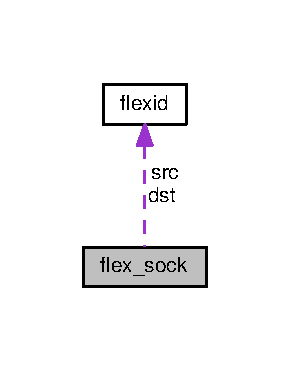
\includegraphics[width=139pt]{structflex__sock__coll__graph}
\end{center}
\end{figure}
\subsection*{Public Attributes}
\begin{DoxyCompactItemize}
\item 
struct sock \hyperlink{structflex__sock_a1ffc5042c0d6dd6b651ecb6a8e9b1096}{sk}
\item 
unsigned char \hyperlink{structflex__sock_acea083a0cc7f13d3491228dd261bfc70}{protocol}
\item 
short \hyperlink{structflex__sock_af4d0be6245faa22590e3d672d095a2a7}{message}
\item 
struct \hyperlink{structflexid}{flexid} \hyperlink{structflex__sock_a132b613c5f785e07196306bff98ef85d}{src}
\item 
struct \hyperlink{structflexid}{flexid} \hyperlink{structflex__sock_a1704e9612c290ef88bf674ea245b1835}{dst}
\item 
short \hyperlink{structflex__sock_afb460ef1d9e2fc1cc389ca5922f967d8}{addr\+\_\+type}
\item 
unsigned char \hyperlink{structflex__sock_a1c183d812ac68e320df127d58d303677}{addr\+\_\+len}
\item 
unsigned char \hyperlink{structflex__sock_a7c9d43f00ac325627f1396ffc10fe74a}{next\+\_\+hop} \mbox{[}M\+A\+X\+\_\+\+A\+D\+D\+R\+\_\+\+L\+EN\mbox{]}
\end{DoxyCompactItemize}


\subsection{Detailed Description}
The data structure for the Flex specified socket. 

\subsection{Member Data Documentation}
\index{flex\+\_\+sock@{flex\+\_\+sock}!addr\+\_\+len@{addr\+\_\+len}}
\index{addr\+\_\+len@{addr\+\_\+len}!flex\+\_\+sock@{flex\+\_\+sock}}
\subsubsection[{\texorpdfstring{addr\+\_\+len}{addr_len}}]{\setlength{\rightskip}{0pt plus 5cm}unsigned char flex\+\_\+sock\+::addr\+\_\+len}\hypertarget{structflex__sock_a1c183d812ac68e320df127d58d303677}{}\label{structflex__sock_a1c183d812ac68e320df127d58d303677}
The length of the address in the next hop \index{flex\+\_\+sock@{flex\+\_\+sock}!addr\+\_\+type@{addr\+\_\+type}}
\index{addr\+\_\+type@{addr\+\_\+type}!flex\+\_\+sock@{flex\+\_\+sock}}
\subsubsection[{\texorpdfstring{addr\+\_\+type}{addr_type}}]{\setlength{\rightskip}{0pt plus 5cm}short flex\+\_\+sock\+::addr\+\_\+type}\hypertarget{structflex__sock_afb460ef1d9e2fc1cc389ca5922f967d8}{}\label{structflex__sock_afb460ef1d9e2fc1cc389ca5922f967d8}
The address type of the next hop \index{flex\+\_\+sock@{flex\+\_\+sock}!dst@{dst}}
\index{dst@{dst}!flex\+\_\+sock@{flex\+\_\+sock}}
\subsubsection[{\texorpdfstring{dst}{dst}}]{\setlength{\rightskip}{0pt plus 5cm}struct {\bf flexid} flex\+\_\+sock\+::dst}\hypertarget{structflex__sock_a1704e9612c290ef88bf674ea245b1835}{}\label{structflex__sock_a1704e9612c290ef88bf674ea245b1835}
Flex ID of the destination \index{flex\+\_\+sock@{flex\+\_\+sock}!message@{message}}
\index{message@{message}!flex\+\_\+sock@{flex\+\_\+sock}}
\subsubsection[{\texorpdfstring{message}{message}}]{\setlength{\rightskip}{0pt plus 5cm}short flex\+\_\+sock\+::message}\hypertarget{structflex__sock_af4d0be6245faa22590e3d672d095a2a7}{}\label{structflex__sock_af4d0be6245faa22590e3d672d095a2a7}
The message type \index{flex\+\_\+sock@{flex\+\_\+sock}!next\+\_\+hop@{next\+\_\+hop}}
\index{next\+\_\+hop@{next\+\_\+hop}!flex\+\_\+sock@{flex\+\_\+sock}}
\subsubsection[{\texorpdfstring{next\+\_\+hop}{next_hop}}]{\setlength{\rightskip}{0pt plus 5cm}unsigned char flex\+\_\+sock\+::next\+\_\+hop\mbox{[}M\+A\+X\+\_\+\+A\+D\+D\+R\+\_\+\+L\+EN\mbox{]}}\hypertarget{structflex__sock_a7c9d43f00ac325627f1396ffc10fe74a}{}\label{structflex__sock_a7c9d43f00ac325627f1396ffc10fe74a}
The address of the next hop \index{flex\+\_\+sock@{flex\+\_\+sock}!protocol@{protocol}}
\index{protocol@{protocol}!flex\+\_\+sock@{flex\+\_\+sock}}
\subsubsection[{\texorpdfstring{protocol}{protocol}}]{\setlength{\rightskip}{0pt plus 5cm}unsigned char flex\+\_\+sock\+::protocol}\hypertarget{structflex__sock_acea083a0cc7f13d3491228dd261bfc70}{}\label{structflex__sock_acea083a0cc7f13d3491228dd261bfc70}
This member shows the reliable/unreliable communication is used \index{flex\+\_\+sock@{flex\+\_\+sock}!sk@{sk}}
\index{sk@{sk}!flex\+\_\+sock@{flex\+\_\+sock}}
\subsubsection[{\texorpdfstring{sk}{sk}}]{\setlength{\rightskip}{0pt plus 5cm}struct sock flex\+\_\+sock\+::sk}\hypertarget{structflex__sock_a1ffc5042c0d6dd6b651ecb6a8e9b1096}{}\label{structflex__sock_a1ffc5042c0d6dd6b651ecb6a8e9b1096}
This member contains the sock structure \index{flex\+\_\+sock@{flex\+\_\+sock}!src@{src}}
\index{src@{src}!flex\+\_\+sock@{flex\+\_\+sock}}
\subsubsection[{\texorpdfstring{src}{src}}]{\setlength{\rightskip}{0pt plus 5cm}struct {\bf flexid} flex\+\_\+sock\+::src}\hypertarget{structflex__sock_a132b613c5f785e07196306bff98ef85d}{}\label{structflex__sock_a132b613c5f785e07196306bff98ef85d}
Flex ID of the source 

The documentation for this struct was generated from the following file\+:\begin{DoxyCompactItemize}
\item 
socket/\hyperlink{flex__sock_8h}{flex\+\_\+sock.\+h}\end{DoxyCompactItemize}

\hypertarget{structflexhdr}{}\section{flexhdr Struct Reference}
\label{structflexhdr}\index{flexhdr@{flexhdr}}
\subsection*{Public Attributes}
\begin{DoxyCompactItemize}
\item 
\+\_\+\+\_\+u8 {\bfseries version}\hypertarget{structflexhdr_a58658c0c3ac88c2ae21cf52cdbeaefd0}{}\label{structflexhdr_a58658c0c3ac88c2ae21cf52cdbeaefd0}

\item 
\+\_\+\+\_\+u8 {\bfseries packet\+\_\+type}\hypertarget{structflexhdr_a3e17e4077f496e9eed85b5705a40b06f}{}\label{structflexhdr_a3e17e4077f496e9eed85b5705a40b06f}

\item 
\+\_\+\+\_\+u8 {\bfseries hash\+\_\+type}\hypertarget{structflexhdr_aa2a7292e9ff348680f83067955b58d0f}{}\label{structflexhdr_aa2a7292e9ff348680f83067955b58d0f}

\item 
\+\_\+\+\_\+u8 {\bfseries hop\+\_\+limit}\hypertarget{structflexhdr_a550e9254701dcd7665cdc1d52f9599fa}{}\label{structflexhdr_a550e9254701dcd7665cdc1d52f9599fa}

\item 
\+\_\+\+\_\+be16 {\bfseries header\+\_\+len}\hypertarget{structflexhdr_a7a2903458e61241565c61177a87c6dbb}{}\label{structflexhdr_a7a2903458e61241565c61177a87c6dbb}

\item 
\+\_\+\+\_\+sum16 {\bfseries check}\hypertarget{structflexhdr_a7e2d0c232c92ea39204ec52563cbd33e}{}\label{structflexhdr_a7e2d0c232c92ea39204ec52563cbd33e}

\item 
\+\_\+\+\_\+be16 {\bfseries packet\+\_\+id}\hypertarget{structflexhdr_a15281b3aa64868e176dffbb7ee5f2acc}{}\label{structflexhdr_a15281b3aa64868e176dffbb7ee5f2acc}

\item 
\+\_\+\+\_\+be16 {\bfseries frag\+\_\+off}\hypertarget{structflexhdr_a85f045e7acaf63edb2cd192266ef49bf}{}\label{structflexhdr_a85f045e7acaf63edb2cd192266ef49bf}

\item 
char {\bfseries sflex\+\_\+id} \mbox{[}F\+L\+E\+X\+\_\+\+I\+D\+\_\+\+L\+E\+N\+G\+TH\mbox{]}\hypertarget{structflexhdr_a3d0b687dac926a77cde8a5cc01f05533}{}\label{structflexhdr_a3d0b687dac926a77cde8a5cc01f05533}

\item 
char {\bfseries dflex\+\_\+id} \mbox{[}F\+L\+E\+X\+\_\+\+I\+D\+\_\+\+L\+E\+N\+G\+TH\mbox{]}\hypertarget{structflexhdr_aab2628ec55f6dedda9cd48de1677d49c}{}\label{structflexhdr_aab2628ec55f6dedda9cd48de1677d49c}

\item 
\+\_\+\+\_\+be16 {\bfseries packet\+\_\+len}\hypertarget{structflexhdr_a8e177eb08fa03f382eb67f75d9bf16b9}{}\label{structflexhdr_a8e177eb08fa03f382eb67f75d9bf16b9}

\item 
\+\_\+\+\_\+be32 {\bfseries seq}\hypertarget{structflexhdr_a1f437e344ae8752c7ea0586104bf67b4}{}\label{structflexhdr_a1f437e344ae8752c7ea0586104bf67b4}

\item 
\+\_\+\+\_\+be32 {\bfseries ack}\hypertarget{structflexhdr_a9504db4a12b79baa7937e1d11f521e57}{}\label{structflexhdr_a9504db4a12b79baa7937e1d11f521e57}

\end{DoxyCompactItemize}


The documentation for this struct was generated from the following files\+:\begin{DoxyCompactItemize}
\item 
apps/ipv4/proto\+\_\+flex.\+h\item 
include/flex/flex\+\_\+hdr.\+h\end{DoxyCompactItemize}

\hypertarget{structflexid}{}\section{flexid Struct Reference}
\label{structflexid}\index{flexid@{flexid}}


{\ttfamily \#include $<$flex\+\_\+id.\+h$>$}

\subsection*{Public Attributes}
\begin{DoxyCompactItemize}
\item 
\+\_\+\+\_\+u8 \hyperlink{structflexid_ab9e1df37109f8620f2be93955de9cb97}{identity} \mbox{[}20\mbox{]}
\item 
\+\_\+\+\_\+be32 \hyperlink{structflexid_a06122ad6fde6feb1e4edba60f476640e}{total\+\_\+segments}
\item 
\+\_\+\+\_\+be32 \hyperlink{structflexid_ae502fa12b4cd189628452ca8c6fd0dc0}{segment\+\_\+num}
\item 
\+\_\+\+\_\+be16 \hyperlink{structflexid_a652f4ff1a68f65a499f877337d4d7460}{length}
\end{DoxyCompactItemize}


\subsection{Member Data Documentation}
\index{flexid@{flexid}!identity@{identity}}
\index{identity@{identity}!flexid@{flexid}}
\subsubsection[{\texorpdfstring{identity}{identity}}]{\setlength{\rightskip}{0pt plus 5cm}\+\_\+\+\_\+u8 flexid\+::identity\mbox{[}20\mbox{]}}\hypertarget{structflexid_ab9e1df37109f8620f2be93955de9cb97}{}\label{structflexid_ab9e1df37109f8620f2be93955de9cb97}
\index{flexid@{flexid}!length@{length}}
\index{length@{length}!flexid@{flexid}}
\subsubsection[{\texorpdfstring{length}{length}}]{\setlength{\rightskip}{0pt plus 5cm}\+\_\+\+\_\+be16 flexid\+::length}\hypertarget{structflexid_a652f4ff1a68f65a499f877337d4d7460}{}\label{structflexid_a652f4ff1a68f65a499f877337d4d7460}
\index{flexid@{flexid}!segment\+\_\+num@{segment\+\_\+num}}
\index{segment\+\_\+num@{segment\+\_\+num}!flexid@{flexid}}
\subsubsection[{\texorpdfstring{segment\+\_\+num}{segment_num}}]{\setlength{\rightskip}{0pt plus 5cm}\+\_\+\+\_\+be32 flexid\+::segment\+\_\+num}\hypertarget{structflexid_ae502fa12b4cd189628452ca8c6fd0dc0}{}\label{structflexid_ae502fa12b4cd189628452ca8c6fd0dc0}
\index{flexid@{flexid}!total\+\_\+segments@{total\+\_\+segments}}
\index{total\+\_\+segments@{total\+\_\+segments}!flexid@{flexid}}
\subsubsection[{\texorpdfstring{total\+\_\+segments}{total_segments}}]{\setlength{\rightskip}{0pt plus 5cm}\+\_\+\+\_\+be32 flexid\+::total\+\_\+segments}\hypertarget{structflexid_a06122ad6fde6feb1e4edba60f476640e}{}\label{structflexid_a06122ad6fde6feb1e4edba60f476640e}


The documentation for this struct was generated from the following file\+:\begin{DoxyCompactItemize}
\item 
include/flex/\hyperlink{include_2flex_2flex__id_8h}{flex\+\_\+id.\+h}\end{DoxyCompactItemize}

\hypertarget{structflexidhdr}{}\section{flexidhdr Struct Reference}
\label{structflexidhdr}\index{flexidhdr@{flexidhdr}}


{\ttfamily \#include $<$flex\+\_\+id.\+h$>$}

\subsection*{Public Attributes}
\begin{DoxyCompactItemize}
\item 
uint8\+\_\+t \hyperlink{structflexidhdr_a040648453cb452e600995d86a1432264}{version}
\item 
uint8\+\_\+t \hyperlink{structflexidhdr_a0d1be6716bc037d0742bb7905c554b7d}{packet\+\_\+type}
\item 
uint8\+\_\+t \hyperlink{structflexidhdr_a4664d30de167966734c63a9602aa67d8}{hash\+\_\+type}
\item 
uint8\+\_\+t \hyperlink{structflexidhdr_ac0e058519cc822eb3cb525217bda557f}{hash\+\_\+len}
\item 
uint16\+\_\+t \hyperlink{structflexidhdr_a25cbbee361b8bff5511611a5f72cff57}{packet\+\_\+len}
\item 
uint16\+\_\+t \hyperlink{structflexidhdr_ae1825703c47432515e7eddb823e3489f}{checksum}
\item 
uint16\+\_\+t \hyperlink{structflexidhdr_a1fc7a84deb9e0042941f7c983f240691}{packet\+\_\+id}
\item 
uint16\+\_\+t \hyperlink{structflexidhdr_a7aa77d8aec125c11801198ca617e5ebe}{frag\+\_\+off}
\item 
uint16\+\_\+t \hyperlink{structflexidhdr_a1e5f6919e501e8aef925b4d78095ea06}{header\+\_\+len}
\item 
uint8\+\_\+t \hyperlink{structflexidhdr_a507914601558d094837046884f9b4d79}{hop\+\_\+limit}
\item 
uint8\+\_\+t \hyperlink{structflexidhdr_a79659668b865b2f14a1e5ac5e6ee63d5}{reserved}
\item 
uint8\+\_\+t $\ast$ \hyperlink{structflexidhdr_ae5f70fa4b298c9ff8fd8ac56d94f52ab}{saddr}
\item 
uint8\+\_\+t $\ast$ \hyperlink{structflexidhdr_a9eb9cfa99f8f77520244cd96d55145f5}{daddr}
\end{DoxyCompactItemize}


\subsection{Member Data Documentation}
\index{flexidhdr@{flexidhdr}!checksum@{checksum}}
\index{checksum@{checksum}!flexidhdr@{flexidhdr}}
\subsubsection[{\texorpdfstring{checksum}{checksum}}]{\setlength{\rightskip}{0pt plus 5cm}uint16\+\_\+t flexidhdr\+::checksum}\hypertarget{structflexidhdr_ae1825703c47432515e7eddb823e3489f}{}\label{structflexidhdr_ae1825703c47432515e7eddb823e3489f}
\index{flexidhdr@{flexidhdr}!daddr@{daddr}}
\index{daddr@{daddr}!flexidhdr@{flexidhdr}}
\subsubsection[{\texorpdfstring{daddr}{daddr}}]{\setlength{\rightskip}{0pt plus 5cm}uint8\+\_\+t$\ast$ flexidhdr\+::daddr}\hypertarget{structflexidhdr_a9eb9cfa99f8f77520244cd96d55145f5}{}\label{structflexidhdr_a9eb9cfa99f8f77520244cd96d55145f5}
\index{flexidhdr@{flexidhdr}!frag\+\_\+off@{frag\+\_\+off}}
\index{frag\+\_\+off@{frag\+\_\+off}!flexidhdr@{flexidhdr}}
\subsubsection[{\texorpdfstring{frag\+\_\+off}{frag_off}}]{\setlength{\rightskip}{0pt plus 5cm}uint16\+\_\+t flexidhdr\+::frag\+\_\+off}\hypertarget{structflexidhdr_a7aa77d8aec125c11801198ca617e5ebe}{}\label{structflexidhdr_a7aa77d8aec125c11801198ca617e5ebe}
\index{flexidhdr@{flexidhdr}!hash\+\_\+len@{hash\+\_\+len}}
\index{hash\+\_\+len@{hash\+\_\+len}!flexidhdr@{flexidhdr}}
\subsubsection[{\texorpdfstring{hash\+\_\+len}{hash_len}}]{\setlength{\rightskip}{0pt plus 5cm}uint8\+\_\+t flexidhdr\+::hash\+\_\+len}\hypertarget{structflexidhdr_ac0e058519cc822eb3cb525217bda557f}{}\label{structflexidhdr_ac0e058519cc822eb3cb525217bda557f}
\index{flexidhdr@{flexidhdr}!hash\+\_\+type@{hash\+\_\+type}}
\index{hash\+\_\+type@{hash\+\_\+type}!flexidhdr@{flexidhdr}}
\subsubsection[{\texorpdfstring{hash\+\_\+type}{hash_type}}]{\setlength{\rightskip}{0pt plus 5cm}uint8\+\_\+t flexidhdr\+::hash\+\_\+type}\hypertarget{structflexidhdr_a4664d30de167966734c63a9602aa67d8}{}\label{structflexidhdr_a4664d30de167966734c63a9602aa67d8}
\index{flexidhdr@{flexidhdr}!header\+\_\+len@{header\+\_\+len}}
\index{header\+\_\+len@{header\+\_\+len}!flexidhdr@{flexidhdr}}
\subsubsection[{\texorpdfstring{header\+\_\+len}{header_len}}]{\setlength{\rightskip}{0pt plus 5cm}uint16\+\_\+t flexidhdr\+::header\+\_\+len}\hypertarget{structflexidhdr_a1e5f6919e501e8aef925b4d78095ea06}{}\label{structflexidhdr_a1e5f6919e501e8aef925b4d78095ea06}
\index{flexidhdr@{flexidhdr}!hop\+\_\+limit@{hop\+\_\+limit}}
\index{hop\+\_\+limit@{hop\+\_\+limit}!flexidhdr@{flexidhdr}}
\subsubsection[{\texorpdfstring{hop\+\_\+limit}{hop_limit}}]{\setlength{\rightskip}{0pt plus 5cm}uint8\+\_\+t flexidhdr\+::hop\+\_\+limit}\hypertarget{structflexidhdr_a507914601558d094837046884f9b4d79}{}\label{structflexidhdr_a507914601558d094837046884f9b4d79}
\index{flexidhdr@{flexidhdr}!packet\+\_\+id@{packet\+\_\+id}}
\index{packet\+\_\+id@{packet\+\_\+id}!flexidhdr@{flexidhdr}}
\subsubsection[{\texorpdfstring{packet\+\_\+id}{packet_id}}]{\setlength{\rightskip}{0pt plus 5cm}uint16\+\_\+t flexidhdr\+::packet\+\_\+id}\hypertarget{structflexidhdr_a1fc7a84deb9e0042941f7c983f240691}{}\label{structflexidhdr_a1fc7a84deb9e0042941f7c983f240691}
\index{flexidhdr@{flexidhdr}!packet\+\_\+len@{packet\+\_\+len}}
\index{packet\+\_\+len@{packet\+\_\+len}!flexidhdr@{flexidhdr}}
\subsubsection[{\texorpdfstring{packet\+\_\+len}{packet_len}}]{\setlength{\rightskip}{0pt plus 5cm}uint16\+\_\+t flexidhdr\+::packet\+\_\+len}\hypertarget{structflexidhdr_a25cbbee361b8bff5511611a5f72cff57}{}\label{structflexidhdr_a25cbbee361b8bff5511611a5f72cff57}
\index{flexidhdr@{flexidhdr}!packet\+\_\+type@{packet\+\_\+type}}
\index{packet\+\_\+type@{packet\+\_\+type}!flexidhdr@{flexidhdr}}
\subsubsection[{\texorpdfstring{packet\+\_\+type}{packet_type}}]{\setlength{\rightskip}{0pt plus 5cm}uint8\+\_\+t flexidhdr\+::packet\+\_\+type}\hypertarget{structflexidhdr_a0d1be6716bc037d0742bb7905c554b7d}{}\label{structflexidhdr_a0d1be6716bc037d0742bb7905c554b7d}
\index{flexidhdr@{flexidhdr}!reserved@{reserved}}
\index{reserved@{reserved}!flexidhdr@{flexidhdr}}
\subsubsection[{\texorpdfstring{reserved}{reserved}}]{\setlength{\rightskip}{0pt plus 5cm}uint8\+\_\+t flexidhdr\+::reserved}\hypertarget{structflexidhdr_a79659668b865b2f14a1e5ac5e6ee63d5}{}\label{structflexidhdr_a79659668b865b2f14a1e5ac5e6ee63d5}
\index{flexidhdr@{flexidhdr}!saddr@{saddr}}
\index{saddr@{saddr}!flexidhdr@{flexidhdr}}
\subsubsection[{\texorpdfstring{saddr}{saddr}}]{\setlength{\rightskip}{0pt plus 5cm}uint8\+\_\+t$\ast$ flexidhdr\+::saddr}\hypertarget{structflexidhdr_ae5f70fa4b298c9ff8fd8ac56d94f52ab}{}\label{structflexidhdr_ae5f70fa4b298c9ff8fd8ac56d94f52ab}
\index{flexidhdr@{flexidhdr}!version@{version}}
\index{version@{version}!flexidhdr@{flexidhdr}}
\subsubsection[{\texorpdfstring{version}{version}}]{\setlength{\rightskip}{0pt plus 5cm}uint8\+\_\+t flexidhdr\+::version}\hypertarget{structflexidhdr_a040648453cb452e600995d86a1432264}{}\label{structflexidhdr_a040648453cb452e600995d86a1432264}


The documentation for this struct was generated from the following file\+:\begin{DoxyCompactItemize}
\item 
flexid/\hyperlink{flexid_2flex__id_8h}{flex\+\_\+id.\+h}\end{DoxyCompactItemize}

\hypertarget{structhash__entry}{}\section{hash\+\_\+entry Struct Reference}
\label{structhash__entry}\index{hash\+\_\+entry@{hash\+\_\+entry}}


{\ttfamily \#include $<$hash\+\_\+table.\+h$>$}



Collaboration diagram for hash\+\_\+entry\+:\nopagebreak
\begin{figure}[H]
\begin{center}
\leavevmode
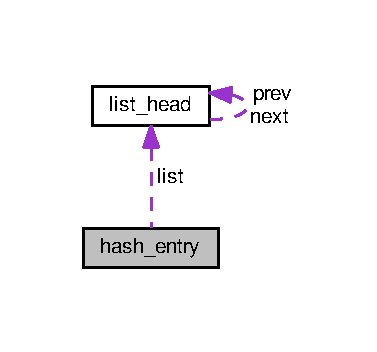
\includegraphics[width=181pt]{structhash__entry__coll__graph}
\end{center}
\end{figure}
\subsection*{Public Attributes}
\begin{DoxyCompactItemize}
\item 
struct \hyperlink{structlist__head}{list\+\_\+head} \hyperlink{structhash__entry_ada52d1b11e544cd19b58007cc3713069}{list}
\item 
unsigned char $\ast$ \hyperlink{structhash__entry_a0c23748b9dddd5f11b1ff9dbcbd47e9c}{key}
\item 
unsigned int \hyperlink{structhash__entry_a6f87c5657a590b7a848cc3f9a1d30d13}{keylen}
\end{DoxyCompactItemize}


\subsection{Member Data Documentation}
\index{hash\+\_\+entry@{hash\+\_\+entry}!key@{key}}
\index{key@{key}!hash\+\_\+entry@{hash\+\_\+entry}}
\subsubsection[{\texorpdfstring{key}{key}}]{\setlength{\rightskip}{0pt plus 5cm}unsigned char $\ast$ hash\+\_\+entry\+::key}\hypertarget{structhash__entry_a0c23748b9dddd5f11b1ff9dbcbd47e9c}{}\label{structhash__entry_a0c23748b9dddd5f11b1ff9dbcbd47e9c}
\index{hash\+\_\+entry@{hash\+\_\+entry}!keylen@{keylen}}
\index{keylen@{keylen}!hash\+\_\+entry@{hash\+\_\+entry}}
\subsubsection[{\texorpdfstring{keylen}{keylen}}]{\setlength{\rightskip}{0pt plus 5cm}unsigned int hash\+\_\+entry\+::keylen}\hypertarget{structhash__entry_a6f87c5657a590b7a848cc3f9a1d30d13}{}\label{structhash__entry_a6f87c5657a590b7a848cc3f9a1d30d13}
\index{hash\+\_\+entry@{hash\+\_\+entry}!list@{list}}
\index{list@{list}!hash\+\_\+entry@{hash\+\_\+entry}}
\subsubsection[{\texorpdfstring{list}{list}}]{\setlength{\rightskip}{0pt plus 5cm}struct {\bf list\+\_\+head} hash\+\_\+entry\+::list}\hypertarget{structhash__entry_ada52d1b11e544cd19b58007cc3713069}{}\label{structhash__entry_ada52d1b11e544cd19b58007cc3713069}


The documentation for this struct was generated from the following file\+:\begin{DoxyCompactItemize}
\item 
include/flex/\hyperlink{include_2flex_2hash__table_8h}{hash\+\_\+table.\+h}\end{DoxyCompactItemize}

\hypertarget{structhash__table}{}\section{hash\+\_\+table Struct Reference}
\label{structhash__table}\index{hash\+\_\+table@{hash\+\_\+table}}


{\ttfamily \#include $<$hash\+\_\+table.\+h$>$}



Collaboration diagram for hash\+\_\+table\+:\nopagebreak
\begin{figure}[H]
\begin{center}
\leavevmode
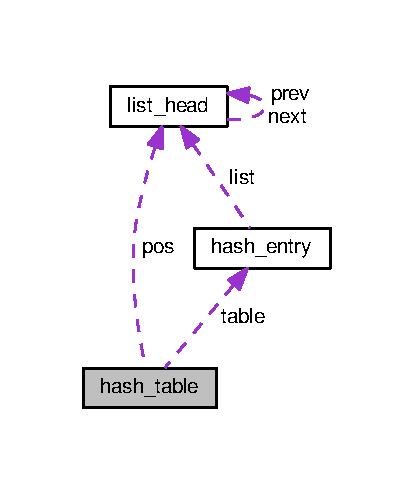
\includegraphics[width=199pt]{structhash__table__coll__graph}
\end{center}
\end{figure}
\subsection*{Public Attributes}
\begin{DoxyCompactItemize}
\item 
struct \hyperlink{structhash__entry}{hash\+\_\+entry} $\ast$ \hyperlink{structhash__table_a04cd18d2fc0ace3527670ceca050492b}{table}
\item 
unsigned int \hyperlink{structhash__table_a4678419b52c36e8b949b17eb4843a420}{buckets}
\item 
pthread\+\_\+mutex\+\_\+t $\ast$ \hyperlink{structhash__table_a4148c7a0d18b24d1c2961564dc0e7e7a}{bucket\+\_\+locks}
\item 
pthread\+\_\+mutex\+\_\+t \hyperlink{structhash__table_af4cefababf047c699eca5f45f8d4284e}{lock}
\item 
\hyperlink{util_2hash__table_8h_a9b0a83bb52986ea61f0e4351b66d41ef}{keycmp\+\_\+ptr} \hyperlink{structhash__table_a9465a319f391f0a50a4a84362c40fe48}{keycmp}
\item 
unsigned int \hyperlink{structhash__table_a77da69e21124ac1097627ae23ae72ef5}{\+\_\+\+\_\+ht\+\_\+i}
\item 
struct \hyperlink{structlist__head}{list\+\_\+head} $\ast$ \hyperlink{structhash__table_af9bcc20e562a8a4f6dd37aaa543a3883}{pos}
\end{DoxyCompactItemize}


\subsection{Member Data Documentation}
\index{hash\+\_\+table@{hash\+\_\+table}!\+\_\+\+\_\+ht\+\_\+i@{\+\_\+\+\_\+ht\+\_\+i}}
\index{\+\_\+\+\_\+ht\+\_\+i@{\+\_\+\+\_\+ht\+\_\+i}!hash\+\_\+table@{hash\+\_\+table}}
\subsubsection[{\texorpdfstring{\+\_\+\+\_\+ht\+\_\+i}{__ht_i}}]{\setlength{\rightskip}{0pt plus 5cm}unsigned int hash\+\_\+table\+::\+\_\+\+\_\+ht\+\_\+i}\hypertarget{structhash__table_a77da69e21124ac1097627ae23ae72ef5}{}\label{structhash__table_a77da69e21124ac1097627ae23ae72ef5}
\index{hash\+\_\+table@{hash\+\_\+table}!bucket\+\_\+locks@{bucket\+\_\+locks}}
\index{bucket\+\_\+locks@{bucket\+\_\+locks}!hash\+\_\+table@{hash\+\_\+table}}
\subsubsection[{\texorpdfstring{bucket\+\_\+locks}{bucket_locks}}]{\setlength{\rightskip}{0pt plus 5cm}pthread\+\_\+mutex\+\_\+t $\ast$ hash\+\_\+table\+::bucket\+\_\+locks}\hypertarget{structhash__table_a4148c7a0d18b24d1c2961564dc0e7e7a}{}\label{structhash__table_a4148c7a0d18b24d1c2961564dc0e7e7a}
\index{hash\+\_\+table@{hash\+\_\+table}!buckets@{buckets}}
\index{buckets@{buckets}!hash\+\_\+table@{hash\+\_\+table}}
\subsubsection[{\texorpdfstring{buckets}{buckets}}]{\setlength{\rightskip}{0pt plus 5cm}unsigned int hash\+\_\+table\+::buckets}\hypertarget{structhash__table_a4678419b52c36e8b949b17eb4843a420}{}\label{structhash__table_a4678419b52c36e8b949b17eb4843a420}
\index{hash\+\_\+table@{hash\+\_\+table}!keycmp@{keycmp}}
\index{keycmp@{keycmp}!hash\+\_\+table@{hash\+\_\+table}}
\subsubsection[{\texorpdfstring{keycmp}{keycmp}}]{\setlength{\rightskip}{0pt plus 5cm}{\bf keycmp\+\_\+ptr} hash\+\_\+table\+::keycmp}\hypertarget{structhash__table_a9465a319f391f0a50a4a84362c40fe48}{}\label{structhash__table_a9465a319f391f0a50a4a84362c40fe48}
\index{hash\+\_\+table@{hash\+\_\+table}!lock@{lock}}
\index{lock@{lock}!hash\+\_\+table@{hash\+\_\+table}}
\subsubsection[{\texorpdfstring{lock}{lock}}]{\setlength{\rightskip}{0pt plus 5cm}pthread\+\_\+mutex\+\_\+t hash\+\_\+table\+::lock}\hypertarget{structhash__table_af4cefababf047c699eca5f45f8d4284e}{}\label{structhash__table_af4cefababf047c699eca5f45f8d4284e}
\index{hash\+\_\+table@{hash\+\_\+table}!pos@{pos}}
\index{pos@{pos}!hash\+\_\+table@{hash\+\_\+table}}
\subsubsection[{\texorpdfstring{pos}{pos}}]{\setlength{\rightskip}{0pt plus 5cm}struct {\bf list\+\_\+head} $\ast$ hash\+\_\+table\+::pos}\hypertarget{structhash__table_af9bcc20e562a8a4f6dd37aaa543a3883}{}\label{structhash__table_af9bcc20e562a8a4f6dd37aaa543a3883}
\index{hash\+\_\+table@{hash\+\_\+table}!table@{table}}
\index{table@{table}!hash\+\_\+table@{hash\+\_\+table}}
\subsubsection[{\texorpdfstring{table}{table}}]{\setlength{\rightskip}{0pt plus 5cm}struct {\bf hash\+\_\+entry} $\ast$ hash\+\_\+table\+::table}\hypertarget{structhash__table_a04cd18d2fc0ace3527670ceca050492b}{}\label{structhash__table_a04cd18d2fc0ace3527670ceca050492b}


The documentation for this struct was generated from the following file\+:\begin{DoxyCompactItemize}
\item 
include/flex/\hyperlink{include_2flex_2hash__table_8h}{hash\+\_\+table.\+h}\end{DoxyCompactItemize}

\hypertarget{structid__manage__ops}{}\section{id\+\_\+manage\+\_\+ops Struct Reference}
\label{structid__manage__ops}\index{id\+\_\+manage\+\_\+ops@{id\+\_\+manage\+\_\+ops}}
\subsection*{Public Attributes}
\begin{DoxyCompactItemize}
\item 
int($\ast$ {\bfseries reg} )(\hyperlink{structflexid}{flexid\+\_\+t} $\ast$id)\hypertarget{structid__manage__ops_a1f5dd93a784407384a1cb31e34f212e2}{}\label{structid__manage__ops_a1f5dd93a784407384a1cb31e34f212e2}

\item 
int($\ast$ {\bfseries update} )(\hyperlink{structflexid}{flexid\+\_\+t} $\ast$id, unsigned char $\ast$key, unsigned char $\ast$value)\hypertarget{structid__manage__ops_a4a50cc4475967070b64333cfbc95b659}{}\label{structid__manage__ops_a4a50cc4475967070b64333cfbc95b659}

\item 
int($\ast$ {\bfseries request} )(\hyperlink{structflexid}{flexid\+\_\+t} $\ast$id)\hypertarget{structid__manage__ops_abd048ab844f857df4ffe671e6075770d}{}\label{structid__manage__ops_abd048ab844f857df4ffe671e6075770d}

\end{DoxyCompactItemize}


The documentation for this struct was generated from the following file\+:\begin{DoxyCompactItemize}
\item 
include/flex/id\+\_\+manage.\+h\end{DoxyCompactItemize}

\hypertarget{structlist__head}{}\section{list\+\_\+head Struct Reference}
\label{structlist__head}\index{list\+\_\+head@{list\+\_\+head}}


{\ttfamily \#include $<$list.\+h$>$}



Collaboration diagram for list\+\_\+head\+:\nopagebreak
\begin{figure}[H]
\begin{center}
\leavevmode
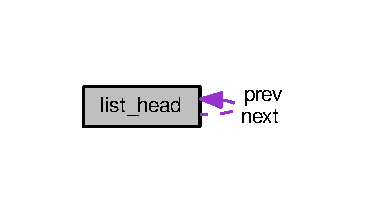
\includegraphics[width=176pt]{structlist__head__coll__graph}
\end{center}
\end{figure}
\subsection*{Public Attributes}
\begin{DoxyCompactItemize}
\item 
struct \hyperlink{structlist__head}{list\+\_\+head} $\ast$ \hyperlink{structlist__head_a44b2d28c78f7266869b3f00390bec772}{next}
\item 
struct \hyperlink{structlist__head}{list\+\_\+head} $\ast$ \hyperlink{structlist__head_aaa0eabda8877e1d6de73a33f223ad004}{prev}
\end{DoxyCompactItemize}


\subsection{Member Data Documentation}
\index{list\+\_\+head@{list\+\_\+head}!next@{next}}
\index{next@{next}!list\+\_\+head@{list\+\_\+head}}
\subsubsection[{\texorpdfstring{next}{next}}]{\setlength{\rightskip}{0pt plus 5cm}struct {\bf list\+\_\+head} $\ast$ list\+\_\+head\+::next}\hypertarget{structlist__head_a44b2d28c78f7266869b3f00390bec772}{}\label{structlist__head_a44b2d28c78f7266869b3f00390bec772}
\index{list\+\_\+head@{list\+\_\+head}!prev@{prev}}
\index{prev@{prev}!list\+\_\+head@{list\+\_\+head}}
\subsubsection[{\texorpdfstring{prev}{prev}}]{\setlength{\rightskip}{0pt plus 5cm}struct {\bf list\+\_\+head} $\ast$ list\+\_\+head\+::prev}\hypertarget{structlist__head_aaa0eabda8877e1d6de73a33f223ad004}{}\label{structlist__head_aaa0eabda8877e1d6de73a33f223ad004}


The documentation for this struct was generated from the following file\+:\begin{DoxyCompactItemize}
\item 
include/flex/\hyperlink{include_2flex_2list_8h}{list.\+h}\end{DoxyCompactItemize}

\hypertarget{structquery__list}{}\section{query\+\_\+list Struct Reference}
\label{structquery__list}\index{query\+\_\+list@{query\+\_\+list}}


The documentation for this struct was generated from the following file\+:\begin{DoxyCompactItemize}
\item 
include/flex/flex\+\_\+query.\+h\end{DoxyCompactItemize}

\hypertarget{structreply__list}{}\section{reply\+\_\+list Struct Reference}
\label{structreply__list}\index{reply\+\_\+list@{reply\+\_\+list}}


The documentation for this struct was generated from the following file\+:\begin{DoxyCompactItemize}
\item 
include/flex/flex\+\_\+query.\+h\end{DoxyCompactItemize}

\hypertarget{structrepo}{}\section{repo Struct Reference}
\label{structrepo}\index{repo@{repo}}


The documentation for this struct was generated from the following file\+:\begin{DoxyCompactItemize}
\item 
include/flex/flex\+\_\+repo.\+h\end{DoxyCompactItemize}

\hypertarget{structresponse}{}\section{response Struct Reference}
\label{structresponse}\index{response@{response}}


{\ttfamily \#include $<$flex\+\_\+request.\+h$>$}

\subsection*{Public Attributes}
\begin{DoxyCompactItemize}
\item 
short \hyperlink{structresponse_ae098504ec8fd2c1eafd3b8487a783575}{error}
\item 
short \hyperlink{structresponse_a2f45198ba85a80efc09cbde6098af0b8}{addr\+\_\+type}
\item 
unsigned char \hyperlink{structresponse_a835f830c6f09ed6b0e702b3021f66a57}{addr\+\_\+len}
\item 
unsigned char \hyperlink{structresponse_a6b7eac313932e975cd88a0d998867bb3}{next\+\_\+hop} \mbox{[}\hyperlink{flex__addr_8h_a13b71bf0266170fc990217b80b27f40d}{M\+A\+X\+\_\+\+A\+D\+D\+R\+E\+S\+S\+\_\+\+L\+E\+N\+G\+TH}\mbox{]}
\end{DoxyCompactItemize}


\subsection{Member Data Documentation}
\index{response@{response}!addr\+\_\+len@{addr\+\_\+len}}
\index{addr\+\_\+len@{addr\+\_\+len}!response@{response}}
\subsubsection[{\texorpdfstring{addr\+\_\+len}{addr_len}}]{\setlength{\rightskip}{0pt plus 5cm}unsigned char response\+::addr\+\_\+len}\hypertarget{structresponse_a835f830c6f09ed6b0e702b3021f66a57}{}\label{structresponse_a835f830c6f09ed6b0e702b3021f66a57}
\index{response@{response}!addr\+\_\+type@{addr\+\_\+type}}
\index{addr\+\_\+type@{addr\+\_\+type}!response@{response}}
\subsubsection[{\texorpdfstring{addr\+\_\+type}{addr_type}}]{\setlength{\rightskip}{0pt plus 5cm}short response\+::addr\+\_\+type}\hypertarget{structresponse_a2f45198ba85a80efc09cbde6098af0b8}{}\label{structresponse_a2f45198ba85a80efc09cbde6098af0b8}
\index{response@{response}!error@{error}}
\index{error@{error}!response@{response}}
\subsubsection[{\texorpdfstring{error}{error}}]{\setlength{\rightskip}{0pt plus 5cm}short response\+::error}\hypertarget{structresponse_ae098504ec8fd2c1eafd3b8487a783575}{}\label{structresponse_ae098504ec8fd2c1eafd3b8487a783575}
\index{response@{response}!next\+\_\+hop@{next\+\_\+hop}}
\index{next\+\_\+hop@{next\+\_\+hop}!response@{response}}
\subsubsection[{\texorpdfstring{next\+\_\+hop}{next_hop}}]{\setlength{\rightskip}{0pt plus 5cm}unsigned char response\+::next\+\_\+hop\mbox{[}{\bf M\+A\+X\+\_\+\+A\+D\+D\+R\+E\+S\+S\+\_\+\+L\+E\+N\+G\+TH}\mbox{]}}\hypertarget{structresponse_a6b7eac313932e975cd88a0d998867bb3}{}\label{structresponse_a6b7eac313932e975cd88a0d998867bb3}


The documentation for this struct was generated from the following file\+:\begin{DoxyCompactItemize}
\item 
include/flex/\hyperlink{flex__request_8h}{flex\+\_\+request.\+h}\end{DoxyCompactItemize}

\hypertarget{structrflexhdr}{}\section{rflexhdr Struct Reference}
\label{structrflexhdr}\index{rflexhdr@{rflexhdr}}


Collaboration diagram for rflexhdr\+:\nopagebreak
\begin{figure}[H]
\begin{center}
\leavevmode
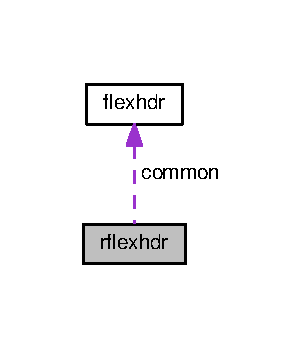
\includegraphics[width=146pt]{structrflexhdr__coll__graph}
\end{center}
\end{figure}
\subsection*{Public Attributes}
\begin{DoxyCompactItemize}
\item 
struct \hyperlink{structflexhdr}{flexhdr} {\bfseries common}\hypertarget{structrflexhdr_a0e80ead5eb57aba13d18f75f0906569c}{}\label{structrflexhdr_a0e80ead5eb57aba13d18f75f0906569c}

\item 
char {\bfseries sflex\+\_\+id} \mbox{[}F\+L\+E\+X\+\_\+\+I\+D\+\_\+\+L\+E\+N\+G\+TH\mbox{]}\hypertarget{structrflexhdr_aa79b53451e65228d567880e512cadc3e}{}\label{structrflexhdr_aa79b53451e65228d567880e512cadc3e}

\item 
char {\bfseries dflex\+\_\+id} \mbox{[}F\+L\+E\+X\+\_\+\+I\+D\+\_\+\+L\+E\+N\+G\+TH\mbox{]}\hypertarget{structrflexhdr_a091799a62ae442e024334d0eb4cb86b6}{}\label{structrflexhdr_a091799a62ae442e024334d0eb4cb86b6}

\item 
\+\_\+\+\_\+be16 {\bfseries packet\+\_\+len}\hypertarget{structrflexhdr_a2cc8c14fec43032de69ef360ffc4dfbe}{}\label{structrflexhdr_a2cc8c14fec43032de69ef360ffc4dfbe}

\item 
\+\_\+\+\_\+be32 {\bfseries seq}\hypertarget{structrflexhdr_a5ef194bf9db68ec8f6b050ca9608bd75}{}\label{structrflexhdr_a5ef194bf9db68ec8f6b050ca9608bd75}

\item 
\+\_\+\+\_\+be32 {\bfseries ack}\hypertarget{structrflexhdr_ae799b07034366e7e68c5b441f816e183}{}\label{structrflexhdr_ae799b07034366e7e68c5b441f816e183}

\end{DoxyCompactItemize}


The documentation for this struct was generated from the following file\+:\begin{DoxyCompactItemize}
\item 
include/flex/flex\+\_\+hdr.\+h\end{DoxyCompactItemize}

\hypertarget{structrflexhdr__ext}{}\section{rflexhdr\+\_\+ext Struct Reference}
\label{structrflexhdr__ext}\index{rflexhdr\+\_\+ext@{rflexhdr\+\_\+ext}}


Collaboration diagram for rflexhdr\+\_\+ext\+:\nopagebreak
\begin{figure}[H]
\begin{center}
\leavevmode
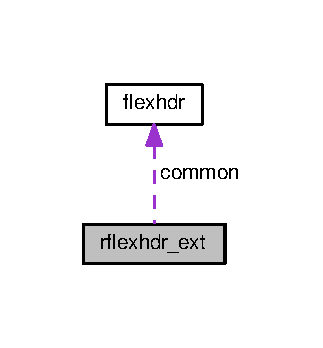
\includegraphics[width=155pt]{structrflexhdr__ext__coll__graph}
\end{center}
\end{figure}
\subsection*{Public Attributes}
\begin{DoxyCompactItemize}
\item 
struct \hyperlink{structflexhdr}{flexhdr} {\bfseries common}\hypertarget{structrflexhdr__ext_ac57a5553651d7cdde22b2d00c0a916ce}{}\label{structrflexhdr__ext_ac57a5553651d7cdde22b2d00c0a916ce}

\item 
char {\bfseries sflex\+\_\+id} \mbox{[}F\+L\+E\+X\+\_\+\+I\+D\+\_\+\+E\+X\+T\+\_\+\+L\+E\+N\+G\+TH\mbox{]}\hypertarget{structrflexhdr__ext_aba2b1333b35892ce3ae9c75dd8e2a521}{}\label{structrflexhdr__ext_aba2b1333b35892ce3ae9c75dd8e2a521}

\item 
char {\bfseries dflex\+\_\+id} \mbox{[}F\+L\+E\+X\+\_\+\+I\+D\+\_\+\+E\+X\+T\+\_\+\+L\+E\+N\+G\+TH\mbox{]}\hypertarget{structrflexhdr__ext_a3e35c1161803908776955800eb2ad3fe}{}\label{structrflexhdr__ext_a3e35c1161803908776955800eb2ad3fe}

\item 
\+\_\+\+\_\+be16 {\bfseries packet\+\_\+len}\hypertarget{structrflexhdr__ext_ac716297c579ced38da559cf53967f09b}{}\label{structrflexhdr__ext_ac716297c579ced38da559cf53967f09b}

\item 
\+\_\+\+\_\+be32 {\bfseries seq}\hypertarget{structrflexhdr__ext_a240fcbc0eff91a233304845f516d75d8}{}\label{structrflexhdr__ext_a240fcbc0eff91a233304845f516d75d8}

\item 
\+\_\+\+\_\+be32 {\bfseries ack}\hypertarget{structrflexhdr__ext_aee0018851d2f3381fd99c405606731b4}{}\label{structrflexhdr__ext_aee0018851d2f3381fd99c405606731b4}

\end{DoxyCompactItemize}


The documentation for this struct was generated from the following file\+:\begin{DoxyCompactItemize}
\item 
include/flex/flex\+\_\+hdr.\+h\end{DoxyCompactItemize}

\hypertarget{structsockaddr__flex}{}\section{sockaddr\+\_\+flex Struct Reference}
\label{structsockaddr__flex}\index{sockaddr\+\_\+flex@{sockaddr\+\_\+flex}}


{\ttfamily \#include $<$flex\+\_\+socket.\+h$>$}



Collaboration diagram for sockaddr\+\_\+flex\+:\nopagebreak
\begin{figure}[H]
\begin{center}
\leavevmode
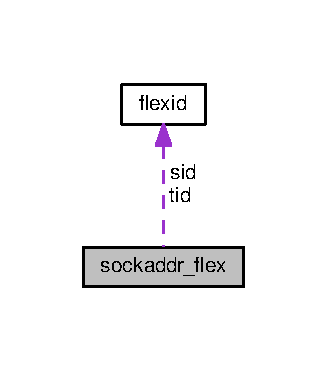
\includegraphics[width=157pt]{structsockaddr__flex__coll__graph}
\end{center}
\end{figure}
\subsection*{Public Attributes}
\begin{DoxyCompactItemize}
\item 
\+\_\+\+\_\+kernel\+\_\+sa\+\_\+family\+\_\+t \hyperlink{structsockaddr__flex_a0bebb0734429c3e6a548fc61de27c9c0}{sin\+\_\+family}
\item 
struct \hyperlink{structflexid}{flexid} \hyperlink{structsockaddr__flex_ae2d332f61042d379e3521f7e42603037}{sid}
\item 
struct \hyperlink{structflexid}{flexid} \hyperlink{structsockaddr__flex_a841742293b927751d2c0f8c48d7a5828}{tid}
\item 
short \hyperlink{structsockaddr__flex_ac1581ee2d027808218f3173c372924a1}{message}
\item 
short \hyperlink{structsockaddr__flex_a8945354761455603e8f09077e454defe}{addr\+\_\+type}
\item 
unsigned char \hyperlink{structsockaddr__flex_a44a4c4cabcecc77838283ed0a2fe22bb}{addr\+\_\+len}
\item 
unsigned char \hyperlink{structsockaddr__flex_a6869850bbb4ae164d955372332fffee3}{next\+\_\+hop} \mbox{[}\hyperlink{flex__addr_8h_a13b71bf0266170fc990217b80b27f40d}{M\+A\+X\+\_\+\+A\+D\+D\+R\+E\+S\+S\+\_\+\+L\+E\+N\+G\+TH}\mbox{]}
\end{DoxyCompactItemize}


\subsection{Member Data Documentation}
\index{sockaddr\+\_\+flex@{sockaddr\+\_\+flex}!addr\+\_\+len@{addr\+\_\+len}}
\index{addr\+\_\+len@{addr\+\_\+len}!sockaddr\+\_\+flex@{sockaddr\+\_\+flex}}
\subsubsection[{\texorpdfstring{addr\+\_\+len}{addr_len}}]{\setlength{\rightskip}{0pt plus 5cm}unsigned char sockaddr\+\_\+flex\+::addr\+\_\+len}\hypertarget{structsockaddr__flex_a44a4c4cabcecc77838283ed0a2fe22bb}{}\label{structsockaddr__flex_a44a4c4cabcecc77838283ed0a2fe22bb}
\index{sockaddr\+\_\+flex@{sockaddr\+\_\+flex}!addr\+\_\+type@{addr\+\_\+type}}
\index{addr\+\_\+type@{addr\+\_\+type}!sockaddr\+\_\+flex@{sockaddr\+\_\+flex}}
\subsubsection[{\texorpdfstring{addr\+\_\+type}{addr_type}}]{\setlength{\rightskip}{0pt plus 5cm}short sockaddr\+\_\+flex\+::addr\+\_\+type}\hypertarget{structsockaddr__flex_a8945354761455603e8f09077e454defe}{}\label{structsockaddr__flex_a8945354761455603e8f09077e454defe}
\index{sockaddr\+\_\+flex@{sockaddr\+\_\+flex}!message@{message}}
\index{message@{message}!sockaddr\+\_\+flex@{sockaddr\+\_\+flex}}
\subsubsection[{\texorpdfstring{message}{message}}]{\setlength{\rightskip}{0pt plus 5cm}short sockaddr\+\_\+flex\+::message}\hypertarget{structsockaddr__flex_ac1581ee2d027808218f3173c372924a1}{}\label{structsockaddr__flex_ac1581ee2d027808218f3173c372924a1}
\index{sockaddr\+\_\+flex@{sockaddr\+\_\+flex}!next\+\_\+hop@{next\+\_\+hop}}
\index{next\+\_\+hop@{next\+\_\+hop}!sockaddr\+\_\+flex@{sockaddr\+\_\+flex}}
\subsubsection[{\texorpdfstring{next\+\_\+hop}{next_hop}}]{\setlength{\rightskip}{0pt plus 5cm}unsigned char sockaddr\+\_\+flex\+::next\+\_\+hop\mbox{[}{\bf M\+A\+X\+\_\+\+A\+D\+D\+R\+E\+S\+S\+\_\+\+L\+E\+N\+G\+TH}\mbox{]}}\hypertarget{structsockaddr__flex_a6869850bbb4ae164d955372332fffee3}{}\label{structsockaddr__flex_a6869850bbb4ae164d955372332fffee3}
\index{sockaddr\+\_\+flex@{sockaddr\+\_\+flex}!sid@{sid}}
\index{sid@{sid}!sockaddr\+\_\+flex@{sockaddr\+\_\+flex}}
\subsubsection[{\texorpdfstring{sid}{sid}}]{\setlength{\rightskip}{0pt plus 5cm}struct {\bf flexid} sockaddr\+\_\+flex\+::sid}\hypertarget{structsockaddr__flex_ae2d332f61042d379e3521f7e42603037}{}\label{structsockaddr__flex_ae2d332f61042d379e3521f7e42603037}
\index{sockaddr\+\_\+flex@{sockaddr\+\_\+flex}!sin\+\_\+family@{sin\+\_\+family}}
\index{sin\+\_\+family@{sin\+\_\+family}!sockaddr\+\_\+flex@{sockaddr\+\_\+flex}}
\subsubsection[{\texorpdfstring{sin\+\_\+family}{sin_family}}]{\setlength{\rightskip}{0pt plus 5cm}\+\_\+\+\_\+kernel\+\_\+sa\+\_\+family\+\_\+t sockaddr\+\_\+flex\+::sin\+\_\+family}\hypertarget{structsockaddr__flex_a0bebb0734429c3e6a548fc61de27c9c0}{}\label{structsockaddr__flex_a0bebb0734429c3e6a548fc61de27c9c0}
\index{sockaddr\+\_\+flex@{sockaddr\+\_\+flex}!tid@{tid}}
\index{tid@{tid}!sockaddr\+\_\+flex@{sockaddr\+\_\+flex}}
\subsubsection[{\texorpdfstring{tid}{tid}}]{\setlength{\rightskip}{0pt plus 5cm}struct {\bf flexid} sockaddr\+\_\+flex\+::tid}\hypertarget{structsockaddr__flex_a841742293b927751d2c0f8c48d7a5828}{}\label{structsockaddr__flex_a841742293b927751d2c0f8c48d7a5828}


The documentation for this struct was generated from the following file\+:\begin{DoxyCompactItemize}
\item 
include/flex/\hyperlink{flex__socket_8h}{flex\+\_\+socket.\+h}\end{DoxyCompactItemize}

\hypertarget{structu__hslot}{}\section{u\+\_\+hslot Struct Reference}
\label{structu__hslot}\index{u\+\_\+hslot@{u\+\_\+hslot}}
\subsection*{Public Attributes}
\begin{DoxyCompactItemize}
\item 
struct hlist\+\_\+nulls\+\_\+head {\bfseries head}\hypertarget{structu__hslot_abe6060ce741ff9e94d6f4669ec7f4c9a}{}\label{structu__hslot_abe6060ce741ff9e94d6f4669ec7f4c9a}

\item 
int {\bfseries count}\hypertarget{structu__hslot_a2eee707762aa72c4d82f24d0422efa19}{}\label{structu__hslot_a2eee707762aa72c4d82f24d0422efa19}

\item 
spinlock\+\_\+t {\bfseries lock}\hypertarget{structu__hslot_a3a866b196889821639c6d1aa91af6154}{}\label{structu__hslot_a3a866b196889821639c6d1aa91af6154}

\end{DoxyCompactItemize}


The documentation for this struct was generated from the following file\+:\begin{DoxyCompactItemize}
\item 
socket/flex\+\_\+unreliable.\+h\end{DoxyCompactItemize}

\hypertarget{structu__table}{}\section{u\+\_\+table Struct Reference}
\label{structu__table}\index{u\+\_\+table@{u\+\_\+table}}


{\ttfamily \#include $<$flex\+\_\+unreliable.\+h$>$}



Collaboration diagram for u\+\_\+table\+:\nopagebreak
\begin{figure}[H]
\begin{center}
\leavevmode
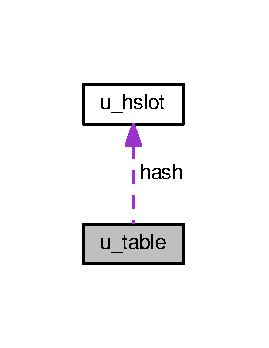
\includegraphics[width=129pt]{structu__table__coll__graph}
\end{center}
\end{figure}
\subsection*{Public Attributes}
\begin{DoxyCompactItemize}
\item 
struct \hyperlink{structu__hslot}{u\+\_\+hslot} $\ast$ \hyperlink{structu__table_a9d4512b1f9f38f0a6a24841ce2ca32a6}{hash}
\item 
unsigned int \hyperlink{structu__table_aeb1108e804777cac0e332f0310a78f09}{mask}
\item 
unsigned int \hyperlink{structu__table_ab9c33f2ba15bf3544b0176fbe59ccecd}{log}
\end{DoxyCompactItemize}


\subsection{Member Data Documentation}
\index{u\+\_\+table@{u\+\_\+table}!hash@{hash}}
\index{hash@{hash}!u\+\_\+table@{u\+\_\+table}}
\subsubsection[{\texorpdfstring{hash}{hash}}]{\setlength{\rightskip}{0pt plus 5cm}struct {\bf u\+\_\+hslot}$\ast$ u\+\_\+table\+::hash}\hypertarget{structu__table_a9d4512b1f9f38f0a6a24841ce2ca32a6}{}\label{structu__table_a9d4512b1f9f38f0a6a24841ce2ca32a6}
\index{u\+\_\+table@{u\+\_\+table}!log@{log}}
\index{log@{log}!u\+\_\+table@{u\+\_\+table}}
\subsubsection[{\texorpdfstring{log}{log}}]{\setlength{\rightskip}{0pt plus 5cm}unsigned int u\+\_\+table\+::log}\hypertarget{structu__table_ab9c33f2ba15bf3544b0176fbe59ccecd}{}\label{structu__table_ab9c33f2ba15bf3544b0176fbe59ccecd}
\index{u\+\_\+table@{u\+\_\+table}!mask@{mask}}
\index{mask@{mask}!u\+\_\+table@{u\+\_\+table}}
\subsubsection[{\texorpdfstring{mask}{mask}}]{\setlength{\rightskip}{0pt plus 5cm}unsigned int u\+\_\+table\+::mask}\hypertarget{structu__table_aeb1108e804777cac0e332f0310a78f09}{}\label{structu__table_aeb1108e804777cac0e332f0310a78f09}


The documentation for this struct was generated from the following file\+:\begin{DoxyCompactItemize}
\item 
socket/\hyperlink{flex__unreliable_8h}{flex\+\_\+unreliable.\+h}\end{DoxyCompactItemize}

\hypertarget{structuflexhdr}{}\section{uflexhdr Struct Reference}
\label{structuflexhdr}\index{uflexhdr@{uflexhdr}}


{\ttfamily \#include $<$flex\+\_\+hdr.\+h$>$}



Collaboration diagram for uflexhdr\+:\nopagebreak
\begin{figure}[H]
\begin{center}
\leavevmode
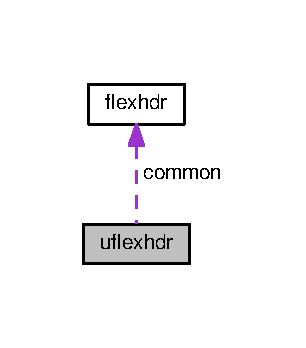
\includegraphics[width=147pt]{structuflexhdr__coll__graph}
\end{center}
\end{figure}
\subsection*{Public Attributes}
\begin{DoxyCompactItemize}
\item 
struct \hyperlink{structflexhdr}{flexhdr} \hyperlink{structuflexhdr_a298ecaecd1223467c1820a652458cff9}{common}
\item 
char \hyperlink{structuflexhdr_a359db5a95d160b5bacdde8883a9d1ee7}{sflex\+\_\+id} \mbox{[}\hyperlink{flex__const_8h_a342f27a8d723d83c803e6d934f999ada}{F\+L\+E\+X\+\_\+\+I\+D\+\_\+\+L\+E\+N\+G\+TH}\mbox{]}
\item 
char \hyperlink{structuflexhdr_a8733c5298ef2cdefd132ecec4878605f}{dflex\+\_\+id} \mbox{[}\hyperlink{flex__const_8h_a342f27a8d723d83c803e6d934f999ada}{F\+L\+E\+X\+\_\+\+I\+D\+\_\+\+L\+E\+N\+G\+TH}\mbox{]}
\item 
\+\_\+\+\_\+be16 \hyperlink{structuflexhdr_a633f53e21cbca9248040e940553af36e}{packet\+\_\+len}
\end{DoxyCompactItemize}


\subsection{Member Data Documentation}
\index{uflexhdr@{uflexhdr}!common@{common}}
\index{common@{common}!uflexhdr@{uflexhdr}}
\subsubsection[{\texorpdfstring{common}{common}}]{\setlength{\rightskip}{0pt plus 5cm}struct {\bf flexhdr} uflexhdr\+::common}\hypertarget{structuflexhdr_a298ecaecd1223467c1820a652458cff9}{}\label{structuflexhdr_a298ecaecd1223467c1820a652458cff9}
\index{uflexhdr@{uflexhdr}!dflex\+\_\+id@{dflex\+\_\+id}}
\index{dflex\+\_\+id@{dflex\+\_\+id}!uflexhdr@{uflexhdr}}
\subsubsection[{\texorpdfstring{dflex\+\_\+id}{dflex_id}}]{\setlength{\rightskip}{0pt plus 5cm}char uflexhdr\+::dflex\+\_\+id\mbox{[}{\bf F\+L\+E\+X\+\_\+\+I\+D\+\_\+\+L\+E\+N\+G\+TH}\mbox{]}}\hypertarget{structuflexhdr_a8733c5298ef2cdefd132ecec4878605f}{}\label{structuflexhdr_a8733c5298ef2cdefd132ecec4878605f}
\index{uflexhdr@{uflexhdr}!packet\+\_\+len@{packet\+\_\+len}}
\index{packet\+\_\+len@{packet\+\_\+len}!uflexhdr@{uflexhdr}}
\subsubsection[{\texorpdfstring{packet\+\_\+len}{packet_len}}]{\setlength{\rightskip}{0pt plus 5cm}\+\_\+\+\_\+be16 uflexhdr\+::packet\+\_\+len}\hypertarget{structuflexhdr_a633f53e21cbca9248040e940553af36e}{}\label{structuflexhdr_a633f53e21cbca9248040e940553af36e}
\index{uflexhdr@{uflexhdr}!sflex\+\_\+id@{sflex\+\_\+id}}
\index{sflex\+\_\+id@{sflex\+\_\+id}!uflexhdr@{uflexhdr}}
\subsubsection[{\texorpdfstring{sflex\+\_\+id}{sflex_id}}]{\setlength{\rightskip}{0pt plus 5cm}char uflexhdr\+::sflex\+\_\+id\mbox{[}{\bf F\+L\+E\+X\+\_\+\+I\+D\+\_\+\+L\+E\+N\+G\+TH}\mbox{]}}\hypertarget{structuflexhdr_a359db5a95d160b5bacdde8883a9d1ee7}{}\label{structuflexhdr_a359db5a95d160b5bacdde8883a9d1ee7}


The documentation for this struct was generated from the following file\+:\begin{DoxyCompactItemize}
\item 
include/flex/\hyperlink{flex__hdr_8h}{flex\+\_\+hdr.\+h}\end{DoxyCompactItemize}

\hypertarget{structuflexhdr__ext}{}\section{uflexhdr\+\_\+ext Struct Reference}
\label{structuflexhdr__ext}\index{uflexhdr\+\_\+ext@{uflexhdr\+\_\+ext}}


{\ttfamily \#include $<$flex\+\_\+hdr.\+h$>$}



Collaboration diagram for uflexhdr\+\_\+ext\+:\nopagebreak
\begin{figure}[H]
\begin{center}
\leavevmode
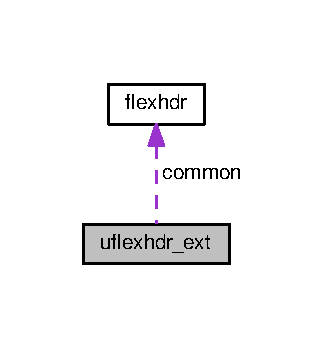
\includegraphics[width=156pt]{structuflexhdr__ext__coll__graph}
\end{center}
\end{figure}
\subsection*{Public Attributes}
\begin{DoxyCompactItemize}
\item 
struct \hyperlink{structflexhdr}{flexhdr} \hyperlink{structuflexhdr__ext_af481d03a7524a0f483e6fd8877c00563}{common}
\item 
char \hyperlink{structuflexhdr__ext_abf9a4c10efddc6b46acf9e25915cdcb3}{sflex\+\_\+id} \mbox{[}\hyperlink{flex__const_8h_a5bfdaffe9863d3fcfc3b90fa2a893bfd}{F\+L\+E\+X\+\_\+\+I\+D\+\_\+\+E\+X\+T\+\_\+\+L\+E\+N\+G\+TH}\mbox{]}
\item 
char \hyperlink{structuflexhdr__ext_a61d75d5fd362fb576a53fa8f973c2380}{dflex\+\_\+id} \mbox{[}\hyperlink{flex__const_8h_a5bfdaffe9863d3fcfc3b90fa2a893bfd}{F\+L\+E\+X\+\_\+\+I\+D\+\_\+\+E\+X\+T\+\_\+\+L\+E\+N\+G\+TH}\mbox{]}
\item 
\+\_\+\+\_\+be16 \hyperlink{structuflexhdr__ext_aa8dd1115a6af281d1a91102926d5cd4d}{packet\+\_\+len}
\end{DoxyCompactItemize}


\subsection{Member Data Documentation}
\index{uflexhdr\+\_\+ext@{uflexhdr\+\_\+ext}!common@{common}}
\index{common@{common}!uflexhdr\+\_\+ext@{uflexhdr\+\_\+ext}}
\subsubsection[{\texorpdfstring{common}{common}}]{\setlength{\rightskip}{0pt plus 5cm}struct {\bf flexhdr} uflexhdr\+\_\+ext\+::common}\hypertarget{structuflexhdr__ext_af481d03a7524a0f483e6fd8877c00563}{}\label{structuflexhdr__ext_af481d03a7524a0f483e6fd8877c00563}
\index{uflexhdr\+\_\+ext@{uflexhdr\+\_\+ext}!dflex\+\_\+id@{dflex\+\_\+id}}
\index{dflex\+\_\+id@{dflex\+\_\+id}!uflexhdr\+\_\+ext@{uflexhdr\+\_\+ext}}
\subsubsection[{\texorpdfstring{dflex\+\_\+id}{dflex_id}}]{\setlength{\rightskip}{0pt plus 5cm}char uflexhdr\+\_\+ext\+::dflex\+\_\+id\mbox{[}{\bf F\+L\+E\+X\+\_\+\+I\+D\+\_\+\+E\+X\+T\+\_\+\+L\+E\+N\+G\+TH}\mbox{]}}\hypertarget{structuflexhdr__ext_a61d75d5fd362fb576a53fa8f973c2380}{}\label{structuflexhdr__ext_a61d75d5fd362fb576a53fa8f973c2380}
\index{uflexhdr\+\_\+ext@{uflexhdr\+\_\+ext}!packet\+\_\+len@{packet\+\_\+len}}
\index{packet\+\_\+len@{packet\+\_\+len}!uflexhdr\+\_\+ext@{uflexhdr\+\_\+ext}}
\subsubsection[{\texorpdfstring{packet\+\_\+len}{packet_len}}]{\setlength{\rightskip}{0pt plus 5cm}\+\_\+\+\_\+be16 uflexhdr\+\_\+ext\+::packet\+\_\+len}\hypertarget{structuflexhdr__ext_aa8dd1115a6af281d1a91102926d5cd4d}{}\label{structuflexhdr__ext_aa8dd1115a6af281d1a91102926d5cd4d}
\index{uflexhdr\+\_\+ext@{uflexhdr\+\_\+ext}!sflex\+\_\+id@{sflex\+\_\+id}}
\index{sflex\+\_\+id@{sflex\+\_\+id}!uflexhdr\+\_\+ext@{uflexhdr\+\_\+ext}}
\subsubsection[{\texorpdfstring{sflex\+\_\+id}{sflex_id}}]{\setlength{\rightskip}{0pt plus 5cm}char uflexhdr\+\_\+ext\+::sflex\+\_\+id\mbox{[}{\bf F\+L\+E\+X\+\_\+\+I\+D\+\_\+\+E\+X\+T\+\_\+\+L\+E\+N\+G\+TH}\mbox{]}}\hypertarget{structuflexhdr__ext_abf9a4c10efddc6b46acf9e25915cdcb3}{}\label{structuflexhdr__ext_abf9a4c10efddc6b46acf9e25915cdcb3}


The documentation for this struct was generated from the following file\+:\begin{DoxyCompactItemize}
\item 
include/flex/\hyperlink{flex__hdr_8h}{flex\+\_\+hdr.\+h}\end{DoxyCompactItemize}

\chapter{File Documentation}
\hypertarget{publisher_8c}{}\section{apps/flex/publisher.c File Reference}
\label{publisher_8c}\index{apps/flex/publisher.\+c@{apps/flex/publisher.\+c}}
{\ttfamily \#include $<$stdio.\+h$>$}\\*
{\ttfamily \#include $<$stdlib.\+h$>$}\\*
{\ttfamily \#include $<$string.\+h$>$}\\*
{\ttfamily \#include $<$unistd.\+h$>$}\\*
{\ttfamily \#include $<$arpa/inet.\+h$>$}\\*
{\ttfamily \#include $<$sys/socket.\+h$>$}\\*
{\ttfamily \#include $<$flex/flex.\+h$>$}\\*
Include dependency graph for publisher.\+c\+:

\hypertarget{subscriber_8c}{}\section{apps/flex/subscriber.c File Reference}
\label{subscriber_8c}\index{apps/flex/subscriber.\+c@{apps/flex/subscriber.\+c}}
{\ttfamily \#include $<$stdio.\+h$>$}\\*
{\ttfamily \#include $<$stdlib.\+h$>$}\\*
{\ttfamily \#include $<$string.\+h$>$}\\*
{\ttfamily \#include $<$unistd.\+h$>$}\\*
{\ttfamily \#include $<$arpa/inet.\+h$>$}\\*
{\ttfamily \#include $<$sys/socket.\+h$>$}\\*
{\ttfamily \#include $<$flex/flex.\+h$>$}\\*
Include dependency graph for subscriber.\+c\+:
% FIG 0
\subsection*{Functions}
\begin{DoxyCompactItemize}
\item 
int \hyperlink{subscriber_8c_a0ddf1224851353fc92bfbff6f499fa97}{main} (int argc, char $\ast$argv\mbox{[}$\,$\mbox{]})
\end{DoxyCompactItemize}


\subsection{Function Documentation}
\index{subscriber.\+c@{subscriber.\+c}!main@{main}}
\index{main@{main}!subscriber.\+c@{subscriber.\+c}}
\subsubsection[{\texorpdfstring{main(int argc, char $\ast$argv[])}{main(int argc, char *argv[])}}]{\setlength{\rightskip}{0pt plus 5cm}int main (
\begin{DoxyParamCaption}
\item[{int}]{argc, }
\item[{char $\ast$}]{argv\mbox{[}$\,$\mbox{]}}
\end{DoxyParamCaption}
)}\hypertarget{subscriber_8c_a0ddf1224851353fc92bfbff6f499fa97}{}\label{subscriber_8c_a0ddf1224851353fc92bfbff6f499fa97}

\hypertarget{test_8txt}{}\section{apps/flex/test.txt File Reference}
\label{test_8txt}\index{apps/flex/test.\+txt@{apps/flex/test.\+txt}}

\hypertarget{apps_2ipv4_2client_8c}{}\section{apps/ipv4/client.c File Reference}
\label{apps_2ipv4_2client_8c}\index{apps/ipv4/client.\+c@{apps/ipv4/client.\+c}}
{\ttfamily \#include $<$stdio.\+h$>$}\\*
{\ttfamily \#include $<$stdlib.\+h$>$}\\*
{\ttfamily \#include $<$string.\+h$>$}\\*
{\ttfamily \#include $<$unistd.\+h$>$}\\*
{\ttfamily \#include $<$arpa/inet.\+h$>$}\\*
{\ttfamily \#include $<$sys/socket.\+h$>$}\\*
{\ttfamily \#include \char`\"{}proto\+\_\+flex.\+h\char`\"{}}\\*
Include dependency graph for client.\+c\+:
% FIG 0
\subsection*{Functions}
\begin{DoxyCompactItemize}
\item 
void \hyperlink{apps_2ipv4_2client_8c_a30210939bd8cd3bd2c7621e2f59dc201}{error\+\_\+handling} (char $\ast$buf)
\item 
int \hyperlink{apps_2ipv4_2client_8c_a0ddf1224851353fc92bfbff6f499fa97}{main} (int argc, char $\ast$argv\mbox{[}$\,$\mbox{]})
\end{DoxyCompactItemize}


\subsection{Function Documentation}
\index{apps/ipv4/client.\+c@{apps/ipv4/client.\+c}!error\+\_\+handling@{error\+\_\+handling}}
\index{error\+\_\+handling@{error\+\_\+handling}!apps/ipv4/client.\+c@{apps/ipv4/client.\+c}}
\subsubsection[{\texorpdfstring{error\+\_\+handling(char $\ast$buf)}{error_handling(char *buf)}}]{\setlength{\rightskip}{0pt plus 5cm}void error\+\_\+handling (
\begin{DoxyParamCaption}
\item[{char $\ast$}]{buf}
\end{DoxyParamCaption}
)}\hypertarget{apps_2ipv4_2client_8c_a30210939bd8cd3bd2c7621e2f59dc201}{}\label{apps_2ipv4_2client_8c_a30210939bd8cd3bd2c7621e2f59dc201}
\index{apps/ipv4/client.\+c@{apps/ipv4/client.\+c}!main@{main}}
\index{main@{main}!apps/ipv4/client.\+c@{apps/ipv4/client.\+c}}
\subsubsection[{\texorpdfstring{main(int argc, char $\ast$argv[])}{main(int argc, char *argv[])}}]{\setlength{\rightskip}{0pt plus 5cm}int main (
\begin{DoxyParamCaption}
\item[{int}]{argc, }
\item[{char $\ast$}]{argv\mbox{[}$\,$\mbox{]}}
\end{DoxyParamCaption}
)}\hypertarget{apps_2ipv4_2client_8c_a0ddf1224851353fc92bfbff6f499fa97}{}\label{apps_2ipv4_2client_8c_a0ddf1224851353fc92bfbff6f499fa97}

\hypertarget{flexid_2client_8c}{}\section{flexid/client.c File Reference}
\label{flexid_2client_8c}\index{flexid/client.\+c@{flexid/client.\+c}}
{\ttfamily \#include $<$sys/types.\+h$>$}\\*
{\ttfamily \#include $<$sys/socket.\+h$>$}\\*
{\ttfamily \#include $<$netinet/in.\+h$>$}\\*
{\ttfamily \#include $<$stdio.\+h$>$}\\*
{\ttfamily \#include $<$stdlib.\+h$>$}\\*
{\ttfamily \#include $<$arpa/inet.\+h$>$}\\*
{\ttfamily \#include $<$unistd.\+h$>$}\\*
{\ttfamily \#include \char`\"{}flex\+\_\+id.\+h\char`\"{}}\\*
{\ttfamily \#include $<$net/if\+\_\+arp.\+h$>$}\\*
Include dependency graph for client.\+c\+:
% FIG 0
\subsection*{Macros}
\begin{DoxyCompactItemize}
\item 
\#define \hyperlink{flexid_2client_8c_a1785d48e78a1885fb73eda1fdafef9d0}{T\+I\+M\+E\+\_\+\+P\+O\+RT}~5010
\end{DoxyCompactItemize}
\subsection*{Functions}
\begin{DoxyCompactItemize}
\item 
int \hyperlink{flexid_2client_8c_ae66f6b31b5ad750f1fe042a706a4e3d4}{main} ()
\end{DoxyCompactItemize}


\subsection{Macro Definition Documentation}
\index{flexid/client.\+c@{flexid/client.\+c}!T\+I\+M\+E\+\_\+\+P\+O\+RT@{T\+I\+M\+E\+\_\+\+P\+O\+RT}}
\index{T\+I\+M\+E\+\_\+\+P\+O\+RT@{T\+I\+M\+E\+\_\+\+P\+O\+RT}!flexid/client.\+c@{flexid/client.\+c}}
\subsubsection[{\texorpdfstring{T\+I\+M\+E\+\_\+\+P\+O\+RT}{TIME_PORT}}]{\setlength{\rightskip}{0pt plus 5cm}\#define T\+I\+M\+E\+\_\+\+P\+O\+RT~5010}\hypertarget{flexid_2client_8c_a1785d48e78a1885fb73eda1fdafef9d0}{}\label{flexid_2client_8c_a1785d48e78a1885fb73eda1fdafef9d0}


\subsection{Function Documentation}
\index{flexid/client.\+c@{flexid/client.\+c}!main@{main}}
\index{main@{main}!flexid/client.\+c@{flexid/client.\+c}}
\subsubsection[{\texorpdfstring{main()}{main()}}]{\setlength{\rightskip}{0pt plus 5cm}int main (
\begin{DoxyParamCaption}
{}
\end{DoxyParamCaption}
)}\hypertarget{flexid_2client_8c_ae66f6b31b5ad750f1fe042a706a4e3d4}{}\label{flexid_2client_8c_ae66f6b31b5ad750f1fe042a706a4e3d4}

\hypertarget{process__flex_8c}{}\section{apps/ipv4/process\+\_\+flex.c File Reference}
\label{process__flex_8c}\index{apps/ipv4/process\+\_\+flex.\+c@{apps/ipv4/process\+\_\+flex.\+c}}
{\ttfamily \#include $<$stdio.\+h$>$}\\*
{\ttfamily \#include $<$stdlib.\+h$>$}\\*
{\ttfamily \#include $<$string.\+h$>$}\\*
{\ttfamily \#include $<$netinet/in.\+h$>$}\\*
{\ttfamily \#include \char`\"{}proto\+\_\+flex.\+h\char`\"{}}\\*
Include dependency graph for process\+\_\+flex.\+c\+:
% FIG 0
\subsection*{Macros}
\begin{DoxyCompactItemize}
\item 
\#define \hyperlink{process__flex_8c_a98999d1be29cd262930d7b7ed16a61d1}{N\+U\+M\+\_\+\+O\+F\+\_\+\+C\+O\+N\+T\+R\+OL}~7
\end{DoxyCompactItemize}
\subsection*{Functions}
\begin{DoxyCompactItemize}
\item 
int \hyperlink{process__flex_8c_a786d6938fe8f025eb1df0c21ea10ad95}{init\+\_\+flex\+\_\+header} (struct \hyperlink{structflexhdr}{flexhdr} $\ast$$\ast$flex)
\item 
int \hyperlink{process__flex_8c_ac8f4918d8cd010ee27caf7c363ea6a58}{free\+\_\+flex\+\_\+header} (struct \hyperlink{structflexhdr}{flexhdr} $\ast$flex)
\item 
int \hyperlink{process__flex_8c_ad4bb2bda729a16662a38e24e0af32d80}{parse\+\_\+flex\+\_\+header} (char $\ast$hdr, int hdr\+\_\+len, struct \hyperlink{structflexhdr}{flexhdr} $\ast$$\ast$flex)
\item 
void \hyperlink{process__flex_8c_aec020ead214d76fe85f150b2658e4017}{print\+\_\+flex\+\_\+header} (struct \hyperlink{structflexhdr}{flexhdr} $\ast$flex)
\end{DoxyCompactItemize}
\subsection*{Variables}
\begin{DoxyCompactItemize}
\item 
char $\ast$ \hyperlink{process__flex_8c_ae7ab0acb0b692f9a643c36ab07abb091}{message} \mbox{[}3\mbox{]}\mbox{[}\hyperlink{process__flex_8c_a98999d1be29cd262930d7b7ed16a61d1}{N\+U\+M\+\_\+\+O\+F\+\_\+\+C\+O\+N\+T\+R\+OL}\mbox{]}
\end{DoxyCompactItemize}


\subsection{Macro Definition Documentation}
\index{process\+\_\+flex.\+c@{process\+\_\+flex.\+c}!N\+U\+M\+\_\+\+O\+F\+\_\+\+C\+O\+N\+T\+R\+OL@{N\+U\+M\+\_\+\+O\+F\+\_\+\+C\+O\+N\+T\+R\+OL}}
\index{N\+U\+M\+\_\+\+O\+F\+\_\+\+C\+O\+N\+T\+R\+OL@{N\+U\+M\+\_\+\+O\+F\+\_\+\+C\+O\+N\+T\+R\+OL}!process\+\_\+flex.\+c@{process\+\_\+flex.\+c}}
\subsubsection[{\texorpdfstring{N\+U\+M\+\_\+\+O\+F\+\_\+\+C\+O\+N\+T\+R\+OL}{NUM_OF_CONTROL}}]{\setlength{\rightskip}{0pt plus 5cm}\#define N\+U\+M\+\_\+\+O\+F\+\_\+\+C\+O\+N\+T\+R\+OL~7}\hypertarget{process__flex_8c_a98999d1be29cd262930d7b7ed16a61d1}{}\label{process__flex_8c_a98999d1be29cd262930d7b7ed16a61d1}


\subsection{Function Documentation}
\index{process\+\_\+flex.\+c@{process\+\_\+flex.\+c}!free\+\_\+flex\+\_\+header@{free\+\_\+flex\+\_\+header}}
\index{free\+\_\+flex\+\_\+header@{free\+\_\+flex\+\_\+header}!process\+\_\+flex.\+c@{process\+\_\+flex.\+c}}
\subsubsection[{\texorpdfstring{free\+\_\+flex\+\_\+header(struct flexhdr $\ast$flex)}{free_flex_header(struct flexhdr *flex)}}]{\setlength{\rightskip}{0pt plus 5cm}int free\+\_\+flex\+\_\+header (
\begin{DoxyParamCaption}
\item[{struct {\bf flexhdr} $\ast$}]{flex}
\end{DoxyParamCaption}
)}\hypertarget{process__flex_8c_ac8f4918d8cd010ee27caf7c363ea6a58}{}\label{process__flex_8c_ac8f4918d8cd010ee27caf7c363ea6a58}
\index{process\+\_\+flex.\+c@{process\+\_\+flex.\+c}!init\+\_\+flex\+\_\+header@{init\+\_\+flex\+\_\+header}}
\index{init\+\_\+flex\+\_\+header@{init\+\_\+flex\+\_\+header}!process\+\_\+flex.\+c@{process\+\_\+flex.\+c}}
\subsubsection[{\texorpdfstring{init\+\_\+flex\+\_\+header(struct flexhdr $\ast$$\ast$flex)}{init_flex_header(struct flexhdr **flex)}}]{\setlength{\rightskip}{0pt plus 5cm}int init\+\_\+flex\+\_\+header (
\begin{DoxyParamCaption}
\item[{struct {\bf flexhdr} $\ast$$\ast$}]{flex}
\end{DoxyParamCaption}
)}\hypertarget{process__flex_8c_a786d6938fe8f025eb1df0c21ea10ad95}{}\label{process__flex_8c_a786d6938fe8f025eb1df0c21ea10ad95}
\index{process\+\_\+flex.\+c@{process\+\_\+flex.\+c}!parse\+\_\+flex\+\_\+header@{parse\+\_\+flex\+\_\+header}}
\index{parse\+\_\+flex\+\_\+header@{parse\+\_\+flex\+\_\+header}!process\+\_\+flex.\+c@{process\+\_\+flex.\+c}}
\subsubsection[{\texorpdfstring{parse\+\_\+flex\+\_\+header(char $\ast$hdr, int hdr\+\_\+len, struct flexhdr $\ast$$\ast$flex)}{parse_flex_header(char *hdr, int hdr_len, struct flexhdr **flex)}}]{\setlength{\rightskip}{0pt plus 5cm}int parse\+\_\+flex\+\_\+header (
\begin{DoxyParamCaption}
\item[{char $\ast$}]{hdr, }
\item[{int}]{hdr\+\_\+len, }
\item[{struct {\bf flexhdr} $\ast$$\ast$}]{flex}
\end{DoxyParamCaption}
)}\hypertarget{process__flex_8c_ad4bb2bda729a16662a38e24e0af32d80}{}\label{process__flex_8c_ad4bb2bda729a16662a38e24e0af32d80}
\index{process\+\_\+flex.\+c@{process\+\_\+flex.\+c}!print\+\_\+flex\+\_\+header@{print\+\_\+flex\+\_\+header}}
\index{print\+\_\+flex\+\_\+header@{print\+\_\+flex\+\_\+header}!process\+\_\+flex.\+c@{process\+\_\+flex.\+c}}
\subsubsection[{\texorpdfstring{print\+\_\+flex\+\_\+header(struct flexhdr $\ast$flex)}{print_flex_header(struct flexhdr *flex)}}]{\setlength{\rightskip}{0pt plus 5cm}void print\+\_\+flex\+\_\+header (
\begin{DoxyParamCaption}
\item[{struct {\bf flexhdr} $\ast$}]{flex}
\end{DoxyParamCaption}
)}\hypertarget{process__flex_8c_aec020ead214d76fe85f150b2658e4017}{}\label{process__flex_8c_aec020ead214d76fe85f150b2658e4017}


\subsection{Variable Documentation}
\index{process\+\_\+flex.\+c@{process\+\_\+flex.\+c}!message@{message}}
\index{message@{message}!process\+\_\+flex.\+c@{process\+\_\+flex.\+c}}
\subsubsection[{\texorpdfstring{message}{message}}]{\setlength{\rightskip}{0pt plus 5cm}char$\ast$ message\mbox{[}3\mbox{]}\mbox{[}{\bf N\+U\+M\+\_\+\+O\+F\+\_\+\+C\+O\+N\+T\+R\+OL}\mbox{]}}\hypertarget{process__flex_8c_ae7ab0acb0b692f9a643c36ab07abb091}{}\label{process__flex_8c_ae7ab0acb0b692f9a643c36ab07abb091}
{\bfseries Initial value\+:}
\begin{DoxyCode}
= 
\{
    \{   \textcolor{stringliteral}{"Join"},
        \textcolor{stringliteral}{"Status"},
        \textcolor{stringliteral}{"Leave"},
        \textcolor{stringliteral}{"Register"},
        \textcolor{stringliteral}{"Update"},
        \textcolor{stringliteral}{"Query"},
        \textcolor{stringliteral}{"Request"}
    \},
    \{   \textcolor{stringliteral}{"Join ACK"},
        \textcolor{stringliteral}{"Status ACK"},
        \textcolor{stringliteral}{"Leave ACK"},
        \textcolor{stringliteral}{"Register ACK"},
        \textcolor{stringliteral}{"Update ACK"},
        \textcolor{stringliteral}{"Reply"},
        \textcolor{stringliteral}{"Response"}
    \},
    \{   \textcolor{stringliteral}{"Interest"},
        \textcolor{stringliteral}{"Data"},
        \textcolor{stringliteral}{"Data ACK"}
    \}
\}
\end{DoxyCode}

\hypertarget{proto__flex_8h}{}\section{apps/ipv4/proto\+\_\+flex.h File Reference}
\label{proto__flex_8h}\index{apps/ipv4/proto\+\_\+flex.\+h@{apps/ipv4/proto\+\_\+flex.\+h}}
{\ttfamily \#include $<$linux/types.\+h$>$}\\*
Include dependency graph for proto\+\_\+flex.\+h\+:
% FIG 0
This graph shows which files directly or indirectly include this file\+:
% FIG 1
\subsection*{Classes}
\begin{DoxyCompactItemize}
\item 
struct \hyperlink{structflexhdr}{flexhdr}
\end{DoxyCompactItemize}
\subsection*{Macros}
\begin{DoxyCompactItemize}
\item 
\#define \hyperlink{proto__flex_8h_a0ab74dcdaf7ac4a22fe6c0829b47f213}{P\+R\+O\+T\+O\+C\+O\+L\+\_\+\+A\+U\+T\+H\+OR}~\char`\"{}Hyunwoo Lee $<$hwlee2014@mmlab.\+snu.\+ac.\+kr$>$, Hyeonmin Lee $<$hmlee@mmlab.\+snu.\+ac.\+kr$>$, Dongjun Lee $<$djlee@mmlab.\+snu.\+ac.\+kr$>$, Hyunchul Oh $<$hcoh@mmlab.\+snu.\+ac.\+kr$>$\char`\"{}
\item 
\#define \hyperlink{proto__flex_8h_aabb836f86580b572864dc23195880b9d}{P\+R\+O\+T\+O\+C\+O\+L\+\_\+\+D\+E\+SC}~\char`\"{}Flex Protocol\char`\"{}
\item 
\#define \hyperlink{proto__flex_8h_a58af069a320d92822ddb05a9ea71b034}{A\+P\+P\+\_\+\+L\+OG}(msg)
\item 
\#define \hyperlink{proto__flex_8h_aa90cac659d18e8ef6294c7ae337f6b58}{S\+U\+C\+C\+E\+SS}~0
\item 
\#define \hyperlink{proto__flex_8h_a6d58f9ac447476b4e084d7ca383f5183}{F\+A\+I\+L\+U\+RE}~-\/1
\item 
\#define \hyperlink{proto__flex_8h_a3b09ab0a1d5ea7be4ef9edaf57b96fc3}{A\+F\+\_\+\+F\+L\+EX}~38
\item 
\#define \hyperlink{proto__flex_8h_ab5aae10a7704454e458ebef6be047a98}{P\+F\+\_\+\+F\+L\+EX}~\hyperlink{flex__const_8h_a3b09ab0a1d5ea7be4ef9edaf57b96fc3}{A\+F\+\_\+\+F\+L\+EX}
\item 
\#define \hyperlink{proto__flex_8h_a8b43dfa2922281128c0e2947f89955e3}{E\+T\+H\+\_\+\+P\+\_\+\+F\+L\+EX}~0x7788
\item 
\#define \hyperlink{proto__flex_8h_a265ee584aaf9996ff543e47db3bf8886}{F\+L\+E\+X\+\_\+\+P\+O\+RT}~1234
\item 
\#define \hyperlink{proto__flex_8h_a0b1b9f0bead6dcd3f0461418836ce6b0}{F\+L\+E\+X\+\_\+1\+\_\+0}~0x10
\item 
\#define \hyperlink{proto__flex_8h_a2995c54886b8c4b640f1ca978ec9d5c9}{F\+L\+E\+X\+\_\+1\+\_\+0\+\_\+\+M\+A\+J\+OR}~0x1
\item 
\#define \hyperlink{proto__flex_8h_adc31bfcf8029081c7b7b95fc915f5a59}{F\+L\+E\+X\+\_\+1\+\_\+0\+\_\+\+M\+I\+N\+OR}~0x0
\item 
\#define \hyperlink{proto__flex_8h_a71302b0e76cf01d531c90e1893fc5356}{F\+L\+E\+X\+\_\+\+P\+TC}~0x8000
\item 
\#define \hyperlink{proto__flex_8h_a639b56706b8bfc8260a55ef83ee1f781}{F\+L\+E\+X\+\_\+\+DF}~0x4000
\item 
\#define \hyperlink{proto__flex_8h_adc4892a429f326fb0b731e7d2cf0fd64}{F\+L\+E\+X\+\_\+\+MF}~0x2000
\item 
\#define \hyperlink{proto__flex_8h_aa31c9aae925aa829e8bcda94aca6d2b6}{F\+L\+E\+X\+\_\+\+O\+F\+F\+S\+ET}~0x1\+F\+FF
\item 
\#define \hyperlink{proto__flex_8h_ac6c0aea704dc838c13df40760517d019}{F\+L\+E\+X\+\_\+\+J\+O\+IN}~0x01
\item 
\#define \hyperlink{proto__flex_8h_ab3f26257055438112ca650061948262f}{F\+L\+E\+X\+\_\+\+S\+T\+A\+T\+US}~0x02
\item 
\#define \hyperlink{proto__flex_8h_a0331aacf4a7065e10e2de216c551fade}{F\+L\+E\+X\+\_\+\+L\+E\+A\+VE}~0x03
\item 
\#define \hyperlink{proto__flex_8h_a722ef0cbb1ad4c2e73043d7e35c05f6d}{F\+L\+E\+X\+\_\+\+R\+E\+G\+I\+S\+T\+ER}~0x04
\item 
\#define \hyperlink{proto__flex_8h_a2ad017c2a0df0c32b87430ee00c97170}{F\+L\+E\+X\+\_\+\+U\+P\+D\+A\+TE}~0x05
\item 
\#define \hyperlink{proto__flex_8h_a19fe2bc6bcb5ab9bfc0b9029f725119a}{F\+L\+E\+X\+\_\+\+Q\+U\+E\+RY}~0x06
\item 
\#define \hyperlink{proto__flex_8h_a279c50f1cebef482e59805188be307f6}{F\+L\+E\+X\+\_\+\+R\+E\+Q\+U\+E\+ST}~0x07
\item 
\#define \hyperlink{proto__flex_8h_a871b5a1222da141e62641fb3644e53d7}{F\+L\+E\+X\+\_\+\+J\+O\+I\+N\+\_\+\+A\+CK}~0x11
\item 
\#define \hyperlink{proto__flex_8h_a5d080dbe10fb018d77c8f898d16c3e4a}{F\+L\+E\+X\+\_\+\+S\+T\+A\+T\+U\+S\+\_\+\+A\+CK}~0x12
\item 
\#define \hyperlink{proto__flex_8h_aced96a0c19a242aee22299c1ff903e86}{F\+L\+E\+X\+\_\+\+L\+E\+A\+V\+E\+\_\+\+A\+CK}~0x13
\item 
\#define \hyperlink{proto__flex_8h_a8cae2e7776d8b2437505c5a33e5ad7f1}{F\+L\+E\+X\+\_\+\+R\+E\+G\+I\+S\+T\+E\+R\+\_\+\+A\+CK}~0x14
\item 
\#define \hyperlink{proto__flex_8h_aff72e49b00bbb6335692f51066f4a58a}{F\+L\+E\+X\+\_\+\+U\+P\+D\+A\+T\+E\+\_\+\+A\+CK}~0x15
\item 
\#define \hyperlink{proto__flex_8h_a8a950eb8ded4a819e71e45d3eab63501}{F\+L\+E\+X\+\_\+\+R\+E\+P\+LY}~0x16
\item 
\#define \hyperlink{proto__flex_8h_a4084fd414b25a19399d3d278d1d622a8}{F\+L\+E\+X\+\_\+\+R\+E\+S\+P\+O\+N\+SE}~0x17
\item 
\#define \hyperlink{proto__flex_8h_a5775d37c4fcaaf4288ae77ce2788790a}{F\+L\+E\+X\+\_\+\+I\+N\+T\+E\+R\+E\+ST}~0x21
\item 
\#define \hyperlink{proto__flex_8h_a00ad8b51cb8e117dce12541a410356a4}{F\+L\+E\+X\+\_\+\+D\+A\+TA}~0x22
\item 
\#define \hyperlink{proto__flex_8h_a68ef78f3c64ed28213e10aea5f7424df}{F\+L\+E\+X\+\_\+\+D\+A\+T\+A\+\_\+\+A\+CK}~0x23
\item 
\#define \hyperlink{proto__flex_8h_a2e052f225a9cc6c2c8022a32334a538c}{S\+H\+A1}~0x01
\item 
\#define \hyperlink{proto__flex_8h_ae84f7d47f97a1e3e16d45fe6d47fdd5c}{S\+H\+A192}~0x02
\item 
\#define \hyperlink{proto__flex_8h_a7030086a2b45a3b7c8b4096948a575c3}{S\+H\+A224}~0x03
\item 
\#define \hyperlink{proto__flex_8h_abd99fb95a54257a60a23ca3d61d2e4bc}{S\+H\+A256}~0x04
\item 
\#define \hyperlink{proto__flex_8h_a342f27a8d723d83c803e6d934f999ada}{F\+L\+E\+X\+\_\+\+I\+D\+\_\+\+L\+E\+N\+G\+TH}~21
\item 
\#define \hyperlink{proto__flex_8h_a85226e145345db9bb135d9813a36e2f7}{D\+E\+F\+A\+U\+L\+T\+\_\+\+H\+O\+P\+\_\+\+L\+I\+M\+IT}~128
\item 
\#define \hyperlink{proto__flex_8h_a8729b45748341f3b7406f8dd6cc89fbf}{D\+E\+F\+A\+U\+L\+T\+\_\+\+H\+E\+A\+D\+E\+R\+\_\+\+L\+EN}~64
\item 
\#define \hyperlink{proto__flex_8h_a2f323dc4fc3fd9644fc95f34ed373aa3}{P\+\_\+\+O\+NE}(buf,  val)~val = ((unsigned char)($\ast$((buf)++))) \& 0xff
\item 
\#define \hyperlink{proto__flex_8h_ab5ffd537c39f109e6c9fd792f37fbd46}{P\+\_\+\+T\+WO}(buf,  val)
\item 
\#define \hyperlink{proto__flex_8h_a49595015a69fd0306a3bb851f04d7ffb}{P\+\_\+\+F\+O\+UR}(buf,  val)
\item 
\#define \hyperlink{proto__flex_8h_adc742b3deacc89cdc2f9c290bf0cbb67}{P\+\_\+\+N\+C\+O\+PY}(buf,  val,  n)~memcpy(val, buf, n); buf = buf + n
\item 
\#define \hyperlink{proto__flex_8h_a34a977d706408f23d2db36a4e1474832}{V\+E\+R\+S\+I\+O\+N\+\_\+\+I\+DX}~0
\item 
\#define \hyperlink{proto__flex_8h_a5032e13de8a33500795a17e6167c62d6}{P\+A\+C\+K\+E\+T\+\_\+\+T\+Y\+P\+E\+\_\+\+I\+DX}~1
\item 
\#define \hyperlink{proto__flex_8h_ae0b83911f7788507fd2aecdaac8c264a}{H\+A\+S\+H\+\_\+\+T\+Y\+P\+E\+\_\+\+I\+DX}~2
\item 
\#define \hyperlink{proto__flex_8h_adbd8206e4d657035a96edad5c50edb48}{H\+O\+P\+\_\+\+L\+I\+M\+I\+T\+\_\+\+I\+DX}~3
\item 
\#define \hyperlink{proto__flex_8h_a4f48e894416022ccb69377bd9ee5a1fa}{H\+E\+A\+D\+E\+R\+\_\+\+L\+E\+N\+\_\+\+I\+DX}~4
\item 
\#define \hyperlink{proto__flex_8h_af24b7982c052e2612470374a4ba24e66}{C\+H\+E\+C\+K\+\_\+\+I\+DX}~6
\item 
\#define \hyperlink{proto__flex_8h_a1d5638c942fd80969b143a0d8611b292}{P\+A\+C\+K\+E\+T\+\_\+\+I\+D\+\_\+\+I\+DX}~8
\item 
\#define \hyperlink{proto__flex_8h_a5978f09c4fec09ef644e23aa748e9cb7}{F\+R\+A\+G\+\_\+\+O\+F\+F\+\_\+\+I\+DX}~10
\item 
\#define \hyperlink{proto__flex_8h_ad88e47cd4291f3158ad8191a1d61e8bb}{S\+F\+L\+E\+X\+\_\+\+I\+D\+\_\+\+I\+DX}~12
\item 
\#define \hyperlink{proto__flex_8h_a13919990c8223512907bfe0b39b27fba}{D\+F\+L\+E\+X\+\_\+\+I\+D\+\_\+\+I\+DX}~12 + \hyperlink{flex__const_8h_a342f27a8d723d83c803e6d934f999ada}{F\+L\+E\+X\+\_\+\+I\+D\+\_\+\+L\+E\+N\+G\+TH}
\item 
\#define \hyperlink{proto__flex_8h_a9449a7f84fab28728e63eeed7393ec49}{P\+A\+C\+K\+E\+T\+\_\+\+L\+E\+N\+\_\+\+I\+DX}~12 + 2 $\ast$ \hyperlink{flex__const_8h_a342f27a8d723d83c803e6d934f999ada}{F\+L\+E\+X\+\_\+\+I\+D\+\_\+\+L\+E\+N\+G\+TH}
\item 
\#define \hyperlink{proto__flex_8h_a104a1822531ddba07b95eb617e25b588}{S\+E\+Q\+\_\+\+I\+DX}~12 + 2 $\ast$ \hyperlink{flex__const_8h_a342f27a8d723d83c803e6d934f999ada}{F\+L\+E\+X\+\_\+\+I\+D\+\_\+\+L\+E\+N\+G\+TH} + 2
\item 
\#define \hyperlink{proto__flex_8h_a5dc6823c19195ffb7e458aaeba66c39b}{A\+C\+K\+\_\+\+I\+DX}~12 + 2 $\ast$ \hyperlink{flex__const_8h_a342f27a8d723d83c803e6d934f999ada}{F\+L\+E\+X\+\_\+\+I\+D\+\_\+\+L\+E\+N\+G\+TH} + 6
\end{DoxyCompactItemize}
\subsection*{Functions}
\begin{DoxyCompactItemize}
\item 
int \hyperlink{proto__flex_8h_a786d6938fe8f025eb1df0c21ea10ad95}{init\+\_\+flex\+\_\+header} (struct \hyperlink{structflexhdr}{flexhdr} $\ast$$\ast$flex)
\item 
int \hyperlink{proto__flex_8h_ac8f4918d8cd010ee27caf7c363ea6a58}{free\+\_\+flex\+\_\+header} (struct \hyperlink{structflexhdr}{flexhdr} $\ast$flex)
\item 
int \hyperlink{proto__flex_8h_ad4bb2bda729a16662a38e24e0af32d80}{parse\+\_\+flex\+\_\+header} (char $\ast$hdr, int hdr\+\_\+len, struct \hyperlink{structflexhdr}{flexhdr} $\ast$$\ast$flex)
\item 
void \hyperlink{proto__flex_8h_aec020ead214d76fe85f150b2658e4017}{print\+\_\+flex\+\_\+header} (struct \hyperlink{structflexhdr}{flexhdr} $\ast$flex)
\end{DoxyCompactItemize}


\subsection{Macro Definition Documentation}
\index{proto\+\_\+flex.\+h@{proto\+\_\+flex.\+h}!A\+C\+K\+\_\+\+I\+DX@{A\+C\+K\+\_\+\+I\+DX}}
\index{A\+C\+K\+\_\+\+I\+DX@{A\+C\+K\+\_\+\+I\+DX}!proto\+\_\+flex.\+h@{proto\+\_\+flex.\+h}}
\subsubsection[{\texorpdfstring{A\+C\+K\+\_\+\+I\+DX}{ACK_IDX}}]{\setlength{\rightskip}{0pt plus 5cm}\#define A\+C\+K\+\_\+\+I\+DX~12 + 2 $\ast$ {\bf F\+L\+E\+X\+\_\+\+I\+D\+\_\+\+L\+E\+N\+G\+TH} + 6}\hypertarget{proto__flex_8h_a5dc6823c19195ffb7e458aaeba66c39b}{}\label{proto__flex_8h_a5dc6823c19195ffb7e458aaeba66c39b}
\index{proto\+\_\+flex.\+h@{proto\+\_\+flex.\+h}!A\+F\+\_\+\+F\+L\+EX@{A\+F\+\_\+\+F\+L\+EX}}
\index{A\+F\+\_\+\+F\+L\+EX@{A\+F\+\_\+\+F\+L\+EX}!proto\+\_\+flex.\+h@{proto\+\_\+flex.\+h}}
\subsubsection[{\texorpdfstring{A\+F\+\_\+\+F\+L\+EX}{AF_FLEX}}]{\setlength{\rightskip}{0pt plus 5cm}\#define A\+F\+\_\+\+F\+L\+EX~38}\hypertarget{proto__flex_8h_a3b09ab0a1d5ea7be4ef9edaf57b96fc3}{}\label{proto__flex_8h_a3b09ab0a1d5ea7be4ef9edaf57b96fc3}
\index{proto\+\_\+flex.\+h@{proto\+\_\+flex.\+h}!A\+P\+P\+\_\+\+L\+OG@{A\+P\+P\+\_\+\+L\+OG}}
\index{A\+P\+P\+\_\+\+L\+OG@{A\+P\+P\+\_\+\+L\+OG}!proto\+\_\+flex.\+h@{proto\+\_\+flex.\+h}}
\subsubsection[{\texorpdfstring{A\+P\+P\+\_\+\+L\+OG}{APP_LOG}}]{\setlength{\rightskip}{0pt plus 5cm}\#define A\+P\+P\+\_\+\+L\+OG(
\begin{DoxyParamCaption}
\item[{}]{msg}
\end{DoxyParamCaption}
)}\hypertarget{proto__flex_8h_a58af069a320d92822ddb05a9ea71b034}{}\label{proto__flex_8h_a58af069a320d92822ddb05a9ea71b034}
\index{proto\+\_\+flex.\+h@{proto\+\_\+flex.\+h}!C\+H\+E\+C\+K\+\_\+\+I\+DX@{C\+H\+E\+C\+K\+\_\+\+I\+DX}}
\index{C\+H\+E\+C\+K\+\_\+\+I\+DX@{C\+H\+E\+C\+K\+\_\+\+I\+DX}!proto\+\_\+flex.\+h@{proto\+\_\+flex.\+h}}
\subsubsection[{\texorpdfstring{C\+H\+E\+C\+K\+\_\+\+I\+DX}{CHECK_IDX}}]{\setlength{\rightskip}{0pt plus 5cm}\#define C\+H\+E\+C\+K\+\_\+\+I\+DX~6}\hypertarget{proto__flex_8h_af24b7982c052e2612470374a4ba24e66}{}\label{proto__flex_8h_af24b7982c052e2612470374a4ba24e66}
\index{proto\+\_\+flex.\+h@{proto\+\_\+flex.\+h}!D\+E\+F\+A\+U\+L\+T\+\_\+\+H\+E\+A\+D\+E\+R\+\_\+\+L\+EN@{D\+E\+F\+A\+U\+L\+T\+\_\+\+H\+E\+A\+D\+E\+R\+\_\+\+L\+EN}}
\index{D\+E\+F\+A\+U\+L\+T\+\_\+\+H\+E\+A\+D\+E\+R\+\_\+\+L\+EN@{D\+E\+F\+A\+U\+L\+T\+\_\+\+H\+E\+A\+D\+E\+R\+\_\+\+L\+EN}!proto\+\_\+flex.\+h@{proto\+\_\+flex.\+h}}
\subsubsection[{\texorpdfstring{D\+E\+F\+A\+U\+L\+T\+\_\+\+H\+E\+A\+D\+E\+R\+\_\+\+L\+EN}{DEFAULT_HEADER_LEN}}]{\setlength{\rightskip}{0pt plus 5cm}\#define D\+E\+F\+A\+U\+L\+T\+\_\+\+H\+E\+A\+D\+E\+R\+\_\+\+L\+EN~64}\hypertarget{proto__flex_8h_a8729b45748341f3b7406f8dd6cc89fbf}{}\label{proto__flex_8h_a8729b45748341f3b7406f8dd6cc89fbf}
\index{proto\+\_\+flex.\+h@{proto\+\_\+flex.\+h}!D\+E\+F\+A\+U\+L\+T\+\_\+\+H\+O\+P\+\_\+\+L\+I\+M\+IT@{D\+E\+F\+A\+U\+L\+T\+\_\+\+H\+O\+P\+\_\+\+L\+I\+M\+IT}}
\index{D\+E\+F\+A\+U\+L\+T\+\_\+\+H\+O\+P\+\_\+\+L\+I\+M\+IT@{D\+E\+F\+A\+U\+L\+T\+\_\+\+H\+O\+P\+\_\+\+L\+I\+M\+IT}!proto\+\_\+flex.\+h@{proto\+\_\+flex.\+h}}
\subsubsection[{\texorpdfstring{D\+E\+F\+A\+U\+L\+T\+\_\+\+H\+O\+P\+\_\+\+L\+I\+M\+IT}{DEFAULT_HOP_LIMIT}}]{\setlength{\rightskip}{0pt plus 5cm}\#define D\+E\+F\+A\+U\+L\+T\+\_\+\+H\+O\+P\+\_\+\+L\+I\+M\+IT~128}\hypertarget{proto__flex_8h_a85226e145345db9bb135d9813a36e2f7}{}\label{proto__flex_8h_a85226e145345db9bb135d9813a36e2f7}
\index{proto\+\_\+flex.\+h@{proto\+\_\+flex.\+h}!D\+F\+L\+E\+X\+\_\+\+I\+D\+\_\+\+I\+DX@{D\+F\+L\+E\+X\+\_\+\+I\+D\+\_\+\+I\+DX}}
\index{D\+F\+L\+E\+X\+\_\+\+I\+D\+\_\+\+I\+DX@{D\+F\+L\+E\+X\+\_\+\+I\+D\+\_\+\+I\+DX}!proto\+\_\+flex.\+h@{proto\+\_\+flex.\+h}}
\subsubsection[{\texorpdfstring{D\+F\+L\+E\+X\+\_\+\+I\+D\+\_\+\+I\+DX}{DFLEX_ID_IDX}}]{\setlength{\rightskip}{0pt plus 5cm}\#define D\+F\+L\+E\+X\+\_\+\+I\+D\+\_\+\+I\+DX~12 + {\bf F\+L\+E\+X\+\_\+\+I\+D\+\_\+\+L\+E\+N\+G\+TH}}\hypertarget{proto__flex_8h_a13919990c8223512907bfe0b39b27fba}{}\label{proto__flex_8h_a13919990c8223512907bfe0b39b27fba}
\index{proto\+\_\+flex.\+h@{proto\+\_\+flex.\+h}!E\+T\+H\+\_\+\+P\+\_\+\+F\+L\+EX@{E\+T\+H\+\_\+\+P\+\_\+\+F\+L\+EX}}
\index{E\+T\+H\+\_\+\+P\+\_\+\+F\+L\+EX@{E\+T\+H\+\_\+\+P\+\_\+\+F\+L\+EX}!proto\+\_\+flex.\+h@{proto\+\_\+flex.\+h}}
\subsubsection[{\texorpdfstring{E\+T\+H\+\_\+\+P\+\_\+\+F\+L\+EX}{ETH_P_FLEX}}]{\setlength{\rightskip}{0pt plus 5cm}\#define E\+T\+H\+\_\+\+P\+\_\+\+F\+L\+EX~0x7788}\hypertarget{proto__flex_8h_a8b43dfa2922281128c0e2947f89955e3}{}\label{proto__flex_8h_a8b43dfa2922281128c0e2947f89955e3}
\index{proto\+\_\+flex.\+h@{proto\+\_\+flex.\+h}!F\+A\+I\+L\+U\+RE@{F\+A\+I\+L\+U\+RE}}
\index{F\+A\+I\+L\+U\+RE@{F\+A\+I\+L\+U\+RE}!proto\+\_\+flex.\+h@{proto\+\_\+flex.\+h}}
\subsubsection[{\texorpdfstring{F\+A\+I\+L\+U\+RE}{FAILURE}}]{\setlength{\rightskip}{0pt plus 5cm}\#define F\+A\+I\+L\+U\+RE~-\/1}\hypertarget{proto__flex_8h_a6d58f9ac447476b4e084d7ca383f5183}{}\label{proto__flex_8h_a6d58f9ac447476b4e084d7ca383f5183}
\index{proto\+\_\+flex.\+h@{proto\+\_\+flex.\+h}!F\+L\+E\+X\+\_\+1\+\_\+0@{F\+L\+E\+X\+\_\+1\+\_\+0}}
\index{F\+L\+E\+X\+\_\+1\+\_\+0@{F\+L\+E\+X\+\_\+1\+\_\+0}!proto\+\_\+flex.\+h@{proto\+\_\+flex.\+h}}
\subsubsection[{\texorpdfstring{F\+L\+E\+X\+\_\+1\+\_\+0}{FLEX_1_0}}]{\setlength{\rightskip}{0pt plus 5cm}\#define F\+L\+E\+X\+\_\+1\+\_\+0~0x10}\hypertarget{proto__flex_8h_a0b1b9f0bead6dcd3f0461418836ce6b0}{}\label{proto__flex_8h_a0b1b9f0bead6dcd3f0461418836ce6b0}
\index{proto\+\_\+flex.\+h@{proto\+\_\+flex.\+h}!F\+L\+E\+X\+\_\+1\+\_\+0\+\_\+\+M\+A\+J\+OR@{F\+L\+E\+X\+\_\+1\+\_\+0\+\_\+\+M\+A\+J\+OR}}
\index{F\+L\+E\+X\+\_\+1\+\_\+0\+\_\+\+M\+A\+J\+OR@{F\+L\+E\+X\+\_\+1\+\_\+0\+\_\+\+M\+A\+J\+OR}!proto\+\_\+flex.\+h@{proto\+\_\+flex.\+h}}
\subsubsection[{\texorpdfstring{F\+L\+E\+X\+\_\+1\+\_\+0\+\_\+\+M\+A\+J\+OR}{FLEX_1_0_MAJOR}}]{\setlength{\rightskip}{0pt plus 5cm}\#define F\+L\+E\+X\+\_\+1\+\_\+0\+\_\+\+M\+A\+J\+OR~0x1}\hypertarget{proto__flex_8h_a2995c54886b8c4b640f1ca978ec9d5c9}{}\label{proto__flex_8h_a2995c54886b8c4b640f1ca978ec9d5c9}
\index{proto\+\_\+flex.\+h@{proto\+\_\+flex.\+h}!F\+L\+E\+X\+\_\+1\+\_\+0\+\_\+\+M\+I\+N\+OR@{F\+L\+E\+X\+\_\+1\+\_\+0\+\_\+\+M\+I\+N\+OR}}
\index{F\+L\+E\+X\+\_\+1\+\_\+0\+\_\+\+M\+I\+N\+OR@{F\+L\+E\+X\+\_\+1\+\_\+0\+\_\+\+M\+I\+N\+OR}!proto\+\_\+flex.\+h@{proto\+\_\+flex.\+h}}
\subsubsection[{\texorpdfstring{F\+L\+E\+X\+\_\+1\+\_\+0\+\_\+\+M\+I\+N\+OR}{FLEX_1_0_MINOR}}]{\setlength{\rightskip}{0pt plus 5cm}\#define F\+L\+E\+X\+\_\+1\+\_\+0\+\_\+\+M\+I\+N\+OR~0x0}\hypertarget{proto__flex_8h_adc31bfcf8029081c7b7b95fc915f5a59}{}\label{proto__flex_8h_adc31bfcf8029081c7b7b95fc915f5a59}
\index{proto\+\_\+flex.\+h@{proto\+\_\+flex.\+h}!F\+L\+E\+X\+\_\+\+D\+A\+TA@{F\+L\+E\+X\+\_\+\+D\+A\+TA}}
\index{F\+L\+E\+X\+\_\+\+D\+A\+TA@{F\+L\+E\+X\+\_\+\+D\+A\+TA}!proto\+\_\+flex.\+h@{proto\+\_\+flex.\+h}}
\subsubsection[{\texorpdfstring{F\+L\+E\+X\+\_\+\+D\+A\+TA}{FLEX_DATA}}]{\setlength{\rightskip}{0pt plus 5cm}\#define F\+L\+E\+X\+\_\+\+D\+A\+TA~0x22}\hypertarget{proto__flex_8h_a00ad8b51cb8e117dce12541a410356a4}{}\label{proto__flex_8h_a00ad8b51cb8e117dce12541a410356a4}
\index{proto\+\_\+flex.\+h@{proto\+\_\+flex.\+h}!F\+L\+E\+X\+\_\+\+D\+A\+T\+A\+\_\+\+A\+CK@{F\+L\+E\+X\+\_\+\+D\+A\+T\+A\+\_\+\+A\+CK}}
\index{F\+L\+E\+X\+\_\+\+D\+A\+T\+A\+\_\+\+A\+CK@{F\+L\+E\+X\+\_\+\+D\+A\+T\+A\+\_\+\+A\+CK}!proto\+\_\+flex.\+h@{proto\+\_\+flex.\+h}}
\subsubsection[{\texorpdfstring{F\+L\+E\+X\+\_\+\+D\+A\+T\+A\+\_\+\+A\+CK}{FLEX_DATA_ACK}}]{\setlength{\rightskip}{0pt plus 5cm}\#define F\+L\+E\+X\+\_\+\+D\+A\+T\+A\+\_\+\+A\+CK~0x23}\hypertarget{proto__flex_8h_a68ef78f3c64ed28213e10aea5f7424df}{}\label{proto__flex_8h_a68ef78f3c64ed28213e10aea5f7424df}
\index{proto\+\_\+flex.\+h@{proto\+\_\+flex.\+h}!F\+L\+E\+X\+\_\+\+DF@{F\+L\+E\+X\+\_\+\+DF}}
\index{F\+L\+E\+X\+\_\+\+DF@{F\+L\+E\+X\+\_\+\+DF}!proto\+\_\+flex.\+h@{proto\+\_\+flex.\+h}}
\subsubsection[{\texorpdfstring{F\+L\+E\+X\+\_\+\+DF}{FLEX_DF}}]{\setlength{\rightskip}{0pt plus 5cm}\#define F\+L\+E\+X\+\_\+\+DF~0x4000}\hypertarget{proto__flex_8h_a639b56706b8bfc8260a55ef83ee1f781}{}\label{proto__flex_8h_a639b56706b8bfc8260a55ef83ee1f781}
\index{proto\+\_\+flex.\+h@{proto\+\_\+flex.\+h}!F\+L\+E\+X\+\_\+\+I\+D\+\_\+\+L\+E\+N\+G\+TH@{F\+L\+E\+X\+\_\+\+I\+D\+\_\+\+L\+E\+N\+G\+TH}}
\index{F\+L\+E\+X\+\_\+\+I\+D\+\_\+\+L\+E\+N\+G\+TH@{F\+L\+E\+X\+\_\+\+I\+D\+\_\+\+L\+E\+N\+G\+TH}!proto\+\_\+flex.\+h@{proto\+\_\+flex.\+h}}
\subsubsection[{\texorpdfstring{F\+L\+E\+X\+\_\+\+I\+D\+\_\+\+L\+E\+N\+G\+TH}{FLEX_ID_LENGTH}}]{\setlength{\rightskip}{0pt plus 5cm}\#define F\+L\+E\+X\+\_\+\+I\+D\+\_\+\+L\+E\+N\+G\+TH~21}\hypertarget{proto__flex_8h_a342f27a8d723d83c803e6d934f999ada}{}\label{proto__flex_8h_a342f27a8d723d83c803e6d934f999ada}
\index{proto\+\_\+flex.\+h@{proto\+\_\+flex.\+h}!F\+L\+E\+X\+\_\+\+I\+N\+T\+E\+R\+E\+ST@{F\+L\+E\+X\+\_\+\+I\+N\+T\+E\+R\+E\+ST}}
\index{F\+L\+E\+X\+\_\+\+I\+N\+T\+E\+R\+E\+ST@{F\+L\+E\+X\+\_\+\+I\+N\+T\+E\+R\+E\+ST}!proto\+\_\+flex.\+h@{proto\+\_\+flex.\+h}}
\subsubsection[{\texorpdfstring{F\+L\+E\+X\+\_\+\+I\+N\+T\+E\+R\+E\+ST}{FLEX_INTEREST}}]{\setlength{\rightskip}{0pt plus 5cm}\#define F\+L\+E\+X\+\_\+\+I\+N\+T\+E\+R\+E\+ST~0x21}\hypertarget{proto__flex_8h_a5775d37c4fcaaf4288ae77ce2788790a}{}\label{proto__flex_8h_a5775d37c4fcaaf4288ae77ce2788790a}
\index{proto\+\_\+flex.\+h@{proto\+\_\+flex.\+h}!F\+L\+E\+X\+\_\+\+J\+O\+IN@{F\+L\+E\+X\+\_\+\+J\+O\+IN}}
\index{F\+L\+E\+X\+\_\+\+J\+O\+IN@{F\+L\+E\+X\+\_\+\+J\+O\+IN}!proto\+\_\+flex.\+h@{proto\+\_\+flex.\+h}}
\subsubsection[{\texorpdfstring{F\+L\+E\+X\+\_\+\+J\+O\+IN}{FLEX_JOIN}}]{\setlength{\rightskip}{0pt plus 5cm}\#define F\+L\+E\+X\+\_\+\+J\+O\+IN~0x01}\hypertarget{proto__flex_8h_ac6c0aea704dc838c13df40760517d019}{}\label{proto__flex_8h_ac6c0aea704dc838c13df40760517d019}
\index{proto\+\_\+flex.\+h@{proto\+\_\+flex.\+h}!F\+L\+E\+X\+\_\+\+J\+O\+I\+N\+\_\+\+A\+CK@{F\+L\+E\+X\+\_\+\+J\+O\+I\+N\+\_\+\+A\+CK}}
\index{F\+L\+E\+X\+\_\+\+J\+O\+I\+N\+\_\+\+A\+CK@{F\+L\+E\+X\+\_\+\+J\+O\+I\+N\+\_\+\+A\+CK}!proto\+\_\+flex.\+h@{proto\+\_\+flex.\+h}}
\subsubsection[{\texorpdfstring{F\+L\+E\+X\+\_\+\+J\+O\+I\+N\+\_\+\+A\+CK}{FLEX_JOIN_ACK}}]{\setlength{\rightskip}{0pt plus 5cm}\#define F\+L\+E\+X\+\_\+\+J\+O\+I\+N\+\_\+\+A\+CK~0x11}\hypertarget{proto__flex_8h_a871b5a1222da141e62641fb3644e53d7}{}\label{proto__flex_8h_a871b5a1222da141e62641fb3644e53d7}
\index{proto\+\_\+flex.\+h@{proto\+\_\+flex.\+h}!F\+L\+E\+X\+\_\+\+L\+E\+A\+VE@{F\+L\+E\+X\+\_\+\+L\+E\+A\+VE}}
\index{F\+L\+E\+X\+\_\+\+L\+E\+A\+VE@{F\+L\+E\+X\+\_\+\+L\+E\+A\+VE}!proto\+\_\+flex.\+h@{proto\+\_\+flex.\+h}}
\subsubsection[{\texorpdfstring{F\+L\+E\+X\+\_\+\+L\+E\+A\+VE}{FLEX_LEAVE}}]{\setlength{\rightskip}{0pt plus 5cm}\#define F\+L\+E\+X\+\_\+\+L\+E\+A\+VE~0x03}\hypertarget{proto__flex_8h_a0331aacf4a7065e10e2de216c551fade}{}\label{proto__flex_8h_a0331aacf4a7065e10e2de216c551fade}
\index{proto\+\_\+flex.\+h@{proto\+\_\+flex.\+h}!F\+L\+E\+X\+\_\+\+L\+E\+A\+V\+E\+\_\+\+A\+CK@{F\+L\+E\+X\+\_\+\+L\+E\+A\+V\+E\+\_\+\+A\+CK}}
\index{F\+L\+E\+X\+\_\+\+L\+E\+A\+V\+E\+\_\+\+A\+CK@{F\+L\+E\+X\+\_\+\+L\+E\+A\+V\+E\+\_\+\+A\+CK}!proto\+\_\+flex.\+h@{proto\+\_\+flex.\+h}}
\subsubsection[{\texorpdfstring{F\+L\+E\+X\+\_\+\+L\+E\+A\+V\+E\+\_\+\+A\+CK}{FLEX_LEAVE_ACK}}]{\setlength{\rightskip}{0pt plus 5cm}\#define F\+L\+E\+X\+\_\+\+L\+E\+A\+V\+E\+\_\+\+A\+CK~0x13}\hypertarget{proto__flex_8h_aced96a0c19a242aee22299c1ff903e86}{}\label{proto__flex_8h_aced96a0c19a242aee22299c1ff903e86}
\index{proto\+\_\+flex.\+h@{proto\+\_\+flex.\+h}!F\+L\+E\+X\+\_\+\+MF@{F\+L\+E\+X\+\_\+\+MF}}
\index{F\+L\+E\+X\+\_\+\+MF@{F\+L\+E\+X\+\_\+\+MF}!proto\+\_\+flex.\+h@{proto\+\_\+flex.\+h}}
\subsubsection[{\texorpdfstring{F\+L\+E\+X\+\_\+\+MF}{FLEX_MF}}]{\setlength{\rightskip}{0pt plus 5cm}\#define F\+L\+E\+X\+\_\+\+MF~0x2000}\hypertarget{proto__flex_8h_adc4892a429f326fb0b731e7d2cf0fd64}{}\label{proto__flex_8h_adc4892a429f326fb0b731e7d2cf0fd64}
\index{proto\+\_\+flex.\+h@{proto\+\_\+flex.\+h}!F\+L\+E\+X\+\_\+\+O\+F\+F\+S\+ET@{F\+L\+E\+X\+\_\+\+O\+F\+F\+S\+ET}}
\index{F\+L\+E\+X\+\_\+\+O\+F\+F\+S\+ET@{F\+L\+E\+X\+\_\+\+O\+F\+F\+S\+ET}!proto\+\_\+flex.\+h@{proto\+\_\+flex.\+h}}
\subsubsection[{\texorpdfstring{F\+L\+E\+X\+\_\+\+O\+F\+F\+S\+ET}{FLEX_OFFSET}}]{\setlength{\rightskip}{0pt plus 5cm}\#define F\+L\+E\+X\+\_\+\+O\+F\+F\+S\+ET~0x1\+F\+FF}\hypertarget{proto__flex_8h_aa31c9aae925aa829e8bcda94aca6d2b6}{}\label{proto__flex_8h_aa31c9aae925aa829e8bcda94aca6d2b6}
\index{proto\+\_\+flex.\+h@{proto\+\_\+flex.\+h}!F\+L\+E\+X\+\_\+\+P\+O\+RT@{F\+L\+E\+X\+\_\+\+P\+O\+RT}}
\index{F\+L\+E\+X\+\_\+\+P\+O\+RT@{F\+L\+E\+X\+\_\+\+P\+O\+RT}!proto\+\_\+flex.\+h@{proto\+\_\+flex.\+h}}
\subsubsection[{\texorpdfstring{F\+L\+E\+X\+\_\+\+P\+O\+RT}{FLEX_PORT}}]{\setlength{\rightskip}{0pt plus 5cm}\#define F\+L\+E\+X\+\_\+\+P\+O\+RT~1234}\hypertarget{proto__flex_8h_a265ee584aaf9996ff543e47db3bf8886}{}\label{proto__flex_8h_a265ee584aaf9996ff543e47db3bf8886}
\index{proto\+\_\+flex.\+h@{proto\+\_\+flex.\+h}!F\+L\+E\+X\+\_\+\+P\+TC@{F\+L\+E\+X\+\_\+\+P\+TC}}
\index{F\+L\+E\+X\+\_\+\+P\+TC@{F\+L\+E\+X\+\_\+\+P\+TC}!proto\+\_\+flex.\+h@{proto\+\_\+flex.\+h}}
\subsubsection[{\texorpdfstring{F\+L\+E\+X\+\_\+\+P\+TC}{FLEX_PTC}}]{\setlength{\rightskip}{0pt plus 5cm}\#define F\+L\+E\+X\+\_\+\+P\+TC~0x8000}\hypertarget{proto__flex_8h_a71302b0e76cf01d531c90e1893fc5356}{}\label{proto__flex_8h_a71302b0e76cf01d531c90e1893fc5356}
\index{proto\+\_\+flex.\+h@{proto\+\_\+flex.\+h}!F\+L\+E\+X\+\_\+\+Q\+U\+E\+RY@{F\+L\+E\+X\+\_\+\+Q\+U\+E\+RY}}
\index{F\+L\+E\+X\+\_\+\+Q\+U\+E\+RY@{F\+L\+E\+X\+\_\+\+Q\+U\+E\+RY}!proto\+\_\+flex.\+h@{proto\+\_\+flex.\+h}}
\subsubsection[{\texorpdfstring{F\+L\+E\+X\+\_\+\+Q\+U\+E\+RY}{FLEX_QUERY}}]{\setlength{\rightskip}{0pt plus 5cm}\#define F\+L\+E\+X\+\_\+\+Q\+U\+E\+RY~0x06}\hypertarget{proto__flex_8h_a19fe2bc6bcb5ab9bfc0b9029f725119a}{}\label{proto__flex_8h_a19fe2bc6bcb5ab9bfc0b9029f725119a}
\index{proto\+\_\+flex.\+h@{proto\+\_\+flex.\+h}!F\+L\+E\+X\+\_\+\+R\+E\+G\+I\+S\+T\+ER@{F\+L\+E\+X\+\_\+\+R\+E\+G\+I\+S\+T\+ER}}
\index{F\+L\+E\+X\+\_\+\+R\+E\+G\+I\+S\+T\+ER@{F\+L\+E\+X\+\_\+\+R\+E\+G\+I\+S\+T\+ER}!proto\+\_\+flex.\+h@{proto\+\_\+flex.\+h}}
\subsubsection[{\texorpdfstring{F\+L\+E\+X\+\_\+\+R\+E\+G\+I\+S\+T\+ER}{FLEX_REGISTER}}]{\setlength{\rightskip}{0pt plus 5cm}\#define F\+L\+E\+X\+\_\+\+R\+E\+G\+I\+S\+T\+ER~0x04}\hypertarget{proto__flex_8h_a722ef0cbb1ad4c2e73043d7e35c05f6d}{}\label{proto__flex_8h_a722ef0cbb1ad4c2e73043d7e35c05f6d}
\index{proto\+\_\+flex.\+h@{proto\+\_\+flex.\+h}!F\+L\+E\+X\+\_\+\+R\+E\+G\+I\+S\+T\+E\+R\+\_\+\+A\+CK@{F\+L\+E\+X\+\_\+\+R\+E\+G\+I\+S\+T\+E\+R\+\_\+\+A\+CK}}
\index{F\+L\+E\+X\+\_\+\+R\+E\+G\+I\+S\+T\+E\+R\+\_\+\+A\+CK@{F\+L\+E\+X\+\_\+\+R\+E\+G\+I\+S\+T\+E\+R\+\_\+\+A\+CK}!proto\+\_\+flex.\+h@{proto\+\_\+flex.\+h}}
\subsubsection[{\texorpdfstring{F\+L\+E\+X\+\_\+\+R\+E\+G\+I\+S\+T\+E\+R\+\_\+\+A\+CK}{FLEX_REGISTER_ACK}}]{\setlength{\rightskip}{0pt plus 5cm}\#define F\+L\+E\+X\+\_\+\+R\+E\+G\+I\+S\+T\+E\+R\+\_\+\+A\+CK~0x14}\hypertarget{proto__flex_8h_a8cae2e7776d8b2437505c5a33e5ad7f1}{}\label{proto__flex_8h_a8cae2e7776d8b2437505c5a33e5ad7f1}
\index{proto\+\_\+flex.\+h@{proto\+\_\+flex.\+h}!F\+L\+E\+X\+\_\+\+R\+E\+P\+LY@{F\+L\+E\+X\+\_\+\+R\+E\+P\+LY}}
\index{F\+L\+E\+X\+\_\+\+R\+E\+P\+LY@{F\+L\+E\+X\+\_\+\+R\+E\+P\+LY}!proto\+\_\+flex.\+h@{proto\+\_\+flex.\+h}}
\subsubsection[{\texorpdfstring{F\+L\+E\+X\+\_\+\+R\+E\+P\+LY}{FLEX_REPLY}}]{\setlength{\rightskip}{0pt plus 5cm}\#define F\+L\+E\+X\+\_\+\+R\+E\+P\+LY~0x16}\hypertarget{proto__flex_8h_a8a950eb8ded4a819e71e45d3eab63501}{}\label{proto__flex_8h_a8a950eb8ded4a819e71e45d3eab63501}
\index{proto\+\_\+flex.\+h@{proto\+\_\+flex.\+h}!F\+L\+E\+X\+\_\+\+R\+E\+Q\+U\+E\+ST@{F\+L\+E\+X\+\_\+\+R\+E\+Q\+U\+E\+ST}}
\index{F\+L\+E\+X\+\_\+\+R\+E\+Q\+U\+E\+ST@{F\+L\+E\+X\+\_\+\+R\+E\+Q\+U\+E\+ST}!proto\+\_\+flex.\+h@{proto\+\_\+flex.\+h}}
\subsubsection[{\texorpdfstring{F\+L\+E\+X\+\_\+\+R\+E\+Q\+U\+E\+ST}{FLEX_REQUEST}}]{\setlength{\rightskip}{0pt plus 5cm}\#define F\+L\+E\+X\+\_\+\+R\+E\+Q\+U\+E\+ST~0x07}\hypertarget{proto__flex_8h_a279c50f1cebef482e59805188be307f6}{}\label{proto__flex_8h_a279c50f1cebef482e59805188be307f6}
\index{proto\+\_\+flex.\+h@{proto\+\_\+flex.\+h}!F\+L\+E\+X\+\_\+\+R\+E\+S\+P\+O\+N\+SE@{F\+L\+E\+X\+\_\+\+R\+E\+S\+P\+O\+N\+SE}}
\index{F\+L\+E\+X\+\_\+\+R\+E\+S\+P\+O\+N\+SE@{F\+L\+E\+X\+\_\+\+R\+E\+S\+P\+O\+N\+SE}!proto\+\_\+flex.\+h@{proto\+\_\+flex.\+h}}
\subsubsection[{\texorpdfstring{F\+L\+E\+X\+\_\+\+R\+E\+S\+P\+O\+N\+SE}{FLEX_RESPONSE}}]{\setlength{\rightskip}{0pt plus 5cm}\#define F\+L\+E\+X\+\_\+\+R\+E\+S\+P\+O\+N\+SE~0x17}\hypertarget{proto__flex_8h_a4084fd414b25a19399d3d278d1d622a8}{}\label{proto__flex_8h_a4084fd414b25a19399d3d278d1d622a8}
\index{proto\+\_\+flex.\+h@{proto\+\_\+flex.\+h}!F\+L\+E\+X\+\_\+\+S\+T\+A\+T\+US@{F\+L\+E\+X\+\_\+\+S\+T\+A\+T\+US}}
\index{F\+L\+E\+X\+\_\+\+S\+T\+A\+T\+US@{F\+L\+E\+X\+\_\+\+S\+T\+A\+T\+US}!proto\+\_\+flex.\+h@{proto\+\_\+flex.\+h}}
\subsubsection[{\texorpdfstring{F\+L\+E\+X\+\_\+\+S\+T\+A\+T\+US}{FLEX_STATUS}}]{\setlength{\rightskip}{0pt plus 5cm}\#define F\+L\+E\+X\+\_\+\+S\+T\+A\+T\+US~0x02}\hypertarget{proto__flex_8h_ab3f26257055438112ca650061948262f}{}\label{proto__flex_8h_ab3f26257055438112ca650061948262f}
\index{proto\+\_\+flex.\+h@{proto\+\_\+flex.\+h}!F\+L\+E\+X\+\_\+\+S\+T\+A\+T\+U\+S\+\_\+\+A\+CK@{F\+L\+E\+X\+\_\+\+S\+T\+A\+T\+U\+S\+\_\+\+A\+CK}}
\index{F\+L\+E\+X\+\_\+\+S\+T\+A\+T\+U\+S\+\_\+\+A\+CK@{F\+L\+E\+X\+\_\+\+S\+T\+A\+T\+U\+S\+\_\+\+A\+CK}!proto\+\_\+flex.\+h@{proto\+\_\+flex.\+h}}
\subsubsection[{\texorpdfstring{F\+L\+E\+X\+\_\+\+S\+T\+A\+T\+U\+S\+\_\+\+A\+CK}{FLEX_STATUS_ACK}}]{\setlength{\rightskip}{0pt plus 5cm}\#define F\+L\+E\+X\+\_\+\+S\+T\+A\+T\+U\+S\+\_\+\+A\+CK~0x12}\hypertarget{proto__flex_8h_a5d080dbe10fb018d77c8f898d16c3e4a}{}\label{proto__flex_8h_a5d080dbe10fb018d77c8f898d16c3e4a}
\index{proto\+\_\+flex.\+h@{proto\+\_\+flex.\+h}!F\+L\+E\+X\+\_\+\+U\+P\+D\+A\+TE@{F\+L\+E\+X\+\_\+\+U\+P\+D\+A\+TE}}
\index{F\+L\+E\+X\+\_\+\+U\+P\+D\+A\+TE@{F\+L\+E\+X\+\_\+\+U\+P\+D\+A\+TE}!proto\+\_\+flex.\+h@{proto\+\_\+flex.\+h}}
\subsubsection[{\texorpdfstring{F\+L\+E\+X\+\_\+\+U\+P\+D\+A\+TE}{FLEX_UPDATE}}]{\setlength{\rightskip}{0pt plus 5cm}\#define F\+L\+E\+X\+\_\+\+U\+P\+D\+A\+TE~0x05}\hypertarget{proto__flex_8h_a2ad017c2a0df0c32b87430ee00c97170}{}\label{proto__flex_8h_a2ad017c2a0df0c32b87430ee00c97170}
\index{proto\+\_\+flex.\+h@{proto\+\_\+flex.\+h}!F\+L\+E\+X\+\_\+\+U\+P\+D\+A\+T\+E\+\_\+\+A\+CK@{F\+L\+E\+X\+\_\+\+U\+P\+D\+A\+T\+E\+\_\+\+A\+CK}}
\index{F\+L\+E\+X\+\_\+\+U\+P\+D\+A\+T\+E\+\_\+\+A\+CK@{F\+L\+E\+X\+\_\+\+U\+P\+D\+A\+T\+E\+\_\+\+A\+CK}!proto\+\_\+flex.\+h@{proto\+\_\+flex.\+h}}
\subsubsection[{\texorpdfstring{F\+L\+E\+X\+\_\+\+U\+P\+D\+A\+T\+E\+\_\+\+A\+CK}{FLEX_UPDATE_ACK}}]{\setlength{\rightskip}{0pt plus 5cm}\#define F\+L\+E\+X\+\_\+\+U\+P\+D\+A\+T\+E\+\_\+\+A\+CK~0x15}\hypertarget{proto__flex_8h_aff72e49b00bbb6335692f51066f4a58a}{}\label{proto__flex_8h_aff72e49b00bbb6335692f51066f4a58a}
\index{proto\+\_\+flex.\+h@{proto\+\_\+flex.\+h}!F\+R\+A\+G\+\_\+\+O\+F\+F\+\_\+\+I\+DX@{F\+R\+A\+G\+\_\+\+O\+F\+F\+\_\+\+I\+DX}}
\index{F\+R\+A\+G\+\_\+\+O\+F\+F\+\_\+\+I\+DX@{F\+R\+A\+G\+\_\+\+O\+F\+F\+\_\+\+I\+DX}!proto\+\_\+flex.\+h@{proto\+\_\+flex.\+h}}
\subsubsection[{\texorpdfstring{F\+R\+A\+G\+\_\+\+O\+F\+F\+\_\+\+I\+DX}{FRAG_OFF_IDX}}]{\setlength{\rightskip}{0pt plus 5cm}\#define F\+R\+A\+G\+\_\+\+O\+F\+F\+\_\+\+I\+DX~10}\hypertarget{proto__flex_8h_a5978f09c4fec09ef644e23aa748e9cb7}{}\label{proto__flex_8h_a5978f09c4fec09ef644e23aa748e9cb7}
\index{proto\+\_\+flex.\+h@{proto\+\_\+flex.\+h}!H\+A\+S\+H\+\_\+\+T\+Y\+P\+E\+\_\+\+I\+DX@{H\+A\+S\+H\+\_\+\+T\+Y\+P\+E\+\_\+\+I\+DX}}
\index{H\+A\+S\+H\+\_\+\+T\+Y\+P\+E\+\_\+\+I\+DX@{H\+A\+S\+H\+\_\+\+T\+Y\+P\+E\+\_\+\+I\+DX}!proto\+\_\+flex.\+h@{proto\+\_\+flex.\+h}}
\subsubsection[{\texorpdfstring{H\+A\+S\+H\+\_\+\+T\+Y\+P\+E\+\_\+\+I\+DX}{HASH_TYPE_IDX}}]{\setlength{\rightskip}{0pt plus 5cm}\#define H\+A\+S\+H\+\_\+\+T\+Y\+P\+E\+\_\+\+I\+DX~2}\hypertarget{proto__flex_8h_ae0b83911f7788507fd2aecdaac8c264a}{}\label{proto__flex_8h_ae0b83911f7788507fd2aecdaac8c264a}
\index{proto\+\_\+flex.\+h@{proto\+\_\+flex.\+h}!H\+E\+A\+D\+E\+R\+\_\+\+L\+E\+N\+\_\+\+I\+DX@{H\+E\+A\+D\+E\+R\+\_\+\+L\+E\+N\+\_\+\+I\+DX}}
\index{H\+E\+A\+D\+E\+R\+\_\+\+L\+E\+N\+\_\+\+I\+DX@{H\+E\+A\+D\+E\+R\+\_\+\+L\+E\+N\+\_\+\+I\+DX}!proto\+\_\+flex.\+h@{proto\+\_\+flex.\+h}}
\subsubsection[{\texorpdfstring{H\+E\+A\+D\+E\+R\+\_\+\+L\+E\+N\+\_\+\+I\+DX}{HEADER_LEN_IDX}}]{\setlength{\rightskip}{0pt plus 5cm}\#define H\+E\+A\+D\+E\+R\+\_\+\+L\+E\+N\+\_\+\+I\+DX~4}\hypertarget{proto__flex_8h_a4f48e894416022ccb69377bd9ee5a1fa}{}\label{proto__flex_8h_a4f48e894416022ccb69377bd9ee5a1fa}
\index{proto\+\_\+flex.\+h@{proto\+\_\+flex.\+h}!H\+O\+P\+\_\+\+L\+I\+M\+I\+T\+\_\+\+I\+DX@{H\+O\+P\+\_\+\+L\+I\+M\+I\+T\+\_\+\+I\+DX}}
\index{H\+O\+P\+\_\+\+L\+I\+M\+I\+T\+\_\+\+I\+DX@{H\+O\+P\+\_\+\+L\+I\+M\+I\+T\+\_\+\+I\+DX}!proto\+\_\+flex.\+h@{proto\+\_\+flex.\+h}}
\subsubsection[{\texorpdfstring{H\+O\+P\+\_\+\+L\+I\+M\+I\+T\+\_\+\+I\+DX}{HOP_LIMIT_IDX}}]{\setlength{\rightskip}{0pt plus 5cm}\#define H\+O\+P\+\_\+\+L\+I\+M\+I\+T\+\_\+\+I\+DX~3}\hypertarget{proto__flex_8h_adbd8206e4d657035a96edad5c50edb48}{}\label{proto__flex_8h_adbd8206e4d657035a96edad5c50edb48}
\index{proto\+\_\+flex.\+h@{proto\+\_\+flex.\+h}!P\+\_\+\+F\+O\+UR@{P\+\_\+\+F\+O\+UR}}
\index{P\+\_\+\+F\+O\+UR@{P\+\_\+\+F\+O\+UR}!proto\+\_\+flex.\+h@{proto\+\_\+flex.\+h}}
\subsubsection[{\texorpdfstring{P\+\_\+\+F\+O\+UR}{P_FOUR}}]{\setlength{\rightskip}{0pt plus 5cm}\#define P\+\_\+\+F\+O\+UR(
\begin{DoxyParamCaption}
\item[{}]{buf, }
\item[{}]{val}
\end{DoxyParamCaption}
)}\hypertarget{proto__flex_8h_a49595015a69fd0306a3bb851f04d7ffb}{}\label{proto__flex_8h_a49595015a69fd0306a3bb851f04d7ffb}
{\bfseries Value\+:}
\begin{DoxyCode}
(val = ((\textcolor{keywordtype}{unsigned} char)(*((buf)++)) & 0xff), \(\backslash\)
                                val |= (((\textcolor{keywordtype}{unsigned} char)(*((buf)++)) & 0xff) << 8), \(\backslash\)
                                val |= (((\textcolor{keywordtype}{unsigned} char)(*((buf)++)) & 0xff) << 16), \(\backslash\)
                                val |= (((\textcolor{keywordtype}{unsigned} char)(*((buf)++)) & 0xff) <<24))
\end{DoxyCode}
\index{proto\+\_\+flex.\+h@{proto\+\_\+flex.\+h}!P\+\_\+\+N\+C\+O\+PY@{P\+\_\+\+N\+C\+O\+PY}}
\index{P\+\_\+\+N\+C\+O\+PY@{P\+\_\+\+N\+C\+O\+PY}!proto\+\_\+flex.\+h@{proto\+\_\+flex.\+h}}
\subsubsection[{\texorpdfstring{P\+\_\+\+N\+C\+O\+PY}{P_NCOPY}}]{\setlength{\rightskip}{0pt plus 5cm}\#define P\+\_\+\+N\+C\+O\+PY(
\begin{DoxyParamCaption}
\item[{}]{buf, }
\item[{}]{val, }
\item[{}]{n}
\end{DoxyParamCaption}
)~memcpy(val, buf, n); buf = buf + n}\hypertarget{proto__flex_8h_adc742b3deacc89cdc2f9c290bf0cbb67}{}\label{proto__flex_8h_adc742b3deacc89cdc2f9c290bf0cbb67}
\index{proto\+\_\+flex.\+h@{proto\+\_\+flex.\+h}!P\+\_\+\+O\+NE@{P\+\_\+\+O\+NE}}
\index{P\+\_\+\+O\+NE@{P\+\_\+\+O\+NE}!proto\+\_\+flex.\+h@{proto\+\_\+flex.\+h}}
\subsubsection[{\texorpdfstring{P\+\_\+\+O\+NE}{P_ONE}}]{\setlength{\rightskip}{0pt plus 5cm}\#define P\+\_\+\+O\+NE(
\begin{DoxyParamCaption}
\item[{}]{buf, }
\item[{}]{val}
\end{DoxyParamCaption}
)~val = ((unsigned char)($\ast$((buf)++))) \& 0xff}\hypertarget{proto__flex_8h_a2f323dc4fc3fd9644fc95f34ed373aa3}{}\label{proto__flex_8h_a2f323dc4fc3fd9644fc95f34ed373aa3}
\index{proto\+\_\+flex.\+h@{proto\+\_\+flex.\+h}!P\+\_\+\+T\+WO@{P\+\_\+\+T\+WO}}
\index{P\+\_\+\+T\+WO@{P\+\_\+\+T\+WO}!proto\+\_\+flex.\+h@{proto\+\_\+flex.\+h}}
\subsubsection[{\texorpdfstring{P\+\_\+\+T\+WO}{P_TWO}}]{\setlength{\rightskip}{0pt plus 5cm}\#define P\+\_\+\+T\+WO(
\begin{DoxyParamCaption}
\item[{}]{buf, }
\item[{}]{val}
\end{DoxyParamCaption}
)}\hypertarget{proto__flex_8h_ab5ffd537c39f109e6c9fd792f37fbd46}{}\label{proto__flex_8h_ab5ffd537c39f109e6c9fd792f37fbd46}
{\bfseries Value\+:}
\begin{DoxyCode}
(val = ((\textcolor{keywordtype}{unsigned} char)(*((buf)++)) & 0xff), \(\backslash\)
                                val |= (((\textcolor{keywordtype}{unsigned} char)(*((buf)++)) & 0xff) << 8))
\end{DoxyCode}
\index{proto\+\_\+flex.\+h@{proto\+\_\+flex.\+h}!P\+A\+C\+K\+E\+T\+\_\+\+I\+D\+\_\+\+I\+DX@{P\+A\+C\+K\+E\+T\+\_\+\+I\+D\+\_\+\+I\+DX}}
\index{P\+A\+C\+K\+E\+T\+\_\+\+I\+D\+\_\+\+I\+DX@{P\+A\+C\+K\+E\+T\+\_\+\+I\+D\+\_\+\+I\+DX}!proto\+\_\+flex.\+h@{proto\+\_\+flex.\+h}}
\subsubsection[{\texorpdfstring{P\+A\+C\+K\+E\+T\+\_\+\+I\+D\+\_\+\+I\+DX}{PACKET_ID_IDX}}]{\setlength{\rightskip}{0pt plus 5cm}\#define P\+A\+C\+K\+E\+T\+\_\+\+I\+D\+\_\+\+I\+DX~8}\hypertarget{proto__flex_8h_a1d5638c942fd80969b143a0d8611b292}{}\label{proto__flex_8h_a1d5638c942fd80969b143a0d8611b292}
\index{proto\+\_\+flex.\+h@{proto\+\_\+flex.\+h}!P\+A\+C\+K\+E\+T\+\_\+\+L\+E\+N\+\_\+\+I\+DX@{P\+A\+C\+K\+E\+T\+\_\+\+L\+E\+N\+\_\+\+I\+DX}}
\index{P\+A\+C\+K\+E\+T\+\_\+\+L\+E\+N\+\_\+\+I\+DX@{P\+A\+C\+K\+E\+T\+\_\+\+L\+E\+N\+\_\+\+I\+DX}!proto\+\_\+flex.\+h@{proto\+\_\+flex.\+h}}
\subsubsection[{\texorpdfstring{P\+A\+C\+K\+E\+T\+\_\+\+L\+E\+N\+\_\+\+I\+DX}{PACKET_LEN_IDX}}]{\setlength{\rightskip}{0pt plus 5cm}\#define P\+A\+C\+K\+E\+T\+\_\+\+L\+E\+N\+\_\+\+I\+DX~12 + 2 $\ast$ {\bf F\+L\+E\+X\+\_\+\+I\+D\+\_\+\+L\+E\+N\+G\+TH}}\hypertarget{proto__flex_8h_a9449a7f84fab28728e63eeed7393ec49}{}\label{proto__flex_8h_a9449a7f84fab28728e63eeed7393ec49}
\index{proto\+\_\+flex.\+h@{proto\+\_\+flex.\+h}!P\+A\+C\+K\+E\+T\+\_\+\+T\+Y\+P\+E\+\_\+\+I\+DX@{P\+A\+C\+K\+E\+T\+\_\+\+T\+Y\+P\+E\+\_\+\+I\+DX}}
\index{P\+A\+C\+K\+E\+T\+\_\+\+T\+Y\+P\+E\+\_\+\+I\+DX@{P\+A\+C\+K\+E\+T\+\_\+\+T\+Y\+P\+E\+\_\+\+I\+DX}!proto\+\_\+flex.\+h@{proto\+\_\+flex.\+h}}
\subsubsection[{\texorpdfstring{P\+A\+C\+K\+E\+T\+\_\+\+T\+Y\+P\+E\+\_\+\+I\+DX}{PACKET_TYPE_IDX}}]{\setlength{\rightskip}{0pt plus 5cm}\#define P\+A\+C\+K\+E\+T\+\_\+\+T\+Y\+P\+E\+\_\+\+I\+DX~1}\hypertarget{proto__flex_8h_a5032e13de8a33500795a17e6167c62d6}{}\label{proto__flex_8h_a5032e13de8a33500795a17e6167c62d6}
\index{proto\+\_\+flex.\+h@{proto\+\_\+flex.\+h}!P\+F\+\_\+\+F\+L\+EX@{P\+F\+\_\+\+F\+L\+EX}}
\index{P\+F\+\_\+\+F\+L\+EX@{P\+F\+\_\+\+F\+L\+EX}!proto\+\_\+flex.\+h@{proto\+\_\+flex.\+h}}
\subsubsection[{\texorpdfstring{P\+F\+\_\+\+F\+L\+EX}{PF_FLEX}}]{\setlength{\rightskip}{0pt plus 5cm}\#define P\+F\+\_\+\+F\+L\+EX~{\bf A\+F\+\_\+\+F\+L\+EX}}\hypertarget{proto__flex_8h_ab5aae10a7704454e458ebef6be047a98}{}\label{proto__flex_8h_ab5aae10a7704454e458ebef6be047a98}
\index{proto\+\_\+flex.\+h@{proto\+\_\+flex.\+h}!P\+R\+O\+T\+O\+C\+O\+L\+\_\+\+A\+U\+T\+H\+OR@{P\+R\+O\+T\+O\+C\+O\+L\+\_\+\+A\+U\+T\+H\+OR}}
\index{P\+R\+O\+T\+O\+C\+O\+L\+\_\+\+A\+U\+T\+H\+OR@{P\+R\+O\+T\+O\+C\+O\+L\+\_\+\+A\+U\+T\+H\+OR}!proto\+\_\+flex.\+h@{proto\+\_\+flex.\+h}}
\subsubsection[{\texorpdfstring{P\+R\+O\+T\+O\+C\+O\+L\+\_\+\+A\+U\+T\+H\+OR}{PROTOCOL_AUTHOR}}]{\setlength{\rightskip}{0pt plus 5cm}\#define P\+R\+O\+T\+O\+C\+O\+L\+\_\+\+A\+U\+T\+H\+OR~\char`\"{}Hyunwoo Lee $<$hwlee2014@mmlab.\+snu.\+ac.\+kr$>$, Hyeonmin Lee $<$hmlee@mmlab.\+snu.\+ac.\+kr$>$, Dongjun Lee $<$djlee@mmlab.\+snu.\+ac.\+kr$>$, Hyunchul Oh $<$hcoh@mmlab.\+snu.\+ac.\+kr$>$\char`\"{}}\hypertarget{proto__flex_8h_a0ab74dcdaf7ac4a22fe6c0829b47f213}{}\label{proto__flex_8h_a0ab74dcdaf7ac4a22fe6c0829b47f213}
\index{proto\+\_\+flex.\+h@{proto\+\_\+flex.\+h}!P\+R\+O\+T\+O\+C\+O\+L\+\_\+\+D\+E\+SC@{P\+R\+O\+T\+O\+C\+O\+L\+\_\+\+D\+E\+SC}}
\index{P\+R\+O\+T\+O\+C\+O\+L\+\_\+\+D\+E\+SC@{P\+R\+O\+T\+O\+C\+O\+L\+\_\+\+D\+E\+SC}!proto\+\_\+flex.\+h@{proto\+\_\+flex.\+h}}
\subsubsection[{\texorpdfstring{P\+R\+O\+T\+O\+C\+O\+L\+\_\+\+D\+E\+SC}{PROTOCOL_DESC}}]{\setlength{\rightskip}{0pt plus 5cm}\#define P\+R\+O\+T\+O\+C\+O\+L\+\_\+\+D\+E\+SC~\char`\"{}Flex Protocol\char`\"{}}\hypertarget{proto__flex_8h_aabb836f86580b572864dc23195880b9d}{}\label{proto__flex_8h_aabb836f86580b572864dc23195880b9d}
\index{proto\+\_\+flex.\+h@{proto\+\_\+flex.\+h}!S\+E\+Q\+\_\+\+I\+DX@{S\+E\+Q\+\_\+\+I\+DX}}
\index{S\+E\+Q\+\_\+\+I\+DX@{S\+E\+Q\+\_\+\+I\+DX}!proto\+\_\+flex.\+h@{proto\+\_\+flex.\+h}}
\subsubsection[{\texorpdfstring{S\+E\+Q\+\_\+\+I\+DX}{SEQ_IDX}}]{\setlength{\rightskip}{0pt plus 5cm}\#define S\+E\+Q\+\_\+\+I\+DX~12 + 2 $\ast$ {\bf F\+L\+E\+X\+\_\+\+I\+D\+\_\+\+L\+E\+N\+G\+TH} + 2}\hypertarget{proto__flex_8h_a104a1822531ddba07b95eb617e25b588}{}\label{proto__flex_8h_a104a1822531ddba07b95eb617e25b588}
\index{proto\+\_\+flex.\+h@{proto\+\_\+flex.\+h}!S\+F\+L\+E\+X\+\_\+\+I\+D\+\_\+\+I\+DX@{S\+F\+L\+E\+X\+\_\+\+I\+D\+\_\+\+I\+DX}}
\index{S\+F\+L\+E\+X\+\_\+\+I\+D\+\_\+\+I\+DX@{S\+F\+L\+E\+X\+\_\+\+I\+D\+\_\+\+I\+DX}!proto\+\_\+flex.\+h@{proto\+\_\+flex.\+h}}
\subsubsection[{\texorpdfstring{S\+F\+L\+E\+X\+\_\+\+I\+D\+\_\+\+I\+DX}{SFLEX_ID_IDX}}]{\setlength{\rightskip}{0pt plus 5cm}\#define S\+F\+L\+E\+X\+\_\+\+I\+D\+\_\+\+I\+DX~12}\hypertarget{proto__flex_8h_ad88e47cd4291f3158ad8191a1d61e8bb}{}\label{proto__flex_8h_ad88e47cd4291f3158ad8191a1d61e8bb}
\index{proto\+\_\+flex.\+h@{proto\+\_\+flex.\+h}!S\+H\+A1@{S\+H\+A1}}
\index{S\+H\+A1@{S\+H\+A1}!proto\+\_\+flex.\+h@{proto\+\_\+flex.\+h}}
\subsubsection[{\texorpdfstring{S\+H\+A1}{SHA1}}]{\setlength{\rightskip}{0pt plus 5cm}\#define S\+H\+A1~0x01}\hypertarget{proto__flex_8h_a2e052f225a9cc6c2c8022a32334a538c}{}\label{proto__flex_8h_a2e052f225a9cc6c2c8022a32334a538c}
\index{proto\+\_\+flex.\+h@{proto\+\_\+flex.\+h}!S\+H\+A192@{S\+H\+A192}}
\index{S\+H\+A192@{S\+H\+A192}!proto\+\_\+flex.\+h@{proto\+\_\+flex.\+h}}
\subsubsection[{\texorpdfstring{S\+H\+A192}{SHA192}}]{\setlength{\rightskip}{0pt plus 5cm}\#define S\+H\+A192~0x02}\hypertarget{proto__flex_8h_ae84f7d47f97a1e3e16d45fe6d47fdd5c}{}\label{proto__flex_8h_ae84f7d47f97a1e3e16d45fe6d47fdd5c}
\index{proto\+\_\+flex.\+h@{proto\+\_\+flex.\+h}!S\+H\+A224@{S\+H\+A224}}
\index{S\+H\+A224@{S\+H\+A224}!proto\+\_\+flex.\+h@{proto\+\_\+flex.\+h}}
\subsubsection[{\texorpdfstring{S\+H\+A224}{SHA224}}]{\setlength{\rightskip}{0pt plus 5cm}\#define S\+H\+A224~0x03}\hypertarget{proto__flex_8h_a7030086a2b45a3b7c8b4096948a575c3}{}\label{proto__flex_8h_a7030086a2b45a3b7c8b4096948a575c3}
\index{proto\+\_\+flex.\+h@{proto\+\_\+flex.\+h}!S\+H\+A256@{S\+H\+A256}}
\index{S\+H\+A256@{S\+H\+A256}!proto\+\_\+flex.\+h@{proto\+\_\+flex.\+h}}
\subsubsection[{\texorpdfstring{S\+H\+A256}{SHA256}}]{\setlength{\rightskip}{0pt plus 5cm}\#define S\+H\+A256~0x04}\hypertarget{proto__flex_8h_abd99fb95a54257a60a23ca3d61d2e4bc}{}\label{proto__flex_8h_abd99fb95a54257a60a23ca3d61d2e4bc}
\index{proto\+\_\+flex.\+h@{proto\+\_\+flex.\+h}!S\+U\+C\+C\+E\+SS@{S\+U\+C\+C\+E\+SS}}
\index{S\+U\+C\+C\+E\+SS@{S\+U\+C\+C\+E\+SS}!proto\+\_\+flex.\+h@{proto\+\_\+flex.\+h}}
\subsubsection[{\texorpdfstring{S\+U\+C\+C\+E\+SS}{SUCCESS}}]{\setlength{\rightskip}{0pt plus 5cm}\#define S\+U\+C\+C\+E\+SS~0}\hypertarget{proto__flex_8h_aa90cac659d18e8ef6294c7ae337f6b58}{}\label{proto__flex_8h_aa90cac659d18e8ef6294c7ae337f6b58}
\index{proto\+\_\+flex.\+h@{proto\+\_\+flex.\+h}!V\+E\+R\+S\+I\+O\+N\+\_\+\+I\+DX@{V\+E\+R\+S\+I\+O\+N\+\_\+\+I\+DX}}
\index{V\+E\+R\+S\+I\+O\+N\+\_\+\+I\+DX@{V\+E\+R\+S\+I\+O\+N\+\_\+\+I\+DX}!proto\+\_\+flex.\+h@{proto\+\_\+flex.\+h}}
\subsubsection[{\texorpdfstring{V\+E\+R\+S\+I\+O\+N\+\_\+\+I\+DX}{VERSION_IDX}}]{\setlength{\rightskip}{0pt plus 5cm}\#define V\+E\+R\+S\+I\+O\+N\+\_\+\+I\+DX~0}\hypertarget{proto__flex_8h_a34a977d706408f23d2db36a4e1474832}{}\label{proto__flex_8h_a34a977d706408f23d2db36a4e1474832}


\subsection{Function Documentation}
\index{proto\+\_\+flex.\+h@{proto\+\_\+flex.\+h}!free\+\_\+flex\+\_\+header@{free\+\_\+flex\+\_\+header}}
\index{free\+\_\+flex\+\_\+header@{free\+\_\+flex\+\_\+header}!proto\+\_\+flex.\+h@{proto\+\_\+flex.\+h}}
\subsubsection[{\texorpdfstring{free\+\_\+flex\+\_\+header(struct flexhdr $\ast$flex)}{free_flex_header(struct flexhdr *flex)}}]{\setlength{\rightskip}{0pt plus 5cm}int free\+\_\+flex\+\_\+header (
\begin{DoxyParamCaption}
\item[{struct {\bf flexhdr} $\ast$}]{flex}
\end{DoxyParamCaption}
)}\hypertarget{proto__flex_8h_ac8f4918d8cd010ee27caf7c363ea6a58}{}\label{proto__flex_8h_ac8f4918d8cd010ee27caf7c363ea6a58}
\index{proto\+\_\+flex.\+h@{proto\+\_\+flex.\+h}!init\+\_\+flex\+\_\+header@{init\+\_\+flex\+\_\+header}}
\index{init\+\_\+flex\+\_\+header@{init\+\_\+flex\+\_\+header}!proto\+\_\+flex.\+h@{proto\+\_\+flex.\+h}}
\subsubsection[{\texorpdfstring{init\+\_\+flex\+\_\+header(struct flexhdr $\ast$$\ast$flex)}{init_flex_header(struct flexhdr **flex)}}]{\setlength{\rightskip}{0pt plus 5cm}int init\+\_\+flex\+\_\+header (
\begin{DoxyParamCaption}
\item[{struct {\bf flexhdr} $\ast$$\ast$}]{flex}
\end{DoxyParamCaption}
)}\hypertarget{proto__flex_8h_a786d6938fe8f025eb1df0c21ea10ad95}{}\label{proto__flex_8h_a786d6938fe8f025eb1df0c21ea10ad95}
\index{proto\+\_\+flex.\+h@{proto\+\_\+flex.\+h}!parse\+\_\+flex\+\_\+header@{parse\+\_\+flex\+\_\+header}}
\index{parse\+\_\+flex\+\_\+header@{parse\+\_\+flex\+\_\+header}!proto\+\_\+flex.\+h@{proto\+\_\+flex.\+h}}
\subsubsection[{\texorpdfstring{parse\+\_\+flex\+\_\+header(char $\ast$hdr, int hdr\+\_\+len, struct flexhdr $\ast$$\ast$flex)}{parse_flex_header(char *hdr, int hdr_len, struct flexhdr **flex)}}]{\setlength{\rightskip}{0pt plus 5cm}int parse\+\_\+flex\+\_\+header (
\begin{DoxyParamCaption}
\item[{char $\ast$}]{hdr, }
\item[{int}]{hdr\+\_\+len, }
\item[{struct {\bf flexhdr} $\ast$$\ast$}]{flex}
\end{DoxyParamCaption}
)}\hypertarget{proto__flex_8h_ad4bb2bda729a16662a38e24e0af32d80}{}\label{proto__flex_8h_ad4bb2bda729a16662a38e24e0af32d80}
\index{proto\+\_\+flex.\+h@{proto\+\_\+flex.\+h}!print\+\_\+flex\+\_\+header@{print\+\_\+flex\+\_\+header}}
\index{print\+\_\+flex\+\_\+header@{print\+\_\+flex\+\_\+header}!proto\+\_\+flex.\+h@{proto\+\_\+flex.\+h}}
\subsubsection[{\texorpdfstring{print\+\_\+flex\+\_\+header(struct flexhdr $\ast$flex)}{print_flex_header(struct flexhdr *flex)}}]{\setlength{\rightskip}{0pt plus 5cm}void print\+\_\+flex\+\_\+header (
\begin{DoxyParamCaption}
\item[{struct {\bf flexhdr} $\ast$}]{flex}
\end{DoxyParamCaption}
)}\hypertarget{proto__flex_8h_aec020ead214d76fe85f150b2658e4017}{}\label{proto__flex_8h_aec020ead214d76fe85f150b2658e4017}

\hypertarget{apps_2ipv4_2server_8c}{}\section{apps/ipv4/server.c File Reference}
\label{apps_2ipv4_2server_8c}\index{apps/ipv4/server.\+c@{apps/ipv4/server.\+c}}
{\ttfamily \#include $<$stdio.\+h$>$}\\*
{\ttfamily \#include $<$stdlib.\+h$>$}\\*
{\ttfamily \#include $<$string.\+h$>$}\\*
{\ttfamily \#include $<$unistd.\+h$>$}\\*
{\ttfamily \#include $<$arpa/inet.\+h$>$}\\*
{\ttfamily \#include $<$sys/socket.\+h$>$}\\*
{\ttfamily \#include \char`\"{}proto\+\_\+flex.\+h\char`\"{}}\\*
Include dependency graph for server.\+c\+:
% FIG 0
\subsection*{Functions}
\begin{DoxyCompactItemize}
\item 
void \hyperlink{apps_2ipv4_2server_8c_a830985489f85faab701c0c75bca0c2b7}{error\+\_\+handling} (char $\ast$\hyperlink{process__flex_8c_ae7ab0acb0b692f9a643c36ab07abb091}{message})
\item 
int \hyperlink{apps_2ipv4_2server_8c_a0ddf1224851353fc92bfbff6f499fa97}{main} (int argc, char $\ast$argv\mbox{[}$\,$\mbox{]})
\end{DoxyCompactItemize}


\subsection{Function Documentation}
\index{apps/ipv4/server.\+c@{apps/ipv4/server.\+c}!error\+\_\+handling@{error\+\_\+handling}}
\index{error\+\_\+handling@{error\+\_\+handling}!apps/ipv4/server.\+c@{apps/ipv4/server.\+c}}
\subsubsection[{\texorpdfstring{error\+\_\+handling(char $\ast$message)}{error_handling(char *message)}}]{\setlength{\rightskip}{0pt plus 5cm}void error\+\_\+handling (
\begin{DoxyParamCaption}
\item[{char $\ast$}]{message}
\end{DoxyParamCaption}
)}\hypertarget{apps_2ipv4_2server_8c_a830985489f85faab701c0c75bca0c2b7}{}\label{apps_2ipv4_2server_8c_a830985489f85faab701c0c75bca0c2b7}
\index{apps/ipv4/server.\+c@{apps/ipv4/server.\+c}!main@{main}}
\index{main@{main}!apps/ipv4/server.\+c@{apps/ipv4/server.\+c}}
\subsubsection[{\texorpdfstring{main(int argc, char $\ast$argv[])}{main(int argc, char *argv[])}}]{\setlength{\rightskip}{0pt plus 5cm}int main (
\begin{DoxyParamCaption}
\item[{int}]{argc, }
\item[{char $\ast$}]{argv\mbox{[}$\,$\mbox{]}}
\end{DoxyParamCaption}
)}\hypertarget{apps_2ipv4_2server_8c_a0ddf1224851353fc92bfbff6f499fa97}{}\label{apps_2ipv4_2server_8c_a0ddf1224851353fc92bfbff6f499fa97}

\hypertarget{flexid_2server_8c}{}\section{flexid/server.c File Reference}
\label{flexid_2server_8c}\index{flexid/server.\+c@{flexid/server.\+c}}
{\ttfamily \#include $<$sys/types.\+h$>$}\\*
{\ttfamily \#include $<$sys/socket.\+h$>$}\\*
{\ttfamily \#include $<$netinet/in.\+h$>$}\\*
{\ttfamily \#include $<$time.\+h$>$}\\*
{\ttfamily \#include $<$stdlib.\+h$>$}\\*
{\ttfamily \#include $<$string.\+h$>$}\\*
{\ttfamily \#include $<$unistd.\+h$>$}\\*
{\ttfamily \#include \char`\"{}flex\+\_\+id.\+h\char`\"{}}\\*
Include dependency graph for server.\+c\+:
% FIG 0
\subsection*{Macros}
\begin{DoxyCompactItemize}
\item 
\#define \hyperlink{flexid_2server_8c_a1785d48e78a1885fb73eda1fdafef9d0}{T\+I\+M\+E\+\_\+\+P\+O\+RT}~5010
\end{DoxyCompactItemize}
\subsection*{Functions}
\begin{DoxyCompactItemize}
\item 
int \hyperlink{flexid_2server_8c_ae66f6b31b5ad750f1fe042a706a4e3d4}{main} ()
\end{DoxyCompactItemize}


\subsection{Macro Definition Documentation}
\index{flexid/server.\+c@{flexid/server.\+c}!T\+I\+M\+E\+\_\+\+P\+O\+RT@{T\+I\+M\+E\+\_\+\+P\+O\+RT}}
\index{T\+I\+M\+E\+\_\+\+P\+O\+RT@{T\+I\+M\+E\+\_\+\+P\+O\+RT}!flexid/server.\+c@{flexid/server.\+c}}
\subsubsection[{\texorpdfstring{T\+I\+M\+E\+\_\+\+P\+O\+RT}{TIME_PORT}}]{\setlength{\rightskip}{0pt plus 5cm}\#define T\+I\+M\+E\+\_\+\+P\+O\+RT~5010}\hypertarget{flexid_2server_8c_a1785d48e78a1885fb73eda1fdafef9d0}{}\label{flexid_2server_8c_a1785d48e78a1885fb73eda1fdafef9d0}


\subsection{Function Documentation}
\index{flexid/server.\+c@{flexid/server.\+c}!main@{main}}
\index{main@{main}!flexid/server.\+c@{flexid/server.\+c}}
\subsubsection[{\texorpdfstring{main()}{main()}}]{\setlength{\rightskip}{0pt plus 5cm}int main (
\begin{DoxyParamCaption}
{}
\end{DoxyParamCaption}
)}\hypertarget{flexid_2server_8c_ae66f6b31b5ad750f1fe042a706a4e3d4}{}\label{flexid_2server_8c_ae66f6b31b5ad750f1fe042a706a4e3d4}

\hypertarget{raw__sock_2server_8c}{}\section{raw\+\_\+sock/server.c File Reference}
\label{raw__sock_2server_8c}\index{raw\+\_\+sock/server.\+c@{raw\+\_\+sock/server.\+c}}
{\ttfamily \#include $<$stdio.\+h$>$}\\*
{\ttfamily \#include $<$stdlib.\+h$>$}\\*
{\ttfamily \#include $<$unistd.\+h$>$}\\*
{\ttfamily \#include $<$string.\+h$>$}\\*
{\ttfamily \#include $<$sys/socket.\+h$>$}\\*
{\ttfamily \#include $<$sys/types.\+h$>$}\\*
{\ttfamily \#include $<$arpa/inet.\+h$>$}\\*
{\ttfamily \#include $<$netinet/in.\+h$>$}\\*
{\ttfamily \#include $<$linux/ip.\+h$>$}\\*
{\ttfamily \#include $<$linux/tcp.\+h$>$}\\*
Include dependency graph for server.\+c\+:
% FIG 0
\subsection*{Functions}
\begin{DoxyCompactItemize}
\item 
int \hyperlink{raw__sock_2server_8c_ae66f6b31b5ad750f1fe042a706a4e3d4}{main} ()
\end{DoxyCompactItemize}


\subsection{Function Documentation}
\index{raw\+\_\+sock/server.\+c@{raw\+\_\+sock/server.\+c}!main@{main}}
\index{main@{main}!raw\+\_\+sock/server.\+c@{raw\+\_\+sock/server.\+c}}
\subsubsection[{\texorpdfstring{main()}{main()}}]{\setlength{\rightskip}{0pt plus 5cm}int main (
\begin{DoxyParamCaption}
{}
\end{DoxyParamCaption}
)}\hypertarget{raw__sock_2server_8c_ae66f6b31b5ad750f1fe042a706a4e3d4}{}\label{raw__sock_2server_8c_ae66f6b31b5ad750f1fe042a706a4e3d4}

\hypertarget{test__flex_8c}{}\section{apps/ipv4/test\+\_\+flex.c File Reference}
\label{test__flex_8c}\index{apps/ipv4/test\+\_\+flex.\+c@{apps/ipv4/test\+\_\+flex.\+c}}
{\ttfamily \#include $<$stdio.\+h$>$}\\*
{\ttfamily \#include $<$stdlib.\+h$>$}\\*
{\ttfamily \#include $<$string.\+h$>$}\\*
{\ttfamily \#include $<$netinet/in.\+h$>$}\\*
{\ttfamily \#include \char`\"{}proto\+\_\+flex.\+h\char`\"{}}\\*
Include dependency graph for test\+\_\+flex.\+c\+:
% FIG 0
\subsection*{Functions}
\begin{DoxyCompactItemize}
\item 
int \hyperlink{test__flex_8c_ae66f6b31b5ad750f1fe042a706a4e3d4}{main} ()
\end{DoxyCompactItemize}


\subsection{Function Documentation}
\index{test\+\_\+flex.\+c@{test\+\_\+flex.\+c}!main@{main}}
\index{main@{main}!test\+\_\+flex.\+c@{test\+\_\+flex.\+c}}
\subsubsection[{\texorpdfstring{main()}{main()}}]{\setlength{\rightskip}{0pt plus 5cm}int main (
\begin{DoxyParamCaption}
{}
\end{DoxyParamCaption}
)}\hypertarget{test__flex_8c_ae66f6b31b5ad750f1fe042a706a4e3d4}{}\label{test__flex_8c_ae66f6b31b5ad750f1fe042a706a4e3d4}

\hypertarget{publisher_8py}{}\section{client/publisher.py File Reference}
\label{publisher_8py}\index{client/publisher.\+py@{client/publisher.\+py}}
\subsection*{Namespaces}
\begin{DoxyCompactItemize}
\item 
 \hyperlink{namespacepublisher}{publisher}
\end{DoxyCompactItemize}
\subsection*{Variables}
\begin{DoxyCompactItemize}
\item 
string \hyperlink{namespacepublisher_a5a81478dc61c38b6b361de3f645df5a9}{publisher.\+broker} = \char`\"{}iot.\+eclipse.\+org\char`\"{}
\item 
\hyperlink{namespacepublisher_a0662dc05382e563e2bb114b9938e4710}{publisher.\+client} = mqtt.\+Client(\char`\"{}python\+\_\+pub\char`\"{})
\end{DoxyCompactItemize}

\hypertarget{subscriber_8py}{}\section{client/subscriber.py File Reference}
\label{subscriber_8py}\index{client/subscriber.\+py@{client/subscriber.\+py}}
\subsection*{Namespaces}
\begin{DoxyCompactItemize}
\item 
 \hyperlink{namespacesubscriber}{subscriber}
\end{DoxyCompactItemize}
\subsection*{Functions}
\begin{DoxyCompactItemize}
\item 
def \hyperlink{namespacesubscriber_af5a6188d9a3af5b20d68e83535edab62}{subscriber.\+on\+\_\+connect} (client, userdata, flags, rc)
\item 
def \hyperlink{namespacesubscriber_affb9dd008606421298eb07cbf92cadd6}{subscriber.\+on\+\_\+message} (client, userdata, msg)
\item 
def \hyperlink{namespacesubscriber_a554775d1af3b9cde9dc9d53c6002455e}{subscriber.\+on\+\_\+publish} (client, userdata, mid)
\item 
def \hyperlink{namespacesubscriber_a9ec25dce314b3c90f0bb1ce9af05088e}{subscriber.\+on\+\_\+subscribe} (client, userdata, mid, granted\+\_\+qos)
\end{DoxyCompactItemize}
\subsection*{Variables}
\begin{DoxyCompactItemize}
\item 
string \hyperlink{namespacesubscriber_ac0579e6b14b607b90d4806ebb754567d}{subscriber.\+broker} = \char`\"{}iot.\+eclipse.\+org\char`\"{}
\item 
\hyperlink{namespacesubscriber_a5acfdc9abcb237779f38b5df14aeee06}{subscriber.\+client} = mqtt.\+Client()
\item 
\hyperlink{namespacesubscriber_a7ec53398f6d2fce6e4e491e413c0243b}{subscriber.\+on\+\_\+connect}
\item 
\hyperlink{namespacesubscriber_ae418552672ea99e42e87f800f528c8bf}{subscriber.\+on\+\_\+message}
\item 
\hyperlink{namespacesubscriber_a497d2d689a0a54ac21fff7a2d6cec30f}{subscriber.\+on\+\_\+subscribe}
\end{DoxyCompactItemize}

\hypertarget{flexid_2flex__id_8h}{}\section{flexid/flex\+\_\+id.h File Reference}
\label{flexid_2flex__id_8h}\index{flexid/flex\+\_\+id.\+h@{flexid/flex\+\_\+id.\+h}}
{\ttfamily \#include $<$stdint.\+h$>$}\\*
{\ttfamily \#include $<$stdlib.\+h$>$}\\*
{\ttfamily \#include $<$stdio.\+h$>$}\\*
{\ttfamily \#include $<$string.\+h$>$}\\*
Include dependency graph for flex\+\_\+id.\+h\+:
% FIG 0
This graph shows which files directly or indirectly include this file\+:
% FIG 1
\subsection*{Classes}
\begin{DoxyCompactItemize}
\item 
struct \hyperlink{structflexidhdr}{flexidhdr}
\end{DoxyCompactItemize}
\subsection*{Macros}
\begin{DoxyCompactItemize}
\item 
\#define \hyperlink{flexid_2flex__id_8h_aa90cac659d18e8ef6294c7ae337f6b58}{S\+U\+C\+C\+E\+SS}~0
\item 
\#define \hyperlink{flexid_2flex__id_8h_a6d58f9ac447476b4e084d7ca383f5183}{F\+A\+I\+L\+U\+RE}~1
\item 
\#define \hyperlink{flexid_2flex__id_8h_aa8cecfc5c5c054d2875c03e77b7be15d}{T\+R\+UE}~1
\item 
\#define \hyperlink{flexid_2flex__id_8h_aa93f0eb578d23995850d61f7d61c55c1}{F\+A\+L\+SE}~0
\end{DoxyCompactItemize}
\subsection*{Typedefs}
\begin{DoxyCompactItemize}
\item 
typedef struct \hyperlink{structflexidhdr}{flexidhdr} \hyperlink{flexid_2flex__id_8h_ac4318188ed039fdadf09ee43a0ff9bd5}{Flexhdr}
\end{DoxyCompactItemize}
\subsection*{Functions}
\begin{DoxyCompactItemize}
\item 
int \hyperlink{flexid_2flex__id_8h_a91183ca288699119ced3dfd5fa1b5035}{flexidhdr\+\_\+init} (\hyperlink{flexid_2flex__id_8h_ac4318188ed039fdadf09ee43a0ff9bd5}{Flexhdr} $\ast$$\ast$fhdr, int length)
\item 
int \hyperlink{flexid_2flex__id_8h_a56a534cdaa2e9b63d0c0dda14b4cc6d7}{flexidhdr\+\_\+free} (\hyperlink{flexid_2flex__id_8h_ac4318188ed039fdadf09ee43a0ff9bd5}{Flexhdr} $\ast$fhdr)
\item 
int \hyperlink{flexid_2flex__id_8h_ad6ad8242e5622a56e2a623c4c91b3beb}{serialize} (\hyperlink{flexid_2flex__id_8h_ac4318188ed039fdadf09ee43a0ff9bd5}{Flexhdr} $\ast$fhdr, uint8\+\_\+t $\ast$$\ast$buffer)
\item 
int \hyperlink{flexid_2flex__id_8h_a79c3325eeb8ca82e69d51cb3d04a7179}{deserialize} (\hyperlink{flexid_2flex__id_8h_ac4318188ed039fdadf09ee43a0ff9bd5}{Flexhdr} $\ast$$\ast$fhdr, uint8\+\_\+t $\ast$buffer)
\item 
int \hyperlink{flexid_2flex__id_8h_a89924743e64e73a920869f67b1010e1b}{have\+\_\+more\+\_\+frag} (\hyperlink{flexid_2flex__id_8h_ac4318188ed039fdadf09ee43a0ff9bd5}{Flexhdr} $\ast$fhdr)
\end{DoxyCompactItemize}


\subsection{Macro Definition Documentation}
\index{flexid/flex\+\_\+id.\+h@{flexid/flex\+\_\+id.\+h}!F\+A\+I\+L\+U\+RE@{F\+A\+I\+L\+U\+RE}}
\index{F\+A\+I\+L\+U\+RE@{F\+A\+I\+L\+U\+RE}!flexid/flex\+\_\+id.\+h@{flexid/flex\+\_\+id.\+h}}
\subsubsection[{\texorpdfstring{F\+A\+I\+L\+U\+RE}{FAILURE}}]{\setlength{\rightskip}{0pt plus 5cm}\#define F\+A\+I\+L\+U\+RE~1}\hypertarget{flexid_2flex__id_8h_a6d58f9ac447476b4e084d7ca383f5183}{}\label{flexid_2flex__id_8h_a6d58f9ac447476b4e084d7ca383f5183}
\index{flexid/flex\+\_\+id.\+h@{flexid/flex\+\_\+id.\+h}!F\+A\+L\+SE@{F\+A\+L\+SE}}
\index{F\+A\+L\+SE@{F\+A\+L\+SE}!flexid/flex\+\_\+id.\+h@{flexid/flex\+\_\+id.\+h}}
\subsubsection[{\texorpdfstring{F\+A\+L\+SE}{FALSE}}]{\setlength{\rightskip}{0pt plus 5cm}\#define F\+A\+L\+SE~0}\hypertarget{flexid_2flex__id_8h_aa93f0eb578d23995850d61f7d61c55c1}{}\label{flexid_2flex__id_8h_aa93f0eb578d23995850d61f7d61c55c1}
\index{flexid/flex\+\_\+id.\+h@{flexid/flex\+\_\+id.\+h}!S\+U\+C\+C\+E\+SS@{S\+U\+C\+C\+E\+SS}}
\index{S\+U\+C\+C\+E\+SS@{S\+U\+C\+C\+E\+SS}!flexid/flex\+\_\+id.\+h@{flexid/flex\+\_\+id.\+h}}
\subsubsection[{\texorpdfstring{S\+U\+C\+C\+E\+SS}{SUCCESS}}]{\setlength{\rightskip}{0pt plus 5cm}\#define S\+U\+C\+C\+E\+SS~0}\hypertarget{flexid_2flex__id_8h_aa90cac659d18e8ef6294c7ae337f6b58}{}\label{flexid_2flex__id_8h_aa90cac659d18e8ef6294c7ae337f6b58}
\index{flexid/flex\+\_\+id.\+h@{flexid/flex\+\_\+id.\+h}!T\+R\+UE@{T\+R\+UE}}
\index{T\+R\+UE@{T\+R\+UE}!flexid/flex\+\_\+id.\+h@{flexid/flex\+\_\+id.\+h}}
\subsubsection[{\texorpdfstring{T\+R\+UE}{TRUE}}]{\setlength{\rightskip}{0pt plus 5cm}\#define T\+R\+UE~1}\hypertarget{flexid_2flex__id_8h_aa8cecfc5c5c054d2875c03e77b7be15d}{}\label{flexid_2flex__id_8h_aa8cecfc5c5c054d2875c03e77b7be15d}


\subsection{Typedef Documentation}
\index{flexid/flex\+\_\+id.\+h@{flexid/flex\+\_\+id.\+h}!Flexhdr@{Flexhdr}}
\index{Flexhdr@{Flexhdr}!flexid/flex\+\_\+id.\+h@{flexid/flex\+\_\+id.\+h}}
\subsubsection[{\texorpdfstring{Flexhdr}{Flexhdr}}]{\setlength{\rightskip}{0pt plus 5cm}typedef struct {\bf flexidhdr}  {\bf Flexhdr}}\hypertarget{flexid_2flex__id_8h_ac4318188ed039fdadf09ee43a0ff9bd5}{}\label{flexid_2flex__id_8h_ac4318188ed039fdadf09ee43a0ff9bd5}


\subsection{Function Documentation}
\index{flexid/flex\+\_\+id.\+h@{flexid/flex\+\_\+id.\+h}!deserialize@{deserialize}}
\index{deserialize@{deserialize}!flexid/flex\+\_\+id.\+h@{flexid/flex\+\_\+id.\+h}}
\subsubsection[{\texorpdfstring{deserialize(\+Flexhdr $\ast$$\ast$fhdr, uint8\+\_\+t $\ast$buffer)}{deserialize(Flexhdr **fhdr, uint8_t *buffer)}}]{\setlength{\rightskip}{0pt plus 5cm}int deserialize (
\begin{DoxyParamCaption}
\item[{{\bf Flexhdr} $\ast$$\ast$}]{fhdr, }
\item[{uint8\+\_\+t $\ast$}]{buffer}
\end{DoxyParamCaption}
)}\hypertarget{flexid_2flex__id_8h_a79c3325eeb8ca82e69d51cb3d04a7179}{}\label{flexid_2flex__id_8h_a79c3325eeb8ca82e69d51cb3d04a7179}
\index{flexid/flex\+\_\+id.\+h@{flexid/flex\+\_\+id.\+h}!flexidhdr\+\_\+free@{flexidhdr\+\_\+free}}
\index{flexidhdr\+\_\+free@{flexidhdr\+\_\+free}!flexid/flex\+\_\+id.\+h@{flexid/flex\+\_\+id.\+h}}
\subsubsection[{\texorpdfstring{flexidhdr\+\_\+free(\+Flexhdr $\ast$fhdr)}{flexidhdr_free(Flexhdr *fhdr)}}]{\setlength{\rightskip}{0pt plus 5cm}int flexidhdr\+\_\+free (
\begin{DoxyParamCaption}
\item[{{\bf Flexhdr} $\ast$}]{fhdr}
\end{DoxyParamCaption}
)}\hypertarget{flexid_2flex__id_8h_a56a534cdaa2e9b63d0c0dda14b4cc6d7}{}\label{flexid_2flex__id_8h_a56a534cdaa2e9b63d0c0dda14b4cc6d7}
\index{flexid/flex\+\_\+id.\+h@{flexid/flex\+\_\+id.\+h}!flexidhdr\+\_\+init@{flexidhdr\+\_\+init}}
\index{flexidhdr\+\_\+init@{flexidhdr\+\_\+init}!flexid/flex\+\_\+id.\+h@{flexid/flex\+\_\+id.\+h}}
\subsubsection[{\texorpdfstring{flexidhdr\+\_\+init(\+Flexhdr $\ast$$\ast$fhdr, int length)}{flexidhdr_init(Flexhdr **fhdr, int length)}}]{\setlength{\rightskip}{0pt plus 5cm}int flexidhdr\+\_\+init (
\begin{DoxyParamCaption}
\item[{{\bf Flexhdr} $\ast$$\ast$}]{fhdr, }
\item[{int}]{length}
\end{DoxyParamCaption}
)}\hypertarget{flexid_2flex__id_8h_a91183ca288699119ced3dfd5fa1b5035}{}\label{flexid_2flex__id_8h_a91183ca288699119ced3dfd5fa1b5035}
\index{flexid/flex\+\_\+id.\+h@{flexid/flex\+\_\+id.\+h}!have\+\_\+more\+\_\+frag@{have\+\_\+more\+\_\+frag}}
\index{have\+\_\+more\+\_\+frag@{have\+\_\+more\+\_\+frag}!flexid/flex\+\_\+id.\+h@{flexid/flex\+\_\+id.\+h}}
\subsubsection[{\texorpdfstring{have\+\_\+more\+\_\+frag(\+Flexhdr $\ast$fhdr)}{have_more_frag(Flexhdr *fhdr)}}]{\setlength{\rightskip}{0pt plus 5cm}int have\+\_\+more\+\_\+frag (
\begin{DoxyParamCaption}
\item[{{\bf Flexhdr} $\ast$}]{fhdr}
\end{DoxyParamCaption}
)}\hypertarget{flexid_2flex__id_8h_a89924743e64e73a920869f67b1010e1b}{}\label{flexid_2flex__id_8h_a89924743e64e73a920869f67b1010e1b}
\index{flexid/flex\+\_\+id.\+h@{flexid/flex\+\_\+id.\+h}!serialize@{serialize}}
\index{serialize@{serialize}!flexid/flex\+\_\+id.\+h@{flexid/flex\+\_\+id.\+h}}
\subsubsection[{\texorpdfstring{serialize(\+Flexhdr $\ast$fhdr, uint8\+\_\+t $\ast$$\ast$buffer)}{serialize(Flexhdr *fhdr, uint8_t **buffer)}}]{\setlength{\rightskip}{0pt plus 5cm}int serialize (
\begin{DoxyParamCaption}
\item[{{\bf Flexhdr} $\ast$}]{fhdr, }
\item[{uint8\+\_\+t $\ast$$\ast$}]{buffer}
\end{DoxyParamCaption}
)}\hypertarget{flexid_2flex__id_8h_ad6ad8242e5622a56e2a623c4c91b3beb}{}\label{flexid_2flex__id_8h_ad6ad8242e5622a56e2a623c4c91b3beb}

\hypertarget{include_2flex_2flex__id_8h}{}\section{include/flex/flex\+\_\+id.h File Reference}
\label{include_2flex_2flex__id_8h}\index{include/flex/flex\+\_\+id.\+h@{include/flex/flex\+\_\+id.\+h}}
{\ttfamily \#include $<$linux/types.\+h$>$}\\*
{\ttfamily \#include $<$asm/byteorder.\+h$>$}\\*
Include dependency graph for flex\+\_\+id.\+h\+:
% FIG 0
This graph shows which files directly or indirectly include this file\+:
% FIG 1
\subsection*{Classes}
\begin{DoxyCompactItemize}
\item 
struct \hyperlink{structflexid}{flexid}
\end{DoxyCompactItemize}
\subsection*{Functions}
\begin{DoxyCompactItemize}
\item 
int \hyperlink{include_2flex_2flex__id_8h_aba613d21c7c6f4b0f1aeef882281540d}{init\+\_\+flexid} (struct \hyperlink{structflexid}{flexid} $\ast$$\ast$id, void $\ast$buf, int type)
\item 
int \hyperlink{include_2flex_2flex__id_8h_a86b0e58f9219f3ab5c1eb6717b042c27}{free\+\_\+flexid} (struct \hyperlink{structflexid}{flexid} $\ast$id)
\item 
int \hyperlink{include_2flex_2flex__id_8h_aa30fd035f20e3adb5fad9ce9c66d8c34}{set\+\_\+cache\+\_\+bit} (struct \hyperlink{structflexid}{flexid} $\ast$id, int \hyperlink{CMakeLists_8txt_a93f56ed3a15886b9e5882950ceb42805}{set})
\item 
int \hyperlink{include_2flex_2flex__id_8h_a299bd37a6606fd0b9883172170bf3099}{set\+\_\+segment\+\_\+bit} (struct \hyperlink{structflexid}{flexid} $\ast$id, int \hyperlink{CMakeLists_8txt_a93f56ed3a15886b9e5882950ceb42805}{set})
\item 
int \hyperlink{include_2flex_2flex__id_8h_a3db48ae850cdb9976cf024c2124c1fce}{set\+\_\+collision\+\_\+avoidance\+\_\+bit} (struct \hyperlink{structflexid}{flexid} $\ast$id, int \hyperlink{CMakeLists_8txt_a93f56ed3a15886b9e5882950ceb42805}{set})
\item 
int \hyperlink{include_2flex_2flex__id_8h_a2806529035e25dbd6a50c26b8a696f1c}{add\+\_\+attribute\+\_\+value\+\_\+pair} (struct \hyperlink{structflexid}{flexid} $\ast$id, unsigned char $\ast$key, unsigned char $\ast$value)
\end{DoxyCompactItemize}


\subsection{Function Documentation}
\index{include/flex/flex\+\_\+id.\+h@{include/flex/flex\+\_\+id.\+h}!add\+\_\+attribute\+\_\+value\+\_\+pair@{add\+\_\+attribute\+\_\+value\+\_\+pair}}
\index{add\+\_\+attribute\+\_\+value\+\_\+pair@{add\+\_\+attribute\+\_\+value\+\_\+pair}!include/flex/flex\+\_\+id.\+h@{include/flex/flex\+\_\+id.\+h}}
\subsubsection[{\texorpdfstring{add\+\_\+attribute\+\_\+value\+\_\+pair(struct flexid $\ast$id, unsigned char $\ast$key, unsigned char $\ast$value)}{add_attribute_value_pair(struct flexid *id, unsigned char *key, unsigned char *value)}}]{\setlength{\rightskip}{0pt plus 5cm}int add\+\_\+attribute\+\_\+value\+\_\+pair (
\begin{DoxyParamCaption}
\item[{struct {\bf flexid} $\ast$}]{id, }
\item[{unsigned char $\ast$}]{key, }
\item[{unsigned char $\ast$}]{value}
\end{DoxyParamCaption}
)}\hypertarget{include_2flex_2flex__id_8h_a2806529035e25dbd6a50c26b8a696f1c}{}\label{include_2flex_2flex__id_8h_a2806529035e25dbd6a50c26b8a696f1c}
\index{include/flex/flex\+\_\+id.\+h@{include/flex/flex\+\_\+id.\+h}!free\+\_\+flexid@{free\+\_\+flexid}}
\index{free\+\_\+flexid@{free\+\_\+flexid}!include/flex/flex\+\_\+id.\+h@{include/flex/flex\+\_\+id.\+h}}
\subsubsection[{\texorpdfstring{free\+\_\+flexid(struct flexid $\ast$id)}{free_flexid(struct flexid *id)}}]{\setlength{\rightskip}{0pt plus 5cm}int free\+\_\+flexid (
\begin{DoxyParamCaption}
\item[{struct {\bf flexid} $\ast$}]{id}
\end{DoxyParamCaption}
)}\hypertarget{include_2flex_2flex__id_8h_a86b0e58f9219f3ab5c1eb6717b042c27}{}\label{include_2flex_2flex__id_8h_a86b0e58f9219f3ab5c1eb6717b042c27}
\index{include/flex/flex\+\_\+id.\+h@{include/flex/flex\+\_\+id.\+h}!init\+\_\+flexid@{init\+\_\+flexid}}
\index{init\+\_\+flexid@{init\+\_\+flexid}!include/flex/flex\+\_\+id.\+h@{include/flex/flex\+\_\+id.\+h}}
\subsubsection[{\texorpdfstring{init\+\_\+flexid(struct flexid $\ast$$\ast$id, void $\ast$buf, int type)}{init_flexid(struct flexid **id, void *buf, int type)}}]{\setlength{\rightskip}{0pt plus 5cm}int init\+\_\+flexid (
\begin{DoxyParamCaption}
\item[{struct {\bf flexid} $\ast$$\ast$}]{id, }
\item[{void $\ast$}]{buf, }
\item[{int}]{type}
\end{DoxyParamCaption}
)}\hypertarget{include_2flex_2flex__id_8h_aba613d21c7c6f4b0f1aeef882281540d}{}\label{include_2flex_2flex__id_8h_aba613d21c7c6f4b0f1aeef882281540d}
\index{include/flex/flex\+\_\+id.\+h@{include/flex/flex\+\_\+id.\+h}!set\+\_\+cache\+\_\+bit@{set\+\_\+cache\+\_\+bit}}
\index{set\+\_\+cache\+\_\+bit@{set\+\_\+cache\+\_\+bit}!include/flex/flex\+\_\+id.\+h@{include/flex/flex\+\_\+id.\+h}}
\subsubsection[{\texorpdfstring{set\+\_\+cache\+\_\+bit(struct flexid $\ast$id, int set)}{set_cache_bit(struct flexid *id, int set)}}]{\setlength{\rightskip}{0pt plus 5cm}int set\+\_\+cache\+\_\+bit (
\begin{DoxyParamCaption}
\item[{struct {\bf flexid} $\ast$}]{id, }
\item[{int}]{set}
\end{DoxyParamCaption}
)}\hypertarget{include_2flex_2flex__id_8h_aa30fd035f20e3adb5fad9ce9c66d8c34}{}\label{include_2flex_2flex__id_8h_aa30fd035f20e3adb5fad9ce9c66d8c34}
\index{include/flex/flex\+\_\+id.\+h@{include/flex/flex\+\_\+id.\+h}!set\+\_\+collision\+\_\+avoidance\+\_\+bit@{set\+\_\+collision\+\_\+avoidance\+\_\+bit}}
\index{set\+\_\+collision\+\_\+avoidance\+\_\+bit@{set\+\_\+collision\+\_\+avoidance\+\_\+bit}!include/flex/flex\+\_\+id.\+h@{include/flex/flex\+\_\+id.\+h}}
\subsubsection[{\texorpdfstring{set\+\_\+collision\+\_\+avoidance\+\_\+bit(struct flexid $\ast$id, int set)}{set_collision_avoidance_bit(struct flexid *id, int set)}}]{\setlength{\rightskip}{0pt plus 5cm}int set\+\_\+collision\+\_\+avoidance\+\_\+bit (
\begin{DoxyParamCaption}
\item[{struct {\bf flexid} $\ast$}]{id, }
\item[{int}]{set}
\end{DoxyParamCaption}
)}\hypertarget{include_2flex_2flex__id_8h_a3db48ae850cdb9976cf024c2124c1fce}{}\label{include_2flex_2flex__id_8h_a3db48ae850cdb9976cf024c2124c1fce}
\index{include/flex/flex\+\_\+id.\+h@{include/flex/flex\+\_\+id.\+h}!set\+\_\+segment\+\_\+bit@{set\+\_\+segment\+\_\+bit}}
\index{set\+\_\+segment\+\_\+bit@{set\+\_\+segment\+\_\+bit}!include/flex/flex\+\_\+id.\+h@{include/flex/flex\+\_\+id.\+h}}
\subsubsection[{\texorpdfstring{set\+\_\+segment\+\_\+bit(struct flexid $\ast$id, int set)}{set_segment_bit(struct flexid *id, int set)}}]{\setlength{\rightskip}{0pt plus 5cm}int set\+\_\+segment\+\_\+bit (
\begin{DoxyParamCaption}
\item[{struct {\bf flexid} $\ast$}]{id, }
\item[{int}]{set}
\end{DoxyParamCaption}
)}\hypertarget{include_2flex_2flex__id_8h_a299bd37a6606fd0b9883172170bf3099}{}\label{include_2flex_2flex__id_8h_a299bd37a6606fd0b9883172170bf3099}

\hypertarget{flexidhdr__fn_8c}{}\section{flexid/flexidhdr\+\_\+fn.c File Reference}
\label{flexidhdr__fn_8c}\index{flexid/flexidhdr\+\_\+fn.\+c@{flexid/flexidhdr\+\_\+fn.\+c}}
{\ttfamily \#include \char`\"{}flex\+\_\+id.\+h\char`\"{}}\\*
Include dependency graph for flexidhdr\+\_\+fn.\+c\+:
% FIG 0
\subsection*{Functions}
\begin{DoxyCompactItemize}
\item 
int \hyperlink{flexidhdr__fn_8c_a34e051498425a32ab9c4fd72079a1fd8}{flexidhdr\+\_\+init} (\hyperlink{flexid_2flex__id_8h_ac4318188ed039fdadf09ee43a0ff9bd5}{Flexhdr} $\ast$$\ast$fhdr, int len)
\item 
int \hyperlink{flexidhdr__fn_8c_a56a534cdaa2e9b63d0c0dda14b4cc6d7}{flexidhdr\+\_\+free} (\hyperlink{flexid_2flex__id_8h_ac4318188ed039fdadf09ee43a0ff9bd5}{Flexhdr} $\ast$fhdr)
\item 
int \hyperlink{flexidhdr__fn_8c_a89924743e64e73a920869f67b1010e1b}{have\+\_\+more\+\_\+frag} (\hyperlink{flexid_2flex__id_8h_ac4318188ed039fdadf09ee43a0ff9bd5}{Flexhdr} $\ast$fhdr)
\item 
int \hyperlink{flexidhdr__fn_8c_ad6ad8242e5622a56e2a623c4c91b3beb}{serialize} (\hyperlink{flexid_2flex__id_8h_ac4318188ed039fdadf09ee43a0ff9bd5}{Flexhdr} $\ast$fhdr, uint8\+\_\+t $\ast$$\ast$buffer)
\item 
int \hyperlink{flexidhdr__fn_8c_a79c3325eeb8ca82e69d51cb3d04a7179}{deserialize} (\hyperlink{flexid_2flex__id_8h_ac4318188ed039fdadf09ee43a0ff9bd5}{Flexhdr} $\ast$$\ast$fhdr, uint8\+\_\+t $\ast$buffer)
\end{DoxyCompactItemize}


\subsection{Function Documentation}
\index{flexidhdr\+\_\+fn.\+c@{flexidhdr\+\_\+fn.\+c}!deserialize@{deserialize}}
\index{deserialize@{deserialize}!flexidhdr\+\_\+fn.\+c@{flexidhdr\+\_\+fn.\+c}}
\subsubsection[{\texorpdfstring{deserialize(\+Flexhdr $\ast$$\ast$fhdr, uint8\+\_\+t $\ast$buffer)}{deserialize(Flexhdr **fhdr, uint8_t *buffer)}}]{\setlength{\rightskip}{0pt plus 5cm}int deserialize (
\begin{DoxyParamCaption}
\item[{{\bf Flexhdr} $\ast$$\ast$}]{fhdr, }
\item[{uint8\+\_\+t $\ast$}]{buffer}
\end{DoxyParamCaption}
)}\hypertarget{flexidhdr__fn_8c_a79c3325eeb8ca82e69d51cb3d04a7179}{}\label{flexidhdr__fn_8c_a79c3325eeb8ca82e69d51cb3d04a7179}
\index{flexidhdr\+\_\+fn.\+c@{flexidhdr\+\_\+fn.\+c}!flexidhdr\+\_\+free@{flexidhdr\+\_\+free}}
\index{flexidhdr\+\_\+free@{flexidhdr\+\_\+free}!flexidhdr\+\_\+fn.\+c@{flexidhdr\+\_\+fn.\+c}}
\subsubsection[{\texorpdfstring{flexidhdr\+\_\+free(\+Flexhdr $\ast$fhdr)}{flexidhdr_free(Flexhdr *fhdr)}}]{\setlength{\rightskip}{0pt plus 5cm}int flexidhdr\+\_\+free (
\begin{DoxyParamCaption}
\item[{{\bf Flexhdr} $\ast$}]{fhdr}
\end{DoxyParamCaption}
)}\hypertarget{flexidhdr__fn_8c_a56a534cdaa2e9b63d0c0dda14b4cc6d7}{}\label{flexidhdr__fn_8c_a56a534cdaa2e9b63d0c0dda14b4cc6d7}
\index{flexidhdr\+\_\+fn.\+c@{flexidhdr\+\_\+fn.\+c}!flexidhdr\+\_\+init@{flexidhdr\+\_\+init}}
\index{flexidhdr\+\_\+init@{flexidhdr\+\_\+init}!flexidhdr\+\_\+fn.\+c@{flexidhdr\+\_\+fn.\+c}}
\subsubsection[{\texorpdfstring{flexidhdr\+\_\+init(\+Flexhdr $\ast$$\ast$fhdr, int len)}{flexidhdr_init(Flexhdr **fhdr, int len)}}]{\setlength{\rightskip}{0pt plus 5cm}int flexidhdr\+\_\+init (
\begin{DoxyParamCaption}
\item[{{\bf Flexhdr} $\ast$$\ast$}]{fhdr, }
\item[{int}]{len}
\end{DoxyParamCaption}
)}\hypertarget{flexidhdr__fn_8c_a34e051498425a32ab9c4fd72079a1fd8}{}\label{flexidhdr__fn_8c_a34e051498425a32ab9c4fd72079a1fd8}
\index{flexidhdr\+\_\+fn.\+c@{flexidhdr\+\_\+fn.\+c}!have\+\_\+more\+\_\+frag@{have\+\_\+more\+\_\+frag}}
\index{have\+\_\+more\+\_\+frag@{have\+\_\+more\+\_\+frag}!flexidhdr\+\_\+fn.\+c@{flexidhdr\+\_\+fn.\+c}}
\subsubsection[{\texorpdfstring{have\+\_\+more\+\_\+frag(\+Flexhdr $\ast$fhdr)}{have_more_frag(Flexhdr *fhdr)}}]{\setlength{\rightskip}{0pt plus 5cm}int have\+\_\+more\+\_\+frag (
\begin{DoxyParamCaption}
\item[{{\bf Flexhdr} $\ast$}]{fhdr}
\end{DoxyParamCaption}
)}\hypertarget{flexidhdr__fn_8c_a89924743e64e73a920869f67b1010e1b}{}\label{flexidhdr__fn_8c_a89924743e64e73a920869f67b1010e1b}
\index{flexidhdr\+\_\+fn.\+c@{flexidhdr\+\_\+fn.\+c}!serialize@{serialize}}
\index{serialize@{serialize}!flexidhdr\+\_\+fn.\+c@{flexidhdr\+\_\+fn.\+c}}
\subsubsection[{\texorpdfstring{serialize(\+Flexhdr $\ast$fhdr, uint8\+\_\+t $\ast$$\ast$buffer)}{serialize(Flexhdr *fhdr, uint8_t **buffer)}}]{\setlength{\rightskip}{0pt plus 5cm}int serialize (
\begin{DoxyParamCaption}
\item[{{\bf Flexhdr} $\ast$}]{fhdr, }
\item[{uint8\+\_\+t $\ast$$\ast$}]{buffer}
\end{DoxyParamCaption}
)}\hypertarget{flexidhdr__fn_8c_ad6ad8242e5622a56e2a623c4c91b3beb}{}\label{flexidhdr__fn_8c_ad6ad8242e5622a56e2a623c4c91b3beb}

\hypertarget{flex_8h}{}\section{include/flex/flex.h File Reference}
\label{flex_8h}\index{include/flex/flex.\+h@{include/flex/flex.\+h}}
{\ttfamily \#include $<$linux/types.\+h$>$}\\*
{\ttfamily \#include $<$flex/flex\+\_\+const.\+h$>$}\\*
{\ttfamily \#include $<$flex/flex\+\_\+id.\+h$>$}\\*
{\ttfamily \#include $<$flex/flex\+\_\+socket.\+h$>$}\\*
{\ttfamily \#include $<$flex/flex\+\_\+types.\+h$>$}\\*
{\ttfamily \#include $<$flex/flex\+\_\+err.\+h$>$}\\*
{\ttfamily \#include $<$flex/flex\+\_\+log.\+h$>$}\\*
Include dependency graph for flex.\+h\+:
% FIG 0
This graph shows which files directly or indirectly include this file\+:
% FIG 1
\subsection*{Macros}
\begin{DoxyCompactItemize}
\item 
\#define \hyperlink{flex_8h_a0ab74dcdaf7ac4a22fe6c0829b47f213}{P\+R\+O\+T\+O\+C\+O\+L\+\_\+\+A\+U\+T\+H\+OR}~\char`\"{}Hyunwoo Lee $<$hwlee2014@mmlab.\+snu.\+ac.\+kr$>$, Hyeonmin Lee $<$hmlee@mmlab.\+snu.\+ac.\+kr$>$, Dongjun Lee $<$djlee@mmlab.\+snu.\+ac.\+kr$>$, Hyunchul Oh $<$hcoh@mmlab.\+snu.\+ac.\+kr$>$\char`\"{}
\item 
\#define \hyperlink{flex_8h_aabb836f86580b572864dc23195880b9d}{P\+R\+O\+T\+O\+C\+O\+L\+\_\+\+D\+E\+SC}~\char`\"{}Flex Protocol\char`\"{}
\item 
\#define \hyperlink{flex_8h_a492c6ccf2bde2bebcd32e73e0933ee92}{F\+I\+R\+ST}~0x00
\item 
\#define \hyperlink{flex_8h_a94212be2394d2d37d9dfd33d07d82dba}{S\+E\+C\+O\+ND}~0x0c
\item 
\#define \hyperlink{flex_8h_a987db2b5d50589e097378a13c5d87fef}{T\+H\+I\+RD}~0x29
\item 
\#define \hyperlink{flex_8h_ac22fab896eebac0a6653be012dd6fef0}{F\+O\+U\+R\+TH}~0xcb
\item 
\#define \hyperlink{flex_8h_a4e3cfe750a69583a108ba4f44fdc363b}{F\+I\+F\+TH}~0x8d
\item 
\#define \hyperlink{flex_8h_afd003d597d6fa5e7e56f35ad70716925}{S\+I\+X\+TH}~0x25
\end{DoxyCompactItemize}
\subsection*{Functions}
\begin{DoxyCompactItemize}
\item 
int \hyperlink{flex_8h_adfe19b66dbfa7889818ba9c23981d93f}{get} (struct \hyperlink{structflexid}{flexid} $\ast$id, char $\ast$resp, int $\ast$len)
\begin{DoxyCompactList}\small\item\em Getting the content by Flex ID of the content. \end{DoxyCompactList}\item 
int \hyperlink{flex_8h_a20f56bbacf648dc775e888ca587600f7}{put} (struct \hyperlink{structflexid}{flexid} $\ast$id, char $\ast$resp, int $\ast$len)
\begin{DoxyCompactList}\small\item\em Sending the data to the entity with the Flex ID. \end{DoxyCompactList}\item 
int \hyperlink{flex_8h_af3f064cfa470750d6a90ec87e5d1df74}{pub} (unsigned char $\ast$fn)
\begin{DoxyCompactList}\small\item\em Publishing the content with the name. \end{DoxyCompactList}\item 
int \hyperlink{flex_8h_aa6a92981765045cf15ff3550cc3e4dbc}{serv} (unsigned char $\ast$crt, unsigned char $\ast$key)
\begin{DoxyCompactList}\small\item\em Serving the dynamic content. \end{DoxyCompactList}\item 
void \hyperlink{flex_8h_a30210939bd8cd3bd2c7621e2f59dc201}{error\+\_\+handling} (char $\ast$buf)
\item 
int \hyperlink{flex_8h_aba8181e1ed0d05096ba84f6d14552571}{test\+\_\+sid} (\hyperlink{flex__types_8h_a4a41eecaf4b5cfed7ff1cb8d36be8c3a}{flexid\+\_\+t} $\ast$$\ast$id)
\item 
int \hyperlink{flex_8h_ae853b662b3bc64f5544c736a933c17f5}{test\+\_\+query} (\hyperlink{flex__types_8h_a4a41eecaf4b5cfed7ff1cb8d36be8c3a}{flexid\+\_\+t} $\ast$$\ast$id)
\item 
int \hyperlink{flex_8h_a93a5e765bfff9f47e2bf616fc3ef3386}{test\+\_\+request} (\hyperlink{flex__types_8h_a4a41eecaf4b5cfed7ff1cb8d36be8c3a}{flexid\+\_\+t} $\ast$id, \hyperlink{flex__types_8h_ae28817caa5cb8b1eef6c0d3e00529692}{response\+\_\+t} $\ast$$\ast$resp)
\end{DoxyCompactItemize}


\subsection{Macro Definition Documentation}
\index{flex.\+h@{flex.\+h}!F\+I\+F\+TH@{F\+I\+F\+TH}}
\index{F\+I\+F\+TH@{F\+I\+F\+TH}!flex.\+h@{flex.\+h}}
\subsubsection[{\texorpdfstring{F\+I\+F\+TH}{FIFTH}}]{\setlength{\rightskip}{0pt plus 5cm}\#define F\+I\+F\+TH~0x8d}\hypertarget{flex_8h_a4e3cfe750a69583a108ba4f44fdc363b}{}\label{flex_8h_a4e3cfe750a69583a108ba4f44fdc363b}
\index{flex.\+h@{flex.\+h}!F\+I\+R\+ST@{F\+I\+R\+ST}}
\index{F\+I\+R\+ST@{F\+I\+R\+ST}!flex.\+h@{flex.\+h}}
\subsubsection[{\texorpdfstring{F\+I\+R\+ST}{FIRST}}]{\setlength{\rightskip}{0pt plus 5cm}\#define F\+I\+R\+ST~0x00}\hypertarget{flex_8h_a492c6ccf2bde2bebcd32e73e0933ee92}{}\label{flex_8h_a492c6ccf2bde2bebcd32e73e0933ee92}
\index{flex.\+h@{flex.\+h}!F\+O\+U\+R\+TH@{F\+O\+U\+R\+TH}}
\index{F\+O\+U\+R\+TH@{F\+O\+U\+R\+TH}!flex.\+h@{flex.\+h}}
\subsubsection[{\texorpdfstring{F\+O\+U\+R\+TH}{FOURTH}}]{\setlength{\rightskip}{0pt plus 5cm}\#define F\+O\+U\+R\+TH~0xcb}\hypertarget{flex_8h_ac22fab896eebac0a6653be012dd6fef0}{}\label{flex_8h_ac22fab896eebac0a6653be012dd6fef0}
\index{flex.\+h@{flex.\+h}!P\+R\+O\+T\+O\+C\+O\+L\+\_\+\+A\+U\+T\+H\+OR@{P\+R\+O\+T\+O\+C\+O\+L\+\_\+\+A\+U\+T\+H\+OR}}
\index{P\+R\+O\+T\+O\+C\+O\+L\+\_\+\+A\+U\+T\+H\+OR@{P\+R\+O\+T\+O\+C\+O\+L\+\_\+\+A\+U\+T\+H\+OR}!flex.\+h@{flex.\+h}}
\subsubsection[{\texorpdfstring{P\+R\+O\+T\+O\+C\+O\+L\+\_\+\+A\+U\+T\+H\+OR}{PROTOCOL_AUTHOR}}]{\setlength{\rightskip}{0pt plus 5cm}\#define P\+R\+O\+T\+O\+C\+O\+L\+\_\+\+A\+U\+T\+H\+OR~\char`\"{}Hyunwoo Lee $<$hwlee2014@mmlab.\+snu.\+ac.\+kr$>$, Hyeonmin Lee $<$hmlee@mmlab.\+snu.\+ac.\+kr$>$, Dongjun Lee $<$djlee@mmlab.\+snu.\+ac.\+kr$>$, Hyunchul Oh $<$hcoh@mmlab.\+snu.\+ac.\+kr$>$\char`\"{}}\hypertarget{flex_8h_a0ab74dcdaf7ac4a22fe6c0829b47f213}{}\label{flex_8h_a0ab74dcdaf7ac4a22fe6c0829b47f213}
\index{flex.\+h@{flex.\+h}!P\+R\+O\+T\+O\+C\+O\+L\+\_\+\+D\+E\+SC@{P\+R\+O\+T\+O\+C\+O\+L\+\_\+\+D\+E\+SC}}
\index{P\+R\+O\+T\+O\+C\+O\+L\+\_\+\+D\+E\+SC@{P\+R\+O\+T\+O\+C\+O\+L\+\_\+\+D\+E\+SC}!flex.\+h@{flex.\+h}}
\subsubsection[{\texorpdfstring{P\+R\+O\+T\+O\+C\+O\+L\+\_\+\+D\+E\+SC}{PROTOCOL_DESC}}]{\setlength{\rightskip}{0pt plus 5cm}\#define P\+R\+O\+T\+O\+C\+O\+L\+\_\+\+D\+E\+SC~\char`\"{}Flex Protocol\char`\"{}}\hypertarget{flex_8h_aabb836f86580b572864dc23195880b9d}{}\label{flex_8h_aabb836f86580b572864dc23195880b9d}
\index{flex.\+h@{flex.\+h}!S\+E\+C\+O\+ND@{S\+E\+C\+O\+ND}}
\index{S\+E\+C\+O\+ND@{S\+E\+C\+O\+ND}!flex.\+h@{flex.\+h}}
\subsubsection[{\texorpdfstring{S\+E\+C\+O\+ND}{SECOND}}]{\setlength{\rightskip}{0pt plus 5cm}\#define S\+E\+C\+O\+ND~0x0c}\hypertarget{flex_8h_a94212be2394d2d37d9dfd33d07d82dba}{}\label{flex_8h_a94212be2394d2d37d9dfd33d07d82dba}
\index{flex.\+h@{flex.\+h}!S\+I\+X\+TH@{S\+I\+X\+TH}}
\index{S\+I\+X\+TH@{S\+I\+X\+TH}!flex.\+h@{flex.\+h}}
\subsubsection[{\texorpdfstring{S\+I\+X\+TH}{SIXTH}}]{\setlength{\rightskip}{0pt plus 5cm}\#define S\+I\+X\+TH~0x25}\hypertarget{flex_8h_afd003d597d6fa5e7e56f35ad70716925}{}\label{flex_8h_afd003d597d6fa5e7e56f35ad70716925}
\index{flex.\+h@{flex.\+h}!T\+H\+I\+RD@{T\+H\+I\+RD}}
\index{T\+H\+I\+RD@{T\+H\+I\+RD}!flex.\+h@{flex.\+h}}
\subsubsection[{\texorpdfstring{T\+H\+I\+RD}{THIRD}}]{\setlength{\rightskip}{0pt plus 5cm}\#define T\+H\+I\+RD~0x29}\hypertarget{flex_8h_a987db2b5d50589e097378a13c5d87fef}{}\label{flex_8h_a987db2b5d50589e097378a13c5d87fef}


\subsection{Function Documentation}
\index{flex.\+h@{flex.\+h}!error\+\_\+handling@{error\+\_\+handling}}
\index{error\+\_\+handling@{error\+\_\+handling}!flex.\+h@{flex.\+h}}
\subsubsection[{\texorpdfstring{error\+\_\+handling(char $\ast$buf)}{error_handling(char *buf)}}]{\setlength{\rightskip}{0pt plus 5cm}void error\+\_\+handling (
\begin{DoxyParamCaption}
\item[{char $\ast$}]{buf}
\end{DoxyParamCaption}
)}\hypertarget{flex_8h_a30210939bd8cd3bd2c7621e2f59dc201}{}\label{flex_8h_a30210939bd8cd3bd2c7621e2f59dc201}
\index{flex.\+h@{flex.\+h}!get@{get}}
\index{get@{get}!flex.\+h@{flex.\+h}}
\subsubsection[{\texorpdfstring{get(struct flexid $\ast$id, char $\ast$resp, int $\ast$len)}{get(struct flexid *id, char *resp, int *len)}}]{\setlength{\rightskip}{0pt plus 5cm}int get (
\begin{DoxyParamCaption}
\item[{{\bf flexid\+\_\+t} $\ast$}]{id, }
\item[{char $\ast$}]{buf, }
\item[{int $\ast$}]{len}
\end{DoxyParamCaption}
)}\hypertarget{flex_8h_adfe19b66dbfa7889818ba9c23981d93f}{}\label{flex_8h_adfe19b66dbfa7889818ba9c23981d93f}


Getting the content by Flex ID of the content. 


\begin{DoxyParams}{Parameters}
{\em id} & Flex ID of the content \\
\hline
{\em buf} & Buffer for the response \\
\hline
{\em len} & Length of the buffer \\
\hline
\end{DoxyParams}
\begin{DoxyReturn}{Returns}
Error code 
\end{DoxyReturn}
\index{flex.\+h@{flex.\+h}!pub@{pub}}
\index{pub@{pub}!flex.\+h@{flex.\+h}}
\subsubsection[{\texorpdfstring{pub(unsigned char $\ast$fn)}{pub(unsigned char *fn)}}]{\setlength{\rightskip}{0pt plus 5cm}int pub (
\begin{DoxyParamCaption}
\item[{unsigned char $\ast$}]{name}
\end{DoxyParamCaption}
)}\hypertarget{flex_8h_af3f064cfa470750d6a90ec87e5d1df74}{}\label{flex_8h_af3f064cfa470750d6a90ec87e5d1df74}


Publishing the content with the name. 


\begin{DoxyParams}{Parameters}
{\em name} & the file name of the content \\
\hline
\end{DoxyParams}
\begin{DoxyReturn}{Returns}
Error code 
\end{DoxyReturn}
\index{flex.\+h@{flex.\+h}!put@{put}}
\index{put@{put}!flex.\+h@{flex.\+h}}
\subsubsection[{\texorpdfstring{put(struct flexid $\ast$id, char $\ast$resp, int $\ast$len)}{put(struct flexid *id, char *resp, int *len)}}]{\setlength{\rightskip}{0pt plus 5cm}int put (
\begin{DoxyParamCaption}
\item[{{\bf flexid\+\_\+t} $\ast$}]{id, }
\item[{char $\ast$}]{resp, }
\item[{int $\ast$}]{len}
\end{DoxyParamCaption}
)}\hypertarget{flex_8h_a20f56bbacf648dc775e888ca587600f7}{}\label{flex_8h_a20f56bbacf648dc775e888ca587600f7}


Sending the data to the entity with the Flex ID. 


\begin{DoxyParams}{Parameters}
{\em id} & The Flex ID of the target \\
\hline
{\em resp} & Buffer for the response \\
\hline
{\em len} & Length of the buffer \\
\hline
\end{DoxyParams}
\begin{DoxyReturn}{Returns}
Error code 
\end{DoxyReturn}
\index{flex.\+h@{flex.\+h}!serv@{serv}}
\index{serv@{serv}!flex.\+h@{flex.\+h}}
\subsubsection[{\texorpdfstring{serv(unsigned char $\ast$crt, unsigned char $\ast$key)}{serv(unsigned char *crt, unsigned char *key)}}]{\setlength{\rightskip}{0pt plus 5cm}int serv (
\begin{DoxyParamCaption}
\item[{unsigned char $\ast$}]{crt, }
\item[{unsigned char $\ast$}]{key}
\end{DoxyParamCaption}
)}\hypertarget{flex_8h_aa6a92981765045cf15ff3550cc3e4dbc}{}\label{flex_8h_aa6a92981765045cf15ff3550cc3e4dbc}


Serving the dynamic content. 


\begin{DoxyParams}{Parameters}
{\em crt} & Certificate of the entity \\
\hline
{\em key} & Private key corresponding to the Certificate \\
\hline
\end{DoxyParams}
\begin{DoxyReturn}{Returns}
Error code 
\end{DoxyReturn}
\index{flex.\+h@{flex.\+h}!test\+\_\+query@{test\+\_\+query}}
\index{test\+\_\+query@{test\+\_\+query}!flex.\+h@{flex.\+h}}
\subsubsection[{\texorpdfstring{test\+\_\+query(flexid\+\_\+t $\ast$$\ast$id)}{test_query(flexid_t **id)}}]{\setlength{\rightskip}{0pt plus 5cm}int test\+\_\+query (
\begin{DoxyParamCaption}
\item[{{\bf flexid\+\_\+t} $\ast$$\ast$}]{id}
\end{DoxyParamCaption}
)}\hypertarget{flex_8h_ae853b662b3bc64f5544c736a933c17f5}{}\label{flex_8h_ae853b662b3bc64f5544c736a933c17f5}
\index{flex.\+h@{flex.\+h}!test\+\_\+request@{test\+\_\+request}}
\index{test\+\_\+request@{test\+\_\+request}!flex.\+h@{flex.\+h}}
\subsubsection[{\texorpdfstring{test\+\_\+request(flexid\+\_\+t $\ast$id, response\+\_\+t $\ast$$\ast$resp)}{test_request(flexid_t *id, response_t **resp)}}]{\setlength{\rightskip}{0pt plus 5cm}int test\+\_\+request (
\begin{DoxyParamCaption}
\item[{{\bf flexid\+\_\+t} $\ast$}]{id, }
\item[{{\bf response\+\_\+t} $\ast$$\ast$}]{resp}
\end{DoxyParamCaption}
)}\hypertarget{flex_8h_a93a5e765bfff9f47e2bf616fc3ef3386}{}\label{flex_8h_a93a5e765bfff9f47e2bf616fc3ef3386}
\index{flex.\+h@{flex.\+h}!test\+\_\+sid@{test\+\_\+sid}}
\index{test\+\_\+sid@{test\+\_\+sid}!flex.\+h@{flex.\+h}}
\subsubsection[{\texorpdfstring{test\+\_\+sid(flexid\+\_\+t $\ast$$\ast$id)}{test_sid(flexid_t **id)}}]{\setlength{\rightskip}{0pt plus 5cm}int test\+\_\+sid (
\begin{DoxyParamCaption}
\item[{{\bf flexid\+\_\+t} $\ast$$\ast$}]{id}
\end{DoxyParamCaption}
)}\hypertarget{flex_8h_aba8181e1ed0d05096ba84f6d14552571}{}\label{flex_8h_aba8181e1ed0d05096ba84f6d14552571}

\hypertarget{flex__addr_8h}{}\section{include/flex/flex\+\_\+addr.h File Reference}
\label{flex__addr_8h}\index{include/flex/flex\+\_\+addr.\+h@{include/flex/flex\+\_\+addr.\+h}}
This graph shows which files directly or indirectly include this file\+:
% FIG 0
\subsection*{Macros}
\begin{DoxyCompactItemize}
\item 
\#define \hyperlink{flex__addr_8h_a13b71bf0266170fc990217b80b27f40d}{M\+A\+X\+\_\+\+A\+D\+D\+R\+E\+S\+S\+\_\+\+L\+E\+N\+G\+TH}~32
\item 
\#define \hyperlink{flex__addr_8h_af59ce8ea90d5d84dcc6c4e89bbb25b4d}{A\+T\+\_\+\+M\+AC}~0
\item 
\#define \hyperlink{flex__addr_8h_a0fcbbc1000e4ff4845828ea725576956}{A\+T\+\_\+\+M\+A\+C\+\_\+\+L\+EN}~6
\end{DoxyCompactItemize}


\subsection{Macro Definition Documentation}
\index{flex\+\_\+addr.\+h@{flex\+\_\+addr.\+h}!A\+T\+\_\+\+M\+AC@{A\+T\+\_\+\+M\+AC}}
\index{A\+T\+\_\+\+M\+AC@{A\+T\+\_\+\+M\+AC}!flex\+\_\+addr.\+h@{flex\+\_\+addr.\+h}}
\subsubsection[{\texorpdfstring{A\+T\+\_\+\+M\+AC}{AT_MAC}}]{\setlength{\rightskip}{0pt plus 5cm}\#define A\+T\+\_\+\+M\+AC~0}\hypertarget{flex__addr_8h_af59ce8ea90d5d84dcc6c4e89bbb25b4d}{}\label{flex__addr_8h_af59ce8ea90d5d84dcc6c4e89bbb25b4d}
\index{flex\+\_\+addr.\+h@{flex\+\_\+addr.\+h}!A\+T\+\_\+\+M\+A\+C\+\_\+\+L\+EN@{A\+T\+\_\+\+M\+A\+C\+\_\+\+L\+EN}}
\index{A\+T\+\_\+\+M\+A\+C\+\_\+\+L\+EN@{A\+T\+\_\+\+M\+A\+C\+\_\+\+L\+EN}!flex\+\_\+addr.\+h@{flex\+\_\+addr.\+h}}
\subsubsection[{\texorpdfstring{A\+T\+\_\+\+M\+A\+C\+\_\+\+L\+EN}{AT_MAC_LEN}}]{\setlength{\rightskip}{0pt plus 5cm}\#define A\+T\+\_\+\+M\+A\+C\+\_\+\+L\+EN~6}\hypertarget{flex__addr_8h_a0fcbbc1000e4ff4845828ea725576956}{}\label{flex__addr_8h_a0fcbbc1000e4ff4845828ea725576956}
\index{flex\+\_\+addr.\+h@{flex\+\_\+addr.\+h}!M\+A\+X\+\_\+\+A\+D\+D\+R\+E\+S\+S\+\_\+\+L\+E\+N\+G\+TH@{M\+A\+X\+\_\+\+A\+D\+D\+R\+E\+S\+S\+\_\+\+L\+E\+N\+G\+TH}}
\index{M\+A\+X\+\_\+\+A\+D\+D\+R\+E\+S\+S\+\_\+\+L\+E\+N\+G\+TH@{M\+A\+X\+\_\+\+A\+D\+D\+R\+E\+S\+S\+\_\+\+L\+E\+N\+G\+TH}!flex\+\_\+addr.\+h@{flex\+\_\+addr.\+h}}
\subsubsection[{\texorpdfstring{M\+A\+X\+\_\+\+A\+D\+D\+R\+E\+S\+S\+\_\+\+L\+E\+N\+G\+TH}{MAX_ADDRESS_LENGTH}}]{\setlength{\rightskip}{0pt plus 5cm}\#define M\+A\+X\+\_\+\+A\+D\+D\+R\+E\+S\+S\+\_\+\+L\+E\+N\+G\+TH~32}\hypertarget{flex__addr_8h_a13b71bf0266170fc990217b80b27f40d}{}\label{flex__addr_8h_a13b71bf0266170fc990217b80b27f40d}

\hypertarget{flex__const_8h}{}\section{include/flex/flex\+\_\+const.h File Reference}
\label{flex__const_8h}\index{include/flex/flex\+\_\+const.\+h@{include/flex/flex\+\_\+const.\+h}}
This graph shows which files directly or indirectly include this file\+:
% FIG 0
\subsection*{Macros}
\begin{DoxyCompactItemize}
\item 
\#define \hyperlink{flex__const_8h_aa90cac659d18e8ef6294c7ae337f6b58}{S\+U\+C\+C\+E\+SS}~0
\item 
\#define \hyperlink{flex__const_8h_a6d58f9ac447476b4e084d7ca383f5183}{F\+A\+I\+L\+U\+RE}~-\/1
\item 
\#define \hyperlink{flex__const_8h_aa8cecfc5c5c054d2875c03e77b7be15d}{T\+R\+UE}~0
\item 
\#define \hyperlink{flex__const_8h_aa93f0eb578d23995850d61f7d61c55c1}{F\+A\+L\+SE}~-\/1
\item 
\#define \hyperlink{flex__const_8h_a3b09ab0a1d5ea7be4ef9edaf57b96fc3}{A\+F\+\_\+\+F\+L\+EX}~38
\item 
\#define \hyperlink{flex__const_8h_ab5aae10a7704454e458ebef6be047a98}{P\+F\+\_\+\+F\+L\+EX}~\hyperlink{flex__const_8h_a3b09ab0a1d5ea7be4ef9edaf57b96fc3}{A\+F\+\_\+\+F\+L\+EX}
\item 
\#define \hyperlink{flex__const_8h_a8b43dfa2922281128c0e2947f89955e3}{E\+T\+H\+\_\+\+P\+\_\+\+F\+L\+EX}~0x7788
\item 
\#define \hyperlink{flex__const_8h_a23efc0f29dc06e76f8827210095a1aec}{F\+L\+E\+X\+\_\+\+T\+Y\+P\+E\+\_\+\+C\+O\+N\+T\+E\+NT}~1
\item 
\#define \hyperlink{flex__const_8h_a5436906f22230fd3dce53dbc1fe9246f}{F\+L\+E\+X\+\_\+\+T\+Y\+P\+E\+\_\+\+S\+E\+G\+M\+E\+NT}~2
\item 
\#define \hyperlink{flex__const_8h_a0832f1ffc81b5a577d232f65c3fb7ba3}{F\+L\+E\+X\+\_\+\+T\+Y\+P\+E\+\_\+\+S\+E\+R\+V\+I\+CE}~3
\item 
\#define \hyperlink{flex__const_8h_aa4d69f6a7e6b4f81f0649855ad3cc70d}{F\+L\+E\+X\+\_\+\+R\+E\+L\+I\+A\+B\+LE}~1
\item 
\#define \hyperlink{flex__const_8h_a4d0e20bd6ba58e67a66e79ad483b7d55}{F\+L\+E\+X\+\_\+\+U\+N\+R\+E\+L\+I\+A\+B\+LE}~0
\item 
\#define \hyperlink{flex__const_8h_a0b1b9f0bead6dcd3f0461418836ce6b0}{F\+L\+E\+X\+\_\+1\+\_\+0}~0x10
\item 
\#define \hyperlink{flex__const_8h_a2995c54886b8c4b640f1ca978ec9d5c9}{F\+L\+E\+X\+\_\+1\+\_\+0\+\_\+\+M\+A\+J\+OR}~0x1
\item 
\#define \hyperlink{flex__const_8h_adc31bfcf8029081c7b7b95fc915f5a59}{F\+L\+E\+X\+\_\+1\+\_\+0\+\_\+\+M\+I\+N\+OR}~0x0
\item 
\#define \hyperlink{flex__const_8h_a49e5afb9c8f3d1a9df5e129f303360b8}{F\+L\+E\+X\+\_\+\+P\+T\+C\+\_\+\+R\+E\+L\+I\+A\+B\+LE}~0x8000
\item 
\#define \hyperlink{flex__const_8h_a50e9810151ddabd06a23937947b87eff}{F\+L\+E\+X\+\_\+\+P\+T\+C\+\_\+\+U\+N\+R\+E\+L\+I\+A\+B\+LE}~0x0000
\item 
\#define \hyperlink{flex__const_8h_a639b56706b8bfc8260a55ef83ee1f781}{F\+L\+E\+X\+\_\+\+DF}~0x4000
\item 
\#define \hyperlink{flex__const_8h_adc4892a429f326fb0b731e7d2cf0fd64}{F\+L\+E\+X\+\_\+\+MF}~0x2000
\item 
\#define \hyperlink{flex__const_8h_aa31c9aae925aa829e8bcda94aca6d2b6}{F\+L\+E\+X\+\_\+\+O\+F\+F\+S\+ET}~0x1\+F\+FF
\item 
\#define \hyperlink{flex__const_8h_ac6c0aea704dc838c13df40760517d019}{F\+L\+E\+X\+\_\+\+J\+O\+IN}~0x01
\item 
\#define \hyperlink{flex__const_8h_ab3f26257055438112ca650061948262f}{F\+L\+E\+X\+\_\+\+S\+T\+A\+T\+US}~0x02
\item 
\#define \hyperlink{flex__const_8h_a0331aacf4a7065e10e2de216c551fade}{F\+L\+E\+X\+\_\+\+L\+E\+A\+VE}~0x03
\item 
\#define \hyperlink{flex__const_8h_a722ef0cbb1ad4c2e73043d7e35c05f6d}{F\+L\+E\+X\+\_\+\+R\+E\+G\+I\+S\+T\+ER}~0x04
\item 
\#define \hyperlink{flex__const_8h_a2ad017c2a0df0c32b87430ee00c97170}{F\+L\+E\+X\+\_\+\+U\+P\+D\+A\+TE}~0x05
\item 
\#define \hyperlink{flex__const_8h_a19fe2bc6bcb5ab9bfc0b9029f725119a}{F\+L\+E\+X\+\_\+\+Q\+U\+E\+RY}~0x06
\item 
\#define \hyperlink{flex__const_8h_a279c50f1cebef482e59805188be307f6}{F\+L\+E\+X\+\_\+\+R\+E\+Q\+U\+E\+ST}~0x07
\item 
\#define \hyperlink{flex__const_8h_a871b5a1222da141e62641fb3644e53d7}{F\+L\+E\+X\+\_\+\+J\+O\+I\+N\+\_\+\+A\+CK}~0x11
\item 
\#define \hyperlink{flex__const_8h_a5d080dbe10fb018d77c8f898d16c3e4a}{F\+L\+E\+X\+\_\+\+S\+T\+A\+T\+U\+S\+\_\+\+A\+CK}~0x12
\item 
\#define \hyperlink{flex__const_8h_aced96a0c19a242aee22299c1ff903e86}{F\+L\+E\+X\+\_\+\+L\+E\+A\+V\+E\+\_\+\+A\+CK}~0x13
\item 
\#define \hyperlink{flex__const_8h_a8cae2e7776d8b2437505c5a33e5ad7f1}{F\+L\+E\+X\+\_\+\+R\+E\+G\+I\+S\+T\+E\+R\+\_\+\+A\+CK}~0x14
\item 
\#define \hyperlink{flex__const_8h_aff72e49b00bbb6335692f51066f4a58a}{F\+L\+E\+X\+\_\+\+U\+P\+D\+A\+T\+E\+\_\+\+A\+CK}~0x15
\item 
\#define \hyperlink{flex__const_8h_a8a950eb8ded4a819e71e45d3eab63501}{F\+L\+E\+X\+\_\+\+R\+E\+P\+LY}~0x16
\item 
\#define \hyperlink{flex__const_8h_a4084fd414b25a19399d3d278d1d622a8}{F\+L\+E\+X\+\_\+\+R\+E\+S\+P\+O\+N\+SE}~0x17
\item 
\#define \hyperlink{flex__const_8h_a5775d37c4fcaaf4288ae77ce2788790a}{F\+L\+E\+X\+\_\+\+I\+N\+T\+E\+R\+E\+ST}~0x21
\item 
\#define \hyperlink{flex__const_8h_a00ad8b51cb8e117dce12541a410356a4}{F\+L\+E\+X\+\_\+\+D\+A\+TA}~0x22
\item 
\#define \hyperlink{flex__const_8h_a68ef78f3c64ed28213e10aea5f7424df}{F\+L\+E\+X\+\_\+\+D\+A\+T\+A\+\_\+\+A\+CK}~0x23
\item 
\#define \hyperlink{flex__const_8h_a2e052f225a9cc6c2c8022a32334a538c}{S\+H\+A1}~0x01
\item 
\#define \hyperlink{flex__const_8h_ae84f7d47f97a1e3e16d45fe6d47fdd5c}{S\+H\+A192}~0x02
\item 
\#define \hyperlink{flex__const_8h_a7030086a2b45a3b7c8b4096948a575c3}{S\+H\+A224}~0x03
\item 
\#define \hyperlink{flex__const_8h_abd99fb95a54257a60a23ca3d61d2e4bc}{S\+H\+A256}~0x04
\item 
\#define \hyperlink{flex__const_8h_a342f27a8d723d83c803e6d934f999ada}{F\+L\+E\+X\+\_\+\+I\+D\+\_\+\+L\+E\+N\+G\+TH}~21
\item 
\#define \hyperlink{flex__const_8h_a5bfdaffe9863d3fcfc3b90fa2a893bfd}{F\+L\+E\+X\+\_\+\+I\+D\+\_\+\+E\+X\+T\+\_\+\+L\+E\+N\+G\+TH}~29
\item 
\#define \hyperlink{flex__const_8h_a85226e145345db9bb135d9813a36e2f7}{D\+E\+F\+A\+U\+L\+T\+\_\+\+H\+O\+P\+\_\+\+L\+I\+M\+IT}~128
\item 
\#define \hyperlink{flex__const_8h_a8729b45748341f3b7406f8dd6cc89fbf}{D\+E\+F\+A\+U\+L\+T\+\_\+\+H\+E\+A\+D\+E\+R\+\_\+\+L\+EN}~64
\item 
\#define \hyperlink{flex__const_8h_a8e018ecb72cac696a033f09223cc7bf2}{R\+E\+L\+I\+A\+B\+L\+E\+\_\+\+H\+E\+A\+D\+E\+R\+\_\+\+L\+EN}~64
\item 
\#define \hyperlink{flex__const_8h_ad0085f21712cfff3eab585523f63cd46}{R\+E\+L\+I\+A\+B\+L\+E\+\_\+\+E\+X\+T\+\_\+\+H\+E\+A\+D\+E\+R\+\_\+\+L\+EN}~80
\item 
\#define \hyperlink{flex__const_8h_aab1f40258b473cd05251c9b5aec6924a}{U\+N\+R\+E\+L\+I\+A\+B\+L\+E\+\_\+\+H\+E\+A\+D\+E\+R\+\_\+\+L\+EN}~56
\item 
\#define \hyperlink{flex__const_8h_a2891dc68e01a7717e55a37f551b5216d}{U\+N\+R\+E\+L\+I\+A\+B\+L\+E\+\_\+\+E\+X\+T\+\_\+\+H\+E\+A\+D\+E\+R\+\_\+\+L\+EN}~72
\item 
\#define \hyperlink{flex__const_8h_a34a977d706408f23d2db36a4e1474832}{V\+E\+R\+S\+I\+O\+N\+\_\+\+I\+DX}~0
\item 
\#define \hyperlink{flex__const_8h_a5032e13de8a33500795a17e6167c62d6}{P\+A\+C\+K\+E\+T\+\_\+\+T\+Y\+P\+E\+\_\+\+I\+DX}~1
\item 
\#define \hyperlink{flex__const_8h_ae0b83911f7788507fd2aecdaac8c264a}{H\+A\+S\+H\+\_\+\+T\+Y\+P\+E\+\_\+\+I\+DX}~2
\item 
\#define \hyperlink{flex__const_8h_adbd8206e4d657035a96edad5c50edb48}{H\+O\+P\+\_\+\+L\+I\+M\+I\+T\+\_\+\+I\+DX}~3
\item 
\#define \hyperlink{flex__const_8h_a4f48e894416022ccb69377bd9ee5a1fa}{H\+E\+A\+D\+E\+R\+\_\+\+L\+E\+N\+\_\+\+I\+DX}~4
\item 
\#define \hyperlink{flex__const_8h_af24b7982c052e2612470374a4ba24e66}{C\+H\+E\+C\+K\+\_\+\+I\+DX}~6
\item 
\#define \hyperlink{flex__const_8h_a1d5638c942fd80969b143a0d8611b292}{P\+A\+C\+K\+E\+T\+\_\+\+I\+D\+\_\+\+I\+DX}~8
\item 
\#define \hyperlink{flex__const_8h_a5978f09c4fec09ef644e23aa748e9cb7}{F\+R\+A\+G\+\_\+\+O\+F\+F\+\_\+\+I\+DX}~10
\item 
\#define \hyperlink{flex__const_8h_ad88e47cd4291f3158ad8191a1d61e8bb}{S\+F\+L\+E\+X\+\_\+\+I\+D\+\_\+\+I\+DX}~12
\item 
\#define \hyperlink{flex__const_8h_a13919990c8223512907bfe0b39b27fba}{D\+F\+L\+E\+X\+\_\+\+I\+D\+\_\+\+I\+DX}~12 + \hyperlink{flex__const_8h_a342f27a8d723d83c803e6d934f999ada}{F\+L\+E\+X\+\_\+\+I\+D\+\_\+\+L\+E\+N\+G\+TH}
\item 
\#define \hyperlink{flex__const_8h_a9449a7f84fab28728e63eeed7393ec49}{P\+A\+C\+K\+E\+T\+\_\+\+L\+E\+N\+\_\+\+I\+DX}~12 + 2 $\ast$ \hyperlink{flex__const_8h_a342f27a8d723d83c803e6d934f999ada}{F\+L\+E\+X\+\_\+\+I\+D\+\_\+\+L\+E\+N\+G\+TH}
\item 
\#define \hyperlink{flex__const_8h_a104a1822531ddba07b95eb617e25b588}{S\+E\+Q\+\_\+\+I\+DX}~12 + 2 $\ast$ \hyperlink{flex__const_8h_a342f27a8d723d83c803e6d934f999ada}{F\+L\+E\+X\+\_\+\+I\+D\+\_\+\+L\+E\+N\+G\+TH} + 2
\item 
\#define \hyperlink{flex__const_8h_a5dc6823c19195ffb7e458aaeba66c39b}{A\+C\+K\+\_\+\+I\+DX}~12 + 2 $\ast$ \hyperlink{flex__const_8h_a342f27a8d723d83c803e6d934f999ada}{F\+L\+E\+X\+\_\+\+I\+D\+\_\+\+L\+E\+N\+G\+TH} + 6
\item 
\#define \hyperlink{flex__const_8h_afb62a4dd7bd67d5b9e8353f0b7a07966}{G\+E\+T\+\_\+\+F\+L\+E\+X\+\_\+\+P\+TC}(frag)~(frag \& \hyperlink{flex__const_8h_a49e5afb9c8f3d1a9df5e129f303360b8}{F\+L\+E\+X\+\_\+\+P\+T\+C\+\_\+\+R\+E\+L\+I\+A\+B\+LE}) $>$$>$ 15
\item 
\#define \hyperlink{flex__const_8h_ac4fe4a6f73b8c7db9b685ab38b3e2ccd}{G\+E\+T\+\_\+\+F\+L\+E\+X\+\_\+\+DF}(frag)~(frag \& \hyperlink{flex__const_8h_a639b56706b8bfc8260a55ef83ee1f781}{F\+L\+E\+X\+\_\+\+DF}) $>$$>$ 14
\item 
\#define \hyperlink{flex__const_8h_aa6bd1651c860f592556b391f6b14b7af}{G\+E\+T\+\_\+\+F\+L\+E\+X\+\_\+\+MF}(frag)~(frag \& \hyperlink{flex__const_8h_adc4892a429f326fb0b731e7d2cf0fd64}{F\+L\+E\+X\+\_\+\+MF}) $>$$>$ 13
\end{DoxyCompactItemize}


\subsection{Macro Definition Documentation}
\index{flex\+\_\+const.\+h@{flex\+\_\+const.\+h}!A\+C\+K\+\_\+\+I\+DX@{A\+C\+K\+\_\+\+I\+DX}}
\index{A\+C\+K\+\_\+\+I\+DX@{A\+C\+K\+\_\+\+I\+DX}!flex\+\_\+const.\+h@{flex\+\_\+const.\+h}}
\subsubsection[{\texorpdfstring{A\+C\+K\+\_\+\+I\+DX}{ACK_IDX}}]{\setlength{\rightskip}{0pt plus 5cm}\#define A\+C\+K\+\_\+\+I\+DX~12 + 2 $\ast$ {\bf F\+L\+E\+X\+\_\+\+I\+D\+\_\+\+L\+E\+N\+G\+TH} + 6}\hypertarget{flex__const_8h_a5dc6823c19195ffb7e458aaeba66c39b}{}\label{flex__const_8h_a5dc6823c19195ffb7e458aaeba66c39b}
\index{flex\+\_\+const.\+h@{flex\+\_\+const.\+h}!A\+F\+\_\+\+F\+L\+EX@{A\+F\+\_\+\+F\+L\+EX}}
\index{A\+F\+\_\+\+F\+L\+EX@{A\+F\+\_\+\+F\+L\+EX}!flex\+\_\+const.\+h@{flex\+\_\+const.\+h}}
\subsubsection[{\texorpdfstring{A\+F\+\_\+\+F\+L\+EX}{AF_FLEX}}]{\setlength{\rightskip}{0pt plus 5cm}\#define A\+F\+\_\+\+F\+L\+EX~38}\hypertarget{flex__const_8h_a3b09ab0a1d5ea7be4ef9edaf57b96fc3}{}\label{flex__const_8h_a3b09ab0a1d5ea7be4ef9edaf57b96fc3}
\index{flex\+\_\+const.\+h@{flex\+\_\+const.\+h}!C\+H\+E\+C\+K\+\_\+\+I\+DX@{C\+H\+E\+C\+K\+\_\+\+I\+DX}}
\index{C\+H\+E\+C\+K\+\_\+\+I\+DX@{C\+H\+E\+C\+K\+\_\+\+I\+DX}!flex\+\_\+const.\+h@{flex\+\_\+const.\+h}}
\subsubsection[{\texorpdfstring{C\+H\+E\+C\+K\+\_\+\+I\+DX}{CHECK_IDX}}]{\setlength{\rightskip}{0pt plus 5cm}\#define C\+H\+E\+C\+K\+\_\+\+I\+DX~6}\hypertarget{flex__const_8h_af24b7982c052e2612470374a4ba24e66}{}\label{flex__const_8h_af24b7982c052e2612470374a4ba24e66}
\index{flex\+\_\+const.\+h@{flex\+\_\+const.\+h}!D\+E\+F\+A\+U\+L\+T\+\_\+\+H\+E\+A\+D\+E\+R\+\_\+\+L\+EN@{D\+E\+F\+A\+U\+L\+T\+\_\+\+H\+E\+A\+D\+E\+R\+\_\+\+L\+EN}}
\index{D\+E\+F\+A\+U\+L\+T\+\_\+\+H\+E\+A\+D\+E\+R\+\_\+\+L\+EN@{D\+E\+F\+A\+U\+L\+T\+\_\+\+H\+E\+A\+D\+E\+R\+\_\+\+L\+EN}!flex\+\_\+const.\+h@{flex\+\_\+const.\+h}}
\subsubsection[{\texorpdfstring{D\+E\+F\+A\+U\+L\+T\+\_\+\+H\+E\+A\+D\+E\+R\+\_\+\+L\+EN}{DEFAULT_HEADER_LEN}}]{\setlength{\rightskip}{0pt plus 5cm}\#define D\+E\+F\+A\+U\+L\+T\+\_\+\+H\+E\+A\+D\+E\+R\+\_\+\+L\+EN~64}\hypertarget{flex__const_8h_a8729b45748341f3b7406f8dd6cc89fbf}{}\label{flex__const_8h_a8729b45748341f3b7406f8dd6cc89fbf}
\index{flex\+\_\+const.\+h@{flex\+\_\+const.\+h}!D\+E\+F\+A\+U\+L\+T\+\_\+\+H\+O\+P\+\_\+\+L\+I\+M\+IT@{D\+E\+F\+A\+U\+L\+T\+\_\+\+H\+O\+P\+\_\+\+L\+I\+M\+IT}}
\index{D\+E\+F\+A\+U\+L\+T\+\_\+\+H\+O\+P\+\_\+\+L\+I\+M\+IT@{D\+E\+F\+A\+U\+L\+T\+\_\+\+H\+O\+P\+\_\+\+L\+I\+M\+IT}!flex\+\_\+const.\+h@{flex\+\_\+const.\+h}}
\subsubsection[{\texorpdfstring{D\+E\+F\+A\+U\+L\+T\+\_\+\+H\+O\+P\+\_\+\+L\+I\+M\+IT}{DEFAULT_HOP_LIMIT}}]{\setlength{\rightskip}{0pt plus 5cm}\#define D\+E\+F\+A\+U\+L\+T\+\_\+\+H\+O\+P\+\_\+\+L\+I\+M\+IT~128}\hypertarget{flex__const_8h_a85226e145345db9bb135d9813a36e2f7}{}\label{flex__const_8h_a85226e145345db9bb135d9813a36e2f7}
\index{flex\+\_\+const.\+h@{flex\+\_\+const.\+h}!D\+F\+L\+E\+X\+\_\+\+I\+D\+\_\+\+I\+DX@{D\+F\+L\+E\+X\+\_\+\+I\+D\+\_\+\+I\+DX}}
\index{D\+F\+L\+E\+X\+\_\+\+I\+D\+\_\+\+I\+DX@{D\+F\+L\+E\+X\+\_\+\+I\+D\+\_\+\+I\+DX}!flex\+\_\+const.\+h@{flex\+\_\+const.\+h}}
\subsubsection[{\texorpdfstring{D\+F\+L\+E\+X\+\_\+\+I\+D\+\_\+\+I\+DX}{DFLEX_ID_IDX}}]{\setlength{\rightskip}{0pt plus 5cm}\#define D\+F\+L\+E\+X\+\_\+\+I\+D\+\_\+\+I\+DX~12 + {\bf F\+L\+E\+X\+\_\+\+I\+D\+\_\+\+L\+E\+N\+G\+TH}}\hypertarget{flex__const_8h_a13919990c8223512907bfe0b39b27fba}{}\label{flex__const_8h_a13919990c8223512907bfe0b39b27fba}
\index{flex\+\_\+const.\+h@{flex\+\_\+const.\+h}!E\+T\+H\+\_\+\+P\+\_\+\+F\+L\+EX@{E\+T\+H\+\_\+\+P\+\_\+\+F\+L\+EX}}
\index{E\+T\+H\+\_\+\+P\+\_\+\+F\+L\+EX@{E\+T\+H\+\_\+\+P\+\_\+\+F\+L\+EX}!flex\+\_\+const.\+h@{flex\+\_\+const.\+h}}
\subsubsection[{\texorpdfstring{E\+T\+H\+\_\+\+P\+\_\+\+F\+L\+EX}{ETH_P_FLEX}}]{\setlength{\rightskip}{0pt plus 5cm}\#define E\+T\+H\+\_\+\+P\+\_\+\+F\+L\+EX~0x7788}\hypertarget{flex__const_8h_a8b43dfa2922281128c0e2947f89955e3}{}\label{flex__const_8h_a8b43dfa2922281128c0e2947f89955e3}
\index{flex\+\_\+const.\+h@{flex\+\_\+const.\+h}!F\+A\+I\+L\+U\+RE@{F\+A\+I\+L\+U\+RE}}
\index{F\+A\+I\+L\+U\+RE@{F\+A\+I\+L\+U\+RE}!flex\+\_\+const.\+h@{flex\+\_\+const.\+h}}
\subsubsection[{\texorpdfstring{F\+A\+I\+L\+U\+RE}{FAILURE}}]{\setlength{\rightskip}{0pt plus 5cm}\#define F\+A\+I\+L\+U\+RE~-\/1}\hypertarget{flex__const_8h_a6d58f9ac447476b4e084d7ca383f5183}{}\label{flex__const_8h_a6d58f9ac447476b4e084d7ca383f5183}
\index{flex\+\_\+const.\+h@{flex\+\_\+const.\+h}!F\+A\+L\+SE@{F\+A\+L\+SE}}
\index{F\+A\+L\+SE@{F\+A\+L\+SE}!flex\+\_\+const.\+h@{flex\+\_\+const.\+h}}
\subsubsection[{\texorpdfstring{F\+A\+L\+SE}{FALSE}}]{\setlength{\rightskip}{0pt plus 5cm}\#define F\+A\+L\+SE~-\/1}\hypertarget{flex__const_8h_aa93f0eb578d23995850d61f7d61c55c1}{}\label{flex__const_8h_aa93f0eb578d23995850d61f7d61c55c1}
\index{flex\+\_\+const.\+h@{flex\+\_\+const.\+h}!F\+L\+E\+X\+\_\+1\+\_\+0@{F\+L\+E\+X\+\_\+1\+\_\+0}}
\index{F\+L\+E\+X\+\_\+1\+\_\+0@{F\+L\+E\+X\+\_\+1\+\_\+0}!flex\+\_\+const.\+h@{flex\+\_\+const.\+h}}
\subsubsection[{\texorpdfstring{F\+L\+E\+X\+\_\+1\+\_\+0}{FLEX_1_0}}]{\setlength{\rightskip}{0pt plus 5cm}\#define F\+L\+E\+X\+\_\+1\+\_\+0~0x10}\hypertarget{flex__const_8h_a0b1b9f0bead6dcd3f0461418836ce6b0}{}\label{flex__const_8h_a0b1b9f0bead6dcd3f0461418836ce6b0}
\index{flex\+\_\+const.\+h@{flex\+\_\+const.\+h}!F\+L\+E\+X\+\_\+1\+\_\+0\+\_\+\+M\+A\+J\+OR@{F\+L\+E\+X\+\_\+1\+\_\+0\+\_\+\+M\+A\+J\+OR}}
\index{F\+L\+E\+X\+\_\+1\+\_\+0\+\_\+\+M\+A\+J\+OR@{F\+L\+E\+X\+\_\+1\+\_\+0\+\_\+\+M\+A\+J\+OR}!flex\+\_\+const.\+h@{flex\+\_\+const.\+h}}
\subsubsection[{\texorpdfstring{F\+L\+E\+X\+\_\+1\+\_\+0\+\_\+\+M\+A\+J\+OR}{FLEX_1_0_MAJOR}}]{\setlength{\rightskip}{0pt plus 5cm}\#define F\+L\+E\+X\+\_\+1\+\_\+0\+\_\+\+M\+A\+J\+OR~0x1}\hypertarget{flex__const_8h_a2995c54886b8c4b640f1ca978ec9d5c9}{}\label{flex__const_8h_a2995c54886b8c4b640f1ca978ec9d5c9}
\index{flex\+\_\+const.\+h@{flex\+\_\+const.\+h}!F\+L\+E\+X\+\_\+1\+\_\+0\+\_\+\+M\+I\+N\+OR@{F\+L\+E\+X\+\_\+1\+\_\+0\+\_\+\+M\+I\+N\+OR}}
\index{F\+L\+E\+X\+\_\+1\+\_\+0\+\_\+\+M\+I\+N\+OR@{F\+L\+E\+X\+\_\+1\+\_\+0\+\_\+\+M\+I\+N\+OR}!flex\+\_\+const.\+h@{flex\+\_\+const.\+h}}
\subsubsection[{\texorpdfstring{F\+L\+E\+X\+\_\+1\+\_\+0\+\_\+\+M\+I\+N\+OR}{FLEX_1_0_MINOR}}]{\setlength{\rightskip}{0pt plus 5cm}\#define F\+L\+E\+X\+\_\+1\+\_\+0\+\_\+\+M\+I\+N\+OR~0x0}\hypertarget{flex__const_8h_adc31bfcf8029081c7b7b95fc915f5a59}{}\label{flex__const_8h_adc31bfcf8029081c7b7b95fc915f5a59}
\index{flex\+\_\+const.\+h@{flex\+\_\+const.\+h}!F\+L\+E\+X\+\_\+\+D\+A\+TA@{F\+L\+E\+X\+\_\+\+D\+A\+TA}}
\index{F\+L\+E\+X\+\_\+\+D\+A\+TA@{F\+L\+E\+X\+\_\+\+D\+A\+TA}!flex\+\_\+const.\+h@{flex\+\_\+const.\+h}}
\subsubsection[{\texorpdfstring{F\+L\+E\+X\+\_\+\+D\+A\+TA}{FLEX_DATA}}]{\setlength{\rightskip}{0pt plus 5cm}\#define F\+L\+E\+X\+\_\+\+D\+A\+TA~0x22}\hypertarget{flex__const_8h_a00ad8b51cb8e117dce12541a410356a4}{}\label{flex__const_8h_a00ad8b51cb8e117dce12541a410356a4}
\index{flex\+\_\+const.\+h@{flex\+\_\+const.\+h}!F\+L\+E\+X\+\_\+\+D\+A\+T\+A\+\_\+\+A\+CK@{F\+L\+E\+X\+\_\+\+D\+A\+T\+A\+\_\+\+A\+CK}}
\index{F\+L\+E\+X\+\_\+\+D\+A\+T\+A\+\_\+\+A\+CK@{F\+L\+E\+X\+\_\+\+D\+A\+T\+A\+\_\+\+A\+CK}!flex\+\_\+const.\+h@{flex\+\_\+const.\+h}}
\subsubsection[{\texorpdfstring{F\+L\+E\+X\+\_\+\+D\+A\+T\+A\+\_\+\+A\+CK}{FLEX_DATA_ACK}}]{\setlength{\rightskip}{0pt plus 5cm}\#define F\+L\+E\+X\+\_\+\+D\+A\+T\+A\+\_\+\+A\+CK~0x23}\hypertarget{flex__const_8h_a68ef78f3c64ed28213e10aea5f7424df}{}\label{flex__const_8h_a68ef78f3c64ed28213e10aea5f7424df}
\index{flex\+\_\+const.\+h@{flex\+\_\+const.\+h}!F\+L\+E\+X\+\_\+\+DF@{F\+L\+E\+X\+\_\+\+DF}}
\index{F\+L\+E\+X\+\_\+\+DF@{F\+L\+E\+X\+\_\+\+DF}!flex\+\_\+const.\+h@{flex\+\_\+const.\+h}}
\subsubsection[{\texorpdfstring{F\+L\+E\+X\+\_\+\+DF}{FLEX_DF}}]{\setlength{\rightskip}{0pt plus 5cm}\#define F\+L\+E\+X\+\_\+\+DF~0x4000}\hypertarget{flex__const_8h_a639b56706b8bfc8260a55ef83ee1f781}{}\label{flex__const_8h_a639b56706b8bfc8260a55ef83ee1f781}
\index{flex\+\_\+const.\+h@{flex\+\_\+const.\+h}!F\+L\+E\+X\+\_\+\+I\+D\+\_\+\+E\+X\+T\+\_\+\+L\+E\+N\+G\+TH@{F\+L\+E\+X\+\_\+\+I\+D\+\_\+\+E\+X\+T\+\_\+\+L\+E\+N\+G\+TH}}
\index{F\+L\+E\+X\+\_\+\+I\+D\+\_\+\+E\+X\+T\+\_\+\+L\+E\+N\+G\+TH@{F\+L\+E\+X\+\_\+\+I\+D\+\_\+\+E\+X\+T\+\_\+\+L\+E\+N\+G\+TH}!flex\+\_\+const.\+h@{flex\+\_\+const.\+h}}
\subsubsection[{\texorpdfstring{F\+L\+E\+X\+\_\+\+I\+D\+\_\+\+E\+X\+T\+\_\+\+L\+E\+N\+G\+TH}{FLEX_ID_EXT_LENGTH}}]{\setlength{\rightskip}{0pt plus 5cm}\#define F\+L\+E\+X\+\_\+\+I\+D\+\_\+\+E\+X\+T\+\_\+\+L\+E\+N\+G\+TH~29}\hypertarget{flex__const_8h_a5bfdaffe9863d3fcfc3b90fa2a893bfd}{}\label{flex__const_8h_a5bfdaffe9863d3fcfc3b90fa2a893bfd}
\index{flex\+\_\+const.\+h@{flex\+\_\+const.\+h}!F\+L\+E\+X\+\_\+\+I\+D\+\_\+\+L\+E\+N\+G\+TH@{F\+L\+E\+X\+\_\+\+I\+D\+\_\+\+L\+E\+N\+G\+TH}}
\index{F\+L\+E\+X\+\_\+\+I\+D\+\_\+\+L\+E\+N\+G\+TH@{F\+L\+E\+X\+\_\+\+I\+D\+\_\+\+L\+E\+N\+G\+TH}!flex\+\_\+const.\+h@{flex\+\_\+const.\+h}}
\subsubsection[{\texorpdfstring{F\+L\+E\+X\+\_\+\+I\+D\+\_\+\+L\+E\+N\+G\+TH}{FLEX_ID_LENGTH}}]{\setlength{\rightskip}{0pt plus 5cm}\#define F\+L\+E\+X\+\_\+\+I\+D\+\_\+\+L\+E\+N\+G\+TH~21}\hypertarget{flex__const_8h_a342f27a8d723d83c803e6d934f999ada}{}\label{flex__const_8h_a342f27a8d723d83c803e6d934f999ada}
\index{flex\+\_\+const.\+h@{flex\+\_\+const.\+h}!F\+L\+E\+X\+\_\+\+I\+N\+T\+E\+R\+E\+ST@{F\+L\+E\+X\+\_\+\+I\+N\+T\+E\+R\+E\+ST}}
\index{F\+L\+E\+X\+\_\+\+I\+N\+T\+E\+R\+E\+ST@{F\+L\+E\+X\+\_\+\+I\+N\+T\+E\+R\+E\+ST}!flex\+\_\+const.\+h@{flex\+\_\+const.\+h}}
\subsubsection[{\texorpdfstring{F\+L\+E\+X\+\_\+\+I\+N\+T\+E\+R\+E\+ST}{FLEX_INTEREST}}]{\setlength{\rightskip}{0pt plus 5cm}\#define F\+L\+E\+X\+\_\+\+I\+N\+T\+E\+R\+E\+ST~0x21}\hypertarget{flex__const_8h_a5775d37c4fcaaf4288ae77ce2788790a}{}\label{flex__const_8h_a5775d37c4fcaaf4288ae77ce2788790a}
\index{flex\+\_\+const.\+h@{flex\+\_\+const.\+h}!F\+L\+E\+X\+\_\+\+J\+O\+IN@{F\+L\+E\+X\+\_\+\+J\+O\+IN}}
\index{F\+L\+E\+X\+\_\+\+J\+O\+IN@{F\+L\+E\+X\+\_\+\+J\+O\+IN}!flex\+\_\+const.\+h@{flex\+\_\+const.\+h}}
\subsubsection[{\texorpdfstring{F\+L\+E\+X\+\_\+\+J\+O\+IN}{FLEX_JOIN}}]{\setlength{\rightskip}{0pt plus 5cm}\#define F\+L\+E\+X\+\_\+\+J\+O\+IN~0x01}\hypertarget{flex__const_8h_ac6c0aea704dc838c13df40760517d019}{}\label{flex__const_8h_ac6c0aea704dc838c13df40760517d019}
\index{flex\+\_\+const.\+h@{flex\+\_\+const.\+h}!F\+L\+E\+X\+\_\+\+J\+O\+I\+N\+\_\+\+A\+CK@{F\+L\+E\+X\+\_\+\+J\+O\+I\+N\+\_\+\+A\+CK}}
\index{F\+L\+E\+X\+\_\+\+J\+O\+I\+N\+\_\+\+A\+CK@{F\+L\+E\+X\+\_\+\+J\+O\+I\+N\+\_\+\+A\+CK}!flex\+\_\+const.\+h@{flex\+\_\+const.\+h}}
\subsubsection[{\texorpdfstring{F\+L\+E\+X\+\_\+\+J\+O\+I\+N\+\_\+\+A\+CK}{FLEX_JOIN_ACK}}]{\setlength{\rightskip}{0pt plus 5cm}\#define F\+L\+E\+X\+\_\+\+J\+O\+I\+N\+\_\+\+A\+CK~0x11}\hypertarget{flex__const_8h_a871b5a1222da141e62641fb3644e53d7}{}\label{flex__const_8h_a871b5a1222da141e62641fb3644e53d7}
\index{flex\+\_\+const.\+h@{flex\+\_\+const.\+h}!F\+L\+E\+X\+\_\+\+L\+E\+A\+VE@{F\+L\+E\+X\+\_\+\+L\+E\+A\+VE}}
\index{F\+L\+E\+X\+\_\+\+L\+E\+A\+VE@{F\+L\+E\+X\+\_\+\+L\+E\+A\+VE}!flex\+\_\+const.\+h@{flex\+\_\+const.\+h}}
\subsubsection[{\texorpdfstring{F\+L\+E\+X\+\_\+\+L\+E\+A\+VE}{FLEX_LEAVE}}]{\setlength{\rightskip}{0pt plus 5cm}\#define F\+L\+E\+X\+\_\+\+L\+E\+A\+VE~0x03}\hypertarget{flex__const_8h_a0331aacf4a7065e10e2de216c551fade}{}\label{flex__const_8h_a0331aacf4a7065e10e2de216c551fade}
\index{flex\+\_\+const.\+h@{flex\+\_\+const.\+h}!F\+L\+E\+X\+\_\+\+L\+E\+A\+V\+E\+\_\+\+A\+CK@{F\+L\+E\+X\+\_\+\+L\+E\+A\+V\+E\+\_\+\+A\+CK}}
\index{F\+L\+E\+X\+\_\+\+L\+E\+A\+V\+E\+\_\+\+A\+CK@{F\+L\+E\+X\+\_\+\+L\+E\+A\+V\+E\+\_\+\+A\+CK}!flex\+\_\+const.\+h@{flex\+\_\+const.\+h}}
\subsubsection[{\texorpdfstring{F\+L\+E\+X\+\_\+\+L\+E\+A\+V\+E\+\_\+\+A\+CK}{FLEX_LEAVE_ACK}}]{\setlength{\rightskip}{0pt plus 5cm}\#define F\+L\+E\+X\+\_\+\+L\+E\+A\+V\+E\+\_\+\+A\+CK~0x13}\hypertarget{flex__const_8h_aced96a0c19a242aee22299c1ff903e86}{}\label{flex__const_8h_aced96a0c19a242aee22299c1ff903e86}
\index{flex\+\_\+const.\+h@{flex\+\_\+const.\+h}!F\+L\+E\+X\+\_\+\+MF@{F\+L\+E\+X\+\_\+\+MF}}
\index{F\+L\+E\+X\+\_\+\+MF@{F\+L\+E\+X\+\_\+\+MF}!flex\+\_\+const.\+h@{flex\+\_\+const.\+h}}
\subsubsection[{\texorpdfstring{F\+L\+E\+X\+\_\+\+MF}{FLEX_MF}}]{\setlength{\rightskip}{0pt plus 5cm}\#define F\+L\+E\+X\+\_\+\+MF~0x2000}\hypertarget{flex__const_8h_adc4892a429f326fb0b731e7d2cf0fd64}{}\label{flex__const_8h_adc4892a429f326fb0b731e7d2cf0fd64}
\index{flex\+\_\+const.\+h@{flex\+\_\+const.\+h}!F\+L\+E\+X\+\_\+\+O\+F\+F\+S\+ET@{F\+L\+E\+X\+\_\+\+O\+F\+F\+S\+ET}}
\index{F\+L\+E\+X\+\_\+\+O\+F\+F\+S\+ET@{F\+L\+E\+X\+\_\+\+O\+F\+F\+S\+ET}!flex\+\_\+const.\+h@{flex\+\_\+const.\+h}}
\subsubsection[{\texorpdfstring{F\+L\+E\+X\+\_\+\+O\+F\+F\+S\+ET}{FLEX_OFFSET}}]{\setlength{\rightskip}{0pt plus 5cm}\#define F\+L\+E\+X\+\_\+\+O\+F\+F\+S\+ET~0x1\+F\+FF}\hypertarget{flex__const_8h_aa31c9aae925aa829e8bcda94aca6d2b6}{}\label{flex__const_8h_aa31c9aae925aa829e8bcda94aca6d2b6}
\index{flex\+\_\+const.\+h@{flex\+\_\+const.\+h}!F\+L\+E\+X\+\_\+\+P\+T\+C\+\_\+\+R\+E\+L\+I\+A\+B\+LE@{F\+L\+E\+X\+\_\+\+P\+T\+C\+\_\+\+R\+E\+L\+I\+A\+B\+LE}}
\index{F\+L\+E\+X\+\_\+\+P\+T\+C\+\_\+\+R\+E\+L\+I\+A\+B\+LE@{F\+L\+E\+X\+\_\+\+P\+T\+C\+\_\+\+R\+E\+L\+I\+A\+B\+LE}!flex\+\_\+const.\+h@{flex\+\_\+const.\+h}}
\subsubsection[{\texorpdfstring{F\+L\+E\+X\+\_\+\+P\+T\+C\+\_\+\+R\+E\+L\+I\+A\+B\+LE}{FLEX_PTC_RELIABLE}}]{\setlength{\rightskip}{0pt plus 5cm}\#define F\+L\+E\+X\+\_\+\+P\+T\+C\+\_\+\+R\+E\+L\+I\+A\+B\+LE~0x8000}\hypertarget{flex__const_8h_a49e5afb9c8f3d1a9df5e129f303360b8}{}\label{flex__const_8h_a49e5afb9c8f3d1a9df5e129f303360b8}
\index{flex\+\_\+const.\+h@{flex\+\_\+const.\+h}!F\+L\+E\+X\+\_\+\+P\+T\+C\+\_\+\+U\+N\+R\+E\+L\+I\+A\+B\+LE@{F\+L\+E\+X\+\_\+\+P\+T\+C\+\_\+\+U\+N\+R\+E\+L\+I\+A\+B\+LE}}
\index{F\+L\+E\+X\+\_\+\+P\+T\+C\+\_\+\+U\+N\+R\+E\+L\+I\+A\+B\+LE@{F\+L\+E\+X\+\_\+\+P\+T\+C\+\_\+\+U\+N\+R\+E\+L\+I\+A\+B\+LE}!flex\+\_\+const.\+h@{flex\+\_\+const.\+h}}
\subsubsection[{\texorpdfstring{F\+L\+E\+X\+\_\+\+P\+T\+C\+\_\+\+U\+N\+R\+E\+L\+I\+A\+B\+LE}{FLEX_PTC_UNRELIABLE}}]{\setlength{\rightskip}{0pt plus 5cm}\#define F\+L\+E\+X\+\_\+\+P\+T\+C\+\_\+\+U\+N\+R\+E\+L\+I\+A\+B\+LE~0x0000}\hypertarget{flex__const_8h_a50e9810151ddabd06a23937947b87eff}{}\label{flex__const_8h_a50e9810151ddabd06a23937947b87eff}
\index{flex\+\_\+const.\+h@{flex\+\_\+const.\+h}!F\+L\+E\+X\+\_\+\+Q\+U\+E\+RY@{F\+L\+E\+X\+\_\+\+Q\+U\+E\+RY}}
\index{F\+L\+E\+X\+\_\+\+Q\+U\+E\+RY@{F\+L\+E\+X\+\_\+\+Q\+U\+E\+RY}!flex\+\_\+const.\+h@{flex\+\_\+const.\+h}}
\subsubsection[{\texorpdfstring{F\+L\+E\+X\+\_\+\+Q\+U\+E\+RY}{FLEX_QUERY}}]{\setlength{\rightskip}{0pt plus 5cm}\#define F\+L\+E\+X\+\_\+\+Q\+U\+E\+RY~0x06}\hypertarget{flex__const_8h_a19fe2bc6bcb5ab9bfc0b9029f725119a}{}\label{flex__const_8h_a19fe2bc6bcb5ab9bfc0b9029f725119a}
\index{flex\+\_\+const.\+h@{flex\+\_\+const.\+h}!F\+L\+E\+X\+\_\+\+R\+E\+G\+I\+S\+T\+ER@{F\+L\+E\+X\+\_\+\+R\+E\+G\+I\+S\+T\+ER}}
\index{F\+L\+E\+X\+\_\+\+R\+E\+G\+I\+S\+T\+ER@{F\+L\+E\+X\+\_\+\+R\+E\+G\+I\+S\+T\+ER}!flex\+\_\+const.\+h@{flex\+\_\+const.\+h}}
\subsubsection[{\texorpdfstring{F\+L\+E\+X\+\_\+\+R\+E\+G\+I\+S\+T\+ER}{FLEX_REGISTER}}]{\setlength{\rightskip}{0pt plus 5cm}\#define F\+L\+E\+X\+\_\+\+R\+E\+G\+I\+S\+T\+ER~0x04}\hypertarget{flex__const_8h_a722ef0cbb1ad4c2e73043d7e35c05f6d}{}\label{flex__const_8h_a722ef0cbb1ad4c2e73043d7e35c05f6d}
\index{flex\+\_\+const.\+h@{flex\+\_\+const.\+h}!F\+L\+E\+X\+\_\+\+R\+E\+G\+I\+S\+T\+E\+R\+\_\+\+A\+CK@{F\+L\+E\+X\+\_\+\+R\+E\+G\+I\+S\+T\+E\+R\+\_\+\+A\+CK}}
\index{F\+L\+E\+X\+\_\+\+R\+E\+G\+I\+S\+T\+E\+R\+\_\+\+A\+CK@{F\+L\+E\+X\+\_\+\+R\+E\+G\+I\+S\+T\+E\+R\+\_\+\+A\+CK}!flex\+\_\+const.\+h@{flex\+\_\+const.\+h}}
\subsubsection[{\texorpdfstring{F\+L\+E\+X\+\_\+\+R\+E\+G\+I\+S\+T\+E\+R\+\_\+\+A\+CK}{FLEX_REGISTER_ACK}}]{\setlength{\rightskip}{0pt plus 5cm}\#define F\+L\+E\+X\+\_\+\+R\+E\+G\+I\+S\+T\+E\+R\+\_\+\+A\+CK~0x14}\hypertarget{flex__const_8h_a8cae2e7776d8b2437505c5a33e5ad7f1}{}\label{flex__const_8h_a8cae2e7776d8b2437505c5a33e5ad7f1}
\index{flex\+\_\+const.\+h@{flex\+\_\+const.\+h}!F\+L\+E\+X\+\_\+\+R\+E\+L\+I\+A\+B\+LE@{F\+L\+E\+X\+\_\+\+R\+E\+L\+I\+A\+B\+LE}}
\index{F\+L\+E\+X\+\_\+\+R\+E\+L\+I\+A\+B\+LE@{F\+L\+E\+X\+\_\+\+R\+E\+L\+I\+A\+B\+LE}!flex\+\_\+const.\+h@{flex\+\_\+const.\+h}}
\subsubsection[{\texorpdfstring{F\+L\+E\+X\+\_\+\+R\+E\+L\+I\+A\+B\+LE}{FLEX_RELIABLE}}]{\setlength{\rightskip}{0pt plus 5cm}\#define F\+L\+E\+X\+\_\+\+R\+E\+L\+I\+A\+B\+LE~1}\hypertarget{flex__const_8h_aa4d69f6a7e6b4f81f0649855ad3cc70d}{}\label{flex__const_8h_aa4d69f6a7e6b4f81f0649855ad3cc70d}
\index{flex\+\_\+const.\+h@{flex\+\_\+const.\+h}!F\+L\+E\+X\+\_\+\+R\+E\+P\+LY@{F\+L\+E\+X\+\_\+\+R\+E\+P\+LY}}
\index{F\+L\+E\+X\+\_\+\+R\+E\+P\+LY@{F\+L\+E\+X\+\_\+\+R\+E\+P\+LY}!flex\+\_\+const.\+h@{flex\+\_\+const.\+h}}
\subsubsection[{\texorpdfstring{F\+L\+E\+X\+\_\+\+R\+E\+P\+LY}{FLEX_REPLY}}]{\setlength{\rightskip}{0pt plus 5cm}\#define F\+L\+E\+X\+\_\+\+R\+E\+P\+LY~0x16}\hypertarget{flex__const_8h_a8a950eb8ded4a819e71e45d3eab63501}{}\label{flex__const_8h_a8a950eb8ded4a819e71e45d3eab63501}
\index{flex\+\_\+const.\+h@{flex\+\_\+const.\+h}!F\+L\+E\+X\+\_\+\+R\+E\+Q\+U\+E\+ST@{F\+L\+E\+X\+\_\+\+R\+E\+Q\+U\+E\+ST}}
\index{F\+L\+E\+X\+\_\+\+R\+E\+Q\+U\+E\+ST@{F\+L\+E\+X\+\_\+\+R\+E\+Q\+U\+E\+ST}!flex\+\_\+const.\+h@{flex\+\_\+const.\+h}}
\subsubsection[{\texorpdfstring{F\+L\+E\+X\+\_\+\+R\+E\+Q\+U\+E\+ST}{FLEX_REQUEST}}]{\setlength{\rightskip}{0pt plus 5cm}\#define F\+L\+E\+X\+\_\+\+R\+E\+Q\+U\+E\+ST~0x07}\hypertarget{flex__const_8h_a279c50f1cebef482e59805188be307f6}{}\label{flex__const_8h_a279c50f1cebef482e59805188be307f6}
\index{flex\+\_\+const.\+h@{flex\+\_\+const.\+h}!F\+L\+E\+X\+\_\+\+R\+E\+S\+P\+O\+N\+SE@{F\+L\+E\+X\+\_\+\+R\+E\+S\+P\+O\+N\+SE}}
\index{F\+L\+E\+X\+\_\+\+R\+E\+S\+P\+O\+N\+SE@{F\+L\+E\+X\+\_\+\+R\+E\+S\+P\+O\+N\+SE}!flex\+\_\+const.\+h@{flex\+\_\+const.\+h}}
\subsubsection[{\texorpdfstring{F\+L\+E\+X\+\_\+\+R\+E\+S\+P\+O\+N\+SE}{FLEX_RESPONSE}}]{\setlength{\rightskip}{0pt plus 5cm}\#define F\+L\+E\+X\+\_\+\+R\+E\+S\+P\+O\+N\+SE~0x17}\hypertarget{flex__const_8h_a4084fd414b25a19399d3d278d1d622a8}{}\label{flex__const_8h_a4084fd414b25a19399d3d278d1d622a8}
\index{flex\+\_\+const.\+h@{flex\+\_\+const.\+h}!F\+L\+E\+X\+\_\+\+S\+T\+A\+T\+US@{F\+L\+E\+X\+\_\+\+S\+T\+A\+T\+US}}
\index{F\+L\+E\+X\+\_\+\+S\+T\+A\+T\+US@{F\+L\+E\+X\+\_\+\+S\+T\+A\+T\+US}!flex\+\_\+const.\+h@{flex\+\_\+const.\+h}}
\subsubsection[{\texorpdfstring{F\+L\+E\+X\+\_\+\+S\+T\+A\+T\+US}{FLEX_STATUS}}]{\setlength{\rightskip}{0pt plus 5cm}\#define F\+L\+E\+X\+\_\+\+S\+T\+A\+T\+US~0x02}\hypertarget{flex__const_8h_ab3f26257055438112ca650061948262f}{}\label{flex__const_8h_ab3f26257055438112ca650061948262f}
\index{flex\+\_\+const.\+h@{flex\+\_\+const.\+h}!F\+L\+E\+X\+\_\+\+S\+T\+A\+T\+U\+S\+\_\+\+A\+CK@{F\+L\+E\+X\+\_\+\+S\+T\+A\+T\+U\+S\+\_\+\+A\+CK}}
\index{F\+L\+E\+X\+\_\+\+S\+T\+A\+T\+U\+S\+\_\+\+A\+CK@{F\+L\+E\+X\+\_\+\+S\+T\+A\+T\+U\+S\+\_\+\+A\+CK}!flex\+\_\+const.\+h@{flex\+\_\+const.\+h}}
\subsubsection[{\texorpdfstring{F\+L\+E\+X\+\_\+\+S\+T\+A\+T\+U\+S\+\_\+\+A\+CK}{FLEX_STATUS_ACK}}]{\setlength{\rightskip}{0pt plus 5cm}\#define F\+L\+E\+X\+\_\+\+S\+T\+A\+T\+U\+S\+\_\+\+A\+CK~0x12}\hypertarget{flex__const_8h_a5d080dbe10fb018d77c8f898d16c3e4a}{}\label{flex__const_8h_a5d080dbe10fb018d77c8f898d16c3e4a}
\index{flex\+\_\+const.\+h@{flex\+\_\+const.\+h}!F\+L\+E\+X\+\_\+\+T\+Y\+P\+E\+\_\+\+C\+O\+N\+T\+E\+NT@{F\+L\+E\+X\+\_\+\+T\+Y\+P\+E\+\_\+\+C\+O\+N\+T\+E\+NT}}
\index{F\+L\+E\+X\+\_\+\+T\+Y\+P\+E\+\_\+\+C\+O\+N\+T\+E\+NT@{F\+L\+E\+X\+\_\+\+T\+Y\+P\+E\+\_\+\+C\+O\+N\+T\+E\+NT}!flex\+\_\+const.\+h@{flex\+\_\+const.\+h}}
\subsubsection[{\texorpdfstring{F\+L\+E\+X\+\_\+\+T\+Y\+P\+E\+\_\+\+C\+O\+N\+T\+E\+NT}{FLEX_TYPE_CONTENT}}]{\setlength{\rightskip}{0pt plus 5cm}\#define F\+L\+E\+X\+\_\+\+T\+Y\+P\+E\+\_\+\+C\+O\+N\+T\+E\+NT~1}\hypertarget{flex__const_8h_a23efc0f29dc06e76f8827210095a1aec}{}\label{flex__const_8h_a23efc0f29dc06e76f8827210095a1aec}
\index{flex\+\_\+const.\+h@{flex\+\_\+const.\+h}!F\+L\+E\+X\+\_\+\+T\+Y\+P\+E\+\_\+\+S\+E\+G\+M\+E\+NT@{F\+L\+E\+X\+\_\+\+T\+Y\+P\+E\+\_\+\+S\+E\+G\+M\+E\+NT}}
\index{F\+L\+E\+X\+\_\+\+T\+Y\+P\+E\+\_\+\+S\+E\+G\+M\+E\+NT@{F\+L\+E\+X\+\_\+\+T\+Y\+P\+E\+\_\+\+S\+E\+G\+M\+E\+NT}!flex\+\_\+const.\+h@{flex\+\_\+const.\+h}}
\subsubsection[{\texorpdfstring{F\+L\+E\+X\+\_\+\+T\+Y\+P\+E\+\_\+\+S\+E\+G\+M\+E\+NT}{FLEX_TYPE_SEGMENT}}]{\setlength{\rightskip}{0pt plus 5cm}\#define F\+L\+E\+X\+\_\+\+T\+Y\+P\+E\+\_\+\+S\+E\+G\+M\+E\+NT~2}\hypertarget{flex__const_8h_a5436906f22230fd3dce53dbc1fe9246f}{}\label{flex__const_8h_a5436906f22230fd3dce53dbc1fe9246f}
\index{flex\+\_\+const.\+h@{flex\+\_\+const.\+h}!F\+L\+E\+X\+\_\+\+T\+Y\+P\+E\+\_\+\+S\+E\+R\+V\+I\+CE@{F\+L\+E\+X\+\_\+\+T\+Y\+P\+E\+\_\+\+S\+E\+R\+V\+I\+CE}}
\index{F\+L\+E\+X\+\_\+\+T\+Y\+P\+E\+\_\+\+S\+E\+R\+V\+I\+CE@{F\+L\+E\+X\+\_\+\+T\+Y\+P\+E\+\_\+\+S\+E\+R\+V\+I\+CE}!flex\+\_\+const.\+h@{flex\+\_\+const.\+h}}
\subsubsection[{\texorpdfstring{F\+L\+E\+X\+\_\+\+T\+Y\+P\+E\+\_\+\+S\+E\+R\+V\+I\+CE}{FLEX_TYPE_SERVICE}}]{\setlength{\rightskip}{0pt plus 5cm}\#define F\+L\+E\+X\+\_\+\+T\+Y\+P\+E\+\_\+\+S\+E\+R\+V\+I\+CE~3}\hypertarget{flex__const_8h_a0832f1ffc81b5a577d232f65c3fb7ba3}{}\label{flex__const_8h_a0832f1ffc81b5a577d232f65c3fb7ba3}
\index{flex\+\_\+const.\+h@{flex\+\_\+const.\+h}!F\+L\+E\+X\+\_\+\+U\+N\+R\+E\+L\+I\+A\+B\+LE@{F\+L\+E\+X\+\_\+\+U\+N\+R\+E\+L\+I\+A\+B\+LE}}
\index{F\+L\+E\+X\+\_\+\+U\+N\+R\+E\+L\+I\+A\+B\+LE@{F\+L\+E\+X\+\_\+\+U\+N\+R\+E\+L\+I\+A\+B\+LE}!flex\+\_\+const.\+h@{flex\+\_\+const.\+h}}
\subsubsection[{\texorpdfstring{F\+L\+E\+X\+\_\+\+U\+N\+R\+E\+L\+I\+A\+B\+LE}{FLEX_UNRELIABLE}}]{\setlength{\rightskip}{0pt plus 5cm}\#define F\+L\+E\+X\+\_\+\+U\+N\+R\+E\+L\+I\+A\+B\+LE~0}\hypertarget{flex__const_8h_a4d0e20bd6ba58e67a66e79ad483b7d55}{}\label{flex__const_8h_a4d0e20bd6ba58e67a66e79ad483b7d55}
\index{flex\+\_\+const.\+h@{flex\+\_\+const.\+h}!F\+L\+E\+X\+\_\+\+U\+P\+D\+A\+TE@{F\+L\+E\+X\+\_\+\+U\+P\+D\+A\+TE}}
\index{F\+L\+E\+X\+\_\+\+U\+P\+D\+A\+TE@{F\+L\+E\+X\+\_\+\+U\+P\+D\+A\+TE}!flex\+\_\+const.\+h@{flex\+\_\+const.\+h}}
\subsubsection[{\texorpdfstring{F\+L\+E\+X\+\_\+\+U\+P\+D\+A\+TE}{FLEX_UPDATE}}]{\setlength{\rightskip}{0pt plus 5cm}\#define F\+L\+E\+X\+\_\+\+U\+P\+D\+A\+TE~0x05}\hypertarget{flex__const_8h_a2ad017c2a0df0c32b87430ee00c97170}{}\label{flex__const_8h_a2ad017c2a0df0c32b87430ee00c97170}
\index{flex\+\_\+const.\+h@{flex\+\_\+const.\+h}!F\+L\+E\+X\+\_\+\+U\+P\+D\+A\+T\+E\+\_\+\+A\+CK@{F\+L\+E\+X\+\_\+\+U\+P\+D\+A\+T\+E\+\_\+\+A\+CK}}
\index{F\+L\+E\+X\+\_\+\+U\+P\+D\+A\+T\+E\+\_\+\+A\+CK@{F\+L\+E\+X\+\_\+\+U\+P\+D\+A\+T\+E\+\_\+\+A\+CK}!flex\+\_\+const.\+h@{flex\+\_\+const.\+h}}
\subsubsection[{\texorpdfstring{F\+L\+E\+X\+\_\+\+U\+P\+D\+A\+T\+E\+\_\+\+A\+CK}{FLEX_UPDATE_ACK}}]{\setlength{\rightskip}{0pt plus 5cm}\#define F\+L\+E\+X\+\_\+\+U\+P\+D\+A\+T\+E\+\_\+\+A\+CK~0x15}\hypertarget{flex__const_8h_aff72e49b00bbb6335692f51066f4a58a}{}\label{flex__const_8h_aff72e49b00bbb6335692f51066f4a58a}
\index{flex\+\_\+const.\+h@{flex\+\_\+const.\+h}!F\+R\+A\+G\+\_\+\+O\+F\+F\+\_\+\+I\+DX@{F\+R\+A\+G\+\_\+\+O\+F\+F\+\_\+\+I\+DX}}
\index{F\+R\+A\+G\+\_\+\+O\+F\+F\+\_\+\+I\+DX@{F\+R\+A\+G\+\_\+\+O\+F\+F\+\_\+\+I\+DX}!flex\+\_\+const.\+h@{flex\+\_\+const.\+h}}
\subsubsection[{\texorpdfstring{F\+R\+A\+G\+\_\+\+O\+F\+F\+\_\+\+I\+DX}{FRAG_OFF_IDX}}]{\setlength{\rightskip}{0pt plus 5cm}\#define F\+R\+A\+G\+\_\+\+O\+F\+F\+\_\+\+I\+DX~10}\hypertarget{flex__const_8h_a5978f09c4fec09ef644e23aa748e9cb7}{}\label{flex__const_8h_a5978f09c4fec09ef644e23aa748e9cb7}
\index{flex\+\_\+const.\+h@{flex\+\_\+const.\+h}!G\+E\+T\+\_\+\+F\+L\+E\+X\+\_\+\+DF@{G\+E\+T\+\_\+\+F\+L\+E\+X\+\_\+\+DF}}
\index{G\+E\+T\+\_\+\+F\+L\+E\+X\+\_\+\+DF@{G\+E\+T\+\_\+\+F\+L\+E\+X\+\_\+\+DF}!flex\+\_\+const.\+h@{flex\+\_\+const.\+h}}
\subsubsection[{\texorpdfstring{G\+E\+T\+\_\+\+F\+L\+E\+X\+\_\+\+DF}{GET_FLEX_DF}}]{\setlength{\rightskip}{0pt plus 5cm}\#define G\+E\+T\+\_\+\+F\+L\+E\+X\+\_\+\+DF(
\begin{DoxyParamCaption}
\item[{}]{frag}
\end{DoxyParamCaption}
)~(frag \& {\bf F\+L\+E\+X\+\_\+\+DF}) $>$$>$ 14}\hypertarget{flex__const_8h_ac4fe4a6f73b8c7db9b685ab38b3e2ccd}{}\label{flex__const_8h_ac4fe4a6f73b8c7db9b685ab38b3e2ccd}
\index{flex\+\_\+const.\+h@{flex\+\_\+const.\+h}!G\+E\+T\+\_\+\+F\+L\+E\+X\+\_\+\+MF@{G\+E\+T\+\_\+\+F\+L\+E\+X\+\_\+\+MF}}
\index{G\+E\+T\+\_\+\+F\+L\+E\+X\+\_\+\+MF@{G\+E\+T\+\_\+\+F\+L\+E\+X\+\_\+\+MF}!flex\+\_\+const.\+h@{flex\+\_\+const.\+h}}
\subsubsection[{\texorpdfstring{G\+E\+T\+\_\+\+F\+L\+E\+X\+\_\+\+MF}{GET_FLEX_MF}}]{\setlength{\rightskip}{0pt plus 5cm}\#define G\+E\+T\+\_\+\+F\+L\+E\+X\+\_\+\+MF(
\begin{DoxyParamCaption}
\item[{}]{frag}
\end{DoxyParamCaption}
)~(frag \& {\bf F\+L\+E\+X\+\_\+\+MF}) $>$$>$ 13}\hypertarget{flex__const_8h_aa6bd1651c860f592556b391f6b14b7af}{}\label{flex__const_8h_aa6bd1651c860f592556b391f6b14b7af}
\index{flex\+\_\+const.\+h@{flex\+\_\+const.\+h}!G\+E\+T\+\_\+\+F\+L\+E\+X\+\_\+\+P\+TC@{G\+E\+T\+\_\+\+F\+L\+E\+X\+\_\+\+P\+TC}}
\index{G\+E\+T\+\_\+\+F\+L\+E\+X\+\_\+\+P\+TC@{G\+E\+T\+\_\+\+F\+L\+E\+X\+\_\+\+P\+TC}!flex\+\_\+const.\+h@{flex\+\_\+const.\+h}}
\subsubsection[{\texorpdfstring{G\+E\+T\+\_\+\+F\+L\+E\+X\+\_\+\+P\+TC}{GET_FLEX_PTC}}]{\setlength{\rightskip}{0pt plus 5cm}\#define G\+E\+T\+\_\+\+F\+L\+E\+X\+\_\+\+P\+TC(
\begin{DoxyParamCaption}
\item[{}]{frag}
\end{DoxyParamCaption}
)~(frag \& {\bf F\+L\+E\+X\+\_\+\+P\+T\+C\+\_\+\+R\+E\+L\+I\+A\+B\+LE}) $>$$>$ 15}\hypertarget{flex__const_8h_afb62a4dd7bd67d5b9e8353f0b7a07966}{}\label{flex__const_8h_afb62a4dd7bd67d5b9e8353f0b7a07966}
\index{flex\+\_\+const.\+h@{flex\+\_\+const.\+h}!H\+A\+S\+H\+\_\+\+T\+Y\+P\+E\+\_\+\+I\+DX@{H\+A\+S\+H\+\_\+\+T\+Y\+P\+E\+\_\+\+I\+DX}}
\index{H\+A\+S\+H\+\_\+\+T\+Y\+P\+E\+\_\+\+I\+DX@{H\+A\+S\+H\+\_\+\+T\+Y\+P\+E\+\_\+\+I\+DX}!flex\+\_\+const.\+h@{flex\+\_\+const.\+h}}
\subsubsection[{\texorpdfstring{H\+A\+S\+H\+\_\+\+T\+Y\+P\+E\+\_\+\+I\+DX}{HASH_TYPE_IDX}}]{\setlength{\rightskip}{0pt plus 5cm}\#define H\+A\+S\+H\+\_\+\+T\+Y\+P\+E\+\_\+\+I\+DX~2}\hypertarget{flex__const_8h_ae0b83911f7788507fd2aecdaac8c264a}{}\label{flex__const_8h_ae0b83911f7788507fd2aecdaac8c264a}
\index{flex\+\_\+const.\+h@{flex\+\_\+const.\+h}!H\+E\+A\+D\+E\+R\+\_\+\+L\+E\+N\+\_\+\+I\+DX@{H\+E\+A\+D\+E\+R\+\_\+\+L\+E\+N\+\_\+\+I\+DX}}
\index{H\+E\+A\+D\+E\+R\+\_\+\+L\+E\+N\+\_\+\+I\+DX@{H\+E\+A\+D\+E\+R\+\_\+\+L\+E\+N\+\_\+\+I\+DX}!flex\+\_\+const.\+h@{flex\+\_\+const.\+h}}
\subsubsection[{\texorpdfstring{H\+E\+A\+D\+E\+R\+\_\+\+L\+E\+N\+\_\+\+I\+DX}{HEADER_LEN_IDX}}]{\setlength{\rightskip}{0pt plus 5cm}\#define H\+E\+A\+D\+E\+R\+\_\+\+L\+E\+N\+\_\+\+I\+DX~4}\hypertarget{flex__const_8h_a4f48e894416022ccb69377bd9ee5a1fa}{}\label{flex__const_8h_a4f48e894416022ccb69377bd9ee5a1fa}
\index{flex\+\_\+const.\+h@{flex\+\_\+const.\+h}!H\+O\+P\+\_\+\+L\+I\+M\+I\+T\+\_\+\+I\+DX@{H\+O\+P\+\_\+\+L\+I\+M\+I\+T\+\_\+\+I\+DX}}
\index{H\+O\+P\+\_\+\+L\+I\+M\+I\+T\+\_\+\+I\+DX@{H\+O\+P\+\_\+\+L\+I\+M\+I\+T\+\_\+\+I\+DX}!flex\+\_\+const.\+h@{flex\+\_\+const.\+h}}
\subsubsection[{\texorpdfstring{H\+O\+P\+\_\+\+L\+I\+M\+I\+T\+\_\+\+I\+DX}{HOP_LIMIT_IDX}}]{\setlength{\rightskip}{0pt plus 5cm}\#define H\+O\+P\+\_\+\+L\+I\+M\+I\+T\+\_\+\+I\+DX~3}\hypertarget{flex__const_8h_adbd8206e4d657035a96edad5c50edb48}{}\label{flex__const_8h_adbd8206e4d657035a96edad5c50edb48}
\index{flex\+\_\+const.\+h@{flex\+\_\+const.\+h}!P\+A\+C\+K\+E\+T\+\_\+\+I\+D\+\_\+\+I\+DX@{P\+A\+C\+K\+E\+T\+\_\+\+I\+D\+\_\+\+I\+DX}}
\index{P\+A\+C\+K\+E\+T\+\_\+\+I\+D\+\_\+\+I\+DX@{P\+A\+C\+K\+E\+T\+\_\+\+I\+D\+\_\+\+I\+DX}!flex\+\_\+const.\+h@{flex\+\_\+const.\+h}}
\subsubsection[{\texorpdfstring{P\+A\+C\+K\+E\+T\+\_\+\+I\+D\+\_\+\+I\+DX}{PACKET_ID_IDX}}]{\setlength{\rightskip}{0pt plus 5cm}\#define P\+A\+C\+K\+E\+T\+\_\+\+I\+D\+\_\+\+I\+DX~8}\hypertarget{flex__const_8h_a1d5638c942fd80969b143a0d8611b292}{}\label{flex__const_8h_a1d5638c942fd80969b143a0d8611b292}
\index{flex\+\_\+const.\+h@{flex\+\_\+const.\+h}!P\+A\+C\+K\+E\+T\+\_\+\+L\+E\+N\+\_\+\+I\+DX@{P\+A\+C\+K\+E\+T\+\_\+\+L\+E\+N\+\_\+\+I\+DX}}
\index{P\+A\+C\+K\+E\+T\+\_\+\+L\+E\+N\+\_\+\+I\+DX@{P\+A\+C\+K\+E\+T\+\_\+\+L\+E\+N\+\_\+\+I\+DX}!flex\+\_\+const.\+h@{flex\+\_\+const.\+h}}
\subsubsection[{\texorpdfstring{P\+A\+C\+K\+E\+T\+\_\+\+L\+E\+N\+\_\+\+I\+DX}{PACKET_LEN_IDX}}]{\setlength{\rightskip}{0pt plus 5cm}\#define P\+A\+C\+K\+E\+T\+\_\+\+L\+E\+N\+\_\+\+I\+DX~12 + 2 $\ast$ {\bf F\+L\+E\+X\+\_\+\+I\+D\+\_\+\+L\+E\+N\+G\+TH}}\hypertarget{flex__const_8h_a9449a7f84fab28728e63eeed7393ec49}{}\label{flex__const_8h_a9449a7f84fab28728e63eeed7393ec49}
\index{flex\+\_\+const.\+h@{flex\+\_\+const.\+h}!P\+A\+C\+K\+E\+T\+\_\+\+T\+Y\+P\+E\+\_\+\+I\+DX@{P\+A\+C\+K\+E\+T\+\_\+\+T\+Y\+P\+E\+\_\+\+I\+DX}}
\index{P\+A\+C\+K\+E\+T\+\_\+\+T\+Y\+P\+E\+\_\+\+I\+DX@{P\+A\+C\+K\+E\+T\+\_\+\+T\+Y\+P\+E\+\_\+\+I\+DX}!flex\+\_\+const.\+h@{flex\+\_\+const.\+h}}
\subsubsection[{\texorpdfstring{P\+A\+C\+K\+E\+T\+\_\+\+T\+Y\+P\+E\+\_\+\+I\+DX}{PACKET_TYPE_IDX}}]{\setlength{\rightskip}{0pt plus 5cm}\#define P\+A\+C\+K\+E\+T\+\_\+\+T\+Y\+P\+E\+\_\+\+I\+DX~1}\hypertarget{flex__const_8h_a5032e13de8a33500795a17e6167c62d6}{}\label{flex__const_8h_a5032e13de8a33500795a17e6167c62d6}
\index{flex\+\_\+const.\+h@{flex\+\_\+const.\+h}!P\+F\+\_\+\+F\+L\+EX@{P\+F\+\_\+\+F\+L\+EX}}
\index{P\+F\+\_\+\+F\+L\+EX@{P\+F\+\_\+\+F\+L\+EX}!flex\+\_\+const.\+h@{flex\+\_\+const.\+h}}
\subsubsection[{\texorpdfstring{P\+F\+\_\+\+F\+L\+EX}{PF_FLEX}}]{\setlength{\rightskip}{0pt plus 5cm}\#define P\+F\+\_\+\+F\+L\+EX~{\bf A\+F\+\_\+\+F\+L\+EX}}\hypertarget{flex__const_8h_ab5aae10a7704454e458ebef6be047a98}{}\label{flex__const_8h_ab5aae10a7704454e458ebef6be047a98}
\index{flex\+\_\+const.\+h@{flex\+\_\+const.\+h}!R\+E\+L\+I\+A\+B\+L\+E\+\_\+\+E\+X\+T\+\_\+\+H\+E\+A\+D\+E\+R\+\_\+\+L\+EN@{R\+E\+L\+I\+A\+B\+L\+E\+\_\+\+E\+X\+T\+\_\+\+H\+E\+A\+D\+E\+R\+\_\+\+L\+EN}}
\index{R\+E\+L\+I\+A\+B\+L\+E\+\_\+\+E\+X\+T\+\_\+\+H\+E\+A\+D\+E\+R\+\_\+\+L\+EN@{R\+E\+L\+I\+A\+B\+L\+E\+\_\+\+E\+X\+T\+\_\+\+H\+E\+A\+D\+E\+R\+\_\+\+L\+EN}!flex\+\_\+const.\+h@{flex\+\_\+const.\+h}}
\subsubsection[{\texorpdfstring{R\+E\+L\+I\+A\+B\+L\+E\+\_\+\+E\+X\+T\+\_\+\+H\+E\+A\+D\+E\+R\+\_\+\+L\+EN}{RELIABLE_EXT_HEADER_LEN}}]{\setlength{\rightskip}{0pt plus 5cm}\#define R\+E\+L\+I\+A\+B\+L\+E\+\_\+\+E\+X\+T\+\_\+\+H\+E\+A\+D\+E\+R\+\_\+\+L\+EN~80}\hypertarget{flex__const_8h_ad0085f21712cfff3eab585523f63cd46}{}\label{flex__const_8h_ad0085f21712cfff3eab585523f63cd46}
\index{flex\+\_\+const.\+h@{flex\+\_\+const.\+h}!R\+E\+L\+I\+A\+B\+L\+E\+\_\+\+H\+E\+A\+D\+E\+R\+\_\+\+L\+EN@{R\+E\+L\+I\+A\+B\+L\+E\+\_\+\+H\+E\+A\+D\+E\+R\+\_\+\+L\+EN}}
\index{R\+E\+L\+I\+A\+B\+L\+E\+\_\+\+H\+E\+A\+D\+E\+R\+\_\+\+L\+EN@{R\+E\+L\+I\+A\+B\+L\+E\+\_\+\+H\+E\+A\+D\+E\+R\+\_\+\+L\+EN}!flex\+\_\+const.\+h@{flex\+\_\+const.\+h}}
\subsubsection[{\texorpdfstring{R\+E\+L\+I\+A\+B\+L\+E\+\_\+\+H\+E\+A\+D\+E\+R\+\_\+\+L\+EN}{RELIABLE_HEADER_LEN}}]{\setlength{\rightskip}{0pt plus 5cm}\#define R\+E\+L\+I\+A\+B\+L\+E\+\_\+\+H\+E\+A\+D\+E\+R\+\_\+\+L\+EN~64}\hypertarget{flex__const_8h_a8e018ecb72cac696a033f09223cc7bf2}{}\label{flex__const_8h_a8e018ecb72cac696a033f09223cc7bf2}
\index{flex\+\_\+const.\+h@{flex\+\_\+const.\+h}!S\+E\+Q\+\_\+\+I\+DX@{S\+E\+Q\+\_\+\+I\+DX}}
\index{S\+E\+Q\+\_\+\+I\+DX@{S\+E\+Q\+\_\+\+I\+DX}!flex\+\_\+const.\+h@{flex\+\_\+const.\+h}}
\subsubsection[{\texorpdfstring{S\+E\+Q\+\_\+\+I\+DX}{SEQ_IDX}}]{\setlength{\rightskip}{0pt plus 5cm}\#define S\+E\+Q\+\_\+\+I\+DX~12 + 2 $\ast$ {\bf F\+L\+E\+X\+\_\+\+I\+D\+\_\+\+L\+E\+N\+G\+TH} + 2}\hypertarget{flex__const_8h_a104a1822531ddba07b95eb617e25b588}{}\label{flex__const_8h_a104a1822531ddba07b95eb617e25b588}
\index{flex\+\_\+const.\+h@{flex\+\_\+const.\+h}!S\+F\+L\+E\+X\+\_\+\+I\+D\+\_\+\+I\+DX@{S\+F\+L\+E\+X\+\_\+\+I\+D\+\_\+\+I\+DX}}
\index{S\+F\+L\+E\+X\+\_\+\+I\+D\+\_\+\+I\+DX@{S\+F\+L\+E\+X\+\_\+\+I\+D\+\_\+\+I\+DX}!flex\+\_\+const.\+h@{flex\+\_\+const.\+h}}
\subsubsection[{\texorpdfstring{S\+F\+L\+E\+X\+\_\+\+I\+D\+\_\+\+I\+DX}{SFLEX_ID_IDX}}]{\setlength{\rightskip}{0pt plus 5cm}\#define S\+F\+L\+E\+X\+\_\+\+I\+D\+\_\+\+I\+DX~12}\hypertarget{flex__const_8h_ad88e47cd4291f3158ad8191a1d61e8bb}{}\label{flex__const_8h_ad88e47cd4291f3158ad8191a1d61e8bb}
\index{flex\+\_\+const.\+h@{flex\+\_\+const.\+h}!S\+H\+A1@{S\+H\+A1}}
\index{S\+H\+A1@{S\+H\+A1}!flex\+\_\+const.\+h@{flex\+\_\+const.\+h}}
\subsubsection[{\texorpdfstring{S\+H\+A1}{SHA1}}]{\setlength{\rightskip}{0pt plus 5cm}\#define S\+H\+A1~0x01}\hypertarget{flex__const_8h_a2e052f225a9cc6c2c8022a32334a538c}{}\label{flex__const_8h_a2e052f225a9cc6c2c8022a32334a538c}
\index{flex\+\_\+const.\+h@{flex\+\_\+const.\+h}!S\+H\+A192@{S\+H\+A192}}
\index{S\+H\+A192@{S\+H\+A192}!flex\+\_\+const.\+h@{flex\+\_\+const.\+h}}
\subsubsection[{\texorpdfstring{S\+H\+A192}{SHA192}}]{\setlength{\rightskip}{0pt plus 5cm}\#define S\+H\+A192~0x02}\hypertarget{flex__const_8h_ae84f7d47f97a1e3e16d45fe6d47fdd5c}{}\label{flex__const_8h_ae84f7d47f97a1e3e16d45fe6d47fdd5c}
\index{flex\+\_\+const.\+h@{flex\+\_\+const.\+h}!S\+H\+A224@{S\+H\+A224}}
\index{S\+H\+A224@{S\+H\+A224}!flex\+\_\+const.\+h@{flex\+\_\+const.\+h}}
\subsubsection[{\texorpdfstring{S\+H\+A224}{SHA224}}]{\setlength{\rightskip}{0pt plus 5cm}\#define S\+H\+A224~0x03}\hypertarget{flex__const_8h_a7030086a2b45a3b7c8b4096948a575c3}{}\label{flex__const_8h_a7030086a2b45a3b7c8b4096948a575c3}
\index{flex\+\_\+const.\+h@{flex\+\_\+const.\+h}!S\+H\+A256@{S\+H\+A256}}
\index{S\+H\+A256@{S\+H\+A256}!flex\+\_\+const.\+h@{flex\+\_\+const.\+h}}
\subsubsection[{\texorpdfstring{S\+H\+A256}{SHA256}}]{\setlength{\rightskip}{0pt plus 5cm}\#define S\+H\+A256~0x04}\hypertarget{flex__const_8h_abd99fb95a54257a60a23ca3d61d2e4bc}{}\label{flex__const_8h_abd99fb95a54257a60a23ca3d61d2e4bc}
\index{flex\+\_\+const.\+h@{flex\+\_\+const.\+h}!S\+U\+C\+C\+E\+SS@{S\+U\+C\+C\+E\+SS}}
\index{S\+U\+C\+C\+E\+SS@{S\+U\+C\+C\+E\+SS}!flex\+\_\+const.\+h@{flex\+\_\+const.\+h}}
\subsubsection[{\texorpdfstring{S\+U\+C\+C\+E\+SS}{SUCCESS}}]{\setlength{\rightskip}{0pt plus 5cm}\#define S\+U\+C\+C\+E\+SS~0}\hypertarget{flex__const_8h_aa90cac659d18e8ef6294c7ae337f6b58}{}\label{flex__const_8h_aa90cac659d18e8ef6294c7ae337f6b58}
\index{flex\+\_\+const.\+h@{flex\+\_\+const.\+h}!T\+R\+UE@{T\+R\+UE}}
\index{T\+R\+UE@{T\+R\+UE}!flex\+\_\+const.\+h@{flex\+\_\+const.\+h}}
\subsubsection[{\texorpdfstring{T\+R\+UE}{TRUE}}]{\setlength{\rightskip}{0pt plus 5cm}\#define T\+R\+UE~0}\hypertarget{flex__const_8h_aa8cecfc5c5c054d2875c03e77b7be15d}{}\label{flex__const_8h_aa8cecfc5c5c054d2875c03e77b7be15d}
\index{flex\+\_\+const.\+h@{flex\+\_\+const.\+h}!U\+N\+R\+E\+L\+I\+A\+B\+L\+E\+\_\+\+E\+X\+T\+\_\+\+H\+E\+A\+D\+E\+R\+\_\+\+L\+EN@{U\+N\+R\+E\+L\+I\+A\+B\+L\+E\+\_\+\+E\+X\+T\+\_\+\+H\+E\+A\+D\+E\+R\+\_\+\+L\+EN}}
\index{U\+N\+R\+E\+L\+I\+A\+B\+L\+E\+\_\+\+E\+X\+T\+\_\+\+H\+E\+A\+D\+E\+R\+\_\+\+L\+EN@{U\+N\+R\+E\+L\+I\+A\+B\+L\+E\+\_\+\+E\+X\+T\+\_\+\+H\+E\+A\+D\+E\+R\+\_\+\+L\+EN}!flex\+\_\+const.\+h@{flex\+\_\+const.\+h}}
\subsubsection[{\texorpdfstring{U\+N\+R\+E\+L\+I\+A\+B\+L\+E\+\_\+\+E\+X\+T\+\_\+\+H\+E\+A\+D\+E\+R\+\_\+\+L\+EN}{UNRELIABLE_EXT_HEADER_LEN}}]{\setlength{\rightskip}{0pt plus 5cm}\#define U\+N\+R\+E\+L\+I\+A\+B\+L\+E\+\_\+\+E\+X\+T\+\_\+\+H\+E\+A\+D\+E\+R\+\_\+\+L\+EN~72}\hypertarget{flex__const_8h_a2891dc68e01a7717e55a37f551b5216d}{}\label{flex__const_8h_a2891dc68e01a7717e55a37f551b5216d}
\index{flex\+\_\+const.\+h@{flex\+\_\+const.\+h}!U\+N\+R\+E\+L\+I\+A\+B\+L\+E\+\_\+\+H\+E\+A\+D\+E\+R\+\_\+\+L\+EN@{U\+N\+R\+E\+L\+I\+A\+B\+L\+E\+\_\+\+H\+E\+A\+D\+E\+R\+\_\+\+L\+EN}}
\index{U\+N\+R\+E\+L\+I\+A\+B\+L\+E\+\_\+\+H\+E\+A\+D\+E\+R\+\_\+\+L\+EN@{U\+N\+R\+E\+L\+I\+A\+B\+L\+E\+\_\+\+H\+E\+A\+D\+E\+R\+\_\+\+L\+EN}!flex\+\_\+const.\+h@{flex\+\_\+const.\+h}}
\subsubsection[{\texorpdfstring{U\+N\+R\+E\+L\+I\+A\+B\+L\+E\+\_\+\+H\+E\+A\+D\+E\+R\+\_\+\+L\+EN}{UNRELIABLE_HEADER_LEN}}]{\setlength{\rightskip}{0pt plus 5cm}\#define U\+N\+R\+E\+L\+I\+A\+B\+L\+E\+\_\+\+H\+E\+A\+D\+E\+R\+\_\+\+L\+EN~56}\hypertarget{flex__const_8h_aab1f40258b473cd05251c9b5aec6924a}{}\label{flex__const_8h_aab1f40258b473cd05251c9b5aec6924a}
\index{flex\+\_\+const.\+h@{flex\+\_\+const.\+h}!V\+E\+R\+S\+I\+O\+N\+\_\+\+I\+DX@{V\+E\+R\+S\+I\+O\+N\+\_\+\+I\+DX}}
\index{V\+E\+R\+S\+I\+O\+N\+\_\+\+I\+DX@{V\+E\+R\+S\+I\+O\+N\+\_\+\+I\+DX}!flex\+\_\+const.\+h@{flex\+\_\+const.\+h}}
\subsubsection[{\texorpdfstring{V\+E\+R\+S\+I\+O\+N\+\_\+\+I\+DX}{VERSION_IDX}}]{\setlength{\rightskip}{0pt plus 5cm}\#define V\+E\+R\+S\+I\+O\+N\+\_\+\+I\+DX~0}\hypertarget{flex__const_8h_a34a977d706408f23d2db36a4e1474832}{}\label{flex__const_8h_a34a977d706408f23d2db36a4e1474832}

\hypertarget{flex__err_8h}{}\section{include/flex/flex\+\_\+err.h File Reference}
\label{flex__err_8h}\index{include/flex/flex\+\_\+err.\+h@{include/flex/flex\+\_\+err.\+h}}
This graph shows which files directly or indirectly include this file\+:
% FIG 0
\subsection*{Macros}
\begin{DoxyCompactItemize}
\item 
\#define \hyperlink{flex__err_8h_a9d357b54d006248103c7445724b816dd}{N\+O\+\_\+\+D\+EV}~100
\item 
\#define \hyperlink{flex__err_8h_a96bdde955881e8742fbb741360f3a463}{N\+O\+\_\+\+R\+E\+SP}~101
\item 
\#define \hyperlink{flex__err_8h_a344138cab76980199624eab40878c165}{N\+O\+\_\+\+S\+O\+CK}~102
\item 
\#define \hyperlink{flex__err_8h_acc733413e79326ba07ba2c678484a0e0}{W\+R\+O\+N\+G\+\_\+\+M\+E\+S\+S\+A\+G\+E\+\_\+\+T\+Y\+PE}~200
\item 
\#define \hyperlink{flex__err_8h_a654f4dad8827c0bb45b48ee90ec9a41e}{W\+R\+O\+N\+G\+\_\+\+H\+E\+A\+D\+ER}~201
\item 
\#define \hyperlink{flex__err_8h_ae7a23e4aece3001ae580bbdce70cf51e}{E\+R\+R\+O\+R\+\_\+\+G\+ET}~300
\item 
\#define \hyperlink{flex__err_8h_ab8fafef46c1444f11a84a7d2fdeef171}{E\+R\+R\+O\+R\+\_\+\+S\+E\+ND}~301
\item 
\#define \hyperlink{flex__err_8h_a1d14efe4782914b2a1825af2608490f9}{E\+R\+R\+O\+R\+\_\+\+M\+A\+L\+L\+OC}~302
\end{DoxyCompactItemize}
\subsection*{Functions}
\begin{DoxyCompactItemize}
\item 
void \hyperlink{flex__err_8h_a4e46082141f88164abb1927a79244579}{error\+\_\+handling} (char $\ast$)
\end{DoxyCompactItemize}


\subsection{Macro Definition Documentation}
\index{flex\+\_\+err.\+h@{flex\+\_\+err.\+h}!E\+R\+R\+O\+R\+\_\+\+G\+ET@{E\+R\+R\+O\+R\+\_\+\+G\+ET}}
\index{E\+R\+R\+O\+R\+\_\+\+G\+ET@{E\+R\+R\+O\+R\+\_\+\+G\+ET}!flex\+\_\+err.\+h@{flex\+\_\+err.\+h}}
\subsubsection[{\texorpdfstring{E\+R\+R\+O\+R\+\_\+\+G\+ET}{ERROR_GET}}]{\setlength{\rightskip}{0pt plus 5cm}\#define E\+R\+R\+O\+R\+\_\+\+G\+ET~300}\hypertarget{flex__err_8h_ae7a23e4aece3001ae580bbdce70cf51e}{}\label{flex__err_8h_ae7a23e4aece3001ae580bbdce70cf51e}
\index{flex\+\_\+err.\+h@{flex\+\_\+err.\+h}!E\+R\+R\+O\+R\+\_\+\+M\+A\+L\+L\+OC@{E\+R\+R\+O\+R\+\_\+\+M\+A\+L\+L\+OC}}
\index{E\+R\+R\+O\+R\+\_\+\+M\+A\+L\+L\+OC@{E\+R\+R\+O\+R\+\_\+\+M\+A\+L\+L\+OC}!flex\+\_\+err.\+h@{flex\+\_\+err.\+h}}
\subsubsection[{\texorpdfstring{E\+R\+R\+O\+R\+\_\+\+M\+A\+L\+L\+OC}{ERROR_MALLOC}}]{\setlength{\rightskip}{0pt plus 5cm}\#define E\+R\+R\+O\+R\+\_\+\+M\+A\+L\+L\+OC~302}\hypertarget{flex__err_8h_a1d14efe4782914b2a1825af2608490f9}{}\label{flex__err_8h_a1d14efe4782914b2a1825af2608490f9}
\index{flex\+\_\+err.\+h@{flex\+\_\+err.\+h}!E\+R\+R\+O\+R\+\_\+\+S\+E\+ND@{E\+R\+R\+O\+R\+\_\+\+S\+E\+ND}}
\index{E\+R\+R\+O\+R\+\_\+\+S\+E\+ND@{E\+R\+R\+O\+R\+\_\+\+S\+E\+ND}!flex\+\_\+err.\+h@{flex\+\_\+err.\+h}}
\subsubsection[{\texorpdfstring{E\+R\+R\+O\+R\+\_\+\+S\+E\+ND}{ERROR_SEND}}]{\setlength{\rightskip}{0pt plus 5cm}\#define E\+R\+R\+O\+R\+\_\+\+S\+E\+ND~301}\hypertarget{flex__err_8h_ab8fafef46c1444f11a84a7d2fdeef171}{}\label{flex__err_8h_ab8fafef46c1444f11a84a7d2fdeef171}
\index{flex\+\_\+err.\+h@{flex\+\_\+err.\+h}!N\+O\+\_\+\+D\+EV@{N\+O\+\_\+\+D\+EV}}
\index{N\+O\+\_\+\+D\+EV@{N\+O\+\_\+\+D\+EV}!flex\+\_\+err.\+h@{flex\+\_\+err.\+h}}
\subsubsection[{\texorpdfstring{N\+O\+\_\+\+D\+EV}{NO_DEV}}]{\setlength{\rightskip}{0pt plus 5cm}\#define N\+O\+\_\+\+D\+EV~100}\hypertarget{flex__err_8h_a9d357b54d006248103c7445724b816dd}{}\label{flex__err_8h_a9d357b54d006248103c7445724b816dd}
\index{flex\+\_\+err.\+h@{flex\+\_\+err.\+h}!N\+O\+\_\+\+R\+E\+SP@{N\+O\+\_\+\+R\+E\+SP}}
\index{N\+O\+\_\+\+R\+E\+SP@{N\+O\+\_\+\+R\+E\+SP}!flex\+\_\+err.\+h@{flex\+\_\+err.\+h}}
\subsubsection[{\texorpdfstring{N\+O\+\_\+\+R\+E\+SP}{NO_RESP}}]{\setlength{\rightskip}{0pt plus 5cm}\#define N\+O\+\_\+\+R\+E\+SP~101}\hypertarget{flex__err_8h_a96bdde955881e8742fbb741360f3a463}{}\label{flex__err_8h_a96bdde955881e8742fbb741360f3a463}
\index{flex\+\_\+err.\+h@{flex\+\_\+err.\+h}!N\+O\+\_\+\+S\+O\+CK@{N\+O\+\_\+\+S\+O\+CK}}
\index{N\+O\+\_\+\+S\+O\+CK@{N\+O\+\_\+\+S\+O\+CK}!flex\+\_\+err.\+h@{flex\+\_\+err.\+h}}
\subsubsection[{\texorpdfstring{N\+O\+\_\+\+S\+O\+CK}{NO_SOCK}}]{\setlength{\rightskip}{0pt plus 5cm}\#define N\+O\+\_\+\+S\+O\+CK~102}\hypertarget{flex__err_8h_a344138cab76980199624eab40878c165}{}\label{flex__err_8h_a344138cab76980199624eab40878c165}
\index{flex\+\_\+err.\+h@{flex\+\_\+err.\+h}!W\+R\+O\+N\+G\+\_\+\+H\+E\+A\+D\+ER@{W\+R\+O\+N\+G\+\_\+\+H\+E\+A\+D\+ER}}
\index{W\+R\+O\+N\+G\+\_\+\+H\+E\+A\+D\+ER@{W\+R\+O\+N\+G\+\_\+\+H\+E\+A\+D\+ER}!flex\+\_\+err.\+h@{flex\+\_\+err.\+h}}
\subsubsection[{\texorpdfstring{W\+R\+O\+N\+G\+\_\+\+H\+E\+A\+D\+ER}{WRONG_HEADER}}]{\setlength{\rightskip}{0pt plus 5cm}\#define W\+R\+O\+N\+G\+\_\+\+H\+E\+A\+D\+ER~201}\hypertarget{flex__err_8h_a654f4dad8827c0bb45b48ee90ec9a41e}{}\label{flex__err_8h_a654f4dad8827c0bb45b48ee90ec9a41e}
\index{flex\+\_\+err.\+h@{flex\+\_\+err.\+h}!W\+R\+O\+N\+G\+\_\+\+M\+E\+S\+S\+A\+G\+E\+\_\+\+T\+Y\+PE@{W\+R\+O\+N\+G\+\_\+\+M\+E\+S\+S\+A\+G\+E\+\_\+\+T\+Y\+PE}}
\index{W\+R\+O\+N\+G\+\_\+\+M\+E\+S\+S\+A\+G\+E\+\_\+\+T\+Y\+PE@{W\+R\+O\+N\+G\+\_\+\+M\+E\+S\+S\+A\+G\+E\+\_\+\+T\+Y\+PE}!flex\+\_\+err.\+h@{flex\+\_\+err.\+h}}
\subsubsection[{\texorpdfstring{W\+R\+O\+N\+G\+\_\+\+M\+E\+S\+S\+A\+G\+E\+\_\+\+T\+Y\+PE}{WRONG_MESSAGE_TYPE}}]{\setlength{\rightskip}{0pt plus 5cm}\#define W\+R\+O\+N\+G\+\_\+\+M\+E\+S\+S\+A\+G\+E\+\_\+\+T\+Y\+PE~200}\hypertarget{flex__err_8h_acc733413e79326ba07ba2c678484a0e0}{}\label{flex__err_8h_acc733413e79326ba07ba2c678484a0e0}


\subsection{Function Documentation}
\index{flex\+\_\+err.\+h@{flex\+\_\+err.\+h}!error\+\_\+handling@{error\+\_\+handling}}
\index{error\+\_\+handling@{error\+\_\+handling}!flex\+\_\+err.\+h@{flex\+\_\+err.\+h}}
\subsubsection[{\texorpdfstring{error\+\_\+handling(char $\ast$)}{error_handling(char *)}}]{\setlength{\rightskip}{0pt plus 5cm}void error\+\_\+handling (
\begin{DoxyParamCaption}
\item[{char $\ast$}]{}
\end{DoxyParamCaption}
)}\hypertarget{flex__err_8h_a4e46082141f88164abb1927a79244579}{}\label{flex__err_8h_a4e46082141f88164abb1927a79244579}

\hypertarget{flex__hdr_8h}{}\section{include/flex/flex\+\_\+hdr.h File Reference}
\label{flex__hdr_8h}\index{include/flex/flex\+\_\+hdr.\+h@{include/flex/flex\+\_\+hdr.\+h}}
{\ttfamily \#include $<$flex/flex\+\_\+const.\+h$>$}\\*
{\ttfamily \#include $<$linux/types.\+h$>$}\\*
Include dependency graph for flex\+\_\+hdr.\+h\+:
% FIG 0
This graph shows which files directly or indirectly include this file\+:
% FIG 1
\subsection*{Classes}
\begin{DoxyCompactItemize}
\item 
struct \hyperlink{structflexhdr}{flexhdr}
\item 
struct \hyperlink{structrflexhdr}{rflexhdr}
\item 
struct \hyperlink{structrflexhdr__ext}{rflexhdr\+\_\+ext}
\item 
struct \hyperlink{structuflexhdr}{uflexhdr}
\item 
struct \hyperlink{structuflexhdr__ext}{uflexhdr\+\_\+ext}
\end{DoxyCompactItemize}

\hypertarget{flex__log_8h}{}\section{include/flex/flex\+\_\+log.h File Reference}
\label{flex__log_8h}\index{include/flex/flex\+\_\+log.\+h@{include/flex/flex\+\_\+log.\+h}}
This graph shows which files directly or indirectly include this file\+:
% FIG 0
\subsection*{Macros}
\begin{DoxyCompactItemize}
\item 
\#define \hyperlink{flex__log_8h_a96150c1162e26e766f89b9fb1a15d153}{F\+L\+E\+X\+\_\+\+L\+OG}(msg)
\item 
\#define \hyperlink{flex__log_8h_a3ed2c2ed5cffe2a47be5ee6224a8ada4}{F\+L\+E\+X\+\_\+\+L\+O\+G1d}(msg,  arg1)
\item 
\#define \hyperlink{flex__log_8h_a932a66a3aa17c766834ba69bb66b46c0}{F\+L\+E\+X\+\_\+\+L\+O\+G1x}(msg,  arg1)
\item 
\#define \hyperlink{flex__log_8h_a703af4d18864951749ef7ed5c69d6d6d}{F\+L\+E\+X\+\_\+\+L\+O\+G1s}(msg,  arg1)
\item 
\#define \hyperlink{flex__log_8h_a58af069a320d92822ddb05a9ea71b034}{A\+P\+P\+\_\+\+L\+OG}(msg)
\item 
\#define \hyperlink{flex__log_8h_aa788ed9d9cfc82fedcac5ab1e155c881}{A\+P\+P\+\_\+\+L\+O\+G1d}(msg,  arg1)
\end{DoxyCompactItemize}


\subsection{Macro Definition Documentation}
\index{flex\+\_\+log.\+h@{flex\+\_\+log.\+h}!A\+P\+P\+\_\+\+L\+OG@{A\+P\+P\+\_\+\+L\+OG}}
\index{A\+P\+P\+\_\+\+L\+OG@{A\+P\+P\+\_\+\+L\+OG}!flex\+\_\+log.\+h@{flex\+\_\+log.\+h}}
\subsubsection[{\texorpdfstring{A\+P\+P\+\_\+\+L\+OG}{APP_LOG}}]{\setlength{\rightskip}{0pt plus 5cm}\#define A\+P\+P\+\_\+\+L\+OG(
\begin{DoxyParamCaption}
\item[{}]{msg}
\end{DoxyParamCaption}
)}\hypertarget{flex__log_8h_a58af069a320d92822ddb05a9ea71b034}{}\label{flex__log_8h_a58af069a320d92822ddb05a9ea71b034}
\index{flex\+\_\+log.\+h@{flex\+\_\+log.\+h}!A\+P\+P\+\_\+\+L\+O\+G1d@{A\+P\+P\+\_\+\+L\+O\+G1d}}
\index{A\+P\+P\+\_\+\+L\+O\+G1d@{A\+P\+P\+\_\+\+L\+O\+G1d}!flex\+\_\+log.\+h@{flex\+\_\+log.\+h}}
\subsubsection[{\texorpdfstring{A\+P\+P\+\_\+\+L\+O\+G1d}{APP_LOG1d}}]{\setlength{\rightskip}{0pt plus 5cm}\#define A\+P\+P\+\_\+\+L\+O\+G1d(
\begin{DoxyParamCaption}
\item[{}]{msg, }
\item[{}]{arg1}
\end{DoxyParamCaption}
)}\hypertarget{flex__log_8h_aa788ed9d9cfc82fedcac5ab1e155c881}{}\label{flex__log_8h_aa788ed9d9cfc82fedcac5ab1e155c881}
\index{flex\+\_\+log.\+h@{flex\+\_\+log.\+h}!F\+L\+E\+X\+\_\+\+L\+OG@{F\+L\+E\+X\+\_\+\+L\+OG}}
\index{F\+L\+E\+X\+\_\+\+L\+OG@{F\+L\+E\+X\+\_\+\+L\+OG}!flex\+\_\+log.\+h@{flex\+\_\+log.\+h}}
\subsubsection[{\texorpdfstring{F\+L\+E\+X\+\_\+\+L\+OG}{FLEX_LOG}}]{\setlength{\rightskip}{0pt plus 5cm}\#define F\+L\+E\+X\+\_\+\+L\+OG(
\begin{DoxyParamCaption}
\item[{}]{msg}
\end{DoxyParamCaption}
)}\hypertarget{flex__log_8h_a96150c1162e26e766f89b9fb1a15d153}{}\label{flex__log_8h_a96150c1162e26e766f89b9fb1a15d153}
\index{flex\+\_\+log.\+h@{flex\+\_\+log.\+h}!F\+L\+E\+X\+\_\+\+L\+O\+G1d@{F\+L\+E\+X\+\_\+\+L\+O\+G1d}}
\index{F\+L\+E\+X\+\_\+\+L\+O\+G1d@{F\+L\+E\+X\+\_\+\+L\+O\+G1d}!flex\+\_\+log.\+h@{flex\+\_\+log.\+h}}
\subsubsection[{\texorpdfstring{F\+L\+E\+X\+\_\+\+L\+O\+G1d}{FLEX_LOG1d}}]{\setlength{\rightskip}{0pt plus 5cm}\#define F\+L\+E\+X\+\_\+\+L\+O\+G1d(
\begin{DoxyParamCaption}
\item[{}]{msg, }
\item[{}]{arg1}
\end{DoxyParamCaption}
)}\hypertarget{flex__log_8h_a3ed2c2ed5cffe2a47be5ee6224a8ada4}{}\label{flex__log_8h_a3ed2c2ed5cffe2a47be5ee6224a8ada4}
\index{flex\+\_\+log.\+h@{flex\+\_\+log.\+h}!F\+L\+E\+X\+\_\+\+L\+O\+G1s@{F\+L\+E\+X\+\_\+\+L\+O\+G1s}}
\index{F\+L\+E\+X\+\_\+\+L\+O\+G1s@{F\+L\+E\+X\+\_\+\+L\+O\+G1s}!flex\+\_\+log.\+h@{flex\+\_\+log.\+h}}
\subsubsection[{\texorpdfstring{F\+L\+E\+X\+\_\+\+L\+O\+G1s}{FLEX_LOG1s}}]{\setlength{\rightskip}{0pt plus 5cm}\#define F\+L\+E\+X\+\_\+\+L\+O\+G1s(
\begin{DoxyParamCaption}
\item[{}]{msg, }
\item[{}]{arg1}
\end{DoxyParamCaption}
)}\hypertarget{flex__log_8h_a703af4d18864951749ef7ed5c69d6d6d}{}\label{flex__log_8h_a703af4d18864951749ef7ed5c69d6d6d}
\index{flex\+\_\+log.\+h@{flex\+\_\+log.\+h}!F\+L\+E\+X\+\_\+\+L\+O\+G1x@{F\+L\+E\+X\+\_\+\+L\+O\+G1x}}
\index{F\+L\+E\+X\+\_\+\+L\+O\+G1x@{F\+L\+E\+X\+\_\+\+L\+O\+G1x}!flex\+\_\+log.\+h@{flex\+\_\+log.\+h}}
\subsubsection[{\texorpdfstring{F\+L\+E\+X\+\_\+\+L\+O\+G1x}{FLEX_LOG1x}}]{\setlength{\rightskip}{0pt plus 5cm}\#define F\+L\+E\+X\+\_\+\+L\+O\+G1x(
\begin{DoxyParamCaption}
\item[{}]{msg, }
\item[{}]{arg1}
\end{DoxyParamCaption}
)}\hypertarget{flex__log_8h_a932a66a3aa17c766834ba69bb66b46c0}{}\label{flex__log_8h_a932a66a3aa17c766834ba69bb66b46c0}

\hypertarget{flex__query_8h}{}\section{include/flex/flex\+\_\+query.h File Reference}
\label{flex__query_8h}\index{include/flex/flex\+\_\+query.\+h@{include/flex/flex\+\_\+query.\+h}}
{\ttfamily \#include $<$flex/flex\+\_\+types.\+h$>$}\\*
{\ttfamily \#include $<$flex/flex\+\_\+const.\+h$>$}\\*
Include dependency graph for flex\+\_\+query.\+h\+:
% FIG 0
This graph shows which files directly or indirectly include this file\+:
% FIG 1
\subsection*{Classes}
\begin{DoxyCompactItemize}
\item 
struct \hyperlink{structquery__list}{query\+\_\+list}
\item 
struct \hyperlink{structreply__list}{reply\+\_\+list}
\end{DoxyCompactItemize}
\subsection*{Functions}
\begin{DoxyCompactItemize}
\item 
struct \hyperlink{structreply__list}{reply\+\_\+list} $\ast$ \hyperlink{flex__query_8h_afced55004aa547bd90ffba993252fb85}{query} (struct \hyperlink{structquery__list}{query\+\_\+list} $\ast$)
\end{DoxyCompactItemize}


\subsection{Function Documentation}
\index{flex\+\_\+query.\+h@{flex\+\_\+query.\+h}!query@{query}}
\index{query@{query}!flex\+\_\+query.\+h@{flex\+\_\+query.\+h}}
\subsubsection[{\texorpdfstring{query(struct query\+\_\+list $\ast$)}{query(struct query_list *)}}]{\setlength{\rightskip}{0pt plus 5cm}struct {\bf reply\+\_\+list}$\ast$ query (
\begin{DoxyParamCaption}
\item[{struct {\bf query\+\_\+list} $\ast$}]{}
\end{DoxyParamCaption}
)}\hypertarget{flex__query_8h_afced55004aa547bd90ffba993252fb85}{}\label{flex__query_8h_afced55004aa547bd90ffba993252fb85}

\hypertarget{flex__repo_8h}{}\section{include/flex/flex\+\_\+repo.h File Reference}
\label{flex__repo_8h}\index{include/flex/flex\+\_\+repo.\+h@{include/flex/flex\+\_\+repo.\+h}}
\subsection*{Classes}
\begin{DoxyCompactItemize}
\item 
struct \hyperlink{structrepo}{repo}
\end{DoxyCompactItemize}
\subsection*{Functions}
\begin{DoxyCompactItemize}
\item 
struct \hyperlink{structrepo}{repo} \hyperlink{flex__repo_8h_a7680e59dd6fbb2b1904615ca147cbe9a}{init\+\_\+repo} (void)
\item 
int \hyperlink{flex__repo_8h_a4b0f3951524c015cb642013b3a4f9523}{insert\+\_\+content} (unsigned char $\ast$fname)
\end{DoxyCompactItemize}


\subsection{Function Documentation}
\index{flex\+\_\+repo.\+h@{flex\+\_\+repo.\+h}!init\+\_\+repo@{init\+\_\+repo}}
\index{init\+\_\+repo@{init\+\_\+repo}!flex\+\_\+repo.\+h@{flex\+\_\+repo.\+h}}
\subsubsection[{\texorpdfstring{init\+\_\+repo(void)}{init_repo(void)}}]{\setlength{\rightskip}{0pt plus 5cm}struct {\bf repo} init\+\_\+repo (
\begin{DoxyParamCaption}
\item[{void}]{}
\end{DoxyParamCaption}
)}\hypertarget{flex__repo_8h_a7680e59dd6fbb2b1904615ca147cbe9a}{}\label{flex__repo_8h_a7680e59dd6fbb2b1904615ca147cbe9a}
\index{flex\+\_\+repo.\+h@{flex\+\_\+repo.\+h}!insert\+\_\+content@{insert\+\_\+content}}
\index{insert\+\_\+content@{insert\+\_\+content}!flex\+\_\+repo.\+h@{flex\+\_\+repo.\+h}}
\subsubsection[{\texorpdfstring{insert\+\_\+content(unsigned char $\ast$fname)}{insert_content(unsigned char *fname)}}]{\setlength{\rightskip}{0pt plus 5cm}int insert\+\_\+content (
\begin{DoxyParamCaption}
\item[{unsigned char $\ast$}]{fname}
\end{DoxyParamCaption}
)}\hypertarget{flex__repo_8h_a4b0f3951524c015cb642013b3a4f9523}{}\label{flex__repo_8h_a4b0f3951524c015cb642013b3a4f9523}

\hypertarget{flex__request_8h}{}\section{include/flex/flex\+\_\+request.h File Reference}
\label{flex__request_8h}\index{include/flex/flex\+\_\+request.\+h@{include/flex/flex\+\_\+request.\+h}}
{\ttfamily \#include $<$flex/flex\+\_\+addr.\+h$>$}\\*
{\ttfamily \#include $<$flex/flex\+\_\+id.\+h$>$}\\*
Include dependency graph for flex\+\_\+request.\+h\+:
% FIG 0
This graph shows which files directly or indirectly include this file\+:
% FIG 1
\subsection*{Classes}
\begin{DoxyCompactItemize}
\item 
struct \hyperlink{structresponse}{response}
\end{DoxyCompactItemize}
\subsection*{Functions}
\begin{DoxyCompactItemize}
\item 
struct \hyperlink{structresponse}{response} $\ast$ \hyperlink{flex__request_8h_ad65686bac5f6a9aeacc84f5bc439e481}{request} (struct \hyperlink{structflexid}{flexid} $\ast$)
\item 
int \hyperlink{flex__request_8h_a7c7be4885744a828e924391a82f75e1d}{init\+\_\+response} (struct \hyperlink{structresponse}{response} $\ast$$\ast$)
\item 
int \hyperlink{flex__request_8h_a75cc58e6bb660c03959029a021dfb460}{free\+\_\+response} (struct \hyperlink{structresponse}{response} $\ast$)
\end{DoxyCompactItemize}
\subsection*{Variables}
\begin{DoxyCompactItemize}
\item 
struct \hyperlink{structresponse}{response} \hyperlink{flex__request_8h_a12d3a2503c4a21c6e01fc37a7915bb9f}{init\+\_\+repo}
\end{DoxyCompactItemize}


\subsection{Function Documentation}
\index{flex\+\_\+request.\+h@{flex\+\_\+request.\+h}!free\+\_\+response@{free\+\_\+response}}
\index{free\+\_\+response@{free\+\_\+response}!flex\+\_\+request.\+h@{flex\+\_\+request.\+h}}
\subsubsection[{\texorpdfstring{free\+\_\+response(struct response $\ast$)}{free_response(struct response *)}}]{\setlength{\rightskip}{0pt plus 5cm}int free\+\_\+response (
\begin{DoxyParamCaption}
\item[{struct {\bf response} $\ast$}]{}
\end{DoxyParamCaption}
)}\hypertarget{flex__request_8h_a75cc58e6bb660c03959029a021dfb460}{}\label{flex__request_8h_a75cc58e6bb660c03959029a021dfb460}
\index{flex\+\_\+request.\+h@{flex\+\_\+request.\+h}!init\+\_\+response@{init\+\_\+response}}
\index{init\+\_\+response@{init\+\_\+response}!flex\+\_\+request.\+h@{flex\+\_\+request.\+h}}
\subsubsection[{\texorpdfstring{init\+\_\+response(struct response $\ast$$\ast$)}{init_response(struct response **)}}]{\setlength{\rightskip}{0pt plus 5cm}int init\+\_\+response (
\begin{DoxyParamCaption}
\item[{struct {\bf response} $\ast$$\ast$}]{}
\end{DoxyParamCaption}
)}\hypertarget{flex__request_8h_a7c7be4885744a828e924391a82f75e1d}{}\label{flex__request_8h_a7c7be4885744a828e924391a82f75e1d}
\index{flex\+\_\+request.\+h@{flex\+\_\+request.\+h}!request@{request}}
\index{request@{request}!flex\+\_\+request.\+h@{flex\+\_\+request.\+h}}
\subsubsection[{\texorpdfstring{request(struct flexid $\ast$)}{request(struct flexid *)}}]{\setlength{\rightskip}{0pt plus 5cm}struct {\bf response}$\ast$ request (
\begin{DoxyParamCaption}
\item[{struct {\bf flexid} $\ast$}]{}
\end{DoxyParamCaption}
)}\hypertarget{flex__request_8h_ad65686bac5f6a9aeacc84f5bc439e481}{}\label{flex__request_8h_ad65686bac5f6a9aeacc84f5bc439e481}


\subsection{Variable Documentation}
\index{flex\+\_\+request.\+h@{flex\+\_\+request.\+h}!init\+\_\+repo@{init\+\_\+repo}}
\index{init\+\_\+repo@{init\+\_\+repo}!flex\+\_\+request.\+h@{flex\+\_\+request.\+h}}
\subsubsection[{\texorpdfstring{init\+\_\+repo}{init_repo}}]{\setlength{\rightskip}{0pt plus 5cm}struct {\bf response} init\+\_\+repo}\hypertarget{flex__request_8h_a12d3a2503c4a21c6e01fc37a7915bb9f}{}\label{flex__request_8h_a12d3a2503c4a21c6e01fc37a7915bb9f}

\hypertarget{flex__socket_8h}{}\section{include/flex/flex\+\_\+socket.h File Reference}
\label{flex__socket_8h}\index{include/flex/flex\+\_\+socket.\+h@{include/flex/flex\+\_\+socket.\+h}}
{\ttfamily \#include $<$linux/socket.\+h$>$}\\*
{\ttfamily \#include $<$flex/flex\+\_\+id.\+h$>$}\\*
{\ttfamily \#include $<$flex/flex\+\_\+addr.\+h$>$}\\*
Include dependency graph for flex\+\_\+socket.\+h\+:
% FIG 0
This graph shows which files directly or indirectly include this file\+:
% FIG 1
\subsection*{Classes}
\begin{DoxyCompactItemize}
\item 
struct \hyperlink{structsockaddr__flex}{sockaddr\+\_\+flex}
\end{DoxyCompactItemize}

\hypertarget{flex__types_8h}{}\section{include/flex/flex\+\_\+types.h File Reference}
\label{flex__types_8h}\index{include/flex/flex\+\_\+types.\+h@{include/flex/flex\+\_\+types.\+h}}
{\ttfamily \#include $<$flex/flex\+\_\+hdr.\+h$>$}\\*
{\ttfamily \#include $<$flex/flex\+\_\+id.\+h$>$}\\*
{\ttfamily \#include $<$flex/flex\+\_\+request.\+h$>$}\\*
Include dependency graph for flex\+\_\+types.\+h\+:
% FIG 0
This graph shows which files directly or indirectly include this file\+:
% FIG 1
\subsection*{Typedefs}
\begin{DoxyCompactItemize}
\item 
typedef struct \hyperlink{structflexhdr}{flexhdr} \hyperlink{flex__types_8h_a802726f35cdfc16ad247bb7344584483}{flexhdr\+\_\+t}
\item 
typedef struct \hyperlink{structrflexhdr}{rflexhdr} \hyperlink{flex__types_8h_ac0aa131f5ac548f93f7201bdf04fb8f6}{rflexhdr\+\_\+t}
\item 
typedef struct \hyperlink{structrflexhdr__ext}{rflexhdr\+\_\+ext} \hyperlink{flex__types_8h_a7495fdcf5f200c019e1e30f141b6271a}{rflexhdr\+\_\+ext\+\_\+t}
\item 
typedef struct \hyperlink{structuflexhdr}{uflexhdr} \hyperlink{flex__types_8h_a0c383e4f3eb2068b3f2a3bb2539b02b4}{uflexhdr\+\_\+t}
\item 
typedef struct \hyperlink{structuflexhdr__ext}{uflexhdr\+\_\+ext} \hyperlink{flex__types_8h_af4b92258ca43301637195dfd80246f0d}{uflexhdr\+\_\+ext\+\_\+t}
\item 
typedef struct \hyperlink{structflexid}{flexid} \hyperlink{flex__types_8h_a4a41eecaf4b5cfed7ff1cb8d36be8c3a}{flexid\+\_\+t}
\item 
typedef struct flexid\+\_\+ops \hyperlink{flex__types_8h_aba91c016ed7a37b8c823241ce61fd396}{flexops\+\_\+t}
\item 
typedef struct \hyperlink{structresponse}{response} \hyperlink{flex__types_8h_ae28817caa5cb8b1eef6c0d3e00529692}{response\+\_\+t}
\item 
typedef struct \hyperlink{structquery__list}{query\+\_\+list} \hyperlink{flex__types_8h_aae7aaa5ec18aee5c5cfd1ea3d973832d}{query\+\_\+t}
\item 
typedef struct \hyperlink{structreply__list}{reply\+\_\+list} \hyperlink{flex__types_8h_a6ccd5b8e1178a6d0819583c3818828ba}{reply\+\_\+t}
\end{DoxyCompactItemize}


\subsection{Typedef Documentation}
\index{flex\+\_\+types.\+h@{flex\+\_\+types.\+h}!flexhdr\+\_\+t@{flexhdr\+\_\+t}}
\index{flexhdr\+\_\+t@{flexhdr\+\_\+t}!flex\+\_\+types.\+h@{flex\+\_\+types.\+h}}
\subsubsection[{\texorpdfstring{flexhdr\+\_\+t}{flexhdr_t}}]{\setlength{\rightskip}{0pt plus 5cm}typedef struct {\bf flexhdr} {\bf flexhdr\+\_\+t}}\hypertarget{flex__types_8h_a802726f35cdfc16ad247bb7344584483}{}\label{flex__types_8h_a802726f35cdfc16ad247bb7344584483}
\index{flex\+\_\+types.\+h@{flex\+\_\+types.\+h}!flexid\+\_\+t@{flexid\+\_\+t}}
\index{flexid\+\_\+t@{flexid\+\_\+t}!flex\+\_\+types.\+h@{flex\+\_\+types.\+h}}
\subsubsection[{\texorpdfstring{flexid\+\_\+t}{flexid_t}}]{\setlength{\rightskip}{0pt plus 5cm}typedef struct {\bf flexid} {\bf flexid\+\_\+t}}\hypertarget{flex__types_8h_a4a41eecaf4b5cfed7ff1cb8d36be8c3a}{}\label{flex__types_8h_a4a41eecaf4b5cfed7ff1cb8d36be8c3a}
\index{flex\+\_\+types.\+h@{flex\+\_\+types.\+h}!flexops\+\_\+t@{flexops\+\_\+t}}
\index{flexops\+\_\+t@{flexops\+\_\+t}!flex\+\_\+types.\+h@{flex\+\_\+types.\+h}}
\subsubsection[{\texorpdfstring{flexops\+\_\+t}{flexops_t}}]{\setlength{\rightskip}{0pt plus 5cm}typedef struct flexid\+\_\+ops {\bf flexops\+\_\+t}}\hypertarget{flex__types_8h_aba91c016ed7a37b8c823241ce61fd396}{}\label{flex__types_8h_aba91c016ed7a37b8c823241ce61fd396}
\index{flex\+\_\+types.\+h@{flex\+\_\+types.\+h}!query\+\_\+t@{query\+\_\+t}}
\index{query\+\_\+t@{query\+\_\+t}!flex\+\_\+types.\+h@{flex\+\_\+types.\+h}}
\subsubsection[{\texorpdfstring{query\+\_\+t}{query_t}}]{\setlength{\rightskip}{0pt plus 5cm}typedef struct {\bf query\+\_\+list} {\bf query\+\_\+t}}\hypertarget{flex__types_8h_aae7aaa5ec18aee5c5cfd1ea3d973832d}{}\label{flex__types_8h_aae7aaa5ec18aee5c5cfd1ea3d973832d}
\index{flex\+\_\+types.\+h@{flex\+\_\+types.\+h}!reply\+\_\+t@{reply\+\_\+t}}
\index{reply\+\_\+t@{reply\+\_\+t}!flex\+\_\+types.\+h@{flex\+\_\+types.\+h}}
\subsubsection[{\texorpdfstring{reply\+\_\+t}{reply_t}}]{\setlength{\rightskip}{0pt plus 5cm}typedef struct {\bf reply\+\_\+list} {\bf reply\+\_\+t}}\hypertarget{flex__types_8h_a6ccd5b8e1178a6d0819583c3818828ba}{}\label{flex__types_8h_a6ccd5b8e1178a6d0819583c3818828ba}
\index{flex\+\_\+types.\+h@{flex\+\_\+types.\+h}!response\+\_\+t@{response\+\_\+t}}
\index{response\+\_\+t@{response\+\_\+t}!flex\+\_\+types.\+h@{flex\+\_\+types.\+h}}
\subsubsection[{\texorpdfstring{response\+\_\+t}{response_t}}]{\setlength{\rightskip}{0pt plus 5cm}typedef struct {\bf response} {\bf response\+\_\+t}}\hypertarget{flex__types_8h_ae28817caa5cb8b1eef6c0d3e00529692}{}\label{flex__types_8h_ae28817caa5cb8b1eef6c0d3e00529692}
\index{flex\+\_\+types.\+h@{flex\+\_\+types.\+h}!rflexhdr\+\_\+ext\+\_\+t@{rflexhdr\+\_\+ext\+\_\+t}}
\index{rflexhdr\+\_\+ext\+\_\+t@{rflexhdr\+\_\+ext\+\_\+t}!flex\+\_\+types.\+h@{flex\+\_\+types.\+h}}
\subsubsection[{\texorpdfstring{rflexhdr\+\_\+ext\+\_\+t}{rflexhdr_ext_t}}]{\setlength{\rightskip}{0pt plus 5cm}typedef struct {\bf rflexhdr\+\_\+ext} {\bf rflexhdr\+\_\+ext\+\_\+t}}\hypertarget{flex__types_8h_a7495fdcf5f200c019e1e30f141b6271a}{}\label{flex__types_8h_a7495fdcf5f200c019e1e30f141b6271a}
\index{flex\+\_\+types.\+h@{flex\+\_\+types.\+h}!rflexhdr\+\_\+t@{rflexhdr\+\_\+t}}
\index{rflexhdr\+\_\+t@{rflexhdr\+\_\+t}!flex\+\_\+types.\+h@{flex\+\_\+types.\+h}}
\subsubsection[{\texorpdfstring{rflexhdr\+\_\+t}{rflexhdr_t}}]{\setlength{\rightskip}{0pt plus 5cm}typedef struct {\bf rflexhdr} {\bf rflexhdr\+\_\+t}}\hypertarget{flex__types_8h_ac0aa131f5ac548f93f7201bdf04fb8f6}{}\label{flex__types_8h_ac0aa131f5ac548f93f7201bdf04fb8f6}
\index{flex\+\_\+types.\+h@{flex\+\_\+types.\+h}!uflexhdr\+\_\+ext\+\_\+t@{uflexhdr\+\_\+ext\+\_\+t}}
\index{uflexhdr\+\_\+ext\+\_\+t@{uflexhdr\+\_\+ext\+\_\+t}!flex\+\_\+types.\+h@{flex\+\_\+types.\+h}}
\subsubsection[{\texorpdfstring{uflexhdr\+\_\+ext\+\_\+t}{uflexhdr_ext_t}}]{\setlength{\rightskip}{0pt plus 5cm}typedef struct {\bf uflexhdr\+\_\+ext} {\bf uflexhdr\+\_\+ext\+\_\+t}}\hypertarget{flex__types_8h_af4b92258ca43301637195dfd80246f0d}{}\label{flex__types_8h_af4b92258ca43301637195dfd80246f0d}
\index{flex\+\_\+types.\+h@{flex\+\_\+types.\+h}!uflexhdr\+\_\+t@{uflexhdr\+\_\+t}}
\index{uflexhdr\+\_\+t@{uflexhdr\+\_\+t}!flex\+\_\+types.\+h@{flex\+\_\+types.\+h}}
\subsubsection[{\texorpdfstring{uflexhdr\+\_\+t}{uflexhdr_t}}]{\setlength{\rightskip}{0pt plus 5cm}typedef struct {\bf uflexhdr} {\bf uflexhdr\+\_\+t}}\hypertarget{flex__types_8h_a0c383e4f3eb2068b3f2a3bb2539b02b4}{}\label{flex__types_8h_a0c383e4f3eb2068b3f2a3bb2539b02b4}

\hypertarget{include_2flex_2hash__function_8h}{}\section{include/flex/hash\+\_\+function.h File Reference}
\label{include_2flex_2hash__function_8h}\index{include/flex/hash\+\_\+function.\+h@{include/flex/hash\+\_\+function.\+h}}
{\ttfamily \#include \char`\"{}stdint.\+h\char`\"{}}\\*
Include dependency graph for hash\+\_\+function.\+h\+:
% FIG 0
This graph shows which files directly or indirectly include this file\+:
% FIG 1
\subsection*{Macros}
\begin{DoxyCompactItemize}
\item 
\#define \hyperlink{include_2flex_2hash__function_8h_abc7d71657be8975a51684e41029b7964}{get16bits}(d)
\end{DoxyCompactItemize}
\subsection*{Functions}
\begin{DoxyCompactItemize}
\item 
uint32\+\_\+t \hyperlink{include_2flex_2hash__function_8h_ad1a1b70cff8b395958e4f62f1f02f1bc}{\+\_\+\+\_\+hash} (const char $\ast$data, int len)
\end{DoxyCompactItemize}


\subsection{Macro Definition Documentation}
\index{include/flex/hash\+\_\+function.\+h@{include/flex/hash\+\_\+function.\+h}!get16bits@{get16bits}}
\index{get16bits@{get16bits}!include/flex/hash\+\_\+function.\+h@{include/flex/hash\+\_\+function.\+h}}
\subsubsection[{\texorpdfstring{get16bits}{get16bits}}]{\setlength{\rightskip}{0pt plus 5cm}\#define get16bits(
\begin{DoxyParamCaption}
\item[{}]{d}
\end{DoxyParamCaption}
)}\hypertarget{include_2flex_2hash__function_8h_abc7d71657be8975a51684e41029b7964}{}\label{include_2flex_2hash__function_8h_abc7d71657be8975a51684e41029b7964}
{\bfseries Value\+:}
\begin{DoxyCode}
((((\textcolor{keyword}{const} uint8\_t *)(d))[1] << UINT32\_C(8))\(\backslash\)
                              +((\textcolor{keyword}{const} uint8\_t *)(d))[0])
\end{DoxyCode}


\subsection{Function Documentation}
\index{include/flex/hash\+\_\+function.\+h@{include/flex/hash\+\_\+function.\+h}!\+\_\+\+\_\+hash@{\+\_\+\+\_\+hash}}
\index{\+\_\+\+\_\+hash@{\+\_\+\+\_\+hash}!include/flex/hash\+\_\+function.\+h@{include/flex/hash\+\_\+function.\+h}}
\subsubsection[{\texorpdfstring{\+\_\+\+\_\+hash(const char $\ast$data, int len)}{__hash(const char *data, int len)}}]{\setlength{\rightskip}{0pt plus 5cm}uint32\+\_\+t \+\_\+\+\_\+hash (
\begin{DoxyParamCaption}
\item[{const char $\ast$}]{data, }
\item[{int}]{len}
\end{DoxyParamCaption}
)}\hypertarget{include_2flex_2hash__function_8h_ad1a1b70cff8b395958e4f62f1f02f1bc}{}\label{include_2flex_2hash__function_8h_ad1a1b70cff8b395958e4f62f1f02f1bc}

\hypertarget{util_2hash__function_8h}{}\section{util/hash\+\_\+function.h File Reference}
\label{util_2hash__function_8h}\index{util/hash\+\_\+function.\+h@{util/hash\+\_\+function.\+h}}
{\ttfamily \#include \char`\"{}stdint.\+h\char`\"{}}\\*
Include dependency graph for hash\+\_\+function.\+h\+:
% FIG 0
This graph shows which files directly or indirectly include this file\+:
% FIG 1
\subsection*{Macros}
\begin{DoxyCompactItemize}
\item 
\#define \hyperlink{util_2hash__function_8h_abc7d71657be8975a51684e41029b7964}{get16bits}(d)
\end{DoxyCompactItemize}
\subsection*{Functions}
\begin{DoxyCompactItemize}
\item 
uint32\+\_\+t \hyperlink{util_2hash__function_8h_ad1a1b70cff8b395958e4f62f1f02f1bc}{\+\_\+\+\_\+hash} (const char $\ast$data, int len)
\end{DoxyCompactItemize}


\subsection{Macro Definition Documentation}
\index{util/hash\+\_\+function.\+h@{util/hash\+\_\+function.\+h}!get16bits@{get16bits}}
\index{get16bits@{get16bits}!util/hash\+\_\+function.\+h@{util/hash\+\_\+function.\+h}}
\subsubsection[{\texorpdfstring{get16bits}{get16bits}}]{\setlength{\rightskip}{0pt plus 5cm}\#define get16bits(
\begin{DoxyParamCaption}
\item[{}]{d}
\end{DoxyParamCaption}
)}\hypertarget{util_2hash__function_8h_abc7d71657be8975a51684e41029b7964}{}\label{util_2hash__function_8h_abc7d71657be8975a51684e41029b7964}
{\bfseries Value\+:}
\begin{DoxyCode}
((((\textcolor{keyword}{const} uint8\_t *)(d))[1] << UINT32\_C(8))\(\backslash\)
                              +((\textcolor{keyword}{const} uint8\_t *)(d))[0])
\end{DoxyCode}


\subsection{Function Documentation}
\index{util/hash\+\_\+function.\+h@{util/hash\+\_\+function.\+h}!\+\_\+\+\_\+hash@{\+\_\+\+\_\+hash}}
\index{\+\_\+\+\_\+hash@{\+\_\+\+\_\+hash}!util/hash\+\_\+function.\+h@{util/hash\+\_\+function.\+h}}
\subsubsection[{\texorpdfstring{\+\_\+\+\_\+hash(const char $\ast$data, int len)}{__hash(const char *data, int len)}}]{\setlength{\rightskip}{0pt plus 5cm}uint32\+\_\+t \+\_\+\+\_\+hash (
\begin{DoxyParamCaption}
\item[{const char $\ast$}]{data, }
\item[{int}]{len}
\end{DoxyParamCaption}
)}\hypertarget{util_2hash__function_8h_ad1a1b70cff8b395958e4f62f1f02f1bc}{}\label{util_2hash__function_8h_ad1a1b70cff8b395958e4f62f1f02f1bc}

\hypertarget{include_2flex_2hash__table_8h}{}\section{include/flex/hash\+\_\+table.h File Reference}
\label{include_2flex_2hash__table_8h}\index{include/flex/hash\+\_\+table.\+h@{include/flex/hash\+\_\+table.\+h}}
{\ttfamily \#include $<$pthread.\+h$>$}\\*
{\ttfamily \#include \char`\"{}list.\+h\char`\"{}}\\*
{\ttfamily \#include \char`\"{}hash\+\_\+function.\+h\char`\"{}}\\*
Include dependency graph for hash\+\_\+table.\+h\+:
% FIG 0
\subsection*{Classes}
\begin{DoxyCompactItemize}
\item 
struct \hyperlink{structhash__entry}{hash\+\_\+entry}
\item 
struct \hyperlink{structhash__table}{hash\+\_\+table}
\end{DoxyCompactItemize}
\subsection*{Macros}
\begin{DoxyCompactItemize}
\item 
\#define \hyperlink{include_2flex_2hash__table_8h_adf4781875a3f7c7d3cd5b90f736a7e26}{B\+U\+C\+K\+E\+T\+\_\+\+B\+I\+T\+L\+EN}~32
\item 
\#define \hyperlink{include_2flex_2hash__table_8h_a6d96b1b753cb4969aaa7f782021bcf5b}{hash\+\_\+entry}(ptr,  type,  member)~((type $\ast$)((char $\ast$)(ptr)-\/(unsigned long)(\&((type $\ast$)0)-\/$>$member)))
\item 
\#define \hyperlink{include_2flex_2hash__table_8h_aca4be66f0e2f9faa7c47324d54a7c172}{hash\+\_\+table\+\_\+for\+\_\+each}(hentry,  htable)
\item 
\#define \hyperlink{include_2flex_2hash__table_8h_a98de86153912bbf3fa3c88cf06be211e}{hash\+\_\+table\+\_\+for\+\_\+each\+\_\+safe}(hentry,  htable,  pos,  hti)
\end{DoxyCompactItemize}
\subsection*{Typedefs}
\begin{DoxyCompactItemize}
\item 
typedef int($\ast$ \hyperlink{include_2flex_2hash__table_8h_a9b0a83bb52986ea61f0e4351b66d41ef}{keycmp\+\_\+ptr}) (const void $\ast$, const void $\ast$, size\+\_\+t)
\end{DoxyCompactItemize}
\subsection*{Functions}
\begin{DoxyCompactItemize}
\item 
void \hyperlink{include_2flex_2hash__table_8h_ab169c085175842723f0b8ef86d138f0c}{hash\+\_\+table\+\_\+insert} (struct \hyperlink{structhash__table}{hash\+\_\+table} $\ast$h, struct \hyperlink{structhash__entry}{hash\+\_\+entry} $\ast$e, const unsigned char $\ast$key, unsigned int len)
\item 
void \hyperlink{include_2flex_2hash__table_8h_afce52c7df56ac3debdbeb4cdd767823f}{hash\+\_\+table\+\_\+insert\+\_\+safe} (struct \hyperlink{structhash__table}{hash\+\_\+table} $\ast$h, struct \hyperlink{structhash__entry}{hash\+\_\+entry} $\ast$e, const unsigned char $\ast$key, unsigned int len)
\item 
struct \hyperlink{structhash__entry}{hash\+\_\+entry} $\ast$ \hyperlink{include_2flex_2hash__table_8h_a26234bcfb00e679df2eb4b8e1476a9d5}{hash\+\_\+table\+\_\+lookup\+\_\+key} (const struct \hyperlink{structhash__table}{hash\+\_\+table} $\ast$h, const unsigned char $\ast$str, unsigned int len)
\item 
struct \hyperlink{structhash__entry}{hash\+\_\+entry} $\ast$ \hyperlink{include_2flex_2hash__table_8h_ac20b239fac318b4a3f07951f67443485}{hash\+\_\+table\+\_\+lookup\+\_\+key\+\_\+safe} (struct \hyperlink{structhash__table}{hash\+\_\+table} $\ast$h, const unsigned char $\ast$str, unsigned int len)
\item 
struct \hyperlink{structhash__entry}{hash\+\_\+entry} $\ast$ \hyperlink{include_2flex_2hash__table_8h_a41c85ba1ce95224217a063dc322f815c}{hash\+\_\+table\+\_\+del\+\_\+key} (struct \hyperlink{structhash__table}{hash\+\_\+table} $\ast$h, const char $\ast$str, unsigned int len)
\item 
struct \hyperlink{structhash__entry}{hash\+\_\+entry} $\ast$ \hyperlink{include_2flex_2hash__table_8h_a700e46956ce396aebc18e2dc902d072a}{hash\+\_\+table\+\_\+del\+\_\+key\+\_\+safe} (struct \hyperlink{structhash__table}{hash\+\_\+table} $\ast$h, const char $\ast$str, unsigned int len)
\end{DoxyCompactItemize}


\subsection{Macro Definition Documentation}
\index{include/flex/hash\+\_\+table.\+h@{include/flex/hash\+\_\+table.\+h}!B\+U\+C\+K\+E\+T\+\_\+\+B\+I\+T\+L\+EN@{B\+U\+C\+K\+E\+T\+\_\+\+B\+I\+T\+L\+EN}}
\index{B\+U\+C\+K\+E\+T\+\_\+\+B\+I\+T\+L\+EN@{B\+U\+C\+K\+E\+T\+\_\+\+B\+I\+T\+L\+EN}!include/flex/hash\+\_\+table.\+h@{include/flex/hash\+\_\+table.\+h}}
\subsubsection[{\texorpdfstring{B\+U\+C\+K\+E\+T\+\_\+\+B\+I\+T\+L\+EN}{BUCKET_BITLEN}}]{\setlength{\rightskip}{0pt plus 5cm}\#define B\+U\+C\+K\+E\+T\+\_\+\+B\+I\+T\+L\+EN~32}\hypertarget{include_2flex_2hash__table_8h_adf4781875a3f7c7d3cd5b90f736a7e26}{}\label{include_2flex_2hash__table_8h_adf4781875a3f7c7d3cd5b90f736a7e26}
\index{include/flex/hash\+\_\+table.\+h@{include/flex/hash\+\_\+table.\+h}!hash\+\_\+entry@{hash\+\_\+entry}}
\index{hash\+\_\+entry@{hash\+\_\+entry}!include/flex/hash\+\_\+table.\+h@{include/flex/hash\+\_\+table.\+h}}
\subsubsection[{\texorpdfstring{hash\+\_\+entry}{hash_entry}}]{\setlength{\rightskip}{0pt plus 5cm}\#define {\bf hash\+\_\+entry}(
\begin{DoxyParamCaption}
\item[{}]{ptr, }
\item[{}]{type, }
\item[{}]{member}
\end{DoxyParamCaption}
)~((type $\ast$)((char $\ast$)(ptr)-\/(unsigned long)(\&((type $\ast$)0)-\/$>$member)))}\hypertarget{include_2flex_2hash__table_8h_a6d96b1b753cb4969aaa7f782021bcf5b}{}\label{include_2flex_2hash__table_8h_a6d96b1b753cb4969aaa7f782021bcf5b}
\hyperlink{structhash__entry}{hash\+\_\+entry} -\/ get the user data for this entry \+: the \&struct \hyperlink{structhash__entry}{hash\+\_\+entry} pointer \+: the type of the user data (e.\+g. struct my\+\_\+data) embedded in this entry \+: the name of the \hyperlink{structhash__entry}{hash\+\_\+entry} within the struct (e.\+g. entry) \index{include/flex/hash\+\_\+table.\+h@{include/flex/hash\+\_\+table.\+h}!hash\+\_\+table\+\_\+for\+\_\+each@{hash\+\_\+table\+\_\+for\+\_\+each}}
\index{hash\+\_\+table\+\_\+for\+\_\+each@{hash\+\_\+table\+\_\+for\+\_\+each}!include/flex/hash\+\_\+table.\+h@{include/flex/hash\+\_\+table.\+h}}
\subsubsection[{\texorpdfstring{hash\+\_\+table\+\_\+for\+\_\+each}{hash_table_for_each}}]{\setlength{\rightskip}{0pt plus 5cm}\#define hash\+\_\+table\+\_\+for\+\_\+each(
\begin{DoxyParamCaption}
\item[{}]{hentry, }
\item[{}]{htable}
\end{DoxyParamCaption}
)}\hypertarget{include_2flex_2hash__table_8h_aca4be66f0e2f9faa7c47324d54a7c172}{}\label{include_2flex_2hash__table_8h_aca4be66f0e2f9faa7c47324d54a7c172}
{\bfseries Value\+:}
\begin{DoxyCode}
\textcolor{keywordflow}{for} ((htable)->\_\_ht\_i=0; ((htable)->\_\_ht\_i < (htable)->buckets); ++((htable)->\_\_ht\_i))  \(\backslash\)
        \textcolor{keywordflow}{for}(((htable)->pos= (htable)->table[(htable)->\_\_ht\_i].list.next);       \(\backslash\)
                ((htable)->pos != &((htable)->table[(htable)->\_\_ht\_i].list)) && \(\backslash\)
                ((hentry) = ((\textcolor{keyword}{struct }\hyperlink{structhash__entry}{hash\_entry} *)((\textcolor{keywordtype}{char} *)((htable)->pos)-(\textcolor{keywordtype}{unsigned} long)(&((\textcolor{keyword}{
      struct} \hyperlink{structhash__entry}{hash\_entry} *)0)->list))) );    \(\backslash\)
                (htable)->pos= (htable)->pos->next)
\end{DoxyCode}
\index{include/flex/hash\+\_\+table.\+h@{include/flex/hash\+\_\+table.\+h}!hash\+\_\+table\+\_\+for\+\_\+each\+\_\+safe@{hash\+\_\+table\+\_\+for\+\_\+each\+\_\+safe}}
\index{hash\+\_\+table\+\_\+for\+\_\+each\+\_\+safe@{hash\+\_\+table\+\_\+for\+\_\+each\+\_\+safe}!include/flex/hash\+\_\+table.\+h@{include/flex/hash\+\_\+table.\+h}}
\subsubsection[{\texorpdfstring{hash\+\_\+table\+\_\+for\+\_\+each\+\_\+safe}{hash_table_for_each_safe}}]{\setlength{\rightskip}{0pt plus 5cm}\#define hash\+\_\+table\+\_\+for\+\_\+each\+\_\+safe(
\begin{DoxyParamCaption}
\item[{}]{hentry, }
\item[{}]{htable, }
\item[{}]{pos, }
\item[{}]{hti}
\end{DoxyParamCaption}
)}\hypertarget{include_2flex_2hash__table_8h_a98de86153912bbf3fa3c88cf06be211e}{}\label{include_2flex_2hash__table_8h_a98de86153912bbf3fa3c88cf06be211e}
{\bfseries Value\+:}
\begin{DoxyCode}
\textcolor{keywordflow}{for} ((hti)=0; ((hti) < (htable)->buckets); ++(hti)) \(\backslash\)
        for(((pos)= (htable)->table[(hti)].\hyperlink{structhash__entry_ada52d1b11e544cd19b58007cc3713069}{list}.\hyperlink{structlist__head_a44b2d28c78f7266869b3f00390bec772}{next});      \(\backslash\)
                ((pos) != &((htable)->table[(hti)].list)) &&    \(\backslash\)
                ((hentry) = ((\textcolor{keyword}{struct} \hyperlink{structhash__entry}{hash\_entry} *)((\textcolor{keywordtype}{char} *)((pos))-(\textcolor{keywordtype}{unsigned} \textcolor{keywordtype}{long})(&((\textcolor{keyword}{struct} 
      \hyperlink{structhash__entry}{hash\_entry} *)0)->list))) );   \(\backslash\)
                (pos)= (pos)->next)
\end{DoxyCode}


\subsection{Typedef Documentation}
\index{include/flex/hash\+\_\+table.\+h@{include/flex/hash\+\_\+table.\+h}!keycmp\+\_\+ptr@{keycmp\+\_\+ptr}}
\index{keycmp\+\_\+ptr@{keycmp\+\_\+ptr}!include/flex/hash\+\_\+table.\+h@{include/flex/hash\+\_\+table.\+h}}
\subsubsection[{\texorpdfstring{keycmp\+\_\+ptr}{keycmp_ptr}}]{\setlength{\rightskip}{0pt plus 5cm}typedef int($\ast$ keycmp\+\_\+ptr) (const void $\ast$, const void $\ast$, size\+\_\+t)}\hypertarget{include_2flex_2hash__table_8h_a9b0a83bb52986ea61f0e4351b66d41ef}{}\label{include_2flex_2hash__table_8h_a9b0a83bb52986ea61f0e4351b66d41ef}


\subsection{Function Documentation}
\index{include/flex/hash\+\_\+table.\+h@{include/flex/hash\+\_\+table.\+h}!hash\+\_\+table\+\_\+del\+\_\+key@{hash\+\_\+table\+\_\+del\+\_\+key}}
\index{hash\+\_\+table\+\_\+del\+\_\+key@{hash\+\_\+table\+\_\+del\+\_\+key}!include/flex/hash\+\_\+table.\+h@{include/flex/hash\+\_\+table.\+h}}
\subsubsection[{\texorpdfstring{hash\+\_\+table\+\_\+del\+\_\+key(struct hash\+\_\+table $\ast$h, const char $\ast$str, unsigned int len)}{hash_table_del_key(struct hash_table *h, const char *str, unsigned int len)}}]{\setlength{\rightskip}{0pt plus 5cm}struct {\bf hash\+\_\+entry}$\ast$ hash\+\_\+table\+\_\+del\+\_\+key (
\begin{DoxyParamCaption}
\item[{struct {\bf hash\+\_\+table} $\ast$}]{h, }
\item[{const char $\ast$}]{str, }
\item[{unsigned int}]{len}
\end{DoxyParamCaption}
)}\hypertarget{include_2flex_2hash__table_8h_a41c85ba1ce95224217a063dc322f815c}{}\label{include_2flex_2hash__table_8h_a41c85ba1ce95224217a063dc322f815c}
\index{include/flex/hash\+\_\+table.\+h@{include/flex/hash\+\_\+table.\+h}!hash\+\_\+table\+\_\+del\+\_\+key\+\_\+safe@{hash\+\_\+table\+\_\+del\+\_\+key\+\_\+safe}}
\index{hash\+\_\+table\+\_\+del\+\_\+key\+\_\+safe@{hash\+\_\+table\+\_\+del\+\_\+key\+\_\+safe}!include/flex/hash\+\_\+table.\+h@{include/flex/hash\+\_\+table.\+h}}
\subsubsection[{\texorpdfstring{hash\+\_\+table\+\_\+del\+\_\+key\+\_\+safe(struct hash\+\_\+table $\ast$h, const char $\ast$str, unsigned int len)}{hash_table_del_key_safe(struct hash_table *h, const char *str, unsigned int len)}}]{\setlength{\rightskip}{0pt plus 5cm}struct {\bf hash\+\_\+entry}$\ast$ hash\+\_\+table\+\_\+del\+\_\+key\+\_\+safe (
\begin{DoxyParamCaption}
\item[{struct {\bf hash\+\_\+table} $\ast$}]{h, }
\item[{const char $\ast$}]{str, }
\item[{unsigned int}]{len}
\end{DoxyParamCaption}
)}\hypertarget{include_2flex_2hash__table_8h_a700e46956ce396aebc18e2dc902d072a}{}\label{include_2flex_2hash__table_8h_a700e46956ce396aebc18e2dc902d072a}
\index{include/flex/hash\+\_\+table.\+h@{include/flex/hash\+\_\+table.\+h}!hash\+\_\+table\+\_\+insert@{hash\+\_\+table\+\_\+insert}}
\index{hash\+\_\+table\+\_\+insert@{hash\+\_\+table\+\_\+insert}!include/flex/hash\+\_\+table.\+h@{include/flex/hash\+\_\+table.\+h}}
\subsubsection[{\texorpdfstring{hash\+\_\+table\+\_\+insert(struct hash\+\_\+table $\ast$h, struct hash\+\_\+entry $\ast$e, const unsigned char $\ast$key, unsigned int len)}{hash_table_insert(struct hash_table *h, struct hash_entry *e, const unsigned char *key, unsigned int len)}}]{\setlength{\rightskip}{0pt plus 5cm}void hash\+\_\+table\+\_\+insert (
\begin{DoxyParamCaption}
\item[{struct {\bf hash\+\_\+table} $\ast$}]{h, }
\item[{struct {\bf hash\+\_\+entry} $\ast$}]{e, }
\item[{const unsigned char $\ast$}]{key, }
\item[{unsigned int}]{len}
\end{DoxyParamCaption}
)}\hypertarget{include_2flex_2hash__table_8h_ab169c085175842723f0b8ef86d138f0c}{}\label{include_2flex_2hash__table_8h_ab169c085175842723f0b8ef86d138f0c}
\index{include/flex/hash\+\_\+table.\+h@{include/flex/hash\+\_\+table.\+h}!hash\+\_\+table\+\_\+insert\+\_\+safe@{hash\+\_\+table\+\_\+insert\+\_\+safe}}
\index{hash\+\_\+table\+\_\+insert\+\_\+safe@{hash\+\_\+table\+\_\+insert\+\_\+safe}!include/flex/hash\+\_\+table.\+h@{include/flex/hash\+\_\+table.\+h}}
\subsubsection[{\texorpdfstring{hash\+\_\+table\+\_\+insert\+\_\+safe(struct hash\+\_\+table $\ast$h, struct hash\+\_\+entry $\ast$e, const unsigned char $\ast$key, unsigned int len)}{hash_table_insert_safe(struct hash_table *h, struct hash_entry *e, const unsigned char *key, unsigned int len)}}]{\setlength{\rightskip}{0pt plus 5cm}void hash\+\_\+table\+\_\+insert\+\_\+safe (
\begin{DoxyParamCaption}
\item[{struct {\bf hash\+\_\+table} $\ast$}]{h, }
\item[{struct {\bf hash\+\_\+entry} $\ast$}]{e, }
\item[{const unsigned char $\ast$}]{key, }
\item[{unsigned int}]{len}
\end{DoxyParamCaption}
)}\hypertarget{include_2flex_2hash__table_8h_afce52c7df56ac3debdbeb4cdd767823f}{}\label{include_2flex_2hash__table_8h_afce52c7df56ac3debdbeb4cdd767823f}
\index{include/flex/hash\+\_\+table.\+h@{include/flex/hash\+\_\+table.\+h}!hash\+\_\+table\+\_\+lookup\+\_\+key@{hash\+\_\+table\+\_\+lookup\+\_\+key}}
\index{hash\+\_\+table\+\_\+lookup\+\_\+key@{hash\+\_\+table\+\_\+lookup\+\_\+key}!include/flex/hash\+\_\+table.\+h@{include/flex/hash\+\_\+table.\+h}}
\subsubsection[{\texorpdfstring{hash\+\_\+table\+\_\+lookup\+\_\+key(const struct hash\+\_\+table $\ast$h, const unsigned char $\ast$str, unsigned int len)}{hash_table_lookup_key(const struct hash_table *h, const unsigned char *str, unsigned int len)}}]{\setlength{\rightskip}{0pt plus 5cm}struct {\bf hash\+\_\+entry}$\ast$ hash\+\_\+table\+\_\+lookup\+\_\+key (
\begin{DoxyParamCaption}
\item[{const struct {\bf hash\+\_\+table} $\ast$}]{h, }
\item[{const unsigned char $\ast$}]{str, }
\item[{unsigned int}]{len}
\end{DoxyParamCaption}
)}\hypertarget{include_2flex_2hash__table_8h_a26234bcfb00e679df2eb4b8e1476a9d5}{}\label{include_2flex_2hash__table_8h_a26234bcfb00e679df2eb4b8e1476a9d5}
\index{include/flex/hash\+\_\+table.\+h@{include/flex/hash\+\_\+table.\+h}!hash\+\_\+table\+\_\+lookup\+\_\+key\+\_\+safe@{hash\+\_\+table\+\_\+lookup\+\_\+key\+\_\+safe}}
\index{hash\+\_\+table\+\_\+lookup\+\_\+key\+\_\+safe@{hash\+\_\+table\+\_\+lookup\+\_\+key\+\_\+safe}!include/flex/hash\+\_\+table.\+h@{include/flex/hash\+\_\+table.\+h}}
\subsubsection[{\texorpdfstring{hash\+\_\+table\+\_\+lookup\+\_\+key\+\_\+safe(struct hash\+\_\+table $\ast$h, const unsigned char $\ast$str, unsigned int len)}{hash_table_lookup_key_safe(struct hash_table *h, const unsigned char *str, unsigned int len)}}]{\setlength{\rightskip}{0pt plus 5cm}struct {\bf hash\+\_\+entry}$\ast$ hash\+\_\+table\+\_\+lookup\+\_\+key\+\_\+safe (
\begin{DoxyParamCaption}
\item[{struct {\bf hash\+\_\+table} $\ast$}]{h, }
\item[{const unsigned char $\ast$}]{str, }
\item[{unsigned int}]{len}
\end{DoxyParamCaption}
)}\hypertarget{include_2flex_2hash__table_8h_ac20b239fac318b4a3f07951f67443485}{}\label{include_2flex_2hash__table_8h_ac20b239fac318b4a3f07951f67443485}

\hypertarget{util_2hash__table_8h}{}\section{util/hash\+\_\+table.h File Reference}
\label{util_2hash__table_8h}\index{util/hash\+\_\+table.\+h@{util/hash\+\_\+table.\+h}}
{\ttfamily \#include $<$pthread.\+h$>$}\\*
{\ttfamily \#include \char`\"{}list.\+h\char`\"{}}\\*
{\ttfamily \#include \char`\"{}hash\+\_\+function.\+h\char`\"{}}\\*
Include dependency graph for hash\+\_\+table.\+h\+:
% FIG 0
\subsection*{Classes}
\begin{DoxyCompactItemize}
\item 
struct \hyperlink{structhash__entry}{hash\+\_\+entry}
\item 
struct \hyperlink{structhash__table}{hash\+\_\+table}
\end{DoxyCompactItemize}
\subsection*{Macros}
\begin{DoxyCompactItemize}
\item 
\#define \hyperlink{util_2hash__table_8h_adf4781875a3f7c7d3cd5b90f736a7e26}{B\+U\+C\+K\+E\+T\+\_\+\+B\+I\+T\+L\+EN}~32
\item 
\#define \hyperlink{util_2hash__table_8h_a6d96b1b753cb4969aaa7f782021bcf5b}{hash\+\_\+entry}(ptr,  type,  member)~((type $\ast$)((char $\ast$)(ptr)-\/(unsigned long)(\&((type $\ast$)0)-\/$>$member)))
\item 
\#define \hyperlink{util_2hash__table_8h_aca4be66f0e2f9faa7c47324d54a7c172}{hash\+\_\+table\+\_\+for\+\_\+each}(hentry,  htable)
\item 
\#define \hyperlink{util_2hash__table_8h_a98de86153912bbf3fa3c88cf06be211e}{hash\+\_\+table\+\_\+for\+\_\+each\+\_\+safe}(hentry,  htable,  pos,  hti)
\end{DoxyCompactItemize}
\subsection*{Typedefs}
\begin{DoxyCompactItemize}
\item 
typedef int($\ast$ \hyperlink{util_2hash__table_8h_a9b0a83bb52986ea61f0e4351b66d41ef}{keycmp\+\_\+ptr}) (const void $\ast$, const void $\ast$, size\+\_\+t)
\end{DoxyCompactItemize}
\subsection*{Functions}
\begin{DoxyCompactItemize}
\item 
void \hyperlink{util_2hash__table_8h_ab169c085175842723f0b8ef86d138f0c}{hash\+\_\+table\+\_\+insert} (struct \hyperlink{structhash__table}{hash\+\_\+table} $\ast$h, struct \hyperlink{structhash__entry}{hash\+\_\+entry} $\ast$e, const unsigned char $\ast$key, unsigned int len)
\item 
void \hyperlink{util_2hash__table_8h_afce52c7df56ac3debdbeb4cdd767823f}{hash\+\_\+table\+\_\+insert\+\_\+safe} (struct \hyperlink{structhash__table}{hash\+\_\+table} $\ast$h, struct \hyperlink{structhash__entry}{hash\+\_\+entry} $\ast$e, const unsigned char $\ast$key, unsigned int len)
\item 
struct \hyperlink{structhash__entry}{hash\+\_\+entry} $\ast$ \hyperlink{util_2hash__table_8h_a26234bcfb00e679df2eb4b8e1476a9d5}{hash\+\_\+table\+\_\+lookup\+\_\+key} (const struct \hyperlink{structhash__table}{hash\+\_\+table} $\ast$h, const unsigned char $\ast$str, unsigned int len)
\item 
struct \hyperlink{structhash__entry}{hash\+\_\+entry} $\ast$ \hyperlink{util_2hash__table_8h_ac20b239fac318b4a3f07951f67443485}{hash\+\_\+table\+\_\+lookup\+\_\+key\+\_\+safe} (struct \hyperlink{structhash__table}{hash\+\_\+table} $\ast$h, const unsigned char $\ast$str, unsigned int len)
\item 
struct \hyperlink{structhash__entry}{hash\+\_\+entry} $\ast$ \hyperlink{util_2hash__table_8h_a41c85ba1ce95224217a063dc322f815c}{hash\+\_\+table\+\_\+del\+\_\+key} (struct \hyperlink{structhash__table}{hash\+\_\+table} $\ast$h, const char $\ast$str, unsigned int len)
\item 
struct \hyperlink{structhash__entry}{hash\+\_\+entry} $\ast$ \hyperlink{util_2hash__table_8h_a700e46956ce396aebc18e2dc902d072a}{hash\+\_\+table\+\_\+del\+\_\+key\+\_\+safe} (struct \hyperlink{structhash__table}{hash\+\_\+table} $\ast$h, const char $\ast$str, unsigned int len)
\end{DoxyCompactItemize}


\subsection{Macro Definition Documentation}
\index{util/hash\+\_\+table.\+h@{util/hash\+\_\+table.\+h}!B\+U\+C\+K\+E\+T\+\_\+\+B\+I\+T\+L\+EN@{B\+U\+C\+K\+E\+T\+\_\+\+B\+I\+T\+L\+EN}}
\index{B\+U\+C\+K\+E\+T\+\_\+\+B\+I\+T\+L\+EN@{B\+U\+C\+K\+E\+T\+\_\+\+B\+I\+T\+L\+EN}!util/hash\+\_\+table.\+h@{util/hash\+\_\+table.\+h}}
\subsubsection[{\texorpdfstring{B\+U\+C\+K\+E\+T\+\_\+\+B\+I\+T\+L\+EN}{BUCKET_BITLEN}}]{\setlength{\rightskip}{0pt plus 5cm}\#define B\+U\+C\+K\+E\+T\+\_\+\+B\+I\+T\+L\+EN~32}\hypertarget{util_2hash__table_8h_adf4781875a3f7c7d3cd5b90f736a7e26}{}\label{util_2hash__table_8h_adf4781875a3f7c7d3cd5b90f736a7e26}
\index{util/hash\+\_\+table.\+h@{util/hash\+\_\+table.\+h}!hash\+\_\+entry@{hash\+\_\+entry}}
\index{hash\+\_\+entry@{hash\+\_\+entry}!util/hash\+\_\+table.\+h@{util/hash\+\_\+table.\+h}}
\subsubsection[{\texorpdfstring{hash\+\_\+entry}{hash_entry}}]{\setlength{\rightskip}{0pt plus 5cm}\#define {\bf hash\+\_\+entry}(
\begin{DoxyParamCaption}
\item[{}]{ptr, }
\item[{}]{type, }
\item[{}]{member}
\end{DoxyParamCaption}
)~((type $\ast$)((char $\ast$)(ptr)-\/(unsigned long)(\&((type $\ast$)0)-\/$>$member)))}\hypertarget{util_2hash__table_8h_a6d96b1b753cb4969aaa7f782021bcf5b}{}\label{util_2hash__table_8h_a6d96b1b753cb4969aaa7f782021bcf5b}
\hyperlink{structhash__entry}{hash\+\_\+entry} -\/ get the user data for this entry \+: the \&struct \hyperlink{structhash__entry}{hash\+\_\+entry} pointer \+: the type of the user data (e.\+g. struct my\+\_\+data) embedded in this entry \+: the name of the \hyperlink{structhash__entry}{hash\+\_\+entry} within the struct (e.\+g. entry) \index{util/hash\+\_\+table.\+h@{util/hash\+\_\+table.\+h}!hash\+\_\+table\+\_\+for\+\_\+each@{hash\+\_\+table\+\_\+for\+\_\+each}}
\index{hash\+\_\+table\+\_\+for\+\_\+each@{hash\+\_\+table\+\_\+for\+\_\+each}!util/hash\+\_\+table.\+h@{util/hash\+\_\+table.\+h}}
\subsubsection[{\texorpdfstring{hash\+\_\+table\+\_\+for\+\_\+each}{hash_table_for_each}}]{\setlength{\rightskip}{0pt plus 5cm}\#define hash\+\_\+table\+\_\+for\+\_\+each(
\begin{DoxyParamCaption}
\item[{}]{hentry, }
\item[{}]{htable}
\end{DoxyParamCaption}
)}\hypertarget{util_2hash__table_8h_aca4be66f0e2f9faa7c47324d54a7c172}{}\label{util_2hash__table_8h_aca4be66f0e2f9faa7c47324d54a7c172}
{\bfseries Value\+:}
\begin{DoxyCode}
\textcolor{keywordflow}{for} ((htable)->\_\_ht\_i=0; ((htable)->\_\_ht\_i < (htable)->buckets); ++((htable)->\_\_ht\_i))  \(\backslash\)
        \textcolor{keywordflow}{for}(((htable)->pos= (htable)->table[(htable)->\_\_ht\_i].list.next);       \(\backslash\)
                ((htable)->pos != &((htable)->table[(htable)->\_\_ht\_i].\hyperlink{structhash__entry_ada52d1b11e544cd19b58007cc3713069}{list})) && \(\backslash\)
                ((hentry) = ((\textcolor{keyword}{struct }\hyperlink{structhash__entry}{hash\_entry} *)((\textcolor{keywordtype}{char} *)((htable)->pos)-(\textcolor{keywordtype}{unsigned} long)(&((\textcolor{keyword}{
      struct} \hyperlink{structhash__entry}{hash\_entry} *)0)->list))) );    \(\backslash\)
                (htable)->pos= (htable)->pos->next)
\end{DoxyCode}
\index{util/hash\+\_\+table.\+h@{util/hash\+\_\+table.\+h}!hash\+\_\+table\+\_\+for\+\_\+each\+\_\+safe@{hash\+\_\+table\+\_\+for\+\_\+each\+\_\+safe}}
\index{hash\+\_\+table\+\_\+for\+\_\+each\+\_\+safe@{hash\+\_\+table\+\_\+for\+\_\+each\+\_\+safe}!util/hash\+\_\+table.\+h@{util/hash\+\_\+table.\+h}}
\subsubsection[{\texorpdfstring{hash\+\_\+table\+\_\+for\+\_\+each\+\_\+safe}{hash_table_for_each_safe}}]{\setlength{\rightskip}{0pt plus 5cm}\#define hash\+\_\+table\+\_\+for\+\_\+each\+\_\+safe(
\begin{DoxyParamCaption}
\item[{}]{hentry, }
\item[{}]{htable, }
\item[{}]{pos, }
\item[{}]{hti}
\end{DoxyParamCaption}
)}\hypertarget{util_2hash__table_8h_a98de86153912bbf3fa3c88cf06be211e}{}\label{util_2hash__table_8h_a98de86153912bbf3fa3c88cf06be211e}
{\bfseries Value\+:}
\begin{DoxyCode}
\textcolor{keywordflow}{for} ((hti)=0; ((hti) < (htable)->buckets); ++(hti)) \(\backslash\)
        for(((pos)= (htable)->table[(hti)].\hyperlink{structhash__entry_ada52d1b11e544cd19b58007cc3713069}{list}.\hyperlink{structlist__head_a44b2d28c78f7266869b3f00390bec772}{next});      \(\backslash\)
                ((pos) != &((htable)->table[(hti)].list)) &&    \(\backslash\)
                ((hentry) = ((\textcolor{keyword}{struct} \hyperlink{structhash__entry}{hash\_entry} *)((\textcolor{keywordtype}{char} *)((pos))-(\textcolor{keywordtype}{unsigned} \textcolor{keywordtype}{long})(&((\textcolor{keyword}{struct} 
      \hyperlink{structhash__entry}{hash\_entry} *)0)->list))) );   \(\backslash\)
                (pos)= (pos)->next)
\end{DoxyCode}


\subsection{Typedef Documentation}
\index{util/hash\+\_\+table.\+h@{util/hash\+\_\+table.\+h}!keycmp\+\_\+ptr@{keycmp\+\_\+ptr}}
\index{keycmp\+\_\+ptr@{keycmp\+\_\+ptr}!util/hash\+\_\+table.\+h@{util/hash\+\_\+table.\+h}}
\subsubsection[{\texorpdfstring{keycmp\+\_\+ptr}{keycmp_ptr}}]{\setlength{\rightskip}{0pt plus 5cm}typedef int($\ast$ keycmp\+\_\+ptr) (const void $\ast$, const void $\ast$, size\+\_\+t)}\hypertarget{util_2hash__table_8h_a9b0a83bb52986ea61f0e4351b66d41ef}{}\label{util_2hash__table_8h_a9b0a83bb52986ea61f0e4351b66d41ef}


\subsection{Function Documentation}
\index{util/hash\+\_\+table.\+h@{util/hash\+\_\+table.\+h}!hash\+\_\+table\+\_\+del\+\_\+key@{hash\+\_\+table\+\_\+del\+\_\+key}}
\index{hash\+\_\+table\+\_\+del\+\_\+key@{hash\+\_\+table\+\_\+del\+\_\+key}!util/hash\+\_\+table.\+h@{util/hash\+\_\+table.\+h}}
\subsubsection[{\texorpdfstring{hash\+\_\+table\+\_\+del\+\_\+key(struct hash\+\_\+table $\ast$h, const char $\ast$str, unsigned int len)}{hash_table_del_key(struct hash_table *h, const char *str, unsigned int len)}}]{\setlength{\rightskip}{0pt plus 5cm}struct {\bf hash\+\_\+entry}$\ast$ hash\+\_\+table\+\_\+del\+\_\+key (
\begin{DoxyParamCaption}
\item[{struct {\bf hash\+\_\+table} $\ast$}]{h, }
\item[{const char $\ast$}]{str, }
\item[{unsigned int}]{len}
\end{DoxyParamCaption}
)}\hypertarget{util_2hash__table_8h_a41c85ba1ce95224217a063dc322f815c}{}\label{util_2hash__table_8h_a41c85ba1ce95224217a063dc322f815c}
\index{util/hash\+\_\+table.\+h@{util/hash\+\_\+table.\+h}!hash\+\_\+table\+\_\+del\+\_\+key\+\_\+safe@{hash\+\_\+table\+\_\+del\+\_\+key\+\_\+safe}}
\index{hash\+\_\+table\+\_\+del\+\_\+key\+\_\+safe@{hash\+\_\+table\+\_\+del\+\_\+key\+\_\+safe}!util/hash\+\_\+table.\+h@{util/hash\+\_\+table.\+h}}
\subsubsection[{\texorpdfstring{hash\+\_\+table\+\_\+del\+\_\+key\+\_\+safe(struct hash\+\_\+table $\ast$h, const char $\ast$str, unsigned int len)}{hash_table_del_key_safe(struct hash_table *h, const char *str, unsigned int len)}}]{\setlength{\rightskip}{0pt plus 5cm}struct {\bf hash\+\_\+entry}$\ast$ hash\+\_\+table\+\_\+del\+\_\+key\+\_\+safe (
\begin{DoxyParamCaption}
\item[{struct {\bf hash\+\_\+table} $\ast$}]{h, }
\item[{const char $\ast$}]{str, }
\item[{unsigned int}]{len}
\end{DoxyParamCaption}
)}\hypertarget{util_2hash__table_8h_a700e46956ce396aebc18e2dc902d072a}{}\label{util_2hash__table_8h_a700e46956ce396aebc18e2dc902d072a}
\index{util/hash\+\_\+table.\+h@{util/hash\+\_\+table.\+h}!hash\+\_\+table\+\_\+insert@{hash\+\_\+table\+\_\+insert}}
\index{hash\+\_\+table\+\_\+insert@{hash\+\_\+table\+\_\+insert}!util/hash\+\_\+table.\+h@{util/hash\+\_\+table.\+h}}
\subsubsection[{\texorpdfstring{hash\+\_\+table\+\_\+insert(struct hash\+\_\+table $\ast$h, struct hash\+\_\+entry $\ast$e, const unsigned char $\ast$key, unsigned int len)}{hash_table_insert(struct hash_table *h, struct hash_entry *e, const unsigned char *key, unsigned int len)}}]{\setlength{\rightskip}{0pt plus 5cm}void hash\+\_\+table\+\_\+insert (
\begin{DoxyParamCaption}
\item[{struct {\bf hash\+\_\+table} $\ast$}]{h, }
\item[{struct {\bf hash\+\_\+entry} $\ast$}]{e, }
\item[{const unsigned char $\ast$}]{key, }
\item[{unsigned int}]{len}
\end{DoxyParamCaption}
)}\hypertarget{util_2hash__table_8h_ab169c085175842723f0b8ef86d138f0c}{}\label{util_2hash__table_8h_ab169c085175842723f0b8ef86d138f0c}
\index{util/hash\+\_\+table.\+h@{util/hash\+\_\+table.\+h}!hash\+\_\+table\+\_\+insert\+\_\+safe@{hash\+\_\+table\+\_\+insert\+\_\+safe}}
\index{hash\+\_\+table\+\_\+insert\+\_\+safe@{hash\+\_\+table\+\_\+insert\+\_\+safe}!util/hash\+\_\+table.\+h@{util/hash\+\_\+table.\+h}}
\subsubsection[{\texorpdfstring{hash\+\_\+table\+\_\+insert\+\_\+safe(struct hash\+\_\+table $\ast$h, struct hash\+\_\+entry $\ast$e, const unsigned char $\ast$key, unsigned int len)}{hash_table_insert_safe(struct hash_table *h, struct hash_entry *e, const unsigned char *key, unsigned int len)}}]{\setlength{\rightskip}{0pt plus 5cm}void hash\+\_\+table\+\_\+insert\+\_\+safe (
\begin{DoxyParamCaption}
\item[{struct {\bf hash\+\_\+table} $\ast$}]{h, }
\item[{struct {\bf hash\+\_\+entry} $\ast$}]{e, }
\item[{const unsigned char $\ast$}]{key, }
\item[{unsigned int}]{len}
\end{DoxyParamCaption}
)}\hypertarget{util_2hash__table_8h_afce52c7df56ac3debdbeb4cdd767823f}{}\label{util_2hash__table_8h_afce52c7df56ac3debdbeb4cdd767823f}
\index{util/hash\+\_\+table.\+h@{util/hash\+\_\+table.\+h}!hash\+\_\+table\+\_\+lookup\+\_\+key@{hash\+\_\+table\+\_\+lookup\+\_\+key}}
\index{hash\+\_\+table\+\_\+lookup\+\_\+key@{hash\+\_\+table\+\_\+lookup\+\_\+key}!util/hash\+\_\+table.\+h@{util/hash\+\_\+table.\+h}}
\subsubsection[{\texorpdfstring{hash\+\_\+table\+\_\+lookup\+\_\+key(const struct hash\+\_\+table $\ast$h, const unsigned char $\ast$str, unsigned int len)}{hash_table_lookup_key(const struct hash_table *h, const unsigned char *str, unsigned int len)}}]{\setlength{\rightskip}{0pt plus 5cm}struct {\bf hash\+\_\+entry}$\ast$ hash\+\_\+table\+\_\+lookup\+\_\+key (
\begin{DoxyParamCaption}
\item[{const struct {\bf hash\+\_\+table} $\ast$}]{h, }
\item[{const unsigned char $\ast$}]{str, }
\item[{unsigned int}]{len}
\end{DoxyParamCaption}
)}\hypertarget{util_2hash__table_8h_a26234bcfb00e679df2eb4b8e1476a9d5}{}\label{util_2hash__table_8h_a26234bcfb00e679df2eb4b8e1476a9d5}
\index{util/hash\+\_\+table.\+h@{util/hash\+\_\+table.\+h}!hash\+\_\+table\+\_\+lookup\+\_\+key\+\_\+safe@{hash\+\_\+table\+\_\+lookup\+\_\+key\+\_\+safe}}
\index{hash\+\_\+table\+\_\+lookup\+\_\+key\+\_\+safe@{hash\+\_\+table\+\_\+lookup\+\_\+key\+\_\+safe}!util/hash\+\_\+table.\+h@{util/hash\+\_\+table.\+h}}
\subsubsection[{\texorpdfstring{hash\+\_\+table\+\_\+lookup\+\_\+key\+\_\+safe(struct hash\+\_\+table $\ast$h, const unsigned char $\ast$str, unsigned int len)}{hash_table_lookup_key_safe(struct hash_table *h, const unsigned char *str, unsigned int len)}}]{\setlength{\rightskip}{0pt plus 5cm}struct {\bf hash\+\_\+entry}$\ast$ hash\+\_\+table\+\_\+lookup\+\_\+key\+\_\+safe (
\begin{DoxyParamCaption}
\item[{struct {\bf hash\+\_\+table} $\ast$}]{h, }
\item[{const unsigned char $\ast$}]{str, }
\item[{unsigned int}]{len}
\end{DoxyParamCaption}
)}\hypertarget{util_2hash__table_8h_ac20b239fac318b4a3f07951f67443485}{}\label{util_2hash__table_8h_ac20b239fac318b4a3f07951f67443485}

\hypertarget{id__manage_8h}{}\section{include/flex/id\+\_\+manage.h File Reference}
\label{id__manage_8h}\index{include/flex/id\+\_\+manage.\+h@{include/flex/id\+\_\+manage.\+h}}
{\ttfamily \#include $<$flex/flex\+\_\+types.\+h$>$}\\*
Include dependency graph for id\+\_\+manage.\+h\+:
% FIG 0
\subsection*{Classes}
\begin{DoxyCompactItemize}
\item 
struct \hyperlink{structid__manage__ops}{id\+\_\+manage\+\_\+ops}
\end{DoxyCompactItemize}

\hypertarget{include_2flex_2list_8h}{}\section{include/flex/list.h File Reference}
\label{include_2flex_2list_8h}\index{include/flex/list.\+h@{include/flex/list.\+h}}
This graph shows which files directly or indirectly include this file\+:
% FIG 0
\subsection*{Classes}
\begin{DoxyCompactItemize}
\item 
struct \hyperlink{structlist__head}{list\+\_\+head}
\end{DoxyCompactItemize}
\subsection*{Macros}
\begin{DoxyCompactItemize}
\item 
\#define \hyperlink{include_2flex_2list_8h_a4642d4b7df28478bb762fe43c85b5c63}{L\+I\+S\+T\+\_\+\+H\+E\+A\+D\+\_\+\+I\+N\+IT}(name)~\{ \&(name), \&(name) \}
\item 
\#define \hyperlink{include_2flex_2list_8h_a42f0e72af970a790b60a740af8c9ecd0}{L\+I\+S\+T\+\_\+\+H\+E\+AD}(name)~struct \hyperlink{structlist__head}{list\+\_\+head} name = \hyperlink{util_2list_8h_a4642d4b7df28478bb762fe43c85b5c63}{L\+I\+S\+T\+\_\+\+H\+E\+A\+D\+\_\+\+I\+N\+IT}(name)
\item 
\#define \hyperlink{include_2flex_2list_8h_a0ffe9d28c36d7b018a9cfae33bae45c0}{I\+N\+I\+T\+\_\+\+L\+I\+S\+T\+\_\+\+H\+E\+AD}(ptr)
\item 
\#define \hyperlink{include_2flex_2list_8h_a26c976b7f654e70df318c1843e5094de}{list\+\_\+entry}(ptr,  type,  member)~((type $\ast$)((char $\ast$)(ptr)-\/(unsigned long)(\&((type $\ast$)0)-\/$>$member)))
\item 
\#define \hyperlink{include_2flex_2list_8h_ab8b24e6660ab3760c923e4b4db3fa502}{list\+\_\+for\+\_\+each}(pos,  \hyperlink{flex__unreliable_8h_a3f69ae900e4c2cbe9e971e515e99d6e4}{head})
\item 
\#define \hyperlink{include_2flex_2list_8h_a19fc06b83f3502a83ce566b8887e6aec}{list\+\_\+for\+\_\+each\+\_\+prev}(pos,  \hyperlink{flex__unreliable_8h_a3f69ae900e4c2cbe9e971e515e99d6e4}{head})
\item 
\#define \hyperlink{include_2flex_2list_8h_a9e4b9328744994b9d3878f5dad75c09f}{list\+\_\+for\+\_\+each\+\_\+safe}(pos,  n,  \hyperlink{flex__unreliable_8h_a3f69ae900e4c2cbe9e971e515e99d6e4}{head})
\item 
\#define \hyperlink{include_2flex_2list_8h_a9b782fefb5ab71ce9762182e45a615e1}{list\+\_\+for\+\_\+each\+\_\+entry}(pos,  \hyperlink{flex__unreliable_8h_a3f69ae900e4c2cbe9e971e515e99d6e4}{head},  member)
\item 
\#define \hyperlink{include_2flex_2list_8h_ac3f72d6bd5144c7970824813810d2da1}{list\+\_\+for\+\_\+each\+\_\+entry\+\_\+safe}(pos,  n,  \hyperlink{flex__unreliable_8h_a3f69ae900e4c2cbe9e971e515e99d6e4}{head},  member)
\end{DoxyCompactItemize}


\subsection{Macro Definition Documentation}
\index{include/flex/list.\+h@{include/flex/list.\+h}!I\+N\+I\+T\+\_\+\+L\+I\+S\+T\+\_\+\+H\+E\+AD@{I\+N\+I\+T\+\_\+\+L\+I\+S\+T\+\_\+\+H\+E\+AD}}
\index{I\+N\+I\+T\+\_\+\+L\+I\+S\+T\+\_\+\+H\+E\+AD@{I\+N\+I\+T\+\_\+\+L\+I\+S\+T\+\_\+\+H\+E\+AD}!include/flex/list.\+h@{include/flex/list.\+h}}
\subsubsection[{\texorpdfstring{I\+N\+I\+T\+\_\+\+L\+I\+S\+T\+\_\+\+H\+E\+AD}{INIT_LIST_HEAD}}]{\setlength{\rightskip}{0pt plus 5cm}\#define I\+N\+I\+T\+\_\+\+L\+I\+S\+T\+\_\+\+H\+E\+AD(
\begin{DoxyParamCaption}
\item[{}]{ptr}
\end{DoxyParamCaption}
)}\hypertarget{include_2flex_2list_8h_a0ffe9d28c36d7b018a9cfae33bae45c0}{}\label{include_2flex_2list_8h_a0ffe9d28c36d7b018a9cfae33bae45c0}
{\bfseries Value\+:}
\begin{DoxyCode}
\textcolor{keywordflow}{do} \{ \(\backslash\)
    (ptr)->next = (ptr); (ptr)->prev = (ptr); \(\backslash\)
\} \textcolor{keywordflow}{while} (0)
\end{DoxyCode}
\index{include/flex/list.\+h@{include/flex/list.\+h}!list\+\_\+entry@{list\+\_\+entry}}
\index{list\+\_\+entry@{list\+\_\+entry}!include/flex/list.\+h@{include/flex/list.\+h}}
\subsubsection[{\texorpdfstring{list\+\_\+entry}{list_entry}}]{\setlength{\rightskip}{0pt plus 5cm}\#define list\+\_\+entry(
\begin{DoxyParamCaption}
\item[{}]{ptr, }
\item[{}]{type, }
\item[{}]{member}
\end{DoxyParamCaption}
)~((type $\ast$)((char $\ast$)(ptr)-\/(unsigned long)(\&((type $\ast$)0)-\/$>$member)))}\hypertarget{include_2flex_2list_8h_a26c976b7f654e70df318c1843e5094de}{}\label{include_2flex_2list_8h_a26c976b7f654e70df318c1843e5094de}
list\+\_\+entry -\/ get the struct for this entry \+: the \&struct \hyperlink{structlist__head}{list\+\_\+head} pointer. \+: the type of the struct this is embedded in. \+: the name of the list\+\_\+struct within the struct. \index{include/flex/list.\+h@{include/flex/list.\+h}!list\+\_\+for\+\_\+each@{list\+\_\+for\+\_\+each}}
\index{list\+\_\+for\+\_\+each@{list\+\_\+for\+\_\+each}!include/flex/list.\+h@{include/flex/list.\+h}}
\subsubsection[{\texorpdfstring{list\+\_\+for\+\_\+each}{list_for_each}}]{\setlength{\rightskip}{0pt plus 5cm}\#define list\+\_\+for\+\_\+each(
\begin{DoxyParamCaption}
\item[{}]{pos, }
\item[{}]{{\bf head}}
\end{DoxyParamCaption}
)}\hypertarget{include_2flex_2list_8h_ab8b24e6660ab3760c923e4b4db3fa502}{}\label{include_2flex_2list_8h_ab8b24e6660ab3760c923e4b4db3fa502}
{\bfseries Value\+:}
\begin{DoxyCode}
\textcolor{keywordflow}{for} (pos = (\hyperlink{flex__unreliable_8h_a3f69ae900e4c2cbe9e971e515e99d6e4}{head})->next; pos != (\hyperlink{flex__unreliable_8h_a3f69ae900e4c2cbe9e971e515e99d6e4}{head}); \(\backslash\)
            pos = pos->next)
\end{DoxyCode}
list\+\_\+for\+\_\+each -\/ iterate over a list \+: the \&struct \hyperlink{structlist__head}{list\+\_\+head} to use as a loop counter. \+: the head for your list. \index{include/flex/list.\+h@{include/flex/list.\+h}!list\+\_\+for\+\_\+each\+\_\+entry@{list\+\_\+for\+\_\+each\+\_\+entry}}
\index{list\+\_\+for\+\_\+each\+\_\+entry@{list\+\_\+for\+\_\+each\+\_\+entry}!include/flex/list.\+h@{include/flex/list.\+h}}
\subsubsection[{\texorpdfstring{list\+\_\+for\+\_\+each\+\_\+entry}{list_for_each_entry}}]{\setlength{\rightskip}{0pt plus 5cm}\#define list\+\_\+for\+\_\+each\+\_\+entry(
\begin{DoxyParamCaption}
\item[{}]{pos, }
\item[{}]{{\bf head}, }
\item[{}]{member}
\end{DoxyParamCaption}
)}\hypertarget{include_2flex_2list_8h_a9b782fefb5ab71ce9762182e45a615e1}{}\label{include_2flex_2list_8h_a9b782fefb5ab71ce9762182e45a615e1}
{\bfseries Value\+:}
\begin{DoxyCode}
\textcolor{keywordflow}{for} (pos = \hyperlink{include_2flex_2list_8h_a26c976b7f654e70df318c1843e5094de}{list\_entry}((\hyperlink{flex__unreliable_8h_a3f69ae900e4c2cbe9e971e515e99d6e4}{head})->next, typeof(*pos), member);    \(\backslash\)
         &pos->member != (\hyperlink{flex__unreliable_8h_a3f69ae900e4c2cbe9e971e515e99d6e4}{head});                    \(\backslash\)
         pos = \hyperlink{include_2flex_2list_8h_a26c976b7f654e70df318c1843e5094de}{list\_entry}(pos->member.next, typeof(*pos), member))
\end{DoxyCode}
list\+\_\+for\+\_\+each\+\_\+entry -\/ iterate over list of given type \+: the type $\ast$ to use as a loop counter. \+: the head for your list. \+: the name of the list\+\_\+struct within the struct. \index{include/flex/list.\+h@{include/flex/list.\+h}!list\+\_\+for\+\_\+each\+\_\+entry\+\_\+safe@{list\+\_\+for\+\_\+each\+\_\+entry\+\_\+safe}}
\index{list\+\_\+for\+\_\+each\+\_\+entry\+\_\+safe@{list\+\_\+for\+\_\+each\+\_\+entry\+\_\+safe}!include/flex/list.\+h@{include/flex/list.\+h}}
\subsubsection[{\texorpdfstring{list\+\_\+for\+\_\+each\+\_\+entry\+\_\+safe}{list_for_each_entry_safe}}]{\setlength{\rightskip}{0pt plus 5cm}\#define list\+\_\+for\+\_\+each\+\_\+entry\+\_\+safe(
\begin{DoxyParamCaption}
\item[{}]{pos, }
\item[{}]{n, }
\item[{}]{{\bf head}, }
\item[{}]{member}
\end{DoxyParamCaption}
)}\hypertarget{include_2flex_2list_8h_ac3f72d6bd5144c7970824813810d2da1}{}\label{include_2flex_2list_8h_ac3f72d6bd5144c7970824813810d2da1}
{\bfseries Value\+:}
\begin{DoxyCode}
\textcolor{keywordflow}{for} (pos = \hyperlink{include_2flex_2list_8h_a26c976b7f654e70df318c1843e5094de}{list\_entry}((\hyperlink{flex__unreliable_8h_a3f69ae900e4c2cbe9e971e515e99d6e4}{head})->next, typeof(*pos), member),    \(\backslash\)
        n = \hyperlink{include_2flex_2list_8h_a26c976b7f654e70df318c1843e5094de}{list\_entry}(pos->member.next, typeof(*pos), member);   \(\backslash\)
         &pos->member != (\hyperlink{flex__unreliable_8h_a3f69ae900e4c2cbe9e971e515e99d6e4}{head});                    \(\backslash\)
         pos = n, n = \hyperlink{include_2flex_2list_8h_a26c976b7f654e70df318c1843e5094de}{list\_entry}(n->member.next, typeof(*n), member))
\end{DoxyCode}
list\+\_\+for\+\_\+each\+\_\+entry\+\_\+safe -\/ iterate over list of given type safe against removal of list entry \+: the type $\ast$ to use as a loop counter. ~\newline
\+: another type $\ast$ to use as temporary storage \+: the head for your list. \+: the name of the list\+\_\+struct within the struct. \index{include/flex/list.\+h@{include/flex/list.\+h}!list\+\_\+for\+\_\+each\+\_\+prev@{list\+\_\+for\+\_\+each\+\_\+prev}}
\index{list\+\_\+for\+\_\+each\+\_\+prev@{list\+\_\+for\+\_\+each\+\_\+prev}!include/flex/list.\+h@{include/flex/list.\+h}}
\subsubsection[{\texorpdfstring{list\+\_\+for\+\_\+each\+\_\+prev}{list_for_each_prev}}]{\setlength{\rightskip}{0pt plus 5cm}\#define list\+\_\+for\+\_\+each\+\_\+prev(
\begin{DoxyParamCaption}
\item[{}]{pos, }
\item[{}]{{\bf head}}
\end{DoxyParamCaption}
)}\hypertarget{include_2flex_2list_8h_a19fc06b83f3502a83ce566b8887e6aec}{}\label{include_2flex_2list_8h_a19fc06b83f3502a83ce566b8887e6aec}
{\bfseries Value\+:}
\begin{DoxyCode}
\textcolor{keywordflow}{for} (pos = (\hyperlink{flex__unreliable_8h_a3f69ae900e4c2cbe9e971e515e99d6e4}{head})->prev; pos != (\hyperlink{flex__unreliable_8h_a3f69ae900e4c2cbe9e971e515e99d6e4}{head}); \(\backslash\)
            pos = pos->prev)
\end{DoxyCode}
list\+\_\+for\+\_\+each\+\_\+prev -\/ iterate over a list backwards \+: the \&struct \hyperlink{structlist__head}{list\+\_\+head} to use as a loop counter. \+: the head for your list. \index{include/flex/list.\+h@{include/flex/list.\+h}!list\+\_\+for\+\_\+each\+\_\+safe@{list\+\_\+for\+\_\+each\+\_\+safe}}
\index{list\+\_\+for\+\_\+each\+\_\+safe@{list\+\_\+for\+\_\+each\+\_\+safe}!include/flex/list.\+h@{include/flex/list.\+h}}
\subsubsection[{\texorpdfstring{list\+\_\+for\+\_\+each\+\_\+safe}{list_for_each_safe}}]{\setlength{\rightskip}{0pt plus 5cm}\#define list\+\_\+for\+\_\+each\+\_\+safe(
\begin{DoxyParamCaption}
\item[{}]{pos, }
\item[{}]{n, }
\item[{}]{{\bf head}}
\end{DoxyParamCaption}
)}\hypertarget{include_2flex_2list_8h_a9e4b9328744994b9d3878f5dad75c09f}{}\label{include_2flex_2list_8h_a9e4b9328744994b9d3878f5dad75c09f}
{\bfseries Value\+:}
\begin{DoxyCode}
\textcolor{keywordflow}{for} (pos = (\hyperlink{flex__unreliable_8h_a3f69ae900e4c2cbe9e971e515e99d6e4}{head})->next, n = pos->next; pos != (\hyperlink{flex__unreliable_8h_a3f69ae900e4c2cbe9e971e515e99d6e4}{head}); \(\backslash\)
        pos = n, n = pos->next)
\end{DoxyCode}
list\+\_\+for\+\_\+each\+\_\+safe -\/ iterate over a list safe against removal of list entry \+: the \&struct \hyperlink{structlist__head}{list\+\_\+head} to use as a loop counter. ~\newline
\+: another \&struct \hyperlink{structlist__head}{list\+\_\+head} to use as temporary storage \+: the head for your list. \index{include/flex/list.\+h@{include/flex/list.\+h}!L\+I\+S\+T\+\_\+\+H\+E\+AD@{L\+I\+S\+T\+\_\+\+H\+E\+AD}}
\index{L\+I\+S\+T\+\_\+\+H\+E\+AD@{L\+I\+S\+T\+\_\+\+H\+E\+AD}!include/flex/list.\+h@{include/flex/list.\+h}}
\subsubsection[{\texorpdfstring{L\+I\+S\+T\+\_\+\+H\+E\+AD}{LIST_HEAD}}]{\setlength{\rightskip}{0pt plus 5cm}\#define L\+I\+S\+T\+\_\+\+H\+E\+AD(
\begin{DoxyParamCaption}
\item[{}]{name}
\end{DoxyParamCaption}
)~struct {\bf list\+\_\+head} name = {\bf L\+I\+S\+T\+\_\+\+H\+E\+A\+D\+\_\+\+I\+N\+IT}(name)}\hypertarget{include_2flex_2list_8h_a42f0e72af970a790b60a740af8c9ecd0}{}\label{include_2flex_2list_8h_a42f0e72af970a790b60a740af8c9ecd0}
\index{include/flex/list.\+h@{include/flex/list.\+h}!L\+I\+S\+T\+\_\+\+H\+E\+A\+D\+\_\+\+I\+N\+IT@{L\+I\+S\+T\+\_\+\+H\+E\+A\+D\+\_\+\+I\+N\+IT}}
\index{L\+I\+S\+T\+\_\+\+H\+E\+A\+D\+\_\+\+I\+N\+IT@{L\+I\+S\+T\+\_\+\+H\+E\+A\+D\+\_\+\+I\+N\+IT}!include/flex/list.\+h@{include/flex/list.\+h}}
\subsubsection[{\texorpdfstring{L\+I\+S\+T\+\_\+\+H\+E\+A\+D\+\_\+\+I\+N\+IT}{LIST_HEAD_INIT}}]{\setlength{\rightskip}{0pt plus 5cm}\#define L\+I\+S\+T\+\_\+\+H\+E\+A\+D\+\_\+\+I\+N\+IT(
\begin{DoxyParamCaption}
\item[{}]{name}
\end{DoxyParamCaption}
)~\{ \&(name), \&(name) \}}\hypertarget{include_2flex_2list_8h_a4642d4b7df28478bb762fe43c85b5c63}{}\label{include_2flex_2list_8h_a4642d4b7df28478bb762fe43c85b5c63}

\hypertarget{util_2list_8h}{}\section{util/list.h File Reference}
\label{util_2list_8h}\index{util/list.\+h@{util/list.\+h}}
This graph shows which files directly or indirectly include this file\+:
% FIG 0
\subsection*{Classes}
\begin{DoxyCompactItemize}
\item 
struct \hyperlink{structlist__head}{list\+\_\+head}
\end{DoxyCompactItemize}
\subsection*{Macros}
\begin{DoxyCompactItemize}
\item 
\#define \hyperlink{util_2list_8h_a4642d4b7df28478bb762fe43c85b5c63}{L\+I\+S\+T\+\_\+\+H\+E\+A\+D\+\_\+\+I\+N\+IT}(name)~\{ \&(name), \&(name) \}
\item 
\#define \hyperlink{util_2list_8h_a42f0e72af970a790b60a740af8c9ecd0}{L\+I\+S\+T\+\_\+\+H\+E\+AD}(name)~struct \hyperlink{structlist__head}{list\+\_\+head} name = \hyperlink{util_2list_8h_a4642d4b7df28478bb762fe43c85b5c63}{L\+I\+S\+T\+\_\+\+H\+E\+A\+D\+\_\+\+I\+N\+IT}(name)
\item 
\#define \hyperlink{util_2list_8h_a0ffe9d28c36d7b018a9cfae33bae45c0}{I\+N\+I\+T\+\_\+\+L\+I\+S\+T\+\_\+\+H\+E\+AD}(ptr)
\item 
\#define \hyperlink{util_2list_8h_a26c976b7f654e70df318c1843e5094de}{list\+\_\+entry}(ptr,  type,  member)~((type $\ast$)((char $\ast$)(ptr)-\/(unsigned long)(\&((type $\ast$)0)-\/$>$member)))
\item 
\#define \hyperlink{util_2list_8h_ab8b24e6660ab3760c923e4b4db3fa502}{list\+\_\+for\+\_\+each}(pos,  \hyperlink{flex__unreliable_8h_a3f69ae900e4c2cbe9e971e515e99d6e4}{head})
\item 
\#define \hyperlink{util_2list_8h_a19fc06b83f3502a83ce566b8887e6aec}{list\+\_\+for\+\_\+each\+\_\+prev}(pos,  \hyperlink{flex__unreliable_8h_a3f69ae900e4c2cbe9e971e515e99d6e4}{head})
\item 
\#define \hyperlink{util_2list_8h_a9e4b9328744994b9d3878f5dad75c09f}{list\+\_\+for\+\_\+each\+\_\+safe}(pos,  n,  \hyperlink{flex__unreliable_8h_a3f69ae900e4c2cbe9e971e515e99d6e4}{head})
\item 
\#define \hyperlink{util_2list_8h_a9b782fefb5ab71ce9762182e45a615e1}{list\+\_\+for\+\_\+each\+\_\+entry}(pos,  \hyperlink{flex__unreliable_8h_a3f69ae900e4c2cbe9e971e515e99d6e4}{head},  member)
\item 
\#define \hyperlink{util_2list_8h_ac3f72d6bd5144c7970824813810d2da1}{list\+\_\+for\+\_\+each\+\_\+entry\+\_\+safe}(pos,  n,  \hyperlink{flex__unreliable_8h_a3f69ae900e4c2cbe9e971e515e99d6e4}{head},  member)
\end{DoxyCompactItemize}


\subsection{Macro Definition Documentation}
\index{util/list.\+h@{util/list.\+h}!I\+N\+I\+T\+\_\+\+L\+I\+S\+T\+\_\+\+H\+E\+AD@{I\+N\+I\+T\+\_\+\+L\+I\+S\+T\+\_\+\+H\+E\+AD}}
\index{I\+N\+I\+T\+\_\+\+L\+I\+S\+T\+\_\+\+H\+E\+AD@{I\+N\+I\+T\+\_\+\+L\+I\+S\+T\+\_\+\+H\+E\+AD}!util/list.\+h@{util/list.\+h}}
\subsubsection[{\texorpdfstring{I\+N\+I\+T\+\_\+\+L\+I\+S\+T\+\_\+\+H\+E\+AD}{INIT_LIST_HEAD}}]{\setlength{\rightskip}{0pt plus 5cm}\#define I\+N\+I\+T\+\_\+\+L\+I\+S\+T\+\_\+\+H\+E\+AD(
\begin{DoxyParamCaption}
\item[{}]{ptr}
\end{DoxyParamCaption}
)}\hypertarget{util_2list_8h_a0ffe9d28c36d7b018a9cfae33bae45c0}{}\label{util_2list_8h_a0ffe9d28c36d7b018a9cfae33bae45c0}
{\bfseries Value\+:}
\begin{DoxyCode}
\textcolor{keywordflow}{do} \{ \(\backslash\)
    (ptr)->next = (ptr); (ptr)->prev = (ptr); \(\backslash\)
\} \textcolor{keywordflow}{while} (0)
\end{DoxyCode}
\index{util/list.\+h@{util/list.\+h}!list\+\_\+entry@{list\+\_\+entry}}
\index{list\+\_\+entry@{list\+\_\+entry}!util/list.\+h@{util/list.\+h}}
\subsubsection[{\texorpdfstring{list\+\_\+entry}{list_entry}}]{\setlength{\rightskip}{0pt plus 5cm}\#define list\+\_\+entry(
\begin{DoxyParamCaption}
\item[{}]{ptr, }
\item[{}]{type, }
\item[{}]{member}
\end{DoxyParamCaption}
)~((type $\ast$)((char $\ast$)(ptr)-\/(unsigned long)(\&((type $\ast$)0)-\/$>$member)))}\hypertarget{util_2list_8h_a26c976b7f654e70df318c1843e5094de}{}\label{util_2list_8h_a26c976b7f654e70df318c1843e5094de}
list\+\_\+entry -\/ get the struct for this entry \+: the \&struct \hyperlink{structlist__head}{list\+\_\+head} pointer. \+: the type of the struct this is embedded in. \+: the name of the list\+\_\+struct within the struct. \index{util/list.\+h@{util/list.\+h}!list\+\_\+for\+\_\+each@{list\+\_\+for\+\_\+each}}
\index{list\+\_\+for\+\_\+each@{list\+\_\+for\+\_\+each}!util/list.\+h@{util/list.\+h}}
\subsubsection[{\texorpdfstring{list\+\_\+for\+\_\+each}{list_for_each}}]{\setlength{\rightskip}{0pt plus 5cm}\#define list\+\_\+for\+\_\+each(
\begin{DoxyParamCaption}
\item[{}]{pos, }
\item[{}]{{\bf head}}
\end{DoxyParamCaption}
)}\hypertarget{util_2list_8h_ab8b24e6660ab3760c923e4b4db3fa502}{}\label{util_2list_8h_ab8b24e6660ab3760c923e4b4db3fa502}
{\bfseries Value\+:}
\begin{DoxyCode}
\textcolor{keywordflow}{for} (pos = (\hyperlink{flex__unreliable_8h_a3f69ae900e4c2cbe9e971e515e99d6e4}{head})->next; pos != (\hyperlink{flex__unreliable_8h_a3f69ae900e4c2cbe9e971e515e99d6e4}{head}); \(\backslash\)
            pos = pos->next)
\end{DoxyCode}
list\+\_\+for\+\_\+each -\/ iterate over a list \+: the \&struct \hyperlink{structlist__head}{list\+\_\+head} to use as a loop counter. \+: the head for your list. \index{util/list.\+h@{util/list.\+h}!list\+\_\+for\+\_\+each\+\_\+entry@{list\+\_\+for\+\_\+each\+\_\+entry}}
\index{list\+\_\+for\+\_\+each\+\_\+entry@{list\+\_\+for\+\_\+each\+\_\+entry}!util/list.\+h@{util/list.\+h}}
\subsubsection[{\texorpdfstring{list\+\_\+for\+\_\+each\+\_\+entry}{list_for_each_entry}}]{\setlength{\rightskip}{0pt plus 5cm}\#define list\+\_\+for\+\_\+each\+\_\+entry(
\begin{DoxyParamCaption}
\item[{}]{pos, }
\item[{}]{{\bf head}, }
\item[{}]{member}
\end{DoxyParamCaption}
)}\hypertarget{util_2list_8h_a9b782fefb5ab71ce9762182e45a615e1}{}\label{util_2list_8h_a9b782fefb5ab71ce9762182e45a615e1}
{\bfseries Value\+:}
\begin{DoxyCode}
\textcolor{keywordflow}{for} (pos = \hyperlink{util_2list_8h_a26c976b7f654e70df318c1843e5094de}{list\_entry}((\hyperlink{flex__unreliable_8h_a3f69ae900e4c2cbe9e971e515e99d6e4}{head})->next, typeof(*pos), member);    \(\backslash\)
         &pos->member != (\hyperlink{flex__unreliable_8h_a3f69ae900e4c2cbe9e971e515e99d6e4}{head});                    \(\backslash\)
         pos = \hyperlink{util_2list_8h_a26c976b7f654e70df318c1843e5094de}{list\_entry}(pos->member.next, typeof(*pos), member))
\end{DoxyCode}
list\+\_\+for\+\_\+each\+\_\+entry -\/ iterate over list of given type \+: the type $\ast$ to use as a loop counter. \+: the head for your list. \+: the name of the list\+\_\+struct within the struct. \index{util/list.\+h@{util/list.\+h}!list\+\_\+for\+\_\+each\+\_\+entry\+\_\+safe@{list\+\_\+for\+\_\+each\+\_\+entry\+\_\+safe}}
\index{list\+\_\+for\+\_\+each\+\_\+entry\+\_\+safe@{list\+\_\+for\+\_\+each\+\_\+entry\+\_\+safe}!util/list.\+h@{util/list.\+h}}
\subsubsection[{\texorpdfstring{list\+\_\+for\+\_\+each\+\_\+entry\+\_\+safe}{list_for_each_entry_safe}}]{\setlength{\rightskip}{0pt plus 5cm}\#define list\+\_\+for\+\_\+each\+\_\+entry\+\_\+safe(
\begin{DoxyParamCaption}
\item[{}]{pos, }
\item[{}]{n, }
\item[{}]{{\bf head}, }
\item[{}]{member}
\end{DoxyParamCaption}
)}\hypertarget{util_2list_8h_ac3f72d6bd5144c7970824813810d2da1}{}\label{util_2list_8h_ac3f72d6bd5144c7970824813810d2da1}
{\bfseries Value\+:}
\begin{DoxyCode}
\textcolor{keywordflow}{for} (pos = \hyperlink{util_2list_8h_a26c976b7f654e70df318c1843e5094de}{list\_entry}((\hyperlink{flex__unreliable_8h_a3f69ae900e4c2cbe9e971e515e99d6e4}{head})->next, typeof(*pos), member),    \(\backslash\)
        n = \hyperlink{util_2list_8h_a26c976b7f654e70df318c1843e5094de}{list\_entry}(pos->member.next, typeof(*pos), member);   \(\backslash\)
         &pos->member != (\hyperlink{flex__unreliable_8h_a3f69ae900e4c2cbe9e971e515e99d6e4}{head});                    \(\backslash\)
         pos = n, n = \hyperlink{util_2list_8h_a26c976b7f654e70df318c1843e5094de}{list\_entry}(n->member.next, typeof(*n), member))
\end{DoxyCode}
list\+\_\+for\+\_\+each\+\_\+entry\+\_\+safe -\/ iterate over list of given type safe against removal of list entry \+: the type $\ast$ to use as a loop counter. ~\newline
\+: another type $\ast$ to use as temporary storage \+: the head for your list. \+: the name of the list\+\_\+struct within the struct. \index{util/list.\+h@{util/list.\+h}!list\+\_\+for\+\_\+each\+\_\+prev@{list\+\_\+for\+\_\+each\+\_\+prev}}
\index{list\+\_\+for\+\_\+each\+\_\+prev@{list\+\_\+for\+\_\+each\+\_\+prev}!util/list.\+h@{util/list.\+h}}
\subsubsection[{\texorpdfstring{list\+\_\+for\+\_\+each\+\_\+prev}{list_for_each_prev}}]{\setlength{\rightskip}{0pt plus 5cm}\#define list\+\_\+for\+\_\+each\+\_\+prev(
\begin{DoxyParamCaption}
\item[{}]{pos, }
\item[{}]{{\bf head}}
\end{DoxyParamCaption}
)}\hypertarget{util_2list_8h_a19fc06b83f3502a83ce566b8887e6aec}{}\label{util_2list_8h_a19fc06b83f3502a83ce566b8887e6aec}
{\bfseries Value\+:}
\begin{DoxyCode}
\textcolor{keywordflow}{for} (pos = (\hyperlink{flex__unreliable_8h_a3f69ae900e4c2cbe9e971e515e99d6e4}{head})->prev; pos != (\hyperlink{flex__unreliable_8h_a3f69ae900e4c2cbe9e971e515e99d6e4}{head}); \(\backslash\)
            pos = pos->prev)
\end{DoxyCode}
list\+\_\+for\+\_\+each\+\_\+prev -\/ iterate over a list backwards \+: the \&struct \hyperlink{structlist__head}{list\+\_\+head} to use as a loop counter. \+: the head for your list. \index{util/list.\+h@{util/list.\+h}!list\+\_\+for\+\_\+each\+\_\+safe@{list\+\_\+for\+\_\+each\+\_\+safe}}
\index{list\+\_\+for\+\_\+each\+\_\+safe@{list\+\_\+for\+\_\+each\+\_\+safe}!util/list.\+h@{util/list.\+h}}
\subsubsection[{\texorpdfstring{list\+\_\+for\+\_\+each\+\_\+safe}{list_for_each_safe}}]{\setlength{\rightskip}{0pt plus 5cm}\#define list\+\_\+for\+\_\+each\+\_\+safe(
\begin{DoxyParamCaption}
\item[{}]{pos, }
\item[{}]{n, }
\item[{}]{{\bf head}}
\end{DoxyParamCaption}
)}\hypertarget{util_2list_8h_a9e4b9328744994b9d3878f5dad75c09f}{}\label{util_2list_8h_a9e4b9328744994b9d3878f5dad75c09f}
{\bfseries Value\+:}
\begin{DoxyCode}
\textcolor{keywordflow}{for} (pos = (\hyperlink{flex__unreliable_8h_a3f69ae900e4c2cbe9e971e515e99d6e4}{head})->next, n = pos->next; pos != (\hyperlink{flex__unreliable_8h_a3f69ae900e4c2cbe9e971e515e99d6e4}{head}); \(\backslash\)
        pos = n, n = pos->next)
\end{DoxyCode}
list\+\_\+for\+\_\+each\+\_\+safe -\/ iterate over a list safe against removal of list entry \+: the \&struct \hyperlink{structlist__head}{list\+\_\+head} to use as a loop counter. ~\newline
\+: another \&struct \hyperlink{structlist__head}{list\+\_\+head} to use as temporary storage \+: the head for your list. \index{util/list.\+h@{util/list.\+h}!L\+I\+S\+T\+\_\+\+H\+E\+AD@{L\+I\+S\+T\+\_\+\+H\+E\+AD}}
\index{L\+I\+S\+T\+\_\+\+H\+E\+AD@{L\+I\+S\+T\+\_\+\+H\+E\+AD}!util/list.\+h@{util/list.\+h}}
\subsubsection[{\texorpdfstring{L\+I\+S\+T\+\_\+\+H\+E\+AD}{LIST_HEAD}}]{\setlength{\rightskip}{0pt plus 5cm}\#define L\+I\+S\+T\+\_\+\+H\+E\+AD(
\begin{DoxyParamCaption}
\item[{}]{name}
\end{DoxyParamCaption}
)~struct {\bf list\+\_\+head} name = {\bf L\+I\+S\+T\+\_\+\+H\+E\+A\+D\+\_\+\+I\+N\+IT}(name)}\hypertarget{util_2list_8h_a42f0e72af970a790b60a740af8c9ecd0}{}\label{util_2list_8h_a42f0e72af970a790b60a740af8c9ecd0}
\index{util/list.\+h@{util/list.\+h}!L\+I\+S\+T\+\_\+\+H\+E\+A\+D\+\_\+\+I\+N\+IT@{L\+I\+S\+T\+\_\+\+H\+E\+A\+D\+\_\+\+I\+N\+IT}}
\index{L\+I\+S\+T\+\_\+\+H\+E\+A\+D\+\_\+\+I\+N\+IT@{L\+I\+S\+T\+\_\+\+H\+E\+A\+D\+\_\+\+I\+N\+IT}!util/list.\+h@{util/list.\+h}}
\subsubsection[{\texorpdfstring{L\+I\+S\+T\+\_\+\+H\+E\+A\+D\+\_\+\+I\+N\+IT}{LIST_HEAD_INIT}}]{\setlength{\rightskip}{0pt plus 5cm}\#define L\+I\+S\+T\+\_\+\+H\+E\+A\+D\+\_\+\+I\+N\+IT(
\begin{DoxyParamCaption}
\item[{}]{name}
\end{DoxyParamCaption}
)~\{ \&(name), \&(name) \}}\hypertarget{util_2list_8h_a4642d4b7df28478bb762fe43c85b5c63}{}\label{util_2list_8h_a4642d4b7df28478bb762fe43c85b5c63}

\hypertarget{server__without__tcp_8c}{}\section{raw\+\_\+sock/server\+\_\+without\+\_\+tcp.c File Reference}
\label{server__without__tcp_8c}\index{raw\+\_\+sock/server\+\_\+without\+\_\+tcp.\+c@{raw\+\_\+sock/server\+\_\+without\+\_\+tcp.\+c}}
{\ttfamily \#include $<$stdio.\+h$>$}\\*
{\ttfamily \#include $<$stdlib.\+h$>$}\\*
{\ttfamily \#include $<$unistd.\+h$>$}\\*
{\ttfamily \#include $<$string.\+h$>$}\\*
{\ttfamily \#include $<$sys/socket.\+h$>$}\\*
{\ttfamily \#include $<$sys/types.\+h$>$}\\*
{\ttfamily \#include $<$arpa/inet.\+h$>$}\\*
{\ttfamily \#include $<$netinet/in.\+h$>$}\\*
{\ttfamily \#include $<$linux/ip.\+h$>$}\\*
Include dependency graph for server\+\_\+without\+\_\+tcp.\+c\+:
% FIG 0
\subsection*{Functions}
\begin{DoxyCompactItemize}
\item 
int \hyperlink{server__without__tcp_8c_ae66f6b31b5ad750f1fe042a706a4e3d4}{main} ()
\end{DoxyCompactItemize}


\subsection{Function Documentation}
\index{server\+\_\+without\+\_\+tcp.\+c@{server\+\_\+without\+\_\+tcp.\+c}!main@{main}}
\index{main@{main}!server\+\_\+without\+\_\+tcp.\+c@{server\+\_\+without\+\_\+tcp.\+c}}
\subsubsection[{\texorpdfstring{main()}{main()}}]{\setlength{\rightskip}{0pt plus 5cm}int main (
\begin{DoxyParamCaption}
{}
\end{DoxyParamCaption}
)}\hypertarget{server__without__tcp_8c_ae66f6b31b5ad750f1fe042a706a4e3d4}{}\label{server__without__tcp_8c_ae66f6b31b5ad750f1fe042a706a4e3d4}

\hypertarget{README_8md}{}\section{R\+E\+A\+D\+M\+E.\+md File Reference}
\label{README_8md}\index{R\+E\+A\+D\+M\+E.\+md@{R\+E\+A\+D\+M\+E.\+md}}

\hypertarget{socket_2README_8md}{}\section{socket/\+R\+E\+A\+D\+ME.md File Reference}
\label{socket_2README_8md}\index{socket/\+R\+E\+A\+D\+M\+E.\+md@{socket/\+R\+E\+A\+D\+M\+E.\+md}}

\hypertarget{resolver_8py}{}\section{resolver/2016/resolver.py File Reference}
\label{resolver_8py}\index{resolver/2016/resolver.\+py@{resolver/2016/resolver.\+py}}
\subsection*{Namespaces}
\begin{DoxyCompactItemize}
\item 
 \hyperlink{namespaceresolver}{resolver}
\end{DoxyCompactItemize}
\subsection*{Functions}
\begin{DoxyCompactItemize}
\item 
def \hyperlink{namespaceresolver_a1140d278a5c35789882373da0b92a70f}{resolver.\+hello} ()
\item 
def \hyperlink{namespaceresolver_ae73717d746c6caacbafe7321b15dda9b}{resolver.\+Join} ()
\item 
def \hyperlink{namespaceresolver_a957fa297a9097320b9cd8937dadbf652}{resolver.\+gen\+Service\+ID} (service)
\item 
def \hyperlink{namespaceresolver_a45170bdd8d316402bbe613ff1b8c51ab}{resolver.\+Update} ()
\item 
def \hyperlink{namespaceresolver_aa4780fe1bbe4c9d81a5d6b0a8da80c67}{resolver.\+Leave} ()
\item 
def \hyperlink{namespaceresolver_ab5959a2deb7f2a47b7989869f51cc195}{resolver.\+Request} ()
\end{DoxyCompactItemize}
\subsection*{Variables}
\begin{DoxyCompactItemize}
\item 
\hyperlink{namespaceresolver_adb1e83207a6480acc50fa5fa48a18f1f}{resolver.\+app} = Flask(\+\_\+\+\_\+name\+\_\+\+\_\+)
\item 
\hyperlink{namespaceresolver_a10ef240d2a54598eb117583eb988d7a0}{resolver.\+mysql} = My\+S\+QL()
\item 
int \hyperlink{namespaceresolver_abbd2d893972ece6f8217fa2024fef452}{resolver.\+manage\+Num} = 0
\item 
\hyperlink{namespaceresolver_ac1fce85dfd75742653eeab4c331251df}{resolver.\+debug}
\item 
\hyperlink{namespaceresolver_acca8a77f0c74712e5a2bb27dbd5301cd}{resolver.\+True}
\item 
\hyperlink{namespaceresolver_a0bafee2c5718d0808d281116fd40f3f6}{resolver.\+host}
\item 
\hyperlink{namespaceresolver_a65e246f56606051159492a0dcbc33ab4}{resolver.\+port}
\end{DoxyCompactItemize}

\hypertarget{resolver__per_8py}{}\section{resolver/2016/resolver\+\_\+per.py File Reference}
\label{resolver__per_8py}\index{resolver/2016/resolver\+\_\+per.\+py@{resolver/2016/resolver\+\_\+per.\+py}}
\subsection*{Namespaces}
\begin{DoxyCompactItemize}
\item 
 \hyperlink{namespaceresolver__per}{resolver\+\_\+per}
\end{DoxyCompactItemize}
\subsection*{Functions}
\begin{DoxyCompactItemize}
\item 
def \hyperlink{namespaceresolver__per_adf7687b96bf366860aaddd6e085c798d}{resolver\+\_\+per.\+index} ()
\item 
def \hyperlink{namespaceresolver__per_aafc33fa1663febb11a28e1fef278584e}{resolver\+\_\+per.\+Join} (js)
\item 
def \hyperlink{namespaceresolver__per_ad7acec5b23e59f2be4c2c3bbd9160de0}{resolver\+\_\+per.\+gen\+Service\+ID} (service)
\item 
def \hyperlink{namespaceresolver__per_a067b32d5eafe3f4d33bffd0615f8c3ae}{resolver\+\_\+per.\+Update} (js)
\item 
def \hyperlink{namespaceresolver__per_a4d7dc2f5f8d84108435ffa64513814ff}{resolver\+\_\+per.\+Leave} (js)
\item 
def \hyperlink{namespaceresolver__per_a29c3ee72f27193ecacec7671427e8367}{resolver\+\_\+per.\+Request} (js)
\item 
def \hyperlink{namespaceresolver__per_a7fd69725f008b767637feb6d99a4728b}{resolver\+\_\+per.\+Test\+Service\+Request} ()
\item 
def \hyperlink{namespaceresolver__per_a1f8dbdabd97d965265d2672c0f620115}{resolver\+\_\+per.\+Service\+Request} (request\+ID)
\end{DoxyCompactItemize}
\subsection*{Variables}
\begin{DoxyCompactItemize}
\item 
\hyperlink{namespaceresolver__per_a935a52010c287b6f5a4133476cca735d}{resolver\+\_\+per.\+app} = Flask(\+\_\+\+\_\+name\+\_\+\+\_\+)
\item 
\hyperlink{namespaceresolver__per_a02391c09145731e1b228981b89257ebc}{resolver\+\_\+per.\+mysql} = My\+S\+QL()
\item 
\hyperlink{namespaceresolver__per_a11c977c9f7bf603f65e9e2258f724c14}{resolver\+\_\+per.\+secret\+\_\+key}
\item 
\hyperlink{namespaceresolver__per_ab483cc1c4f674be3c07d93c64feb3b6d}{resolver\+\_\+per.\+socketio} = Socket\+IO(app)
\item 
int \hyperlink{namespaceresolver__per_ab2a86a37929b5b79739f5287af715959}{resolver\+\_\+per.\+manage\+Num} = 0
\item 
\hyperlink{namespaceresolver__per_a3ed78c58e0622d2f75a22407ecf907bd}{resolver\+\_\+per.\+host}
\item 
\hyperlink{namespaceresolver__per_ae5892abe15432d9fd990a19ce26de1f3}{resolver\+\_\+per.\+port}
\item 
\hyperlink{namespaceresolver__per_a6279d1ec0660c5d906a9f87a3e81c7f4}{resolver\+\_\+per.\+debug}
\end{DoxyCompactItemize}

\hypertarget{flexIDMnger_8py}{}\section{resolver/2017/flex\+I\+D\+Mnger.py File Reference}
\label{flexIDMnger_8py}\index{resolver/2017/flex\+I\+D\+Mnger.\+py@{resolver/2017/flex\+I\+D\+Mnger.\+py}}
\subsection*{Namespaces}
\begin{DoxyCompactItemize}
\item 
 \hyperlink{namespaceflexIDMnger}{flex\+I\+D\+Mnger}
\end{DoxyCompactItemize}
\subsection*{Functions}
\begin{DoxyCompactItemize}
\item 
def \hyperlink{namespaceflexIDMnger_a652a7bbc0ce6a1a608f6161092ccaf0b}{flex\+I\+D\+Mnger.\+init\+\_\+manager} ()
\item 
def \hyperlink{namespaceflexIDMnger_ab0d711eb10db1022c77f0b2b8dbddf0a}{flex\+I\+D\+Mnger.\+send\+\_\+\+D\+Bquery} (msg, topic, wait)
\item 
def \hyperlink{namespaceflexIDMnger_ab63851993ef0e716a311a266b148f40a}{flex\+I\+D\+Mnger.\+gen\+\_\+flag} (cache\+\_\+bit, segment\+\_\+bit, collision\+\_\+mngt)
\item 
def \hyperlink{namespaceflexIDMnger_a7bf5319f433d75d5f7a3d29ea46c61b0}{flex\+I\+D\+Mnger.\+join\+\_\+gen\+ID} (device\+ID, flag)
\item 
def \hyperlink{namespaceflexIDMnger_a254360eeaead4225f59b589292545e92}{flex\+I\+D\+Mnger.\+join} (temp\+ID, payload)
\item 
def \hyperlink{namespaceflexIDMnger_ad8bef091b94d947a722b85cc02983b3b}{flex\+I\+D\+Mnger.\+leave} (device\+ID, payload)
\item 
def \hyperlink{namespaceflexIDMnger_a08a046d2b95cf1363e51486565e8e484}{flex\+I\+D\+Mnger.\+register\+\_\+gen\+ID} (hash\+\_\+val, flag)
\item 
def \hyperlink{namespaceflexIDMnger_ac5207b0e188d32e0f6fbc53be7c1a4c7}{flex\+I\+D\+Mnger.\+register} (device\+ID, payload)
\item 
def \hyperlink{namespaceflexIDMnger_aba39b4b12e83409d89e6557292a69101}{flex\+I\+D\+Mnger.\+update} (device\+ID, payload)
\item 
def \hyperlink{namespaceflexIDMnger_a45402acfbbc4327962abde9dd6fec0f4}{flex\+I\+D\+Mnger.\+query} (device\+ID, payload)
\item 
def \hyperlink{namespaceflexIDMnger_a54f6e56e90d3f6fdb1c031397e385256}{flex\+I\+D\+Mnger.\+on\+\_\+connect} (client, userdata, flags, rc)
\item 
def \hyperlink{namespaceflexIDMnger_aa83a4c45a3078be5a5538e4c0ee7e688}{flex\+I\+D\+Mnger.\+on\+\_\+db\+\_\+connect} (client, userdata, flags, rc)
\item 
def \hyperlink{namespaceflexIDMnger_ab4402465dd325fa7090293b438150f64}{flex\+I\+D\+Mnger.\+on\+\_\+message} (client, userdata, msg)
\item 
def \hyperlink{namespaceflexIDMnger_afe56cc6ed0dfca7472d466474520a4ca}{flex\+I\+D\+Mnger.\+on\+\_\+db\+\_\+message} (client, userdata, msg)
\item 
def \hyperlink{namespaceflexIDMnger_ac3b53feda9816f03d96d73ec08657a94}{flex\+I\+D\+Mnger.\+on\+\_\+publish} (client, userdata, mid)
\item 
def \hyperlink{namespaceflexIDMnger_aa440eb79190d2e914d460ae1f99e6418}{flex\+I\+D\+Mnger.\+on\+\_\+subscribe} (client, userdata, mid, granted\+\_\+qos)
\item 
def \hyperlink{namespaceflexIDMnger_a649fcecdc02f23be2733fac4616acfae}{flex\+I\+D\+Mnger.\+on\+\_\+db\+\_\+publish} (client, userdata, mid)
\item 
def \hyperlink{namespaceflexIDMnger_a7ecd528167e56a9c7e90dfe70cf45c0d}{flex\+I\+D\+Mnger.\+on\+\_\+db\+\_\+subscribe} (client, userdata, mid, granted\+\_\+qos)
\end{DoxyCompactItemize}
\subsection*{Variables}
\begin{DoxyCompactItemize}
\item 
string \hyperlink{namespaceflexIDMnger_a7921a1547a604812b8598511ec7510b1}{flex\+I\+D\+Mnger.\+broker} = \char`\"{}iot.\+eclipse.\+org\char`\"{}
\item 
dictionary \hyperlink{namespaceflexIDMnger_a410887fb1e5741855597352a40e77a16}{flex\+I\+D\+Mnger.\+device\+I\+D\+\_\+cache} = \{\}
\item 
dictionary \hyperlink{namespaceflexIDMnger_a5cbd9153a4dcde4ba9c238730f139570}{flex\+I\+D\+Mnger.\+db\+Query\+\_\+cache} = \{\}
\item 
int \hyperlink{namespaceflexIDMnger_a5f94c1426e81cb817d657b1ae5837d8c}{flex\+I\+D\+Mnger.\+collision\+\_\+inc} = 4
\item 
string \hyperlink{namespaceflexIDMnger_a9dab00781c88df93251321044fd86d63}{flex\+I\+D\+Mnger.\+manager\+ID} = \textquotesingle{}\textquotesingle{}
\item 
string \hyperlink{namespaceflexIDMnger_a1981fc00829b540f8d58471de23e3acd}{flex\+I\+D\+Mnger.\+db\+\_\+insert} = \char`\"{}/dbqeury/insert/\char`\"{}
\item 
string \hyperlink{namespaceflexIDMnger_a423e288f8377fcad63137ba3798070e3}{flex\+I\+D\+Mnger.\+db\+\_\+select} = \char`\"{}/dbquery/select/\char`\"{}
\item 
string \hyperlink{namespaceflexIDMnger_a386574d9419f6dfafb0b9110c8523bbd}{flex\+I\+D\+Mnger.\+db\+\_\+delete} = \char`\"{}/dbquery/delete/\char`\"{}
\item 
string \hyperlink{namespaceflexIDMnger_a3cc825d50191d10077c31adec3a44cbe}{flex\+I\+D\+Mnger.\+db\+\_\+update} = \char`\"{}/dbquery/update/\char`\"{}
\item 
\hyperlink{namespaceflexIDMnger_a14d9378e3d8a87b7ff6a7dad2fd1b6c6}{flex\+I\+D\+Mnger.\+client} = mqtt.\+Client()
\item 
\hyperlink{namespaceflexIDMnger_a6e31c5c83adf5a1635c60ecbc0eb7dd6}{flex\+I\+D\+Mnger.\+db\+\_\+client} = mqtt.\+Client()
\item 
\hyperlink{namespaceflexIDMnger_aab705630161ba445dfd16818fee4fa7a}{flex\+I\+D\+Mnger.\+on\+\_\+connect}
\item 
\hyperlink{namespaceflexIDMnger_aebb6d039352acac6b65f782692fec334}{flex\+I\+D\+Mnger.\+on\+\_\+message}
\item 
\hyperlink{namespaceflexIDMnger_ad0afbb619c7964838188ee89009f7957}{flex\+I\+D\+Mnger.\+on\+\_\+publish}
\end{DoxyCompactItemize}

\hypertarget{af__flex_8c}{}\section{socket/af\+\_\+flex.c File Reference}
\label{af__flex_8c}\index{socket/af\+\_\+flex.\+c@{socket/af\+\_\+flex.\+c}}
{\ttfamily \#include $<$linux/module.\+h$>$}\\*
{\ttfamily \#include $<$linux/kernel.\+h$>$}\\*
{\ttfamily \#include $<$linux/signal.\+h$>$}\\*
{\ttfamily \#include $<$linux/sched.\+h$>$}\\*
{\ttfamily \#include $<$linux/errno.\+h$>$}\\*
{\ttfamily \#include $<$linux/string.\+h$>$}\\*
{\ttfamily \#include $<$linux/stat.\+h$>$}\\*
{\ttfamily \#include $<$linux/dcache.\+h$>$}\\*
{\ttfamily \#include $<$linux/namei.\+h$>$}\\*
{\ttfamily \#include $<$linux/socket.\+h$>$}\\*
{\ttfamily \#include $<$linux/un.\+h$>$}\\*
{\ttfamily \#include $<$linux/fcntl.\+h$>$}\\*
{\ttfamily \#include $<$linux/termios.\+h$>$}\\*
{\ttfamily \#include $<$linux/sockios.\+h$>$}\\*
{\ttfamily \#include $<$linux/net.\+h$>$}\\*
{\ttfamily \#include $<$linux/in.\+h$>$}\\*
{\ttfamily \#include $<$linux/fs.\+h$>$}\\*
{\ttfamily \#include $<$linux/slab.\+h$>$}\\*
{\ttfamily \#include $<$asm/uaccess.\+h$>$}\\*
{\ttfamily \#include $<$linux/skbuff.\+h$>$}\\*
{\ttfamily \#include $<$linux/netdevice.\+h$>$}\\*
{\ttfamily \#include $<$net/net\+\_\+namespace.\+h$>$}\\*
{\ttfamily \#include $<$net/sock.\+h$>$}\\*
{\ttfamily \#include $<$net/tcp\+\_\+states.\+h$>$}\\*
{\ttfamily \#include $<$linux/proc\+\_\+fs.\+h$>$}\\*
{\ttfamily \#include $<$linux/seq\+\_\+file.\+h$>$}\\*
{\ttfamily \#include $<$net/scm.\+h$>$}\\*
{\ttfamily \#include $<$linux/init.\+h$>$}\\*
{\ttfamily \#include $<$linux/poll.\+h$>$}\\*
{\ttfamily \#include $<$linux/rtnetlink.\+h$>$}\\*
{\ttfamily \#include $<$linux/mount.\+h$>$}\\*
{\ttfamily \#include $<$net/checksum.\+h$>$}\\*
{\ttfamily \#include $<$linux/security.\+h$>$}\\*
{\ttfamily \#include \char`\"{}flex\+\_\+sock.\+h\char`\"{}}\\*
Include dependency graph for af\+\_\+flex.\+c\+:
% FIG 0
\subsection*{Functions}
\begin{DoxyCompactItemize}
\item 
\hyperlink{af__flex_8c_a6413db62b6df049241d29b93db25d89d}{module\+\_\+init} (af\+\_\+flex\+\_\+init)
\item 
\hyperlink{af__flex_8c_a2dd70ad6f008325db816374091ce12ce}{module\+\_\+exit} (af\+\_\+flex\+\_\+exit)
\item 
\hyperlink{af__flex_8c_ad94b36675e7eb067ea3ce6ff9e244a44}{M\+O\+D\+U\+L\+E\+\_\+\+L\+I\+C\+E\+N\+SE} (\char`\"{}G\+PL\char`\"{})
\item 
\hyperlink{af__flex_8c_a22e5fa75772b96b27e1b9a16282e16c6}{M\+O\+D\+U\+L\+E\+\_\+\+A\+L\+I\+A\+S\+\_\+\+N\+E\+T\+P\+R\+O\+TO} (\hyperlink{flex__const_8h_ab5aae10a7704454e458ebef6be047a98}{P\+F\+\_\+\+F\+L\+EX})
\item 
\hyperlink{af__flex_8c_ae4c13b254933066528a0c821c57ae13b}{M\+O\+D\+U\+L\+E\+\_\+\+A\+U\+T\+H\+OR} (\hyperlink{flex__sock_8h_a0ab74dcdaf7ac4a22fe6c0829b47f213}{P\+R\+O\+T\+O\+C\+O\+L\+\_\+\+A\+U\+T\+H\+OR})
\item 
\hyperlink{af__flex_8c_a0cdf7c41d9f73786bbe2e37921769bd6}{M\+O\+D\+U\+L\+E\+\_\+\+D\+E\+S\+C\+R\+I\+P\+T\+I\+ON} (\hyperlink{flex__sock_8h_aabb836f86580b572864dc23195880b9d}{P\+R\+O\+T\+O\+C\+O\+L\+\_\+\+D\+E\+SC})
\end{DoxyCompactItemize}


\subsection{Function Documentation}
\index{af\+\_\+flex.\+c@{af\+\_\+flex.\+c}!M\+O\+D\+U\+L\+E\+\_\+\+A\+L\+I\+A\+S\+\_\+\+N\+E\+T\+P\+R\+O\+TO@{M\+O\+D\+U\+L\+E\+\_\+\+A\+L\+I\+A\+S\+\_\+\+N\+E\+T\+P\+R\+O\+TO}}
\index{M\+O\+D\+U\+L\+E\+\_\+\+A\+L\+I\+A\+S\+\_\+\+N\+E\+T\+P\+R\+O\+TO@{M\+O\+D\+U\+L\+E\+\_\+\+A\+L\+I\+A\+S\+\_\+\+N\+E\+T\+P\+R\+O\+TO}!af\+\_\+flex.\+c@{af\+\_\+flex.\+c}}
\subsubsection[{\texorpdfstring{M\+O\+D\+U\+L\+E\+\_\+\+A\+L\+I\+A\+S\+\_\+\+N\+E\+T\+P\+R\+O\+T\+O(\+P\+F\+\_\+\+F\+L\+E\+X)}{MODULE_ALIAS_NETPROTO(PF_FLEX)}}]{\setlength{\rightskip}{0pt plus 5cm}M\+O\+D\+U\+L\+E\+\_\+\+A\+L\+I\+A\+S\+\_\+\+N\+E\+T\+P\+R\+O\+TO (
\begin{DoxyParamCaption}
\item[{{\bf P\+F\+\_\+\+F\+L\+EX}}]{}
\end{DoxyParamCaption}
)}\hypertarget{af__flex_8c_a22e5fa75772b96b27e1b9a16282e16c6}{}\label{af__flex_8c_a22e5fa75772b96b27e1b9a16282e16c6}
\index{af\+\_\+flex.\+c@{af\+\_\+flex.\+c}!M\+O\+D\+U\+L\+E\+\_\+\+A\+U\+T\+H\+OR@{M\+O\+D\+U\+L\+E\+\_\+\+A\+U\+T\+H\+OR}}
\index{M\+O\+D\+U\+L\+E\+\_\+\+A\+U\+T\+H\+OR@{M\+O\+D\+U\+L\+E\+\_\+\+A\+U\+T\+H\+OR}!af\+\_\+flex.\+c@{af\+\_\+flex.\+c}}
\subsubsection[{\texorpdfstring{M\+O\+D\+U\+L\+E\+\_\+\+A\+U\+T\+H\+O\+R(\+P\+R\+O\+T\+O\+C\+O\+L\+\_\+\+A\+U\+T\+H\+O\+R)}{MODULE_AUTHOR(PROTOCOL_AUTHOR)}}]{\setlength{\rightskip}{0pt plus 5cm}M\+O\+D\+U\+L\+E\+\_\+\+A\+U\+T\+H\+OR (
\begin{DoxyParamCaption}
\item[{{\bf P\+R\+O\+T\+O\+C\+O\+L\+\_\+\+A\+U\+T\+H\+OR}}]{}
\end{DoxyParamCaption}
)}\hypertarget{af__flex_8c_ae4c13b254933066528a0c821c57ae13b}{}\label{af__flex_8c_ae4c13b254933066528a0c821c57ae13b}
\index{af\+\_\+flex.\+c@{af\+\_\+flex.\+c}!M\+O\+D\+U\+L\+E\+\_\+\+D\+E\+S\+C\+R\+I\+P\+T\+I\+ON@{M\+O\+D\+U\+L\+E\+\_\+\+D\+E\+S\+C\+R\+I\+P\+T\+I\+ON}}
\index{M\+O\+D\+U\+L\+E\+\_\+\+D\+E\+S\+C\+R\+I\+P\+T\+I\+ON@{M\+O\+D\+U\+L\+E\+\_\+\+D\+E\+S\+C\+R\+I\+P\+T\+I\+ON}!af\+\_\+flex.\+c@{af\+\_\+flex.\+c}}
\subsubsection[{\texorpdfstring{M\+O\+D\+U\+L\+E\+\_\+\+D\+E\+S\+C\+R\+I\+P\+T\+I\+O\+N(\+P\+R\+O\+T\+O\+C\+O\+L\+\_\+\+D\+E\+S\+C)}{MODULE_DESCRIPTION(PROTOCOL_DESC)}}]{\setlength{\rightskip}{0pt plus 5cm}M\+O\+D\+U\+L\+E\+\_\+\+D\+E\+S\+C\+R\+I\+P\+T\+I\+ON (
\begin{DoxyParamCaption}
\item[{{\bf P\+R\+O\+T\+O\+C\+O\+L\+\_\+\+D\+E\+SC}}]{}
\end{DoxyParamCaption}
)}\hypertarget{af__flex_8c_a0cdf7c41d9f73786bbe2e37921769bd6}{}\label{af__flex_8c_a0cdf7c41d9f73786bbe2e37921769bd6}
\index{af\+\_\+flex.\+c@{af\+\_\+flex.\+c}!module\+\_\+exit@{module\+\_\+exit}}
\index{module\+\_\+exit@{module\+\_\+exit}!af\+\_\+flex.\+c@{af\+\_\+flex.\+c}}
\subsubsection[{\texorpdfstring{module\+\_\+exit(af\+\_\+flex\+\_\+exit)}{module_exit(af_flex_exit)}}]{\setlength{\rightskip}{0pt plus 5cm}module\+\_\+exit (
\begin{DoxyParamCaption}
\item[{af\+\_\+flex\+\_\+exit}]{}
\end{DoxyParamCaption}
)}\hypertarget{af__flex_8c_a2dd70ad6f008325db816374091ce12ce}{}\label{af__flex_8c_a2dd70ad6f008325db816374091ce12ce}
\index{af\+\_\+flex.\+c@{af\+\_\+flex.\+c}!module\+\_\+init@{module\+\_\+init}}
\index{module\+\_\+init@{module\+\_\+init}!af\+\_\+flex.\+c@{af\+\_\+flex.\+c}}
\subsubsection[{\texorpdfstring{module\+\_\+init(af\+\_\+flex\+\_\+init)}{module_init(af_flex_init)}}]{\setlength{\rightskip}{0pt plus 5cm}module\+\_\+init (
\begin{DoxyParamCaption}
\item[{af\+\_\+flex\+\_\+init}]{}
\end{DoxyParamCaption}
)}\hypertarget{af__flex_8c_a6413db62b6df049241d29b93db25d89d}{}\label{af__flex_8c_a6413db62b6df049241d29b93db25d89d}
\index{af\+\_\+flex.\+c@{af\+\_\+flex.\+c}!M\+O\+D\+U\+L\+E\+\_\+\+L\+I\+C\+E\+N\+SE@{M\+O\+D\+U\+L\+E\+\_\+\+L\+I\+C\+E\+N\+SE}}
\index{M\+O\+D\+U\+L\+E\+\_\+\+L\+I\+C\+E\+N\+SE@{M\+O\+D\+U\+L\+E\+\_\+\+L\+I\+C\+E\+N\+SE}!af\+\_\+flex.\+c@{af\+\_\+flex.\+c}}
\subsubsection[{\texorpdfstring{M\+O\+D\+U\+L\+E\+\_\+\+L\+I\+C\+E\+N\+S\+E(""G\+PL"")}{MODULE_LICENSE("GPL")}}]{\setlength{\rightskip}{0pt plus 5cm}M\+O\+D\+U\+L\+E\+\_\+\+L\+I\+C\+E\+N\+SE (
\begin{DoxyParamCaption}
\item[{\char`\"{}G\+PL\char`\"{}}]{}
\end{DoxyParamCaption}
)}\hypertarget{af__flex_8c_ad94b36675e7eb067ea3ce6ff9e244a44}{}\label{af__flex_8c_ad94b36675e7eb067ea3ce6ff9e244a44}

\hypertarget{flex__common_8c}{}\section{socket/flex\+\_\+common.c File Reference}
\label{flex__common_8c}\index{socket/flex\+\_\+common.\+c@{socket/flex\+\_\+common.\+c}}
{\ttfamily \#include $<$linux/kernel.\+h$>$}\\*
{\ttfamily \#include $<$linux/module.\+h$>$}\\*
{\ttfamily \#include $<$linux/types.\+h$>$}\\*
{\ttfamily \#include $<$linux/fcntl.\+h$>$}\\*
{\ttfamily \#include $<$linux/poll.\+h$>$}\\*
{\ttfamily \#include $<$linux/init.\+h$>$}\\*
{\ttfamily \#include $<$linux/fs.\+h$>$}\\*
{\ttfamily \#include $<$linux/skbuff.\+h$>$}\\*
{\ttfamily \#include $<$linux/scatterlist.\+h$>$}\\*
{\ttfamily \#include $<$linux/splice.\+h$>$}\\*
{\ttfamily \#include $<$linux/net.\+h$>$}\\*
{\ttfamily \#include $<$linux/socket.\+h$>$}\\*
{\ttfamily \#include $<$linux/random.\+h$>$}\\*
{\ttfamily \#include $<$linux/bootmem.\+h$>$}\\*
{\ttfamily \#include $<$linux/highmem.\+h$>$}\\*
{\ttfamily \#include $<$linux/swap.\+h$>$}\\*
{\ttfamily \#include $<$linux/cache.\+h$>$}\\*
{\ttfamily \#include $<$linux/err.\+h$>$}\\*
{\ttfamily \#include $<$linux/crypto.\+h$>$}\\*
{\ttfamily \#include $<$linux/time.\+h$>$}\\*
{\ttfamily \#include $<$linux/slab.\+h$>$}\\*
{\ttfamily \#include \char`\"{}flex\+\_\+sock.\+h\char`\"{}}\\*
Include dependency graph for flex\+\_\+common.\+c\+:
% FIG 0
\subsection*{Functions}
\begin{DoxyCompactItemize}
\item 
int \hyperlink{flex__common_8c_a289115174efd77eaedb69a7813550fb3}{flex\+\_\+release\+\_\+sock} (struct sock $\ast$sk, int embrion)
\item 
int \hyperlink{flex__common_8c_abd60b8d0c20128f1058b1c772a39be65}{flex\+\_\+release} (struct socket $\ast$sock)
\item 
int \hyperlink{flex__common_8c_a50d1f947a5170f593fcf5950f524bc8b}{flex\+\_\+bind} (struct socket $\ast$sock, struct sockaddr $\ast$addr, int addr\+\_\+len)
\item 
int \hyperlink{flex__common_8c_aaf7ad60d883030db5fe173eb9c8544b9}{flex\+\_\+getname} (struct socket $\ast$sock, struct sockaddr $\ast$addr, int $\ast$addr\+\_\+len, int peer)
\item 
int \hyperlink{flex__common_8c_a37c8b7d9142df985ae18ef1797125f5f}{flex\+\_\+ioctl} (struct socket $\ast$sock, unsigned int cmd, unsigned long arg)
\item 
int \hyperlink{flex__common_8c_aeb0a3771218100bf3dfeb3996837fbcc}{flex\+\_\+shutdown} (struct socket $\ast$sock, int how)
\item 
int \hyperlink{flex__common_8c_a3d54ad7b810d0715987b0a97346d4ec0}{flex\+\_\+setsockopt} (struct socket $\ast$sock, int level, int optname, char \+\_\+\+\_\+user $\ast$optval, unsigned int optlen)
\item 
int \hyperlink{flex__common_8c_a512eb9e0d3cdadd65358618ec43c5402}{flex\+\_\+getsockopt} (struct socket $\ast$sock, int level, int optname, char \+\_\+\+\_\+user $\ast$optval, int \+\_\+\+\_\+user $\ast$optlen)
\end{DoxyCompactItemize}


\subsection{Function Documentation}
\index{flex\+\_\+common.\+c@{flex\+\_\+common.\+c}!flex\+\_\+bind@{flex\+\_\+bind}}
\index{flex\+\_\+bind@{flex\+\_\+bind}!flex\+\_\+common.\+c@{flex\+\_\+common.\+c}}
\subsubsection[{\texorpdfstring{flex\+\_\+bind(struct socket $\ast$sock, struct sockaddr $\ast$addr, int addr\+\_\+len)}{flex_bind(struct socket *sock, struct sockaddr *addr, int addr_len)}}]{\setlength{\rightskip}{0pt plus 5cm}int flex\+\_\+bind (
\begin{DoxyParamCaption}
\item[{struct socket $\ast$}]{sock, }
\item[{struct sockaddr $\ast$}]{addr, }
\item[{int}]{addr\+\_\+len}
\end{DoxyParamCaption}
)}\hypertarget{flex__common_8c_a50d1f947a5170f593fcf5950f524bc8b}{}\label{flex__common_8c_a50d1f947a5170f593fcf5950f524bc8b}
\index{flex\+\_\+common.\+c@{flex\+\_\+common.\+c}!flex\+\_\+getname@{flex\+\_\+getname}}
\index{flex\+\_\+getname@{flex\+\_\+getname}!flex\+\_\+common.\+c@{flex\+\_\+common.\+c}}
\subsubsection[{\texorpdfstring{flex\+\_\+getname(struct socket $\ast$sock, struct sockaddr $\ast$addr, int $\ast$addr\+\_\+len, int peer)}{flex_getname(struct socket *sock, struct sockaddr *addr, int *addr_len, int peer)}}]{\setlength{\rightskip}{0pt plus 5cm}int flex\+\_\+getname (
\begin{DoxyParamCaption}
\item[{struct socket $\ast$}]{sock, }
\item[{struct sockaddr $\ast$}]{addr, }
\item[{int $\ast$}]{addr\+\_\+len, }
\item[{int}]{peer}
\end{DoxyParamCaption}
)}\hypertarget{flex__common_8c_aaf7ad60d883030db5fe173eb9c8544b9}{}\label{flex__common_8c_aaf7ad60d883030db5fe173eb9c8544b9}
\index{flex\+\_\+common.\+c@{flex\+\_\+common.\+c}!flex\+\_\+getsockopt@{flex\+\_\+getsockopt}}
\index{flex\+\_\+getsockopt@{flex\+\_\+getsockopt}!flex\+\_\+common.\+c@{flex\+\_\+common.\+c}}
\subsubsection[{\texorpdfstring{flex\+\_\+getsockopt(struct socket $\ast$sock, int level, int optname, char \+\_\+\+\_\+user $\ast$optval, int \+\_\+\+\_\+user $\ast$optlen)}{flex_getsockopt(struct socket *sock, int level, int optname, char __user *optval, int __user *optlen)}}]{\setlength{\rightskip}{0pt plus 5cm}int flex\+\_\+getsockopt (
\begin{DoxyParamCaption}
\item[{struct socket $\ast$}]{sock, }
\item[{int}]{level, }
\item[{int}]{optname, }
\item[{char \+\_\+\+\_\+user $\ast$}]{optval, }
\item[{int \+\_\+\+\_\+user $\ast$}]{optlen}
\end{DoxyParamCaption}
)}\hypertarget{flex__common_8c_a512eb9e0d3cdadd65358618ec43c5402}{}\label{flex__common_8c_a512eb9e0d3cdadd65358618ec43c5402}
\index{flex\+\_\+common.\+c@{flex\+\_\+common.\+c}!flex\+\_\+ioctl@{flex\+\_\+ioctl}}
\index{flex\+\_\+ioctl@{flex\+\_\+ioctl}!flex\+\_\+common.\+c@{flex\+\_\+common.\+c}}
\subsubsection[{\texorpdfstring{flex\+\_\+ioctl(struct socket $\ast$sock, unsigned int cmd, unsigned long arg)}{flex_ioctl(struct socket *sock, unsigned int cmd, unsigned long arg)}}]{\setlength{\rightskip}{0pt plus 5cm}int flex\+\_\+ioctl (
\begin{DoxyParamCaption}
\item[{struct socket $\ast$}]{sock, }
\item[{unsigned int}]{cmd, }
\item[{unsigned long}]{arg}
\end{DoxyParamCaption}
)}\hypertarget{flex__common_8c_a37c8b7d9142df985ae18ef1797125f5f}{}\label{flex__common_8c_a37c8b7d9142df985ae18ef1797125f5f}
\index{flex\+\_\+common.\+c@{flex\+\_\+common.\+c}!flex\+\_\+release@{flex\+\_\+release}}
\index{flex\+\_\+release@{flex\+\_\+release}!flex\+\_\+common.\+c@{flex\+\_\+common.\+c}}
\subsubsection[{\texorpdfstring{flex\+\_\+release(struct socket $\ast$sock)}{flex_release(struct socket *sock)}}]{\setlength{\rightskip}{0pt plus 5cm}int flex\+\_\+release (
\begin{DoxyParamCaption}
\item[{struct socket $\ast$}]{sock}
\end{DoxyParamCaption}
)}\hypertarget{flex__common_8c_abd60b8d0c20128f1058b1c772a39be65}{}\label{flex__common_8c_abd60b8d0c20128f1058b1c772a39be65}
\index{flex\+\_\+common.\+c@{flex\+\_\+common.\+c}!flex\+\_\+release\+\_\+sock@{flex\+\_\+release\+\_\+sock}}
\index{flex\+\_\+release\+\_\+sock@{flex\+\_\+release\+\_\+sock}!flex\+\_\+common.\+c@{flex\+\_\+common.\+c}}
\subsubsection[{\texorpdfstring{flex\+\_\+release\+\_\+sock(struct sock $\ast$sk, int embrion)}{flex_release_sock(struct sock *sk, int embrion)}}]{\setlength{\rightskip}{0pt plus 5cm}int flex\+\_\+release\+\_\+sock (
\begin{DoxyParamCaption}
\item[{struct sock $\ast$}]{sk, }
\item[{int}]{embrion}
\end{DoxyParamCaption}
)}\hypertarget{flex__common_8c_a289115174efd77eaedb69a7813550fb3}{}\label{flex__common_8c_a289115174efd77eaedb69a7813550fb3}
\index{flex\+\_\+common.\+c@{flex\+\_\+common.\+c}!flex\+\_\+setsockopt@{flex\+\_\+setsockopt}}
\index{flex\+\_\+setsockopt@{flex\+\_\+setsockopt}!flex\+\_\+common.\+c@{flex\+\_\+common.\+c}}
\subsubsection[{\texorpdfstring{flex\+\_\+setsockopt(struct socket $\ast$sock, int level, int optname, char \+\_\+\+\_\+user $\ast$optval, unsigned int optlen)}{flex_setsockopt(struct socket *sock, int level, int optname, char __user *optval, unsigned int optlen)}}]{\setlength{\rightskip}{0pt plus 5cm}int flex\+\_\+setsockopt (
\begin{DoxyParamCaption}
\item[{struct socket $\ast$}]{sock, }
\item[{int}]{level, }
\item[{int}]{optname, }
\item[{char \+\_\+\+\_\+user $\ast$}]{optval, }
\item[{unsigned int}]{optlen}
\end{DoxyParamCaption}
)}\hypertarget{flex__common_8c_a3d54ad7b810d0715987b0a97346d4ec0}{}\label{flex__common_8c_a3d54ad7b810d0715987b0a97346d4ec0}
\index{flex\+\_\+common.\+c@{flex\+\_\+common.\+c}!flex\+\_\+shutdown@{flex\+\_\+shutdown}}
\index{flex\+\_\+shutdown@{flex\+\_\+shutdown}!flex\+\_\+common.\+c@{flex\+\_\+common.\+c}}
\subsubsection[{\texorpdfstring{flex\+\_\+shutdown(struct socket $\ast$sock, int how)}{flex_shutdown(struct socket *sock, int how)}}]{\setlength{\rightskip}{0pt plus 5cm}int flex\+\_\+shutdown (
\begin{DoxyParamCaption}
\item[{struct socket $\ast$}]{sock, }
\item[{int}]{how}
\end{DoxyParamCaption}
)}\hypertarget{flex__common_8c_aeb0a3771218100bf3dfeb3996837fbcc}{}\label{flex__common_8c_aeb0a3771218100bf3dfeb3996837fbcc}

\hypertarget{flex__dev__types_8h}{}\section{socket/flex\+\_\+dev\+\_\+types.h File Reference}
\label{flex__dev__types_8h}\index{socket/flex\+\_\+dev\+\_\+types.\+h@{socket/flex\+\_\+dev\+\_\+types.\+h}}
{\ttfamily \#include $<$linux/if\+\_\+arp.\+h$>$}\\*
Include dependency graph for flex\+\_\+dev\+\_\+types.\+h\+:
% FIG 0
This graph shows which files directly or indirectly include this file\+:
% FIG 1
\subsection*{Macros}
\begin{DoxyCompactItemize}
\item 
\#define \hyperlink{flex__dev__types_8h_a7e7e29703a9efd611b502aeca3c7e3bb}{M\+A\+X\+\_\+\+D\+E\+V\+\_\+\+T\+Y\+P\+ES}~4
\end{DoxyCompactItemize}
\subsection*{Variables}
\begin{DoxyCompactItemize}
\item 
short \hyperlink{flex__dev__types_8h_a0209af9be23401aa15338a9818960ced}{dev\+\_\+type} \mbox{[}\hyperlink{flex__dev__types_8h_a7e7e29703a9efd611b502aeca3c7e3bb}{M\+A\+X\+\_\+\+D\+E\+V\+\_\+\+T\+Y\+P\+ES}\mbox{]}
\end{DoxyCompactItemize}


\subsection{Macro Definition Documentation}
\index{flex\+\_\+dev\+\_\+types.\+h@{flex\+\_\+dev\+\_\+types.\+h}!M\+A\+X\+\_\+\+D\+E\+V\+\_\+\+T\+Y\+P\+ES@{M\+A\+X\+\_\+\+D\+E\+V\+\_\+\+T\+Y\+P\+ES}}
\index{M\+A\+X\+\_\+\+D\+E\+V\+\_\+\+T\+Y\+P\+ES@{M\+A\+X\+\_\+\+D\+E\+V\+\_\+\+T\+Y\+P\+ES}!flex\+\_\+dev\+\_\+types.\+h@{flex\+\_\+dev\+\_\+types.\+h}}
\subsubsection[{\texorpdfstring{M\+A\+X\+\_\+\+D\+E\+V\+\_\+\+T\+Y\+P\+ES}{MAX_DEV_TYPES}}]{\setlength{\rightskip}{0pt plus 5cm}\#define M\+A\+X\+\_\+\+D\+E\+V\+\_\+\+T\+Y\+P\+ES~4}\hypertarget{flex__dev__types_8h_a7e7e29703a9efd611b502aeca3c7e3bb}{}\label{flex__dev__types_8h_a7e7e29703a9efd611b502aeca3c7e3bb}


\subsection{Variable Documentation}
\index{flex\+\_\+dev\+\_\+types.\+h@{flex\+\_\+dev\+\_\+types.\+h}!dev\+\_\+type@{dev\+\_\+type}}
\index{dev\+\_\+type@{dev\+\_\+type}!flex\+\_\+dev\+\_\+types.\+h@{flex\+\_\+dev\+\_\+types.\+h}}
\subsubsection[{\texorpdfstring{dev\+\_\+type}{dev_type}}]{\setlength{\rightskip}{0pt plus 5cm}short dev\+\_\+type\mbox{[}{\bf M\+A\+X\+\_\+\+D\+E\+V\+\_\+\+T\+Y\+P\+ES}\mbox{]}}\hypertarget{flex__dev__types_8h_a0209af9be23401aa15338a9818960ced}{}\label{flex__dev__types_8h_a0209af9be23401aa15338a9818960ced}
{\bfseries Initial value\+:}
\begin{DoxyCode}
= 
\{ 
  ARPHRD\_ETHER, 
  ARPHRD\_IEEE802, 
  ARPHRD\_IEEE80211, 
  ARPHRD\_IEEE802154,
\}
\end{DoxyCode}

\hypertarget{flex__input_8c}{}\section{socket/flex\+\_\+input.c File Reference}
\label{flex__input_8c}\index{socket/flex\+\_\+input.\+c@{socket/flex\+\_\+input.\+c}}
{\ttfamily \#include $<$linux/kernel.\+h$>$}\\*
{\ttfamily \#include $<$linux/netdevice.\+h$>$}\\*
{\ttfamily \#include $<$linux/skbuff.\+h$>$}\\*
{\ttfamily \#include $<$linux/slab.\+h$>$}\\*
{\ttfamily \#include $<$net/sock.\+h$>$}\\*
{\ttfamily \#include \char`\"{}flex\+\_\+sock.\+h\char`\"{}}\\*
Include dependency graph for flex\+\_\+input.\+c\+:
% FIG 0
\subsection*{Functions}
\begin{DoxyCompactItemize}
\item 
int \hyperlink{flex__input_8c_a7280fe8cc410ee1650d4e4fdfdae9a00}{flex\+\_\+rcv} (struct sk\+\_\+buff $\ast$skb, struct net\+\_\+device $\ast$dev, struct packet\+\_\+type $\ast$ptype, struct net\+\_\+device $\ast$orig\+\_\+dev)
\end{DoxyCompactItemize}


\subsection{Function Documentation}
\index{flex\+\_\+input.\+c@{flex\+\_\+input.\+c}!flex\+\_\+rcv@{flex\+\_\+rcv}}
\index{flex\+\_\+rcv@{flex\+\_\+rcv}!flex\+\_\+input.\+c@{flex\+\_\+input.\+c}}
\subsubsection[{\texorpdfstring{flex\+\_\+rcv(struct sk\+\_\+buff $\ast$skb, struct net\+\_\+device $\ast$dev, struct packet\+\_\+type $\ast$ptype, struct net\+\_\+device $\ast$orig\+\_\+dev)}{flex_rcv(struct sk_buff *skb, struct net_device *dev, struct packet_type *ptype, struct net_device *orig_dev)}}]{\setlength{\rightskip}{0pt plus 5cm}int flex\+\_\+rcv (
\begin{DoxyParamCaption}
\item[{struct sk\+\_\+buff $\ast$}]{skb, }
\item[{struct net\+\_\+device $\ast$}]{dev, }
\item[{struct packet\+\_\+type $\ast$}]{ptype, }
\item[{struct net\+\_\+device $\ast$}]{orig\+\_\+dev}
\end{DoxyParamCaption}
)}\hypertarget{flex__input_8c_a7280fe8cc410ee1650d4e4fdfdae9a00}{}\label{flex__input_8c_a7280fe8cc410ee1650d4e4fdfdae9a00}

\hypertarget{flex__output_8c}{}\section{socket/flex\+\_\+output.c File Reference}
\label{flex__output_8c}\index{socket/flex\+\_\+output.\+c@{socket/flex\+\_\+output.\+c}}
{\ttfamily \#include $<$linux/kernel.\+h$>$}\\*
{\ttfamily \#include $<$linux/netdevice.\+h$>$}\\*
{\ttfamily \#include $<$linux/skbuff.\+h$>$}\\*
{\ttfamily \#include $<$linux/slab.\+h$>$}\\*
{\ttfamily \#include $<$net/sock.\+h$>$}\\*
{\ttfamily \#include \char`\"{}flex\+\_\+sock.\+h\char`\"{}}\\*
Include dependency graph for flex\+\_\+output.\+c\+:
% FIG 0
\subsection*{Functions}
\begin{DoxyCompactItemize}
\item 
int \hyperlink{flex__output_8c_a2ca427d542f58384fd9ba38ef2c72ba4}{flex\+\_\+output} (struct sk\+\_\+buff $\ast$skb)
\item 
int \hyperlink{flex__output_8c_adb36862c9033b66fac7536984c957809}{test\+\_\+output} (struct sk\+\_\+buff $\ast$skb)
\end{DoxyCompactItemize}


\subsection{Function Documentation}
\index{flex\+\_\+output.\+c@{flex\+\_\+output.\+c}!flex\+\_\+output@{flex\+\_\+output}}
\index{flex\+\_\+output@{flex\+\_\+output}!flex\+\_\+output.\+c@{flex\+\_\+output.\+c}}
\subsubsection[{\texorpdfstring{flex\+\_\+output(struct sk\+\_\+buff $\ast$skb)}{flex_output(struct sk_buff *skb)}}]{\setlength{\rightskip}{0pt plus 5cm}int flex\+\_\+output (
\begin{DoxyParamCaption}
\item[{struct sk\+\_\+buff $\ast$}]{skb}
\end{DoxyParamCaption}
)}\hypertarget{flex__output_8c_a2ca427d542f58384fd9ba38ef2c72ba4}{}\label{flex__output_8c_a2ca427d542f58384fd9ba38ef2c72ba4}
\index{flex\+\_\+output.\+c@{flex\+\_\+output.\+c}!test\+\_\+output@{test\+\_\+output}}
\index{test\+\_\+output@{test\+\_\+output}!flex\+\_\+output.\+c@{flex\+\_\+output.\+c}}
\subsubsection[{\texorpdfstring{test\+\_\+output(struct sk\+\_\+buff $\ast$skb)}{test_output(struct sk_buff *skb)}}]{\setlength{\rightskip}{0pt plus 5cm}int test\+\_\+output (
\begin{DoxyParamCaption}
\item[{struct sk\+\_\+buff $\ast$}]{skb}
\end{DoxyParamCaption}
)}\hypertarget{flex__output_8c_adb36862c9033b66fac7536984c957809}{}\label{flex__output_8c_adb36862c9033b66fac7536984c957809}

\hypertarget{flex__reliable_8c}{}\section{socket/flex\+\_\+reliable.c File Reference}
\label{flex__reliable_8c}\index{socket/flex\+\_\+reliable.\+c@{socket/flex\+\_\+reliable.\+c}}
{\ttfamily \#include $<$linux/kernel.\+h$>$}\\*
{\ttfamily \#include $<$linux/module.\+h$>$}\\*
{\ttfamily \#include $<$linux/types.\+h$>$}\\*
{\ttfamily \#include $<$linux/fcntl.\+h$>$}\\*
{\ttfamily \#include $<$linux/poll.\+h$>$}\\*
{\ttfamily \#include $<$linux/init.\+h$>$}\\*
{\ttfamily \#include $<$linux/fs.\+h$>$}\\*
{\ttfamily \#include $<$linux/skbuff.\+h$>$}\\*
{\ttfamily \#include $<$linux/scatterlist.\+h$>$}\\*
{\ttfamily \#include $<$linux/splice.\+h$>$}\\*
{\ttfamily \#include $<$linux/net.\+h$>$}\\*
{\ttfamily \#include $<$linux/socket.\+h$>$}\\*
{\ttfamily \#include $<$linux/random.\+h$>$}\\*
{\ttfamily \#include $<$linux/bootmem.\+h$>$}\\*
{\ttfamily \#include $<$linux/highmem.\+h$>$}\\*
{\ttfamily \#include $<$linux/swap.\+h$>$}\\*
{\ttfamily \#include $<$linux/cache.\+h$>$}\\*
{\ttfamily \#include $<$linux/err.\+h$>$}\\*
{\ttfamily \#include $<$linux/crypto.\+h$>$}\\*
{\ttfamily \#include $<$linux/time.\+h$>$}\\*
{\ttfamily \#include $<$linux/slab.\+h$>$}\\*
{\ttfamily \#include \char`\"{}flex\+\_\+sock.\+h\char`\"{}}\\*
Include dependency graph for flex\+\_\+reliable.\+c\+:
% FIG 0
\subsection*{Functions}
\begin{DoxyCompactItemize}
\item 
int \hyperlink{flex__reliable_8c_a8410c524b3f6e19fdfa92ebf769b8426}{flex\+\_\+reliable\+\_\+connect} (struct socket $\ast$sock, struct sockaddr $\ast$addr, int addr\+\_\+len, int flags)
\item 
int \hyperlink{flex__reliable_8c_ae9b937934555e3ab3b06eb18d9305586}{flex\+\_\+accept} (struct socket $\ast$sock, struct socket $\ast$newsock, int flags)
\item 
unsigned int \hyperlink{flex__reliable_8c_a117aeb4ac2a6b590686e024a9a98df6c}{flex\+\_\+reliable\+\_\+poll} (struct file $\ast$file, struct socket $\ast$sock, poll\+\_\+table $\ast$wait)
\item 
int \hyperlink{flex__reliable_8c_ab1cc3e16271d5f00717ed61e1ad9fa53}{flex\+\_\+listen} (struct socket $\ast$sock, int backlog)
\item 
int \hyperlink{flex__reliable_8c_abc7976394f720c1f2b127bc2cd3d8053}{flex\+\_\+reliable\+\_\+sendmsg} (struct socket $\ast$sock, struct msghdr $\ast$msg, size\+\_\+t size)
\item 
int \hyperlink{flex__reliable_8c_ab26f58f7496fba2fe9445d5c49b7a26d}{flex\+\_\+reliable\+\_\+recvmsg} (struct socket $\ast$sock, struct msghdr $\ast$msg, size\+\_\+t size, int flags)
\end{DoxyCompactItemize}


\subsection{Function Documentation}
\index{flex\+\_\+reliable.\+c@{flex\+\_\+reliable.\+c}!flex\+\_\+accept@{flex\+\_\+accept}}
\index{flex\+\_\+accept@{flex\+\_\+accept}!flex\+\_\+reliable.\+c@{flex\+\_\+reliable.\+c}}
\subsubsection[{\texorpdfstring{flex\+\_\+accept(struct socket $\ast$sock, struct socket $\ast$newsock, int flags)}{flex_accept(struct socket *sock, struct socket *newsock, int flags)}}]{\setlength{\rightskip}{0pt plus 5cm}int flex\+\_\+accept (
\begin{DoxyParamCaption}
\item[{struct socket $\ast$}]{sock, }
\item[{struct socket $\ast$}]{newsock, }
\item[{int}]{flags}
\end{DoxyParamCaption}
)}\hypertarget{flex__reliable_8c_ae9b937934555e3ab3b06eb18d9305586}{}\label{flex__reliable_8c_ae9b937934555e3ab3b06eb18d9305586}
\index{flex\+\_\+reliable.\+c@{flex\+\_\+reliable.\+c}!flex\+\_\+listen@{flex\+\_\+listen}}
\index{flex\+\_\+listen@{flex\+\_\+listen}!flex\+\_\+reliable.\+c@{flex\+\_\+reliable.\+c}}
\subsubsection[{\texorpdfstring{flex\+\_\+listen(struct socket $\ast$sock, int backlog)}{flex_listen(struct socket *sock, int backlog)}}]{\setlength{\rightskip}{0pt plus 5cm}int flex\+\_\+listen (
\begin{DoxyParamCaption}
\item[{struct socket $\ast$}]{sock, }
\item[{int}]{backlog}
\end{DoxyParamCaption}
)}\hypertarget{flex__reliable_8c_ab1cc3e16271d5f00717ed61e1ad9fa53}{}\label{flex__reliable_8c_ab1cc3e16271d5f00717ed61e1ad9fa53}
\index{flex\+\_\+reliable.\+c@{flex\+\_\+reliable.\+c}!flex\+\_\+reliable\+\_\+connect@{flex\+\_\+reliable\+\_\+connect}}
\index{flex\+\_\+reliable\+\_\+connect@{flex\+\_\+reliable\+\_\+connect}!flex\+\_\+reliable.\+c@{flex\+\_\+reliable.\+c}}
\subsubsection[{\texorpdfstring{flex\+\_\+reliable\+\_\+connect(struct socket $\ast$sock, struct sockaddr $\ast$addr, int addr\+\_\+len, int flags)}{flex_reliable_connect(struct socket *sock, struct sockaddr *addr, int addr_len, int flags)}}]{\setlength{\rightskip}{0pt plus 5cm}int flex\+\_\+reliable\+\_\+connect (
\begin{DoxyParamCaption}
\item[{struct socket $\ast$}]{sock, }
\item[{struct sockaddr $\ast$}]{addr, }
\item[{int}]{addr\+\_\+len, }
\item[{int}]{flags}
\end{DoxyParamCaption}
)}\hypertarget{flex__reliable_8c_a8410c524b3f6e19fdfa92ebf769b8426}{}\label{flex__reliable_8c_a8410c524b3f6e19fdfa92ebf769b8426}
\index{flex\+\_\+reliable.\+c@{flex\+\_\+reliable.\+c}!flex\+\_\+reliable\+\_\+poll@{flex\+\_\+reliable\+\_\+poll}}
\index{flex\+\_\+reliable\+\_\+poll@{flex\+\_\+reliable\+\_\+poll}!flex\+\_\+reliable.\+c@{flex\+\_\+reliable.\+c}}
\subsubsection[{\texorpdfstring{flex\+\_\+reliable\+\_\+poll(struct file $\ast$file, struct socket $\ast$sock, poll\+\_\+table $\ast$wait)}{flex_reliable_poll(struct file *file, struct socket *sock, poll_table *wait)}}]{\setlength{\rightskip}{0pt plus 5cm}unsigned int flex\+\_\+reliable\+\_\+poll (
\begin{DoxyParamCaption}
\item[{struct file $\ast$}]{file, }
\item[{struct socket $\ast$}]{sock, }
\item[{poll\+\_\+table $\ast$}]{wait}
\end{DoxyParamCaption}
)}\hypertarget{flex__reliable_8c_a117aeb4ac2a6b590686e024a9a98df6c}{}\label{flex__reliable_8c_a117aeb4ac2a6b590686e024a9a98df6c}
\index{flex\+\_\+reliable.\+c@{flex\+\_\+reliable.\+c}!flex\+\_\+reliable\+\_\+recvmsg@{flex\+\_\+reliable\+\_\+recvmsg}}
\index{flex\+\_\+reliable\+\_\+recvmsg@{flex\+\_\+reliable\+\_\+recvmsg}!flex\+\_\+reliable.\+c@{flex\+\_\+reliable.\+c}}
\subsubsection[{\texorpdfstring{flex\+\_\+reliable\+\_\+recvmsg(struct socket $\ast$sock, struct msghdr $\ast$msg, size\+\_\+t size, int flags)}{flex_reliable_recvmsg(struct socket *sock, struct msghdr *msg, size_t size, int flags)}}]{\setlength{\rightskip}{0pt plus 5cm}int flex\+\_\+reliable\+\_\+recvmsg (
\begin{DoxyParamCaption}
\item[{struct socket $\ast$}]{sock, }
\item[{struct msghdr $\ast$}]{msg, }
\item[{size\+\_\+t}]{size, }
\item[{int}]{flags}
\end{DoxyParamCaption}
)}\hypertarget{flex__reliable_8c_ab26f58f7496fba2fe9445d5c49b7a26d}{}\label{flex__reliable_8c_ab26f58f7496fba2fe9445d5c49b7a26d}
\index{flex\+\_\+reliable.\+c@{flex\+\_\+reliable.\+c}!flex\+\_\+reliable\+\_\+sendmsg@{flex\+\_\+reliable\+\_\+sendmsg}}
\index{flex\+\_\+reliable\+\_\+sendmsg@{flex\+\_\+reliable\+\_\+sendmsg}!flex\+\_\+reliable.\+c@{flex\+\_\+reliable.\+c}}
\subsubsection[{\texorpdfstring{flex\+\_\+reliable\+\_\+sendmsg(struct socket $\ast$sock, struct msghdr $\ast$msg, size\+\_\+t size)}{flex_reliable_sendmsg(struct socket *sock, struct msghdr *msg, size_t size)}}]{\setlength{\rightskip}{0pt plus 5cm}int flex\+\_\+reliable\+\_\+sendmsg (
\begin{DoxyParamCaption}
\item[{struct socket $\ast$}]{sock, }
\item[{struct msghdr $\ast$}]{msg, }
\item[{size\+\_\+t}]{size}
\end{DoxyParamCaption}
)}\hypertarget{flex__reliable_8c_abc7976394f720c1f2b127bc2cd3d8053}{}\label{flex__reliable_8c_abc7976394f720c1f2b127bc2cd3d8053}

\hypertarget{flex__sock_8h}{}\section{socket/flex\+\_\+sock.h File Reference}
\label{flex__sock_8h}\index{socket/flex\+\_\+sock.\+h@{socket/flex\+\_\+sock.\+h}}


This file contains the data structures and the signature of functions for Flex socket.  


{\ttfamily \#include $<$linux/socket.\+h$>$}\\*
{\ttfamily \#include $<$linux/slab.\+h$>$}\\*
{\ttfamily \#include $<$net/sock.\+h$>$}\\*
{\ttfamily \#include $<$flex/flex\+\_\+log.\+h$>$}\\*
{\ttfamily \#include $<$flex/flex\+\_\+const.\+h$>$}\\*
{\ttfamily \#include $<$flex/flex\+\_\+id.\+h$>$}\\*
{\ttfamily \#include $<$flex/flex\+\_\+request.\+h$>$}\\*
{\ttfamily \#include $<$flex/flex\+\_\+hdr.\+h$>$}\\*
{\ttfamily \#include $<$flex/flex\+\_\+socket.\+h$>$}\\*
{\ttfamily \#include $<$flex/flex\+\_\+err.\+h$>$}\\*
{\ttfamily \#include $<$flex/flex\+\_\+types.\+h$>$}\\*
Include dependency graph for flex\+\_\+sock.\+h\+:
% FIG 0
This graph shows which files directly or indirectly include this file\+:
% FIG 1
\subsection*{Classes}
\begin{DoxyCompactItemize}
\item 
struct \hyperlink{structflex__sock}{flex\+\_\+sock}
\begin{DoxyCompactList}\small\item\em The data structure for the Flex specified socket. \end{DoxyCompactList}\end{DoxyCompactItemize}
\subsection*{Macros}
\begin{DoxyCompactItemize}
\item 
\#define \hyperlink{flex__sock_8h_a0ab74dcdaf7ac4a22fe6c0829b47f213}{P\+R\+O\+T\+O\+C\+O\+L\+\_\+\+A\+U\+T\+H\+OR}~\char`\"{}Hyunwoo Lee $<$hwlee2014@mmlab.\+snu.\+ac.\+kr$>$, Hyeonmin Lee $<$hmlee@mmlab.\+snu.\+ac.\+kr$>$, Dongjun Lee $<$djlee@mmlab.\+snu.\+ac.\+kr$>$, Hyunchul Oh $<$hcoh@mmlab.\+snu.\+ac.\+kr$>$\char`\"{}
\item 
\#define \hyperlink{flex__sock_8h_aabb836f86580b572864dc23195880b9d}{P\+R\+O\+T\+O\+C\+O\+L\+\_\+\+D\+E\+SC}~\char`\"{}Flex Protocol\char`\"{}
\end{DoxyCompactItemize}
\subsection*{Functions}
\begin{DoxyCompactItemize}
\item 
int \hyperlink{flex__sock_8h_a9d7395d4017f0325eadf491f4d1e6785}{flex\+\_\+rcv} (struct sk\+\_\+buff $\ast$, struct net\+\_\+device $\ast$, struct packet\+\_\+type $\ast$, struct net\+\_\+device $\ast$)
\item 
int \hyperlink{flex__sock_8h_a12cb1bb002ee550024588904f498e0e3}{flex\+\_\+output} (struct sk\+\_\+buff $\ast$)
\item 
int \hyperlink{flex__sock_8h_abc97aa726f0c81225d056190080589e0}{flex\+\_\+release} (struct socket $\ast$)
\item 
int \hyperlink{flex__sock_8h_a980041ed71aa191c0241154fb477852e}{flex\+\_\+bind} (struct socket $\ast$, struct sockaddr $\ast$, int)
\item 
int \hyperlink{flex__sock_8h_aa99c9ed27907243169d97e2e6725aee6}{flex\+\_\+getname} (struct socket $\ast$, struct sockaddr $\ast$, int $\ast$, int)
\item 
int \hyperlink{flex__sock_8h_a4ea5d75a5a2596c0cf70cc785951b9b6}{flex\+\_\+ioctl} (struct socket $\ast$, unsigned int, unsigned long)
\item 
int \hyperlink{flex__sock_8h_ad229fc0cae6b99033d1ead2dd589cac4}{flex\+\_\+shutdown} (struct socket $\ast$, int)
\item 
int \hyperlink{flex__sock_8h_a6fb0ed005ab1981bdfda12aafcd6c8f7}{flex\+\_\+setsockopt} (struct socket $\ast$, int level, int optname, char \+\_\+\+\_\+user $\ast$optval, unsigned int optlen)
\item 
int \hyperlink{flex__sock_8h_aaa87f8f1b7e3664fac78679ffa20e21f}{flex\+\_\+getsockopt} (struct socket $\ast$, int level, int optname, char \+\_\+\+\_\+user $\ast$optval, int \+\_\+\+\_\+user $\ast$optlen)
\item 
int \hyperlink{flex__sock_8h_ad8b803452df41ff17ee6ed9d54390daa}{flex\+\_\+reliable\+\_\+connect} (struct socket $\ast$, struct sockaddr $\ast$, int addr\+\_\+len, int flags)
\item 
int \hyperlink{flex__sock_8h_a5f7f08e24297ed0801d7eae63a504614}{flex\+\_\+accept} (struct socket $\ast$, struct socket $\ast$, int)
\item 
unsigned int \hyperlink{flex__sock_8h_ad2040432d2089b68f5ed099dfe4ad53e}{flex\+\_\+reliable\+\_\+poll} (struct file $\ast$, struct socket $\ast$, poll\+\_\+table $\ast$)
\item 
int \hyperlink{flex__sock_8h_a79d6380fb1fdddc8abf635b7e78eae22}{flex\+\_\+listen} (struct socket $\ast$, int backlog)
\item 
int \hyperlink{flex__sock_8h_ad1d9fb3501f80e6fe5e8c0aeb151304c}{flex\+\_\+reliable\+\_\+sendmsg} (struct socket $\ast$, struct msghdr $\ast$, size\+\_\+t)
\item 
int \hyperlink{flex__sock_8h_ac38aaa6a5b8be1f05a125e840d7db5c2}{flex\+\_\+reliable\+\_\+recvmsg} (struct socket $\ast$, struct msghdr $\ast$, size\+\_\+t, int)
\item 
void \hyperlink{flex__sock_8h_a8b15b3a1fa295cd41ed84eb8345deb09}{flex\+\_\+unreliable\+\_\+init} (void)
\item 
void \hyperlink{flex__sock_8h_a829a829dc121685ea50358d9debfcb1c}{flex\+\_\+unreliable\+\_\+exit} (void)
\item 
int \hyperlink{flex__sock_8h_a807568142cfac32992b16d2fe0855428}{flex\+\_\+unreliable\+\_\+connect} (struct socket $\ast$, struct sockaddr $\ast$, int addr\+\_\+len, int flags)
\item 
unsigned int \hyperlink{flex__sock_8h_abd648df33fbc90ddd05924e022d885f5}{flex\+\_\+unreliable\+\_\+poll} (struct file $\ast$, struct socket $\ast$, poll\+\_\+table $\ast$)
\item 
int \hyperlink{flex__sock_8h_a660b864a3d0ee0cc7b31dc1f20ed59cc}{flex\+\_\+unreliable\+\_\+sendmsg} (struct socket $\ast$, struct msghdr $\ast$, size\+\_\+t len)
\item 
int \hyperlink{flex__sock_8h_af0fe4f0731c9b5bfcccc5e80a006b9bc}{flex\+\_\+unreliable\+\_\+sendmsg\+\_\+test} (struct socket $\ast$, struct msghdr $\ast$, size\+\_\+t len)
\item 
int \hyperlink{flex__sock_8h_a6fcbab846c5ab576766843281a7d8fc4}{flex\+\_\+unreliable\+\_\+recvmsg} (struct socket $\ast$, struct msghdr $\ast$, size\+\_\+t, int)
\item 
int \hyperlink{flex__sock_8h_ac34b20888d099e7f09c3a52a06723860}{flex\+\_\+unreliable\+\_\+release} (struct socket $\ast$)
\item 
int \hyperlink{flex__sock_8h_ac490a5c95753877a99bc51d5cd2301ed}{test\+\_\+output} (struct sk\+\_\+buff $\ast$)
\end{DoxyCompactItemize}


\subsection{Detailed Description}
This file contains the data structures and the signature of functions for Flex socket. 

\begin{DoxyAuthor}{Author}
Hyunwoo Lee 
\end{DoxyAuthor}
\begin{DoxyDate}{Date}
17 Nov 2017 
\end{DoxyDate}


\subsection{Macro Definition Documentation}
\index{flex\+\_\+sock.\+h@{flex\+\_\+sock.\+h}!P\+R\+O\+T\+O\+C\+O\+L\+\_\+\+A\+U\+T\+H\+OR@{P\+R\+O\+T\+O\+C\+O\+L\+\_\+\+A\+U\+T\+H\+OR}}
\index{P\+R\+O\+T\+O\+C\+O\+L\+\_\+\+A\+U\+T\+H\+OR@{P\+R\+O\+T\+O\+C\+O\+L\+\_\+\+A\+U\+T\+H\+OR}!flex\+\_\+sock.\+h@{flex\+\_\+sock.\+h}}
\subsubsection[{\texorpdfstring{P\+R\+O\+T\+O\+C\+O\+L\+\_\+\+A\+U\+T\+H\+OR}{PROTOCOL_AUTHOR}}]{\setlength{\rightskip}{0pt plus 5cm}\#define P\+R\+O\+T\+O\+C\+O\+L\+\_\+\+A\+U\+T\+H\+OR~\char`\"{}Hyunwoo Lee $<$hwlee2014@mmlab.\+snu.\+ac.\+kr$>$, Hyeonmin Lee $<$hmlee@mmlab.\+snu.\+ac.\+kr$>$, Dongjun Lee $<$djlee@mmlab.\+snu.\+ac.\+kr$>$, Hyunchul Oh $<$hcoh@mmlab.\+snu.\+ac.\+kr$>$\char`\"{}}\hypertarget{flex__sock_8h_a0ab74dcdaf7ac4a22fe6c0829b47f213}{}\label{flex__sock_8h_a0ab74dcdaf7ac4a22fe6c0829b47f213}
\index{flex\+\_\+sock.\+h@{flex\+\_\+sock.\+h}!P\+R\+O\+T\+O\+C\+O\+L\+\_\+\+D\+E\+SC@{P\+R\+O\+T\+O\+C\+O\+L\+\_\+\+D\+E\+SC}}
\index{P\+R\+O\+T\+O\+C\+O\+L\+\_\+\+D\+E\+SC@{P\+R\+O\+T\+O\+C\+O\+L\+\_\+\+D\+E\+SC}!flex\+\_\+sock.\+h@{flex\+\_\+sock.\+h}}
\subsubsection[{\texorpdfstring{P\+R\+O\+T\+O\+C\+O\+L\+\_\+\+D\+E\+SC}{PROTOCOL_DESC}}]{\setlength{\rightskip}{0pt plus 5cm}\#define P\+R\+O\+T\+O\+C\+O\+L\+\_\+\+D\+E\+SC~\char`\"{}Flex Protocol\char`\"{}}\hypertarget{flex__sock_8h_aabb836f86580b572864dc23195880b9d}{}\label{flex__sock_8h_aabb836f86580b572864dc23195880b9d}


\subsection{Function Documentation}
\index{flex\+\_\+sock.\+h@{flex\+\_\+sock.\+h}!flex\+\_\+accept@{flex\+\_\+accept}}
\index{flex\+\_\+accept@{flex\+\_\+accept}!flex\+\_\+sock.\+h@{flex\+\_\+sock.\+h}}
\subsubsection[{\texorpdfstring{flex\+\_\+accept(struct socket $\ast$, struct socket $\ast$, int)}{flex_accept(struct socket *, struct socket *, int)}}]{\setlength{\rightskip}{0pt plus 5cm}int flex\+\_\+accept (
\begin{DoxyParamCaption}
\item[{struct socket $\ast$}]{, }
\item[{struct socket $\ast$}]{, }
\item[{int}]{}
\end{DoxyParamCaption}
)}\hypertarget{flex__sock_8h_a5f7f08e24297ed0801d7eae63a504614}{}\label{flex__sock_8h_a5f7f08e24297ed0801d7eae63a504614}
\index{flex\+\_\+sock.\+h@{flex\+\_\+sock.\+h}!flex\+\_\+bind@{flex\+\_\+bind}}
\index{flex\+\_\+bind@{flex\+\_\+bind}!flex\+\_\+sock.\+h@{flex\+\_\+sock.\+h}}
\subsubsection[{\texorpdfstring{flex\+\_\+bind(struct socket $\ast$, struct sockaddr $\ast$, int)}{flex_bind(struct socket *, struct sockaddr *, int)}}]{\setlength{\rightskip}{0pt plus 5cm}int flex\+\_\+bind (
\begin{DoxyParamCaption}
\item[{struct socket $\ast$}]{, }
\item[{struct sockaddr $\ast$}]{, }
\item[{int}]{}
\end{DoxyParamCaption}
)}\hypertarget{flex__sock_8h_a980041ed71aa191c0241154fb477852e}{}\label{flex__sock_8h_a980041ed71aa191c0241154fb477852e}
\index{flex\+\_\+sock.\+h@{flex\+\_\+sock.\+h}!flex\+\_\+getname@{flex\+\_\+getname}}
\index{flex\+\_\+getname@{flex\+\_\+getname}!flex\+\_\+sock.\+h@{flex\+\_\+sock.\+h}}
\subsubsection[{\texorpdfstring{flex\+\_\+getname(struct socket $\ast$, struct sockaddr $\ast$, int $\ast$, int)}{flex_getname(struct socket *, struct sockaddr *, int *, int)}}]{\setlength{\rightskip}{0pt plus 5cm}int flex\+\_\+getname (
\begin{DoxyParamCaption}
\item[{struct socket $\ast$}]{, }
\item[{struct sockaddr $\ast$}]{, }
\item[{int $\ast$}]{, }
\item[{int}]{}
\end{DoxyParamCaption}
)}\hypertarget{flex__sock_8h_aa99c9ed27907243169d97e2e6725aee6}{}\label{flex__sock_8h_aa99c9ed27907243169d97e2e6725aee6}
\index{flex\+\_\+sock.\+h@{flex\+\_\+sock.\+h}!flex\+\_\+getsockopt@{flex\+\_\+getsockopt}}
\index{flex\+\_\+getsockopt@{flex\+\_\+getsockopt}!flex\+\_\+sock.\+h@{flex\+\_\+sock.\+h}}
\subsubsection[{\texorpdfstring{flex\+\_\+getsockopt(struct socket $\ast$, int level, int optname, char \+\_\+\+\_\+user $\ast$optval, int \+\_\+\+\_\+user $\ast$optlen)}{flex_getsockopt(struct socket *, int level, int optname, char __user *optval, int __user *optlen)}}]{\setlength{\rightskip}{0pt plus 5cm}int flex\+\_\+getsockopt (
\begin{DoxyParamCaption}
\item[{struct socket $\ast$}]{, }
\item[{int}]{level, }
\item[{int}]{optname, }
\item[{char \+\_\+\+\_\+user $\ast$}]{optval, }
\item[{int \+\_\+\+\_\+user $\ast$}]{optlen}
\end{DoxyParamCaption}
)}\hypertarget{flex__sock_8h_aaa87f8f1b7e3664fac78679ffa20e21f}{}\label{flex__sock_8h_aaa87f8f1b7e3664fac78679ffa20e21f}
\index{flex\+\_\+sock.\+h@{flex\+\_\+sock.\+h}!flex\+\_\+ioctl@{flex\+\_\+ioctl}}
\index{flex\+\_\+ioctl@{flex\+\_\+ioctl}!flex\+\_\+sock.\+h@{flex\+\_\+sock.\+h}}
\subsubsection[{\texorpdfstring{flex\+\_\+ioctl(struct socket $\ast$, unsigned int, unsigned long)}{flex_ioctl(struct socket *, unsigned int, unsigned long)}}]{\setlength{\rightskip}{0pt plus 5cm}int flex\+\_\+ioctl (
\begin{DoxyParamCaption}
\item[{struct socket $\ast$}]{, }
\item[{unsigned}]{int, }
\item[{unsigned}]{long}
\end{DoxyParamCaption}
)}\hypertarget{flex__sock_8h_a4ea5d75a5a2596c0cf70cc785951b9b6}{}\label{flex__sock_8h_a4ea5d75a5a2596c0cf70cc785951b9b6}
\index{flex\+\_\+sock.\+h@{flex\+\_\+sock.\+h}!flex\+\_\+listen@{flex\+\_\+listen}}
\index{flex\+\_\+listen@{flex\+\_\+listen}!flex\+\_\+sock.\+h@{flex\+\_\+sock.\+h}}
\subsubsection[{\texorpdfstring{flex\+\_\+listen(struct socket $\ast$, int backlog)}{flex_listen(struct socket *, int backlog)}}]{\setlength{\rightskip}{0pt plus 5cm}int flex\+\_\+listen (
\begin{DoxyParamCaption}
\item[{struct socket $\ast$}]{, }
\item[{int}]{backlog}
\end{DoxyParamCaption}
)}\hypertarget{flex__sock_8h_a79d6380fb1fdddc8abf635b7e78eae22}{}\label{flex__sock_8h_a79d6380fb1fdddc8abf635b7e78eae22}
\index{flex\+\_\+sock.\+h@{flex\+\_\+sock.\+h}!flex\+\_\+output@{flex\+\_\+output}}
\index{flex\+\_\+output@{flex\+\_\+output}!flex\+\_\+sock.\+h@{flex\+\_\+sock.\+h}}
\subsubsection[{\texorpdfstring{flex\+\_\+output(struct sk\+\_\+buff $\ast$)}{flex_output(struct sk_buff *)}}]{\setlength{\rightskip}{0pt plus 5cm}int flex\+\_\+output (
\begin{DoxyParamCaption}
\item[{struct sk\+\_\+buff $\ast$}]{}
\end{DoxyParamCaption}
)}\hypertarget{flex__sock_8h_a12cb1bb002ee550024588904f498e0e3}{}\label{flex__sock_8h_a12cb1bb002ee550024588904f498e0e3}
\index{flex\+\_\+sock.\+h@{flex\+\_\+sock.\+h}!flex\+\_\+rcv@{flex\+\_\+rcv}}
\index{flex\+\_\+rcv@{flex\+\_\+rcv}!flex\+\_\+sock.\+h@{flex\+\_\+sock.\+h}}
\subsubsection[{\texorpdfstring{flex\+\_\+rcv(struct sk\+\_\+buff $\ast$, struct net\+\_\+device $\ast$, struct packet\+\_\+type $\ast$, struct net\+\_\+device $\ast$)}{flex_rcv(struct sk_buff *, struct net_device *, struct packet_type *, struct net_device *)}}]{\setlength{\rightskip}{0pt plus 5cm}int flex\+\_\+rcv (
\begin{DoxyParamCaption}
\item[{struct sk\+\_\+buff $\ast$}]{, }
\item[{struct net\+\_\+device $\ast$}]{, }
\item[{struct packet\+\_\+type $\ast$}]{, }
\item[{struct net\+\_\+device $\ast$}]{}
\end{DoxyParamCaption}
)}\hypertarget{flex__sock_8h_a9d7395d4017f0325eadf491f4d1e6785}{}\label{flex__sock_8h_a9d7395d4017f0325eadf491f4d1e6785}
\index{flex\+\_\+sock.\+h@{flex\+\_\+sock.\+h}!flex\+\_\+release@{flex\+\_\+release}}
\index{flex\+\_\+release@{flex\+\_\+release}!flex\+\_\+sock.\+h@{flex\+\_\+sock.\+h}}
\subsubsection[{\texorpdfstring{flex\+\_\+release(struct socket $\ast$)}{flex_release(struct socket *)}}]{\setlength{\rightskip}{0pt plus 5cm}int flex\+\_\+release (
\begin{DoxyParamCaption}
\item[{struct socket $\ast$}]{}
\end{DoxyParamCaption}
)}\hypertarget{flex__sock_8h_abc97aa726f0c81225d056190080589e0}{}\label{flex__sock_8h_abc97aa726f0c81225d056190080589e0}
\index{flex\+\_\+sock.\+h@{flex\+\_\+sock.\+h}!flex\+\_\+reliable\+\_\+connect@{flex\+\_\+reliable\+\_\+connect}}
\index{flex\+\_\+reliable\+\_\+connect@{flex\+\_\+reliable\+\_\+connect}!flex\+\_\+sock.\+h@{flex\+\_\+sock.\+h}}
\subsubsection[{\texorpdfstring{flex\+\_\+reliable\+\_\+connect(struct socket $\ast$, struct sockaddr $\ast$, int addr\+\_\+len, int flags)}{flex_reliable_connect(struct socket *, struct sockaddr *, int addr_len, int flags)}}]{\setlength{\rightskip}{0pt plus 5cm}int flex\+\_\+reliable\+\_\+connect (
\begin{DoxyParamCaption}
\item[{struct socket $\ast$}]{, }
\item[{struct sockaddr $\ast$}]{, }
\item[{int}]{addr\+\_\+len, }
\item[{int}]{flags}
\end{DoxyParamCaption}
)}\hypertarget{flex__sock_8h_ad8b803452df41ff17ee6ed9d54390daa}{}\label{flex__sock_8h_ad8b803452df41ff17ee6ed9d54390daa}
\index{flex\+\_\+sock.\+h@{flex\+\_\+sock.\+h}!flex\+\_\+reliable\+\_\+poll@{flex\+\_\+reliable\+\_\+poll}}
\index{flex\+\_\+reliable\+\_\+poll@{flex\+\_\+reliable\+\_\+poll}!flex\+\_\+sock.\+h@{flex\+\_\+sock.\+h}}
\subsubsection[{\texorpdfstring{flex\+\_\+reliable\+\_\+poll(struct file $\ast$, struct socket $\ast$, poll\+\_\+table $\ast$)}{flex_reliable_poll(struct file *, struct socket *, poll_table *)}}]{\setlength{\rightskip}{0pt plus 5cm}unsigned int flex\+\_\+reliable\+\_\+poll (
\begin{DoxyParamCaption}
\item[{struct file $\ast$}]{, }
\item[{struct socket $\ast$}]{, }
\item[{poll\+\_\+table $\ast$}]{}
\end{DoxyParamCaption}
)}\hypertarget{flex__sock_8h_ad2040432d2089b68f5ed099dfe4ad53e}{}\label{flex__sock_8h_ad2040432d2089b68f5ed099dfe4ad53e}
\index{flex\+\_\+sock.\+h@{flex\+\_\+sock.\+h}!flex\+\_\+reliable\+\_\+recvmsg@{flex\+\_\+reliable\+\_\+recvmsg}}
\index{flex\+\_\+reliable\+\_\+recvmsg@{flex\+\_\+reliable\+\_\+recvmsg}!flex\+\_\+sock.\+h@{flex\+\_\+sock.\+h}}
\subsubsection[{\texorpdfstring{flex\+\_\+reliable\+\_\+recvmsg(struct socket $\ast$, struct msghdr $\ast$, size\+\_\+t, int)}{flex_reliable_recvmsg(struct socket *, struct msghdr *, size_t, int)}}]{\setlength{\rightskip}{0pt plus 5cm}int flex\+\_\+reliable\+\_\+recvmsg (
\begin{DoxyParamCaption}
\item[{struct socket $\ast$}]{, }
\item[{struct msghdr $\ast$}]{, }
\item[{size\+\_\+t}]{, }
\item[{int}]{}
\end{DoxyParamCaption}
)}\hypertarget{flex__sock_8h_ac38aaa6a5b8be1f05a125e840d7db5c2}{}\label{flex__sock_8h_ac38aaa6a5b8be1f05a125e840d7db5c2}
\index{flex\+\_\+sock.\+h@{flex\+\_\+sock.\+h}!flex\+\_\+reliable\+\_\+sendmsg@{flex\+\_\+reliable\+\_\+sendmsg}}
\index{flex\+\_\+reliable\+\_\+sendmsg@{flex\+\_\+reliable\+\_\+sendmsg}!flex\+\_\+sock.\+h@{flex\+\_\+sock.\+h}}
\subsubsection[{\texorpdfstring{flex\+\_\+reliable\+\_\+sendmsg(struct socket $\ast$, struct msghdr $\ast$, size\+\_\+t)}{flex_reliable_sendmsg(struct socket *, struct msghdr *, size_t)}}]{\setlength{\rightskip}{0pt plus 5cm}int flex\+\_\+reliable\+\_\+sendmsg (
\begin{DoxyParamCaption}
\item[{struct socket $\ast$}]{, }
\item[{struct msghdr $\ast$}]{, }
\item[{size\+\_\+t}]{}
\end{DoxyParamCaption}
)}\hypertarget{flex__sock_8h_ad1d9fb3501f80e6fe5e8c0aeb151304c}{}\label{flex__sock_8h_ad1d9fb3501f80e6fe5e8c0aeb151304c}
\index{flex\+\_\+sock.\+h@{flex\+\_\+sock.\+h}!flex\+\_\+setsockopt@{flex\+\_\+setsockopt}}
\index{flex\+\_\+setsockopt@{flex\+\_\+setsockopt}!flex\+\_\+sock.\+h@{flex\+\_\+sock.\+h}}
\subsubsection[{\texorpdfstring{flex\+\_\+setsockopt(struct socket $\ast$, int level, int optname, char \+\_\+\+\_\+user $\ast$optval, unsigned int optlen)}{flex_setsockopt(struct socket *, int level, int optname, char __user *optval, unsigned int optlen)}}]{\setlength{\rightskip}{0pt plus 5cm}int flex\+\_\+setsockopt (
\begin{DoxyParamCaption}
\item[{struct socket $\ast$}]{, }
\item[{int}]{level, }
\item[{int}]{optname, }
\item[{char \+\_\+\+\_\+user $\ast$}]{optval, }
\item[{unsigned int}]{optlen}
\end{DoxyParamCaption}
)}\hypertarget{flex__sock_8h_a6fb0ed005ab1981bdfda12aafcd6c8f7}{}\label{flex__sock_8h_a6fb0ed005ab1981bdfda12aafcd6c8f7}
\index{flex\+\_\+sock.\+h@{flex\+\_\+sock.\+h}!flex\+\_\+shutdown@{flex\+\_\+shutdown}}
\index{flex\+\_\+shutdown@{flex\+\_\+shutdown}!flex\+\_\+sock.\+h@{flex\+\_\+sock.\+h}}
\subsubsection[{\texorpdfstring{flex\+\_\+shutdown(struct socket $\ast$, int)}{flex_shutdown(struct socket *, int)}}]{\setlength{\rightskip}{0pt plus 5cm}int flex\+\_\+shutdown (
\begin{DoxyParamCaption}
\item[{struct socket $\ast$}]{, }
\item[{int}]{}
\end{DoxyParamCaption}
)}\hypertarget{flex__sock_8h_ad229fc0cae6b99033d1ead2dd589cac4}{}\label{flex__sock_8h_ad229fc0cae6b99033d1ead2dd589cac4}
\index{flex\+\_\+sock.\+h@{flex\+\_\+sock.\+h}!flex\+\_\+unreliable\+\_\+connect@{flex\+\_\+unreliable\+\_\+connect}}
\index{flex\+\_\+unreliable\+\_\+connect@{flex\+\_\+unreliable\+\_\+connect}!flex\+\_\+sock.\+h@{flex\+\_\+sock.\+h}}
\subsubsection[{\texorpdfstring{flex\+\_\+unreliable\+\_\+connect(struct socket $\ast$, struct sockaddr $\ast$, int addr\+\_\+len, int flags)}{flex_unreliable_connect(struct socket *, struct sockaddr *, int addr_len, int flags)}}]{\setlength{\rightskip}{0pt plus 5cm}int flex\+\_\+unreliable\+\_\+connect (
\begin{DoxyParamCaption}
\item[{struct socket $\ast$}]{, }
\item[{struct sockaddr $\ast$}]{, }
\item[{int}]{addr\+\_\+len, }
\item[{int}]{flags}
\end{DoxyParamCaption}
)}\hypertarget{flex__sock_8h_a807568142cfac32992b16d2fe0855428}{}\label{flex__sock_8h_a807568142cfac32992b16d2fe0855428}
\index{flex\+\_\+sock.\+h@{flex\+\_\+sock.\+h}!flex\+\_\+unreliable\+\_\+exit@{flex\+\_\+unreliable\+\_\+exit}}
\index{flex\+\_\+unreliable\+\_\+exit@{flex\+\_\+unreliable\+\_\+exit}!flex\+\_\+sock.\+h@{flex\+\_\+sock.\+h}}
\subsubsection[{\texorpdfstring{flex\+\_\+unreliable\+\_\+exit(void)}{flex_unreliable_exit(void)}}]{\setlength{\rightskip}{0pt plus 5cm}void flex\+\_\+unreliable\+\_\+exit (
\begin{DoxyParamCaption}
\item[{void}]{}
\end{DoxyParamCaption}
)}\hypertarget{flex__sock_8h_a829a829dc121685ea50358d9debfcb1c}{}\label{flex__sock_8h_a829a829dc121685ea50358d9debfcb1c}
\index{flex\+\_\+sock.\+h@{flex\+\_\+sock.\+h}!flex\+\_\+unreliable\+\_\+init@{flex\+\_\+unreliable\+\_\+init}}
\index{flex\+\_\+unreliable\+\_\+init@{flex\+\_\+unreliable\+\_\+init}!flex\+\_\+sock.\+h@{flex\+\_\+sock.\+h}}
\subsubsection[{\texorpdfstring{flex\+\_\+unreliable\+\_\+init(void)}{flex_unreliable_init(void)}}]{\setlength{\rightskip}{0pt plus 5cm}void flex\+\_\+unreliable\+\_\+init (
\begin{DoxyParamCaption}
\item[{void}]{}
\end{DoxyParamCaption}
)}\hypertarget{flex__sock_8h_a8b15b3a1fa295cd41ed84eb8345deb09}{}\label{flex__sock_8h_a8b15b3a1fa295cd41ed84eb8345deb09}
\index{flex\+\_\+sock.\+h@{flex\+\_\+sock.\+h}!flex\+\_\+unreliable\+\_\+poll@{flex\+\_\+unreliable\+\_\+poll}}
\index{flex\+\_\+unreliable\+\_\+poll@{flex\+\_\+unreliable\+\_\+poll}!flex\+\_\+sock.\+h@{flex\+\_\+sock.\+h}}
\subsubsection[{\texorpdfstring{flex\+\_\+unreliable\+\_\+poll(struct file $\ast$, struct socket $\ast$, poll\+\_\+table $\ast$)}{flex_unreliable_poll(struct file *, struct socket *, poll_table *)}}]{\setlength{\rightskip}{0pt plus 5cm}unsigned int flex\+\_\+unreliable\+\_\+poll (
\begin{DoxyParamCaption}
\item[{struct file $\ast$}]{, }
\item[{struct socket $\ast$}]{, }
\item[{poll\+\_\+table $\ast$}]{}
\end{DoxyParamCaption}
)}\hypertarget{flex__sock_8h_abd648df33fbc90ddd05924e022d885f5}{}\label{flex__sock_8h_abd648df33fbc90ddd05924e022d885f5}
\index{flex\+\_\+sock.\+h@{flex\+\_\+sock.\+h}!flex\+\_\+unreliable\+\_\+recvmsg@{flex\+\_\+unreliable\+\_\+recvmsg}}
\index{flex\+\_\+unreliable\+\_\+recvmsg@{flex\+\_\+unreliable\+\_\+recvmsg}!flex\+\_\+sock.\+h@{flex\+\_\+sock.\+h}}
\subsubsection[{\texorpdfstring{flex\+\_\+unreliable\+\_\+recvmsg(struct socket $\ast$, struct msghdr $\ast$, size\+\_\+t, int)}{flex_unreliable_recvmsg(struct socket *, struct msghdr *, size_t, int)}}]{\setlength{\rightskip}{0pt plus 5cm}int flex\+\_\+unreliable\+\_\+recvmsg (
\begin{DoxyParamCaption}
\item[{struct socket $\ast$}]{, }
\item[{struct msghdr $\ast$}]{, }
\item[{size\+\_\+t}]{, }
\item[{int}]{}
\end{DoxyParamCaption}
)}\hypertarget{flex__sock_8h_a6fcbab846c5ab576766843281a7d8fc4}{}\label{flex__sock_8h_a6fcbab846c5ab576766843281a7d8fc4}
\index{flex\+\_\+sock.\+h@{flex\+\_\+sock.\+h}!flex\+\_\+unreliable\+\_\+release@{flex\+\_\+unreliable\+\_\+release}}
\index{flex\+\_\+unreliable\+\_\+release@{flex\+\_\+unreliable\+\_\+release}!flex\+\_\+sock.\+h@{flex\+\_\+sock.\+h}}
\subsubsection[{\texorpdfstring{flex\+\_\+unreliable\+\_\+release(struct socket $\ast$)}{flex_unreliable_release(struct socket *)}}]{\setlength{\rightskip}{0pt plus 5cm}int flex\+\_\+unreliable\+\_\+release (
\begin{DoxyParamCaption}
\item[{struct socket $\ast$}]{}
\end{DoxyParamCaption}
)}\hypertarget{flex__sock_8h_ac34b20888d099e7f09c3a52a06723860}{}\label{flex__sock_8h_ac34b20888d099e7f09c3a52a06723860}
\index{flex\+\_\+sock.\+h@{flex\+\_\+sock.\+h}!flex\+\_\+unreliable\+\_\+sendmsg@{flex\+\_\+unreliable\+\_\+sendmsg}}
\index{flex\+\_\+unreliable\+\_\+sendmsg@{flex\+\_\+unreliable\+\_\+sendmsg}!flex\+\_\+sock.\+h@{flex\+\_\+sock.\+h}}
\subsubsection[{\texorpdfstring{flex\+\_\+unreliable\+\_\+sendmsg(struct socket $\ast$, struct msghdr $\ast$, size\+\_\+t len)}{flex_unreliable_sendmsg(struct socket *, struct msghdr *, size_t len)}}]{\setlength{\rightskip}{0pt plus 5cm}int flex\+\_\+unreliable\+\_\+sendmsg (
\begin{DoxyParamCaption}
\item[{struct socket $\ast$}]{, }
\item[{struct msghdr $\ast$}]{, }
\item[{size\+\_\+t}]{len}
\end{DoxyParamCaption}
)}\hypertarget{flex__sock_8h_a660b864a3d0ee0cc7b31dc1f20ed59cc}{}\label{flex__sock_8h_a660b864a3d0ee0cc7b31dc1f20ed59cc}
\index{flex\+\_\+sock.\+h@{flex\+\_\+sock.\+h}!flex\+\_\+unreliable\+\_\+sendmsg\+\_\+test@{flex\+\_\+unreliable\+\_\+sendmsg\+\_\+test}}
\index{flex\+\_\+unreliable\+\_\+sendmsg\+\_\+test@{flex\+\_\+unreliable\+\_\+sendmsg\+\_\+test}!flex\+\_\+sock.\+h@{flex\+\_\+sock.\+h}}
\subsubsection[{\texorpdfstring{flex\+\_\+unreliable\+\_\+sendmsg\+\_\+test(struct socket $\ast$, struct msghdr $\ast$, size\+\_\+t len)}{flex_unreliable_sendmsg_test(struct socket *, struct msghdr *, size_t len)}}]{\setlength{\rightskip}{0pt plus 5cm}int flex\+\_\+unreliable\+\_\+sendmsg\+\_\+test (
\begin{DoxyParamCaption}
\item[{struct socket $\ast$}]{, }
\item[{struct msghdr $\ast$}]{, }
\item[{size\+\_\+t}]{len}
\end{DoxyParamCaption}
)}\hypertarget{flex__sock_8h_af0fe4f0731c9b5bfcccc5e80a006b9bc}{}\label{flex__sock_8h_af0fe4f0731c9b5bfcccc5e80a006b9bc}
\index{flex\+\_\+sock.\+h@{flex\+\_\+sock.\+h}!test\+\_\+output@{test\+\_\+output}}
\index{test\+\_\+output@{test\+\_\+output}!flex\+\_\+sock.\+h@{flex\+\_\+sock.\+h}}
\subsubsection[{\texorpdfstring{test\+\_\+output(struct sk\+\_\+buff $\ast$)}{test_output(struct sk_buff *)}}]{\setlength{\rightskip}{0pt plus 5cm}int test\+\_\+output (
\begin{DoxyParamCaption}
\item[{struct sk\+\_\+buff $\ast$}]{}
\end{DoxyParamCaption}
)}\hypertarget{flex__sock_8h_ac490a5c95753877a99bc51d5cd2301ed}{}\label{flex__sock_8h_ac490a5c95753877a99bc51d5cd2301ed}

\hypertarget{flex__unreliable_8c}{}\section{socket/flex\+\_\+unreliable.c File Reference}
\label{flex__unreliable_8c}\index{socket/flex\+\_\+unreliable.\+c@{socket/flex\+\_\+unreliable.\+c}}
{\ttfamily \#include $<$linux/kernel.\+h$>$}\\*
{\ttfamily \#include $<$linux/module.\+h$>$}\\*
{\ttfamily \#include $<$linux/types.\+h$>$}\\*
{\ttfamily \#include $<$linux/fcntl.\+h$>$}\\*
{\ttfamily \#include $<$linux/poll.\+h$>$}\\*
{\ttfamily \#include $<$linux/init.\+h$>$}\\*
{\ttfamily \#include $<$linux/fs.\+h$>$}\\*
{\ttfamily \#include $<$linux/skbuff.\+h$>$}\\*
{\ttfamily \#include $<$linux/scatterlist.\+h$>$}\\*
{\ttfamily \#include $<$linux/splice.\+h$>$}\\*
{\ttfamily \#include $<$linux/net.\+h$>$}\\*
{\ttfamily \#include $<$linux/socket.\+h$>$}\\*
{\ttfamily \#include $<$linux/random.\+h$>$}\\*
{\ttfamily \#include $<$linux/bootmem.\+h$>$}\\*
{\ttfamily \#include $<$linux/highmem.\+h$>$}\\*
{\ttfamily \#include $<$linux/swap.\+h$>$}\\*
{\ttfamily \#include $<$linux/cache.\+h$>$}\\*
{\ttfamily \#include $<$linux/err.\+h$>$}\\*
{\ttfamily \#include $<$linux/crypto.\+h$>$}\\*
{\ttfamily \#include $<$linux/time.\+h$>$}\\*
{\ttfamily \#include $<$linux/slab.\+h$>$}\\*
{\ttfamily \#include $<$linux/netdevice.\+h$>$}\\*
{\ttfamily \#include \char`\"{}flex\+\_\+sock.\+h\char`\"{}}\\*
{\ttfamily \#include \char`\"{}flex\+\_\+unreliable.\+h\char`\"{}}\\*
{\ttfamily \#include \char`\"{}flex\+\_\+dev\+\_\+types.\+h\char`\"{}}\\*
Include dependency graph for flex\+\_\+unreliable.\+c\+:
% FIG 0
\subsection*{Functions}
\begin{DoxyCompactItemize}
\item 
void \+\_\+\+\_\+init \hyperlink{flex__unreliable_8c_a2059f2998864b28c5cf9b78a8a284567}{flex\+\_\+unreliable\+\_\+init} (void)
\item 
void \+\_\+\+\_\+exit \hyperlink{flex__unreliable_8c_a57af5e1421e5ed1eb7e44608b41c8fc9}{flex\+\_\+unreliable\+\_\+exit} (void)
\item 
void \hyperlink{flex__unreliable_8c_a4b2695e5b13ffead1be4cd396a75995a}{u\+\_\+table\+\_\+init} (struct \hyperlink{structu__table}{u\+\_\+table} $\ast$table, const char $\ast$name)
\item 
void \hyperlink{flex__unreliable_8c_a74473894a52eb94311acd3204f60c57a}{u\+\_\+table\+\_\+exit} (struct \hyperlink{structu__table}{u\+\_\+table} $\ast$table)
\item 
struct sock $\ast$ \hyperlink{flex__unreliable_8c_a32ca63632a51dfc9b5bc5e9b53bb7d7e}{u\+\_\+table\+\_\+lookup\+\_\+skb} (\hyperlink{flex__types_8h_a4a41eecaf4b5cfed7ff1cb8d36be8c3a}{flexid\+\_\+t} id, struct \hyperlink{structu__table}{u\+\_\+table} $\ast$table)
\item 
int \hyperlink{flex__unreliable_8c_a5eb34db469fcc8cfad52d0757a550015}{flex\+\_\+unreliable\+\_\+connect} (struct socket $\ast$sock, struct sockaddr $\ast$taddr, int addr\+\_\+len, int flags)
\item 
unsigned int \hyperlink{flex__unreliable_8c_a9dcc414aaf7d4a50aa5be1f5be8535fc}{flex\+\_\+unreliable\+\_\+poll} (struct file $\ast$file, struct socket $\ast$sock, poll\+\_\+table $\ast$wait)
\item 
int \hyperlink{flex__unreliable_8c_ac32467559e187faceb52d47d6da94e02}{flex\+\_\+unreliable\+\_\+sendmsg} (struct socket $\ast$sock, struct msghdr $\ast$msg, size\+\_\+t size)
\item 
int \hyperlink{flex__unreliable_8c_acf9d7a44a416eefdde5c94294e7fa0d7}{flex\+\_\+unreliable\+\_\+recvmsg} (struct socket $\ast$sock, struct msghdr $\ast$msg, size\+\_\+t size, int flags)
\item 
int \hyperlink{flex__unreliable_8c_a3225fc05a1326f4c12a9c9343122233e}{flex\+\_\+unreliable\+\_\+release} (struct socket $\ast$sock)
\end{DoxyCompactItemize}
\subsection*{Variables}
\begin{DoxyCompactItemize}
\item 
struct \hyperlink{structu__table}{u\+\_\+table} \hyperlink{structu__table}{u\+\_\+table} \hyperlink{flex__unreliable_8c_a9b8865315ae0dc203dff7b4798a7eb3d}{\+\_\+\+\_\+read\+\_\+mostly}
\end{DoxyCompactItemize}


\subsection{Function Documentation}
\index{flex\+\_\+unreliable.\+c@{flex\+\_\+unreliable.\+c}!flex\+\_\+unreliable\+\_\+connect@{flex\+\_\+unreliable\+\_\+connect}}
\index{flex\+\_\+unreliable\+\_\+connect@{flex\+\_\+unreliable\+\_\+connect}!flex\+\_\+unreliable.\+c@{flex\+\_\+unreliable.\+c}}
\subsubsection[{\texorpdfstring{flex\+\_\+unreliable\+\_\+connect(struct socket $\ast$sock, struct sockaddr $\ast$taddr, int addr\+\_\+len, int flags)}{flex_unreliable_connect(struct socket *sock, struct sockaddr *taddr, int addr_len, int flags)}}]{\setlength{\rightskip}{0pt plus 5cm}int flex\+\_\+unreliable\+\_\+connect (
\begin{DoxyParamCaption}
\item[{struct socket $\ast$}]{sock, }
\item[{struct sockaddr $\ast$}]{taddr, }
\item[{int}]{addr\+\_\+len, }
\item[{int}]{flags}
\end{DoxyParamCaption}
)}\hypertarget{flex__unreliable_8c_a5eb34db469fcc8cfad52d0757a550015}{}\label{flex__unreliable_8c_a5eb34db469fcc8cfad52d0757a550015}
\index{flex\+\_\+unreliable.\+c@{flex\+\_\+unreliable.\+c}!flex\+\_\+unreliable\+\_\+exit@{flex\+\_\+unreliable\+\_\+exit}}
\index{flex\+\_\+unreliable\+\_\+exit@{flex\+\_\+unreliable\+\_\+exit}!flex\+\_\+unreliable.\+c@{flex\+\_\+unreliable.\+c}}
\subsubsection[{\texorpdfstring{flex\+\_\+unreliable\+\_\+exit(void)}{flex_unreliable_exit(void)}}]{\setlength{\rightskip}{0pt plus 5cm}void \+\_\+\+\_\+exit flex\+\_\+unreliable\+\_\+exit (
\begin{DoxyParamCaption}
\item[{void}]{}
\end{DoxyParamCaption}
)}\hypertarget{flex__unreliable_8c_a57af5e1421e5ed1eb7e44608b41c8fc9}{}\label{flex__unreliable_8c_a57af5e1421e5ed1eb7e44608b41c8fc9}
\index{flex\+\_\+unreliable.\+c@{flex\+\_\+unreliable.\+c}!flex\+\_\+unreliable\+\_\+init@{flex\+\_\+unreliable\+\_\+init}}
\index{flex\+\_\+unreliable\+\_\+init@{flex\+\_\+unreliable\+\_\+init}!flex\+\_\+unreliable.\+c@{flex\+\_\+unreliable.\+c}}
\subsubsection[{\texorpdfstring{flex\+\_\+unreliable\+\_\+init(void)}{flex_unreliable_init(void)}}]{\setlength{\rightskip}{0pt plus 5cm}void \+\_\+\+\_\+init flex\+\_\+unreliable\+\_\+init (
\begin{DoxyParamCaption}
\item[{void}]{}
\end{DoxyParamCaption}
)}\hypertarget{flex__unreliable_8c_a2059f2998864b28c5cf9b78a8a284567}{}\label{flex__unreliable_8c_a2059f2998864b28c5cf9b78a8a284567}
\index{flex\+\_\+unreliable.\+c@{flex\+\_\+unreliable.\+c}!flex\+\_\+unreliable\+\_\+poll@{flex\+\_\+unreliable\+\_\+poll}}
\index{flex\+\_\+unreliable\+\_\+poll@{flex\+\_\+unreliable\+\_\+poll}!flex\+\_\+unreliable.\+c@{flex\+\_\+unreliable.\+c}}
\subsubsection[{\texorpdfstring{flex\+\_\+unreliable\+\_\+poll(struct file $\ast$file, struct socket $\ast$sock, poll\+\_\+table $\ast$wait)}{flex_unreliable_poll(struct file *file, struct socket *sock, poll_table *wait)}}]{\setlength{\rightskip}{0pt plus 5cm}unsigned int flex\+\_\+unreliable\+\_\+poll (
\begin{DoxyParamCaption}
\item[{struct file $\ast$}]{file, }
\item[{struct socket $\ast$}]{sock, }
\item[{poll\+\_\+table $\ast$}]{wait}
\end{DoxyParamCaption}
)}\hypertarget{flex__unreliable_8c_a9dcc414aaf7d4a50aa5be1f5be8535fc}{}\label{flex__unreliable_8c_a9dcc414aaf7d4a50aa5be1f5be8535fc}
\index{flex\+\_\+unreliable.\+c@{flex\+\_\+unreliable.\+c}!flex\+\_\+unreliable\+\_\+recvmsg@{flex\+\_\+unreliable\+\_\+recvmsg}}
\index{flex\+\_\+unreliable\+\_\+recvmsg@{flex\+\_\+unreliable\+\_\+recvmsg}!flex\+\_\+unreliable.\+c@{flex\+\_\+unreliable.\+c}}
\subsubsection[{\texorpdfstring{flex\+\_\+unreliable\+\_\+recvmsg(struct socket $\ast$sock, struct msghdr $\ast$msg, size\+\_\+t size, int flags)}{flex_unreliable_recvmsg(struct socket *sock, struct msghdr *msg, size_t size, int flags)}}]{\setlength{\rightskip}{0pt plus 5cm}int flex\+\_\+unreliable\+\_\+recvmsg (
\begin{DoxyParamCaption}
\item[{struct socket $\ast$}]{sock, }
\item[{struct msghdr $\ast$}]{msg, }
\item[{size\+\_\+t}]{size, }
\item[{int}]{flags}
\end{DoxyParamCaption}
)}\hypertarget{flex__unreliable_8c_acf9d7a44a416eefdde5c94294e7fa0d7}{}\label{flex__unreliable_8c_acf9d7a44a416eefdde5c94294e7fa0d7}
\index{flex\+\_\+unreliable.\+c@{flex\+\_\+unreliable.\+c}!flex\+\_\+unreliable\+\_\+release@{flex\+\_\+unreliable\+\_\+release}}
\index{flex\+\_\+unreliable\+\_\+release@{flex\+\_\+unreliable\+\_\+release}!flex\+\_\+unreliable.\+c@{flex\+\_\+unreliable.\+c}}
\subsubsection[{\texorpdfstring{flex\+\_\+unreliable\+\_\+release(struct socket $\ast$sock)}{flex_unreliable_release(struct socket *sock)}}]{\setlength{\rightskip}{0pt plus 5cm}int flex\+\_\+unreliable\+\_\+release (
\begin{DoxyParamCaption}
\item[{struct socket $\ast$}]{sock}
\end{DoxyParamCaption}
)}\hypertarget{flex__unreliable_8c_a3225fc05a1326f4c12a9c9343122233e}{}\label{flex__unreliable_8c_a3225fc05a1326f4c12a9c9343122233e}
\index{flex\+\_\+unreliable.\+c@{flex\+\_\+unreliable.\+c}!flex\+\_\+unreliable\+\_\+sendmsg@{flex\+\_\+unreliable\+\_\+sendmsg}}
\index{flex\+\_\+unreliable\+\_\+sendmsg@{flex\+\_\+unreliable\+\_\+sendmsg}!flex\+\_\+unreliable.\+c@{flex\+\_\+unreliable.\+c}}
\subsubsection[{\texorpdfstring{flex\+\_\+unreliable\+\_\+sendmsg(struct socket $\ast$sock, struct msghdr $\ast$msg, size\+\_\+t size)}{flex_unreliable_sendmsg(struct socket *sock, struct msghdr *msg, size_t size)}}]{\setlength{\rightskip}{0pt plus 5cm}int flex\+\_\+unreliable\+\_\+sendmsg (
\begin{DoxyParamCaption}
\item[{struct socket $\ast$}]{sock, }
\item[{struct msghdr $\ast$}]{msg, }
\item[{size\+\_\+t}]{size}
\end{DoxyParamCaption}
)}\hypertarget{flex__unreliable_8c_ac32467559e187faceb52d47d6da94e02}{}\label{flex__unreliable_8c_ac32467559e187faceb52d47d6da94e02}
\index{flex\+\_\+unreliable.\+c@{flex\+\_\+unreliable.\+c}!u\+\_\+table\+\_\+exit@{u\+\_\+table\+\_\+exit}}
\index{u\+\_\+table\+\_\+exit@{u\+\_\+table\+\_\+exit}!flex\+\_\+unreliable.\+c@{flex\+\_\+unreliable.\+c}}
\subsubsection[{\texorpdfstring{u\+\_\+table\+\_\+exit(struct u\+\_\+table $\ast$table)}{u_table_exit(struct u_table *table)}}]{\setlength{\rightskip}{0pt plus 5cm}void u\+\_\+table\+\_\+exit (
\begin{DoxyParamCaption}
\item[{struct {\bf u\+\_\+table} $\ast$}]{table}
\end{DoxyParamCaption}
)}\hypertarget{flex__unreliable_8c_a74473894a52eb94311acd3204f60c57a}{}\label{flex__unreliable_8c_a74473894a52eb94311acd3204f60c57a}
\index{flex\+\_\+unreliable.\+c@{flex\+\_\+unreliable.\+c}!u\+\_\+table\+\_\+init@{u\+\_\+table\+\_\+init}}
\index{u\+\_\+table\+\_\+init@{u\+\_\+table\+\_\+init}!flex\+\_\+unreliable.\+c@{flex\+\_\+unreliable.\+c}}
\subsubsection[{\texorpdfstring{u\+\_\+table\+\_\+init(struct u\+\_\+table $\ast$table, const char $\ast$name)}{u_table_init(struct u_table *table, const char *name)}}]{\setlength{\rightskip}{0pt plus 5cm}void u\+\_\+table\+\_\+init (
\begin{DoxyParamCaption}
\item[{struct {\bf u\+\_\+table} $\ast$}]{table, }
\item[{const char $\ast$}]{name}
\end{DoxyParamCaption}
)}\hypertarget{flex__unreliable_8c_a4b2695e5b13ffead1be4cd396a75995a}{}\label{flex__unreliable_8c_a4b2695e5b13ffead1be4cd396a75995a}
\index{flex\+\_\+unreliable.\+c@{flex\+\_\+unreliable.\+c}!u\+\_\+table\+\_\+lookup\+\_\+skb@{u\+\_\+table\+\_\+lookup\+\_\+skb}}
\index{u\+\_\+table\+\_\+lookup\+\_\+skb@{u\+\_\+table\+\_\+lookup\+\_\+skb}!flex\+\_\+unreliable.\+c@{flex\+\_\+unreliable.\+c}}
\subsubsection[{\texorpdfstring{u\+\_\+table\+\_\+lookup\+\_\+skb(flexid\+\_\+t id, struct u\+\_\+table $\ast$table)}{u_table_lookup_skb(flexid_t id, struct u_table *table)}}]{\setlength{\rightskip}{0pt plus 5cm}struct sock$\ast$ u\+\_\+table\+\_\+lookup\+\_\+skb (
\begin{DoxyParamCaption}
\item[{{\bf flexid\+\_\+t}}]{id, }
\item[{struct {\bf u\+\_\+table} $\ast$}]{table}
\end{DoxyParamCaption}
)}\hypertarget{flex__unreliable_8c_a32ca63632a51dfc9b5bc5e9b53bb7d7e}{}\label{flex__unreliable_8c_a32ca63632a51dfc9b5bc5e9b53bb7d7e}


\subsection{Variable Documentation}
\index{flex\+\_\+unreliable.\+c@{flex\+\_\+unreliable.\+c}!\+\_\+\+\_\+read\+\_\+mostly@{\+\_\+\+\_\+read\+\_\+mostly}}
\index{\+\_\+\+\_\+read\+\_\+mostly@{\+\_\+\+\_\+read\+\_\+mostly}!flex\+\_\+unreliable.\+c@{flex\+\_\+unreliable.\+c}}
\subsubsection[{\texorpdfstring{\+\_\+\+\_\+read\+\_\+mostly}{__read_mostly}}]{\setlength{\rightskip}{0pt plus 5cm}struct {\bf u\+\_\+table} {\bf u\+\_\+table} \+\_\+\+\_\+read\+\_\+mostly}\hypertarget{flex__unreliable_8c_a9b8865315ae0dc203dff7b4798a7eb3d}{}\label{flex__unreliable_8c_a9b8865315ae0dc203dff7b4798a7eb3d}

\hypertarget{flex__unreliable_8h}{}\section{socket/flex\+\_\+unreliable.h File Reference}
\label{flex__unreliable_8h}\index{socket/flex\+\_\+unreliable.\+h@{socket/flex\+\_\+unreliable.\+h}}
{\ttfamily \#include $<$linux/list.\+h$>$}\\*
Include dependency graph for flex\+\_\+unreliable.\+h\+:
% FIG 0
This graph shows which files directly or indirectly include this file\+:
% FIG 1
\subsection*{Classes}
\begin{DoxyCompactItemize}
\item 
struct \hyperlink{structu__hslot}{u\+\_\+hslot}
\item 
struct \hyperlink{structu__table}{u\+\_\+table}
\end{DoxyCompactItemize}
\subsection*{Macros}
\begin{DoxyCompactItemize}
\item 
\#define \hyperlink{flex__unreliable_8h_a87c1bd5e68de2077b28de2d41ba1488f}{M\+I\+N\+\_\+\+U\+T\+A\+B\+L\+E\+\_\+\+S\+I\+ZE}~4
\end{DoxyCompactItemize}
\subsection*{Functions}
\begin{DoxyCompactItemize}
\item 
struct \hyperlink{structu__hslot}{u\+\_\+hslot} \hyperlink{flex__unreliable_8h_af4608219c5d2a44b1088a5fdbb8412f9}{\+\_\+\+\_\+attribute\+\_\+\+\_\+} ((aligned(2 $\ast$sizeof(long))))
\item 
void \hyperlink{flex__unreliable_8h_ac8ebf786de358f5ee9841c242d8d00c6}{u\+\_\+table\+\_\+init} (struct \hyperlink{structu__table}{u\+\_\+table} $\ast$, const char $\ast$name)
\item 
void \hyperlink{flex__unreliable_8h_a8873b62b314282107bcae2f9bb946130}{u\+\_\+table\+\_\+exit} (struct \hyperlink{structu__table}{u\+\_\+table} $\ast$)
\item 
struct sock $\ast$ \hyperlink{flex__unreliable_8h_a32ca63632a51dfc9b5bc5e9b53bb7d7e}{u\+\_\+table\+\_\+lookup\+\_\+skb} (\hyperlink{flex__types_8h_a4a41eecaf4b5cfed7ff1cb8d36be8c3a}{flexid\+\_\+t} id, struct \hyperlink{structu__table}{u\+\_\+table} $\ast$table)
\end{DoxyCompactItemize}
\subsection*{Variables}
\begin{DoxyCompactItemize}
\item 
struct hlist\+\_\+nulls\+\_\+head \hyperlink{flex__unreliable_8h_a3f69ae900e4c2cbe9e971e515e99d6e4}{head}
\item 
int \hyperlink{flex__unreliable_8h_ad43c3812e6d13e0518d9f8b8f463ffcf}{count}
\item 
spinlock\+\_\+t \hyperlink{flex__unreliable_8h_a79cda015c79ff2b4c1444e3070f0bb5d}{lock}
\item 
struct \hyperlink{structu__table}{u\+\_\+table} \hyperlink{flex__unreliable_8h_a154199fda0fc58823f5e993815b9bb56}{\+\_\+\+\_\+attribute\+\_\+\+\_\+}
\item 
struct \hyperlink{structu__table}{u\+\_\+table} \hyperlink{flex__unreliable_8h_a7ecb62f148508a5a75c322cab89b4f1c}{u\+\_\+table}
\end{DoxyCompactItemize}


\subsection{Macro Definition Documentation}
\index{flex\+\_\+unreliable.\+h@{flex\+\_\+unreliable.\+h}!M\+I\+N\+\_\+\+U\+T\+A\+B\+L\+E\+\_\+\+S\+I\+ZE@{M\+I\+N\+\_\+\+U\+T\+A\+B\+L\+E\+\_\+\+S\+I\+ZE}}
\index{M\+I\+N\+\_\+\+U\+T\+A\+B\+L\+E\+\_\+\+S\+I\+ZE@{M\+I\+N\+\_\+\+U\+T\+A\+B\+L\+E\+\_\+\+S\+I\+ZE}!flex\+\_\+unreliable.\+h@{flex\+\_\+unreliable.\+h}}
\subsubsection[{\texorpdfstring{M\+I\+N\+\_\+\+U\+T\+A\+B\+L\+E\+\_\+\+S\+I\+ZE}{MIN_UTABLE_SIZE}}]{\setlength{\rightskip}{0pt plus 5cm}\#define M\+I\+N\+\_\+\+U\+T\+A\+B\+L\+E\+\_\+\+S\+I\+ZE~4}\hypertarget{flex__unreliable_8h_a87c1bd5e68de2077b28de2d41ba1488f}{}\label{flex__unreliable_8h_a87c1bd5e68de2077b28de2d41ba1488f}


\subsection{Function Documentation}
\index{flex\+\_\+unreliable.\+h@{flex\+\_\+unreliable.\+h}!\+\_\+\+\_\+attribute\+\_\+\+\_\+@{\+\_\+\+\_\+attribute\+\_\+\+\_\+}}
\index{\+\_\+\+\_\+attribute\+\_\+\+\_\+@{\+\_\+\+\_\+attribute\+\_\+\+\_\+}!flex\+\_\+unreliable.\+h@{flex\+\_\+unreliable.\+h}}
\subsubsection[{\texorpdfstring{\+\_\+\+\_\+attribute\+\_\+\+\_\+((aligned(2 $\ast$sizeof(long))))}{__attribute__((aligned(2 *sizeof(long))))}}]{\setlength{\rightskip}{0pt plus 5cm}struct {\bf u\+\_\+hslot} \+\_\+\+\_\+attribute\+\_\+\+\_\+ (
\begin{DoxyParamCaption}
\item[{(aligned(2 $\ast$sizeof(long)))}]{}
\end{DoxyParamCaption}
)}\hypertarget{flex__unreliable_8h_af4608219c5d2a44b1088a5fdbb8412f9}{}\label{flex__unreliable_8h_af4608219c5d2a44b1088a5fdbb8412f9}
\index{flex\+\_\+unreliable.\+h@{flex\+\_\+unreliable.\+h}!u\+\_\+table\+\_\+exit@{u\+\_\+table\+\_\+exit}}
\index{u\+\_\+table\+\_\+exit@{u\+\_\+table\+\_\+exit}!flex\+\_\+unreliable.\+h@{flex\+\_\+unreliable.\+h}}
\subsubsection[{\texorpdfstring{u\+\_\+table\+\_\+exit(struct u\+\_\+table $\ast$)}{u_table_exit(struct u_table *)}}]{\setlength{\rightskip}{0pt plus 5cm}void u\+\_\+table\+\_\+exit (
\begin{DoxyParamCaption}
\item[{struct {\bf u\+\_\+table} $\ast$}]{}
\end{DoxyParamCaption}
)}\hypertarget{flex__unreliable_8h_a8873b62b314282107bcae2f9bb946130}{}\label{flex__unreliable_8h_a8873b62b314282107bcae2f9bb946130}
\index{flex\+\_\+unreliable.\+h@{flex\+\_\+unreliable.\+h}!u\+\_\+table\+\_\+init@{u\+\_\+table\+\_\+init}}
\index{u\+\_\+table\+\_\+init@{u\+\_\+table\+\_\+init}!flex\+\_\+unreliable.\+h@{flex\+\_\+unreliable.\+h}}
\subsubsection[{\texorpdfstring{u\+\_\+table\+\_\+init(struct u\+\_\+table $\ast$, const char $\ast$name)}{u_table_init(struct u_table *, const char *name)}}]{\setlength{\rightskip}{0pt plus 5cm}void u\+\_\+table\+\_\+init (
\begin{DoxyParamCaption}
\item[{struct {\bf u\+\_\+table} $\ast$}]{, }
\item[{const char $\ast$}]{name}
\end{DoxyParamCaption}
)}\hypertarget{flex__unreliable_8h_ac8ebf786de358f5ee9841c242d8d00c6}{}\label{flex__unreliable_8h_ac8ebf786de358f5ee9841c242d8d00c6}
\index{flex\+\_\+unreliable.\+h@{flex\+\_\+unreliable.\+h}!u\+\_\+table\+\_\+lookup\+\_\+skb@{u\+\_\+table\+\_\+lookup\+\_\+skb}}
\index{u\+\_\+table\+\_\+lookup\+\_\+skb@{u\+\_\+table\+\_\+lookup\+\_\+skb}!flex\+\_\+unreliable.\+h@{flex\+\_\+unreliable.\+h}}
\subsubsection[{\texorpdfstring{u\+\_\+table\+\_\+lookup\+\_\+skb(flexid\+\_\+t id, struct u\+\_\+table $\ast$table)}{u_table_lookup_skb(flexid_t id, struct u_table *table)}}]{\setlength{\rightskip}{0pt plus 5cm}struct sock$\ast$ u\+\_\+table\+\_\+lookup\+\_\+skb (
\begin{DoxyParamCaption}
\item[{{\bf flexid\+\_\+t}}]{id, }
\item[{struct {\bf u\+\_\+table} $\ast$}]{table}
\end{DoxyParamCaption}
)}\hypertarget{flex__unreliable_8h_a32ca63632a51dfc9b5bc5e9b53bb7d7e}{}\label{flex__unreliable_8h_a32ca63632a51dfc9b5bc5e9b53bb7d7e}


\subsection{Variable Documentation}
\index{flex\+\_\+unreliable.\+h@{flex\+\_\+unreliable.\+h}!\+\_\+\+\_\+attribute\+\_\+\+\_\+@{\+\_\+\+\_\+attribute\+\_\+\+\_\+}}
\index{\+\_\+\+\_\+attribute\+\_\+\+\_\+@{\+\_\+\+\_\+attribute\+\_\+\+\_\+}!flex\+\_\+unreliable.\+h@{flex\+\_\+unreliable.\+h}}
\subsubsection[{\texorpdfstring{\+\_\+\+\_\+attribute\+\_\+\+\_\+}{__attribute__}}]{\setlength{\rightskip}{0pt plus 5cm}struct {\bf u\+\_\+table}  \+\_\+\+\_\+attribute\+\_\+\+\_\+}\hypertarget{flex__unreliable_8h_a154199fda0fc58823f5e993815b9bb56}{}\label{flex__unreliable_8h_a154199fda0fc58823f5e993815b9bb56}
\index{flex\+\_\+unreliable.\+h@{flex\+\_\+unreliable.\+h}!count@{count}}
\index{count@{count}!flex\+\_\+unreliable.\+h@{flex\+\_\+unreliable.\+h}}
\subsubsection[{\texorpdfstring{count}{count}}]{\setlength{\rightskip}{0pt plus 5cm}int count}\hypertarget{flex__unreliable_8h_ad43c3812e6d13e0518d9f8b8f463ffcf}{}\label{flex__unreliable_8h_ad43c3812e6d13e0518d9f8b8f463ffcf}
\index{flex\+\_\+unreliable.\+h@{flex\+\_\+unreliable.\+h}!head@{head}}
\index{head@{head}!flex\+\_\+unreliable.\+h@{flex\+\_\+unreliable.\+h}}
\subsubsection[{\texorpdfstring{head}{head}}]{\setlength{\rightskip}{0pt plus 5cm}struct hlist\+\_\+nulls\+\_\+head head}\hypertarget{flex__unreliable_8h_a3f69ae900e4c2cbe9e971e515e99d6e4}{}\label{flex__unreliable_8h_a3f69ae900e4c2cbe9e971e515e99d6e4}
\index{flex\+\_\+unreliable.\+h@{flex\+\_\+unreliable.\+h}!lock@{lock}}
\index{lock@{lock}!flex\+\_\+unreliable.\+h@{flex\+\_\+unreliable.\+h}}
\subsubsection[{\texorpdfstring{lock}{lock}}]{\setlength{\rightskip}{0pt plus 5cm}spinlock\+\_\+t lock}\hypertarget{flex__unreliable_8h_a79cda015c79ff2b4c1444e3070f0bb5d}{}\label{flex__unreliable_8h_a79cda015c79ff2b4c1444e3070f0bb5d}
\index{flex\+\_\+unreliable.\+h@{flex\+\_\+unreliable.\+h}!u\+\_\+table@{u\+\_\+table}}
\index{u\+\_\+table@{u\+\_\+table}!flex\+\_\+unreliable.\+h@{flex\+\_\+unreliable.\+h}}
\subsubsection[{\texorpdfstring{u\+\_\+table}{u_table}}]{\setlength{\rightskip}{0pt plus 5cm}struct {\bf u\+\_\+table} {\bf u\+\_\+table}}\hypertarget{flex__unreliable_8h_a7ecb62f148508a5a75c322cab89b4f1c}{}\label{flex__unreliable_8h_a7ecb62f148508a5a75c322cab89b4f1c}

\hypertarget{behavior_8c}{}\section{src/behavior.c File Reference}
\label{behavior_8c}\index{src/behavior.\+c@{src/behavior.\+c}}


This file is to define the interface for the application layer.  


{\ttfamily \#include $<$stdio.\+h$>$}\\*
{\ttfamily \#include $<$unistd.\+h$>$}\\*
{\ttfamily \#include $<$string.\+h$>$}\\*
{\ttfamily \#include $<$arpa/inet.\+h$>$}\\*
{\ttfamily \#include $<$sys/socket.\+h$>$}\\*
{\ttfamily \#include $<$flex/flex.\+h$>$}\\*
{\ttfamily \#include $<$flex/flex\+\_\+const.\+h$>$}\\*
{\ttfamily \#include $<$flex/flex\+\_\+log.\+h$>$}\\*
{\ttfamily \#include $<$flex/flex\+\_\+socket.\+h$>$}\\*
{\ttfamily \#include $<$flex/flex\+\_\+err.\+h$>$}\\*
{\ttfamily \#include $<$flex/flex\+\_\+request.\+h$>$}\\*
Include dependency graph for behavior.\+c\+:
% FIG 0
\subsection*{Functions}
\begin{DoxyCompactItemize}
\item 
int \hyperlink{behavior_8c_a49e0a208b0aa6593defb5b8522783bcc}{get} (\hyperlink{flex__types_8h_a4a41eecaf4b5cfed7ff1cb8d36be8c3a}{flexid\+\_\+t} $\ast$id, char $\ast$buf, int $\ast$len)
\begin{DoxyCompactList}\small\item\em Getting the content by Flex ID of the content. \end{DoxyCompactList}\item 
int \hyperlink{behavior_8c_a021ae2af43656158a7ffe614d67aca0b}{put} (\hyperlink{flex__types_8h_a4a41eecaf4b5cfed7ff1cb8d36be8c3a}{flexid\+\_\+t} $\ast$id, char $\ast$resp, int $\ast$len)
\begin{DoxyCompactList}\small\item\em Sending the data to the entity with the Flex ID. \end{DoxyCompactList}\item 
int \hyperlink{behavior_8c_a91b1d3bb5730a75ad63c8cdcf893c17a}{pub} (unsigned char $\ast$name)
\begin{DoxyCompactList}\small\item\em Publishing the content with the name. \end{DoxyCompactList}\item 
int \hyperlink{behavior_8c_aa6a92981765045cf15ff3550cc3e4dbc}{serv} (unsigned char $\ast$crt, unsigned char $\ast$key)
\begin{DoxyCompactList}\small\item\em Serving the dynamic content. \end{DoxyCompactList}\end{DoxyCompactItemize}


\subsection{Detailed Description}
This file is to define the interface for the application layer. 

\begin{DoxyAuthor}{Author}
Hyunwoo Lee 
\end{DoxyAuthor}
\begin{DoxyDate}{Date}
17 Nov 2017 
\end{DoxyDate}


\subsection{Function Documentation}
\index{behavior.\+c@{behavior.\+c}!get@{get}}
\index{get@{get}!behavior.\+c@{behavior.\+c}}
\subsubsection[{\texorpdfstring{get(flexid\+\_\+t $\ast$id, char $\ast$buf, int $\ast$len)}{get(flexid_t *id, char *buf, int *len)}}]{\setlength{\rightskip}{0pt plus 5cm}int get (
\begin{DoxyParamCaption}
\item[{{\bf flexid\+\_\+t} $\ast$}]{id, }
\item[{char $\ast$}]{buf, }
\item[{int $\ast$}]{len}
\end{DoxyParamCaption}
)}\hypertarget{behavior_8c_a49e0a208b0aa6593defb5b8522783bcc}{}\label{behavior_8c_a49e0a208b0aa6593defb5b8522783bcc}


Getting the content by Flex ID of the content. 


\begin{DoxyParams}{Parameters}
{\em id} & Flex ID of the content \\
\hline
{\em buf} & Buffer for the response \\
\hline
{\em len} & Length of the buffer \\
\hline
\end{DoxyParams}
\begin{DoxyReturn}{Returns}
Error code 
\end{DoxyReturn}
\index{behavior.\+c@{behavior.\+c}!pub@{pub}}
\index{pub@{pub}!behavior.\+c@{behavior.\+c}}
\subsubsection[{\texorpdfstring{pub(unsigned char $\ast$name)}{pub(unsigned char *name)}}]{\setlength{\rightskip}{0pt plus 5cm}int pub (
\begin{DoxyParamCaption}
\item[{unsigned char $\ast$}]{name}
\end{DoxyParamCaption}
)}\hypertarget{behavior_8c_a91b1d3bb5730a75ad63c8cdcf893c17a}{}\label{behavior_8c_a91b1d3bb5730a75ad63c8cdcf893c17a}


Publishing the content with the name. 


\begin{DoxyParams}{Parameters}
{\em name} & the file name of the content \\
\hline
\end{DoxyParams}
\begin{DoxyReturn}{Returns}
Error code 
\end{DoxyReturn}
\index{behavior.\+c@{behavior.\+c}!put@{put}}
\index{put@{put}!behavior.\+c@{behavior.\+c}}
\subsubsection[{\texorpdfstring{put(flexid\+\_\+t $\ast$id, char $\ast$resp, int $\ast$len)}{put(flexid_t *id, char *resp, int *len)}}]{\setlength{\rightskip}{0pt plus 5cm}int put (
\begin{DoxyParamCaption}
\item[{{\bf flexid\+\_\+t} $\ast$}]{id, }
\item[{char $\ast$}]{resp, }
\item[{int $\ast$}]{len}
\end{DoxyParamCaption}
)}\hypertarget{behavior_8c_a021ae2af43656158a7ffe614d67aca0b}{}\label{behavior_8c_a021ae2af43656158a7ffe614d67aca0b}


Sending the data to the entity with the Flex ID. 


\begin{DoxyParams}{Parameters}
{\em id} & The Flex ID of the target \\
\hline
{\em resp} & Buffer for the response \\
\hline
{\em len} & Length of the buffer \\
\hline
\end{DoxyParams}
\begin{DoxyReturn}{Returns}
Error code 
\end{DoxyReturn}
\index{behavior.\+c@{behavior.\+c}!serv@{serv}}
\index{serv@{serv}!behavior.\+c@{behavior.\+c}}
\subsubsection[{\texorpdfstring{serv(unsigned char $\ast$crt, unsigned char $\ast$key)}{serv(unsigned char *crt, unsigned char *key)}}]{\setlength{\rightskip}{0pt plus 5cm}int serv (
\begin{DoxyParamCaption}
\item[{unsigned char $\ast$}]{crt, }
\item[{unsigned char $\ast$}]{key}
\end{DoxyParamCaption}
)}\hypertarget{behavior_8c_aa6a92981765045cf15ff3550cc3e4dbc}{}\label{behavior_8c_aa6a92981765045cf15ff3550cc3e4dbc}


Serving the dynamic content. 


\begin{DoxyParams}{Parameters}
{\em crt} & Certificate of the entity \\
\hline
{\em key} & Private key corresponding to the Certificate \\
\hline
\end{DoxyParams}
\begin{DoxyReturn}{Returns}
Error code 
\end{DoxyReturn}

\hypertarget{error_8c}{}\section{src/error.c File Reference}
\label{error_8c}\index{src/error.\+c@{src/error.\+c}}
{\ttfamily \#include $<$flex/flex\+\_\+err.\+h$>$}\\*
{\ttfamily \#include $<$stdlib.\+h$>$}\\*
{\ttfamily \#include $<$stdio.\+h$>$}\\*
Include dependency graph for error.\+c\+:
% FIG 0
\subsection*{Functions}
\begin{DoxyCompactItemize}
\item 
void \hyperlink{error_8c_a30210939bd8cd3bd2c7621e2f59dc201}{error\+\_\+handling} (char $\ast$buf)
\end{DoxyCompactItemize}


\subsection{Function Documentation}
\index{error.\+c@{error.\+c}!error\+\_\+handling@{error\+\_\+handling}}
\index{error\+\_\+handling@{error\+\_\+handling}!error.\+c@{error.\+c}}
\subsubsection[{\texorpdfstring{error\+\_\+handling(char $\ast$buf)}{error_handling(char *buf)}}]{\setlength{\rightskip}{0pt plus 5cm}void error\+\_\+handling (
\begin{DoxyParamCaption}
\item[{char $\ast$}]{buf}
\end{DoxyParamCaption}
)}\hypertarget{error_8c_a30210939bd8cd3bd2c7621e2f59dc201}{}\label{error_8c_a30210939bd8cd3bd2c7621e2f59dc201}

\hypertarget{flex__id_8c}{}\section{src/flex\+\_\+id.c File Reference}
\label{flex__id_8c}\index{src/flex\+\_\+id.\+c@{src/flex\+\_\+id.\+c}}
{\ttfamily \#include $<$stdlib.\+h$>$}\\*
{\ttfamily \#include $<$flex/flex\+\_\+const.\+h$>$}\\*
{\ttfamily \#include $<$flex/flex\+\_\+id.\+h$>$}\\*
{\ttfamily \#include $<$flex/flex\+\_\+types.\+h$>$}\\*
{\ttfamily \#include $<$flex/flex\+\_\+log.\+h$>$}\\*
Include dependency graph for flex\+\_\+id.\+c\+:
% FIG 0
\subsection*{Functions}
\begin{DoxyCompactItemize}
\item 
int \hyperlink{flex__id_8c_aa9acc328efec55c2f6a549f995d548d7}{init\+\_\+flexid} (\hyperlink{flex__types_8h_a4a41eecaf4b5cfed7ff1cb8d36be8c3a}{flexid\+\_\+t} $\ast$$\ast$id, void $\ast$buf, int type)
\item 
int \hyperlink{flex__id_8c_a5c45f12e051b0c3ac03c59f46113c1c9}{free\+\_\+flexid} (\hyperlink{flex__types_8h_a4a41eecaf4b5cfed7ff1cb8d36be8c3a}{flexid\+\_\+t} $\ast$id)
\item 
int \hyperlink{flex__id_8c_a308d210c3b8e933d02bf4660ce3a38ba}{set\+\_\+cache\+\_\+bit} (\hyperlink{flex__types_8h_a4a41eecaf4b5cfed7ff1cb8d36be8c3a}{flexid\+\_\+t} $\ast$id, int \hyperlink{CMakeLists_8txt_a93f56ed3a15886b9e5882950ceb42805}{set})
\item 
int \hyperlink{flex__id_8c_ac755e4cbf3960387fb86cc0838da4a5b}{set\+\_\+segment\+\_\+bit} (\hyperlink{flex__types_8h_a4a41eecaf4b5cfed7ff1cb8d36be8c3a}{flexid\+\_\+t} $\ast$id, int \hyperlink{CMakeLists_8txt_a93f56ed3a15886b9e5882950ceb42805}{set})
\item 
int \hyperlink{flex__id_8c_ac62814419662f14f9b3d6d2ada938b87}{set\+\_\+collision\+\_\+avoidance\+\_\+bit} (\hyperlink{flex__types_8h_a4a41eecaf4b5cfed7ff1cb8d36be8c3a}{flexid\+\_\+t} $\ast$id, int \hyperlink{CMakeLists_8txt_a93f56ed3a15886b9e5882950ceb42805}{set})
\item 
int \hyperlink{flex__id_8c_a959f01010dcb4c5f327e9aab666ec826}{add\+\_\+attribute\+\_\+value\+\_\+pair} (\hyperlink{flex__types_8h_a4a41eecaf4b5cfed7ff1cb8d36be8c3a}{flexid\+\_\+t} $\ast$id, unsigned char $\ast$key, unsigned char $\ast$value)
\end{DoxyCompactItemize}


\subsection{Function Documentation}
\index{flex\+\_\+id.\+c@{flex\+\_\+id.\+c}!add\+\_\+attribute\+\_\+value\+\_\+pair@{add\+\_\+attribute\+\_\+value\+\_\+pair}}
\index{add\+\_\+attribute\+\_\+value\+\_\+pair@{add\+\_\+attribute\+\_\+value\+\_\+pair}!flex\+\_\+id.\+c@{flex\+\_\+id.\+c}}
\subsubsection[{\texorpdfstring{add\+\_\+attribute\+\_\+value\+\_\+pair(flexid\+\_\+t $\ast$id, unsigned char $\ast$key, unsigned char $\ast$value)}{add_attribute_value_pair(flexid_t *id, unsigned char *key, unsigned char *value)}}]{\setlength{\rightskip}{0pt plus 5cm}int add\+\_\+attribute\+\_\+value\+\_\+pair (
\begin{DoxyParamCaption}
\item[{{\bf flexid\+\_\+t} $\ast$}]{id, }
\item[{unsigned char $\ast$}]{key, }
\item[{unsigned char $\ast$}]{value}
\end{DoxyParamCaption}
)}\hypertarget{flex__id_8c_a959f01010dcb4c5f327e9aab666ec826}{}\label{flex__id_8c_a959f01010dcb4c5f327e9aab666ec826}
\index{flex\+\_\+id.\+c@{flex\+\_\+id.\+c}!free\+\_\+flexid@{free\+\_\+flexid}}
\index{free\+\_\+flexid@{free\+\_\+flexid}!flex\+\_\+id.\+c@{flex\+\_\+id.\+c}}
\subsubsection[{\texorpdfstring{free\+\_\+flexid(flexid\+\_\+t $\ast$id)}{free_flexid(flexid_t *id)}}]{\setlength{\rightskip}{0pt plus 5cm}int free\+\_\+flexid (
\begin{DoxyParamCaption}
\item[{{\bf flexid\+\_\+t} $\ast$}]{id}
\end{DoxyParamCaption}
)}\hypertarget{flex__id_8c_a5c45f12e051b0c3ac03c59f46113c1c9}{}\label{flex__id_8c_a5c45f12e051b0c3ac03c59f46113c1c9}
\index{flex\+\_\+id.\+c@{flex\+\_\+id.\+c}!init\+\_\+flexid@{init\+\_\+flexid}}
\index{init\+\_\+flexid@{init\+\_\+flexid}!flex\+\_\+id.\+c@{flex\+\_\+id.\+c}}
\subsubsection[{\texorpdfstring{init\+\_\+flexid(flexid\+\_\+t $\ast$$\ast$id, void $\ast$buf, int type)}{init_flexid(flexid_t **id, void *buf, int type)}}]{\setlength{\rightskip}{0pt plus 5cm}int init\+\_\+flexid (
\begin{DoxyParamCaption}
\item[{{\bf flexid\+\_\+t} $\ast$$\ast$}]{id, }
\item[{void $\ast$}]{buf, }
\item[{int}]{type}
\end{DoxyParamCaption}
)}\hypertarget{flex__id_8c_aa9acc328efec55c2f6a549f995d548d7}{}\label{flex__id_8c_aa9acc328efec55c2f6a549f995d548d7}
\index{flex\+\_\+id.\+c@{flex\+\_\+id.\+c}!set\+\_\+cache\+\_\+bit@{set\+\_\+cache\+\_\+bit}}
\index{set\+\_\+cache\+\_\+bit@{set\+\_\+cache\+\_\+bit}!flex\+\_\+id.\+c@{flex\+\_\+id.\+c}}
\subsubsection[{\texorpdfstring{set\+\_\+cache\+\_\+bit(flexid\+\_\+t $\ast$id, int set)}{set_cache_bit(flexid_t *id, int set)}}]{\setlength{\rightskip}{0pt plus 5cm}int set\+\_\+cache\+\_\+bit (
\begin{DoxyParamCaption}
\item[{{\bf flexid\+\_\+t} $\ast$}]{id, }
\item[{int}]{set}
\end{DoxyParamCaption}
)}\hypertarget{flex__id_8c_a308d210c3b8e933d02bf4660ce3a38ba}{}\label{flex__id_8c_a308d210c3b8e933d02bf4660ce3a38ba}
\index{flex\+\_\+id.\+c@{flex\+\_\+id.\+c}!set\+\_\+collision\+\_\+avoidance\+\_\+bit@{set\+\_\+collision\+\_\+avoidance\+\_\+bit}}
\index{set\+\_\+collision\+\_\+avoidance\+\_\+bit@{set\+\_\+collision\+\_\+avoidance\+\_\+bit}!flex\+\_\+id.\+c@{flex\+\_\+id.\+c}}
\subsubsection[{\texorpdfstring{set\+\_\+collision\+\_\+avoidance\+\_\+bit(flexid\+\_\+t $\ast$id, int set)}{set_collision_avoidance_bit(flexid_t *id, int set)}}]{\setlength{\rightskip}{0pt plus 5cm}int set\+\_\+collision\+\_\+avoidance\+\_\+bit (
\begin{DoxyParamCaption}
\item[{{\bf flexid\+\_\+t} $\ast$}]{id, }
\item[{int}]{set}
\end{DoxyParamCaption}
)}\hypertarget{flex__id_8c_ac62814419662f14f9b3d6d2ada938b87}{}\label{flex__id_8c_ac62814419662f14f9b3d6d2ada938b87}
\index{flex\+\_\+id.\+c@{flex\+\_\+id.\+c}!set\+\_\+segment\+\_\+bit@{set\+\_\+segment\+\_\+bit}}
\index{set\+\_\+segment\+\_\+bit@{set\+\_\+segment\+\_\+bit}!flex\+\_\+id.\+c@{flex\+\_\+id.\+c}}
\subsubsection[{\texorpdfstring{set\+\_\+segment\+\_\+bit(flexid\+\_\+t $\ast$id, int set)}{set_segment_bit(flexid_t *id, int set)}}]{\setlength{\rightskip}{0pt plus 5cm}int set\+\_\+segment\+\_\+bit (
\begin{DoxyParamCaption}
\item[{{\bf flexid\+\_\+t} $\ast$}]{id, }
\item[{int}]{set}
\end{DoxyParamCaption}
)}\hypertarget{flex__id_8c_ac755e4cbf3960387fb86cc0838da4a5b}{}\label{flex__id_8c_ac755e4cbf3960387fb86cc0838da4a5b}

\hypertarget{request_8c}{}\section{src/request.c File Reference}
\label{request_8c}\index{src/request.\+c@{src/request.\+c}}
{\ttfamily \#include $<$stdlib.\+h$>$}\\*
{\ttfamily \#include $<$flex/flex\+\_\+types.\+h$>$}\\*
{\ttfamily \#include $<$flex/flex\+\_\+request.\+h$>$}\\*
{\ttfamily \#include $<$flex/flex\+\_\+err.\+h$>$}\\*
{\ttfamily \#include $<$flex/flex\+\_\+log.\+h$>$}\\*
Include dependency graph for request.\+c\+:
% FIG 0
\subsection*{Functions}
\begin{DoxyCompactItemize}
\item 
int \hyperlink{request_8c_a537ad7521a81710d332b1c41e77c62f4}{init\+\_\+response} (\hyperlink{flex__types_8h_ae28817caa5cb8b1eef6c0d3e00529692}{response\+\_\+t} $\ast$$\ast$resp)
\item 
int \hyperlink{request_8c_a03563eefe7bda0e6142f8b90132c9445}{free\+\_\+response} (\hyperlink{flex__types_8h_ae28817caa5cb8b1eef6c0d3e00529692}{response\+\_\+t} $\ast$resp)
\end{DoxyCompactItemize}


\subsection{Function Documentation}
\index{request.\+c@{request.\+c}!free\+\_\+response@{free\+\_\+response}}
\index{free\+\_\+response@{free\+\_\+response}!request.\+c@{request.\+c}}
\subsubsection[{\texorpdfstring{free\+\_\+response(response\+\_\+t $\ast$resp)}{free_response(response_t *resp)}}]{\setlength{\rightskip}{0pt plus 5cm}int free\+\_\+response (
\begin{DoxyParamCaption}
\item[{{\bf response\+\_\+t} $\ast$}]{resp}
\end{DoxyParamCaption}
)}\hypertarget{request_8c_a03563eefe7bda0e6142f8b90132c9445}{}\label{request_8c_a03563eefe7bda0e6142f8b90132c9445}
\index{request.\+c@{request.\+c}!init\+\_\+response@{init\+\_\+response}}
\index{init\+\_\+response@{init\+\_\+response}!request.\+c@{request.\+c}}
\subsubsection[{\texorpdfstring{init\+\_\+response(response\+\_\+t $\ast$$\ast$resp)}{init_response(response_t **resp)}}]{\setlength{\rightskip}{0pt plus 5cm}int init\+\_\+response (
\begin{DoxyParamCaption}
\item[{{\bf response\+\_\+t} $\ast$$\ast$}]{resp}
\end{DoxyParamCaption}
)}\hypertarget{request_8c_a537ad7521a81710d332b1c41e77c62f4}{}\label{request_8c_a537ad7521a81710d332b1c41e77c62f4}

\hypertarget{test__func_8c}{}\section{src/test\+\_\+func.c File Reference}
\label{test__func_8c}\index{src/test\+\_\+func.\+c@{src/test\+\_\+func.\+c}}
{\ttfamily \#include $<$stdio.\+h$>$}\\*
{\ttfamily \#include $<$stdlib.\+h$>$}\\*
{\ttfamily \#include $<$flex/flex\+\_\+const.\+h$>$}\\*
{\ttfamily \#include $<$flex/flex\+\_\+id.\+h$>$}\\*
{\ttfamily \#include $<$flex/flex\+\_\+query.\+h$>$}\\*
{\ttfamily \#include $<$flex/flex\+\_\+request.\+h$>$}\\*
{\ttfamily \#include $<$flex/flex\+\_\+log.\+h$>$}\\*
{\ttfamily \#include $<$flex/flex\+\_\+types.\+h$>$}\\*
{\ttfamily \#include $<$flex/flex\+\_\+addr.\+h$>$}\\*
{\ttfamily \#include $<$flex/flex\+\_\+err.\+h$>$}\\*
{\ttfamily \#include $<$flex/flex.\+h$>$}\\*
Include dependency graph for test\+\_\+func.\+c\+:
% FIG 0
\subsection*{Functions}
\begin{DoxyCompactItemize}
\item 
int \hyperlink{test__func_8c_aba8181e1ed0d05096ba84f6d14552571}{test\+\_\+sid} (\hyperlink{flex__types_8h_a4a41eecaf4b5cfed7ff1cb8d36be8c3a}{flexid\+\_\+t} $\ast$$\ast$id)
\item 
int \hyperlink{test__func_8c_ae853b662b3bc64f5544c736a933c17f5}{test\+\_\+query} (\hyperlink{flex__types_8h_a4a41eecaf4b5cfed7ff1cb8d36be8c3a}{flexid\+\_\+t} $\ast$$\ast$id)
\item 
int \hyperlink{test__func_8c_a94342b6aee555f0900b27b3d2443ede3}{test\+\_\+request} (\hyperlink{flex__types_8h_a4a41eecaf4b5cfed7ff1cb8d36be8c3a}{flexid\+\_\+t} $\ast$id, \hyperlink{flex__types_8h_ae28817caa5cb8b1eef6c0d3e00529692}{response\+\_\+t} $\ast$$\ast$ret)
\end{DoxyCompactItemize}


\subsection{Function Documentation}
\index{test\+\_\+func.\+c@{test\+\_\+func.\+c}!test\+\_\+query@{test\+\_\+query}}
\index{test\+\_\+query@{test\+\_\+query}!test\+\_\+func.\+c@{test\+\_\+func.\+c}}
\subsubsection[{\texorpdfstring{test\+\_\+query(flexid\+\_\+t $\ast$$\ast$id)}{test_query(flexid_t **id)}}]{\setlength{\rightskip}{0pt plus 5cm}int test\+\_\+query (
\begin{DoxyParamCaption}
\item[{{\bf flexid\+\_\+t} $\ast$$\ast$}]{id}
\end{DoxyParamCaption}
)}\hypertarget{test__func_8c_ae853b662b3bc64f5544c736a933c17f5}{}\label{test__func_8c_ae853b662b3bc64f5544c736a933c17f5}
\index{test\+\_\+func.\+c@{test\+\_\+func.\+c}!test\+\_\+request@{test\+\_\+request}}
\index{test\+\_\+request@{test\+\_\+request}!test\+\_\+func.\+c@{test\+\_\+func.\+c}}
\subsubsection[{\texorpdfstring{test\+\_\+request(flexid\+\_\+t $\ast$id, response\+\_\+t $\ast$$\ast$ret)}{test_request(flexid_t *id, response_t **ret)}}]{\setlength{\rightskip}{0pt plus 5cm}int test\+\_\+request (
\begin{DoxyParamCaption}
\item[{{\bf flexid\+\_\+t} $\ast$}]{id, }
\item[{{\bf response\+\_\+t} $\ast$$\ast$}]{ret}
\end{DoxyParamCaption}
)}\hypertarget{test__func_8c_a94342b6aee555f0900b27b3d2443ede3}{}\label{test__func_8c_a94342b6aee555f0900b27b3d2443ede3}
\index{test\+\_\+func.\+c@{test\+\_\+func.\+c}!test\+\_\+sid@{test\+\_\+sid}}
\index{test\+\_\+sid@{test\+\_\+sid}!test\+\_\+func.\+c@{test\+\_\+func.\+c}}
\subsubsection[{\texorpdfstring{test\+\_\+sid(flexid\+\_\+t $\ast$$\ast$id)}{test_sid(flexid_t **id)}}]{\setlength{\rightskip}{0pt plus 5cm}int test\+\_\+sid (
\begin{DoxyParamCaption}
\item[{{\bf flexid\+\_\+t} $\ast$$\ast$}]{id}
\end{DoxyParamCaption}
)}\hypertarget{test__func_8c_aba8181e1ed0d05096ba84f6d14552571}{}\label{test__func_8c_aba8181e1ed0d05096ba84f6d14552571}

\hypertarget{CMakeLists_8txt}{}\section{wireshark/\+C\+Make\+Lists.txt File Reference}
\label{CMakeLists_8txt}\index{wireshark/\+C\+Make\+Lists.\+txt@{wireshark/\+C\+Make\+Lists.\+txt}}
\subsection*{Functions}
\begin{DoxyCompactItemize}
\item 
\hyperlink{CMakeLists_8txt_a4d4b047f2d5bc32cdaac865bb31ae468}{include} (Wireshark\+Plugin) set\+\_\+module\+\_\+info(flex 0 0 4 0) \hyperlink{CMakeLists_8txt_a93f56ed3a15886b9e5882950ceb42805}{set}(D\+I\+S\+S\+E\+C\+T\+O\+R\+\_\+\+S\+RC packet-\/flex.\+c) \hyperlink{CMakeLists_8txt_a93f56ed3a15886b9e5882950ceb42805}{set}(P\+L\+U\+G\+I\+N\+\_\+\+F\+I\+L\+ES plugin.\+c \$
\item 
\hyperlink{CMakeLists_8txt_a93f56ed3a15886b9e5882950ceb42805}{set} (C\+L\+E\+A\+N\+\_\+\+F\+I\+L\+ES \$\{P\+L\+U\+G\+I\+N\+\_\+\+F\+I\+L\+ES\}) if(W\+E\+R\+R\+O\+R\+\_\+\+C\+O\+M\+M\+O\+N\+\_\+\+F\+L\+A\+GS) set\+\_\+source\+\_\+files\+\_\+properties(\$
\end{DoxyCompactItemize}


\subsection{Function Documentation}
\index{C\+Make\+Lists.\+txt@{C\+Make\+Lists.\+txt}!include@{include}}
\index{include@{include}!C\+Make\+Lists.\+txt@{C\+Make\+Lists.\+txt}}
\subsubsection[{\texorpdfstring{include(\+Wireshark\+Plugin) set\+\_\+module\+\_\+info(flex 0 0 4 0) set(\+D\+I\+S\+S\+E\+C\+T\+O\+R\+\_\+\+S\+R\+C packet-\/flex.\+c) set(\+P\+L\+U\+G\+I\+N\+\_\+\+F\+I\+L\+E\+S plugin.\+c \$}{include(WiresharkPlugin) set_module_info(flex 0 0 4 0) set(DISSECTOR_SRC packet-flex.c) set(PLUGIN_FILES plugin.c $}}]{\setlength{\rightskip}{0pt plus 5cm}include (
\begin{DoxyParamCaption}
\item[{Wireshark\+Plugin}]{}
\end{DoxyParamCaption}
)}\hypertarget{CMakeLists_8txt_a4d4b047f2d5bc32cdaac865bb31ae468}{}\label{CMakeLists_8txt_a4d4b047f2d5bc32cdaac865bb31ae468}
\index{C\+Make\+Lists.\+txt@{C\+Make\+Lists.\+txt}!set@{set}}
\index{set@{set}!C\+Make\+Lists.\+txt@{C\+Make\+Lists.\+txt}}
\subsubsection[{\texorpdfstring{set(\+C\+L\+E\+A\+N\+\_\+\+F\+I\+L\+E\+S \$\lcurly{}P\+L\+U\+G\+I\+N\+\_\+\+F\+I\+L\+ES\rcurly{}) if(\+W\+E\+R\+R\+O\+R\+\_\+\+C\+O\+M\+M\+O\+N\+\_\+\+F\+L\+A\+G\+S) set\+\_\+source\+\_\+files\+\_\+properties(\$}{set(CLEAN_FILES $\{PLUGIN_FILES\}) if(WERROR_COMMON_FLAGS) set_source_files_properties($}}]{\setlength{\rightskip}{0pt plus 5cm}set (
\begin{DoxyParamCaption}
\item[{C\+L\+E\+A\+N\+\_\+\+F\+I\+L\+ES \$\{P\+L\+U\+G\+I\+N\+\_\+\+F\+I\+L\+ES\}}]{}
\end{DoxyParamCaption}
)}\hypertarget{CMakeLists_8txt_a93f56ed3a15886b9e5882950ceb42805}{}\label{CMakeLists_8txt_a93f56ed3a15886b9e5882950ceb42805}

\hypertarget{CMakeListsCustom_8txt}{}\section{wireshark/\+C\+Make\+Lists\+Custom.txt File Reference}
\label{CMakeListsCustom_8txt}\index{wireshark/\+C\+Make\+Lists\+Custom.\+txt@{wireshark/\+C\+Make\+Lists\+Custom.\+txt}}

\hypertarget{moduleinfo_8h}{}\section{wireshark/moduleinfo.h File Reference}
\label{moduleinfo_8h}\index{wireshark/moduleinfo.\+h@{wireshark/moduleinfo.\+h}}
\subsection*{Macros}
\begin{DoxyCompactItemize}
\item 
\#define \hyperlink{moduleinfo_8h_aca8570fb706c81df371b7f9bc454ae03}{P\+A\+C\+K\+A\+GE}~\char`\"{}flex\char`\"{}
\item 
\#define \hyperlink{moduleinfo_8h_a1c6d5de492ac61ad29aec7aa9a436bbf}{V\+E\+R\+S\+I\+ON}~\char`\"{}0.\+0.\+4\char`\"{}
\end{DoxyCompactItemize}


\subsection{Macro Definition Documentation}
\index{moduleinfo.\+h@{moduleinfo.\+h}!P\+A\+C\+K\+A\+GE@{P\+A\+C\+K\+A\+GE}}
\index{P\+A\+C\+K\+A\+GE@{P\+A\+C\+K\+A\+GE}!moduleinfo.\+h@{moduleinfo.\+h}}
\subsubsection[{\texorpdfstring{P\+A\+C\+K\+A\+GE}{PACKAGE}}]{\setlength{\rightskip}{0pt plus 5cm}\#define P\+A\+C\+K\+A\+GE~\char`\"{}flex\char`\"{}}\hypertarget{moduleinfo_8h_aca8570fb706c81df371b7f9bc454ae03}{}\label{moduleinfo_8h_aca8570fb706c81df371b7f9bc454ae03}
\index{moduleinfo.\+h@{moduleinfo.\+h}!V\+E\+R\+S\+I\+ON@{V\+E\+R\+S\+I\+ON}}
\index{V\+E\+R\+S\+I\+ON@{V\+E\+R\+S\+I\+ON}!moduleinfo.\+h@{moduleinfo.\+h}}
\subsubsection[{\texorpdfstring{V\+E\+R\+S\+I\+ON}{VERSION}}]{\setlength{\rightskip}{0pt plus 5cm}\#define V\+E\+R\+S\+I\+ON~\char`\"{}0.\+0.\+4\char`\"{}}\hypertarget{moduleinfo_8h_a1c6d5de492ac61ad29aec7aa9a436bbf}{}\label{moduleinfo_8h_a1c6d5de492ac61ad29aec7aa9a436bbf}

\hypertarget{packet-flex_8c}{}\section{wireshark/packet-\/flex.c File Reference}
\label{packet-flex_8c}\index{wireshark/packet-\/flex.\+c@{wireshark/packet-\/flex.\+c}}
{\ttfamily \#include \char`\"{}config.\+h\char`\"{}}\\*
{\ttfamily \#include \char`\"{}packet-\/flex.\+h\char`\"{}}\\*
{\ttfamily \#include $<$epan/packet.\+h$>$}\\*
Include dependency graph for packet-\/flex.c\+:
% FIG 0
\subsection*{Macros}
\begin{DoxyCompactItemize}
\item 
\#define \hyperlink{packet-flex_8c_a265ee584aaf9996ff543e47db3bf8886}{F\+L\+E\+X\+\_\+\+P\+O\+RT}~1234
\end{DoxyCompactItemize}
\subsection*{Functions}
\begin{DoxyCompactItemize}
\item 
void \hyperlink{packet-flex_8c_a246038db8f6de9947d3193425cf4e569}{proto\+\_\+register\+\_\+flex} (void)
\item 
void \hyperlink{packet-flex_8c_afee211089012feba32db8867206d2c75}{proto\+\_\+reg\+\_\+handoff\+\_\+flex} (void)
\end{DoxyCompactItemize}


\subsection{Macro Definition Documentation}
\index{packet-\/flex.\+c@{packet-\/flex.\+c}!F\+L\+E\+X\+\_\+\+P\+O\+RT@{F\+L\+E\+X\+\_\+\+P\+O\+RT}}
\index{F\+L\+E\+X\+\_\+\+P\+O\+RT@{F\+L\+E\+X\+\_\+\+P\+O\+RT}!packet-\/flex.\+c@{packet-\/flex.\+c}}
\subsubsection[{\texorpdfstring{F\+L\+E\+X\+\_\+\+P\+O\+RT}{FLEX_PORT}}]{\setlength{\rightskip}{0pt plus 5cm}\#define F\+L\+E\+X\+\_\+\+P\+O\+RT~1234}\hypertarget{packet-flex_8c_a265ee584aaf9996ff543e47db3bf8886}{}\label{packet-flex_8c_a265ee584aaf9996ff543e47db3bf8886}


\subsection{Function Documentation}
\index{packet-\/flex.\+c@{packet-\/flex.\+c}!proto\+\_\+reg\+\_\+handoff\+\_\+flex@{proto\+\_\+reg\+\_\+handoff\+\_\+flex}}
\index{proto\+\_\+reg\+\_\+handoff\+\_\+flex@{proto\+\_\+reg\+\_\+handoff\+\_\+flex}!packet-\/flex.\+c@{packet-\/flex.\+c}}
\subsubsection[{\texorpdfstring{proto\+\_\+reg\+\_\+handoff\+\_\+flex(void)}{proto_reg_handoff_flex(void)}}]{\setlength{\rightskip}{0pt plus 5cm}void proto\+\_\+reg\+\_\+handoff\+\_\+flex (
\begin{DoxyParamCaption}
\item[{void}]{}
\end{DoxyParamCaption}
)}\hypertarget{packet-flex_8c_afee211089012feba32db8867206d2c75}{}\label{packet-flex_8c_afee211089012feba32db8867206d2c75}
\index{packet-\/flex.\+c@{packet-\/flex.\+c}!proto\+\_\+register\+\_\+flex@{proto\+\_\+register\+\_\+flex}}
\index{proto\+\_\+register\+\_\+flex@{proto\+\_\+register\+\_\+flex}!packet-\/flex.\+c@{packet-\/flex.\+c}}
\subsubsection[{\texorpdfstring{proto\+\_\+register\+\_\+flex(void)}{proto_register_flex(void)}}]{\setlength{\rightskip}{0pt plus 5cm}void proto\+\_\+register\+\_\+flex (
\begin{DoxyParamCaption}
\item[{void}]{}
\end{DoxyParamCaption}
)}\hypertarget{packet-flex_8c_a246038db8f6de9947d3193425cf4e569}{}\label{packet-flex_8c_a246038db8f6de9947d3193425cf4e569}

\hypertarget{packet-flex_8h}{}\section{wireshark/packet-\/flex.h File Reference}
\label{packet-flex_8h}\index{wireshark/packet-\/flex.\+h@{wireshark/packet-\/flex.\+h}}
{\ttfamily \#include $<$flex/flex\+\_\+const.\+h$>$}\\*
Include dependency graph for packet-\/flex.h\+:
% FIG 0
This graph shows which files directly or indirectly include this file\+:
% FIG 1

%--- End generated contents ---

% Index
\backmatter
\newpage
\phantomsection
\clearemptydoublepage
\addcontentsline{toc}{chapter}{Index}
\printindex

\end{document}
